%% uctest.tex
%% See accompanying LICENSE file for licensing, history, and copyright
%% information.

% This line is required for LPPL compliance.
\message{You are using a modified uctest.tex}
% Note that if you turn this file into a Derived Work that is not intended as a
% replacement for the original template (i.e. an actual thesis), and you do not
% imply that anyone provides support for your modified version, you may
% distribute it under any license you wish.

\documentclass[11pt]{ucscthesis}
\def\dsp{\def\baselinestretch{2.0}\large\normalsize}
\dsp

\usepackage[letterpaper, left=1.5in, right=1.25in, top=1.25in, bottom=1.25in, includefoot]{geometry}
\usepackage{pslatex}
\usepackage{mathptmx}
\usepackage{ifthen}
\usepackage{microtype}
\usepackage{times,graphicx,url,color,eso-pic}
\usepackage{upgreek}
\usepackage{pdfpages}
\usepackage{relsize}
\usepackage{float}
\usepackage{amsmath, amsthm, amssymb, stmaryrd}
\usepackage{textcomp}
\usepackage{xspace}
%\usepackage{caption}
%\usepackage{subcaption}
\usepackage{setspace}
\usepackage{listings,lstautogobble}
\usepackage{paralist}
\usepackage{xcolor}
\usepackage{cite}
\usepackage{hyperref}
\usepackage{algorithm,algpseudocode}
\usepackage{cases}
\usepackage{mathpartir}
\usepackage{tikz}
\usepackage{thmtools}
\usepackage{thm-restate}
\usepackage[utf8]{inputenc}
\usepackage{xparse}
\usepackage{latexsym}
\usepackage{colortbl}
\usepackage[colorlinks]{}
\usepackage{pgfplots,wrapfig}
\usepackage{suffix}
\usepackage{xspace}
\usepackage{mathtools}
\usepackage{dsfont}
\usepackage{lmodern}
\usepackage{enumitem, afterpage}
\usepackage{mathrsfs}
\usepackage{mdframed,lipsum}
\usepackage{multicol}
\usepackage{appendix}
\usepackage{varwidth}
\usepackage{svg}
\usepackage{array, tabularx, makecell, booktabs}%
\usepackage{arydshln}
\usepackage{tabu}
\usepackage{multirow}
\usepackage{bold-extra}
\usepackage{minted}
\usepackage{upquote}
\usepackage{ttquot,macros}

 \pgfplotsset{compat=1.18} 
\begin{document}

% Declarations for Front Matter

\title{Towards Making Distributed Systems Trustless}
\author{Priyanka Mondal}
\degreeyear{2024}
\degreemonth{July}
\degree{DOCTOR OF PHILOSOPHY}
\chair{Owen Arden}
\committeememberone{Ioannis Demertzis}
\committeemembertwo{Alvaro A. Cardenas}
\committeememberthree{Lindsey Kuper}
\numberofmembers{4} %% (including chair) possible: 3, 4, 5, 6
\deanlineone{Dean Peter F Biehl}
\deanlinetwo{Vice Provost and Dean of Graduate Studies}
\deanlinethree{}
\field{Computer Science and Engineering}
\campus{Santa Cruz}

\begin{frontmatter}

\maketitle
\copyrightpage

\tableofcontents
\listoffigures
\listoftables
\newpage 
\hspace{-2.5cm}\Large{\textbf{This thesis is based on the following peer-reviewed publications}}
\normalsize
\begin{enumerate}
\item Applying replication and consensus securely using FLAQR \\ \textbf{35th IEEE Computer Security Foundations, 2022 \\ 16th Programming Languages and Analysis for Security Workshop, 2021}
\item Flow-limited Authorization for consensus, replication, and secret sharing \\ \textbf{31st Journal of Computer Security, 2023}
\item I/O-Efficient Dynamic Searchable Encryption meets Forward \& Backward Privacy \\ \textbf{33rd USENIX Security Symposium, 2024}
\end{enumerate}

\begin{abstract}
One of the primary design objectives of distributed systems is to eliminate centralized trust.
%
Various approaches are used to achieve this goal. 
%
%Quorum replication techniques are widely popular in this regard.
%
Quorum replication techniques are popularly used for distributing trust among multiple parties, simultaneously eliminating the risk of a \emph{single point of failure}. 
%
This method not only boosts system availability but also improves overall integrity.
%
Information flow control is another tool for ensuring both data integrity and confidentiality in distributed computations.
%
Encryption is a widely popular technique used to maintain confidentiality of data on transit 
and data at rest on the cloud.
%

This thesis presents a general purpose programming framework, called Flow Limited Authorization for Quorum Replication (FLAQR), that enables programmers to write secure decentralized applications, using quorum replication and information-flow-control. 
%
FLAQR utilizes the Flow-Limited Authorization model (FLAM) to implement information flow control. 
%
Two key contributions of FLAQR is the incorporation of availability policies into the FLAM algebra, and  introduction of secure \emph{fault-tolerant} language constructs. 
%

Later, FLAQR is extended with \emph{secret-sharing} language constructs, resulting in an enhanced version called  FLAQR$^+$.
%
Next, the fault-tolerant language constructs of FLAQR are implemented as a Haskell library called FlameChor. This library also incorporates availability polices to FLAME--a Haskell library that implements FLAM algebra.%, and information-flow-control into choreographic programming.

Finally, this thesis presents the first set of searchable encryption constructions that are both I/O-efficient, and ensure forward and backward privacy.
%
Searchable Encryption, also popularly known as \emph{encrypted search}, deals with design and
implementation of practical cryptographic porotcols to perform queries on encrypted data. 
%maintaining efficiency and (user's) privacy. 
User privacy and efficiency are the two main areas of focus while designing a 
searchable encryption scheme.
%
Forward and backward privacy are the two essential privacy guarantees for these schemes, which protect against attacks like file injection, and ensure compliance with privacy regulation laws.
%
On the other hand, the efficiency of a searchable encryption scheme can be enhanced by optimizing its
I/O operations.
%
While some previous works claim that both forward privacy and I/O efficiency simultaneously can not be achieved, this thesis demonstrates otherwise.
\end{abstract}

\begin{dedication}
\null\vfil
{\large
\begin{center}
%To my three pillars, maa, Tuni and Shiba.
\end{center}}
\vfil\null
\end{dedication}


\begin{acknowledgements}
%I want to thank my committee,blah blah
\end{acknowledgements}

\end{frontmatter}

\chapter{Introduction}
%\subsection{Distributed Systems and Decentralized Trust.}
In modern computing, distributed systems are ubiquitous, supporting various online services by integrating hosts across independent domains. 
%
However, building secure distributed systems is complex due to decentralized trust; i.e. participating hosts do not trust each other or any central entity. 
%
While hosts within a domain may have mutual trust, secure data flow between domains is necessary for meaningful computation and transactions (e.g. using one's credit card details on an e-commerce website for online shopping). 
%
Additionally, in this era of cloud computing and cloud storage, data must be securely stored to and accessed from remote databases outside the trusted domain. 
%
Maintaining inter-domain security and privacy involves addressing various issues, such as crash faults, Byzantine faults, network partitioning, and malicious servers. 
%
This complexity necessitates different mechanisms to ensure data and computation security in distributed systems. 
%
Quorum replication, information-flow control, and encryption are three widely used techniques in this regard. 
%
Throughout the chapters of this thesis, we will explore the design and implementation details of innovative methodologies based on these three techniques, aiming to make distributed systems trustless.
%
%
% First, this thesis presents a general purpose programming model called Flow Limited Authorization for Quorum Replication (FLAQR), that enables programmers to write secure decentralized applications, using quorum replication and information-flow-control. 
% %
% FLAQR uses the Flow-Limited Authorization model (FLAM) \cite{flam} to implement information flow control. 
% %
% FLAM algebra offers a unified model for reasoning about both information flow control and authorization. 
% %
% FLAQR incorporates availability policies into the FLAM algebra which only 
% reasoned about confidentiality and integrity policies. 
% %
% Another significant contribution of FLAQR is the introduction of secure \emph{fault-tolerant} language constructs to build quorum protocols.
% %
% FLAQR is the first language that addresses systems that compose multiple quorums or consider
% quorum participants with heterogeneous trust relationships.
% %
% Next, the thesis presents an extension of FLAQR, which has language constructs to support secret sharing as a form of declassification. 
% %
% The resulting language is called FLAQR$^+$. 
% %
% Next, the thesis presents FlameChor, a Haskell library called \FlameChor, that incorporates availability policies into \FLAM, and integrates fault-tolerance features and information-flow-control into choreographic programming.
% %
% Finally, we will discuss about Searchable Encryption (also referred as Structured Encryption and Encrypted Search), a technique that enables users to perform operations on encrypted data that is stored on untrusted remote databases securely. Particularly, we will present a novel technique that integrates forward and backward privacy with I/O efficiency for dynamic searchable encryption.



\section{Flow-Limited Authorization for quorum replication.}
\noindent This thesis presents a general purpose programming model called Flow Limited Authorization for Quorum Replication (FLAQR), that enables programmers to write secure decentralized applications, using quorum replication and information-flow-control. 
%
\paragraph{Information-flow-control.} Information-flow-control (or \textbf{IFC} in short) is a security model, which enables one to design security policies 
to describe the end-to-end behavior of the distributed system. 
%
Specifically, IFC provides a framework for specifying policies on the data that flows around in the distributed systems. 
%
The data is annotated with security labels. 
%
The data may flow from one host to another only if the security policy associated with the labels and the interacting hosts satisfy. 
%
IFC policies are of three kinds: confidentiality, integrity and availability policies. 
\begin{itemize}
\item A confidentiality policy ensures that secret data does not flow to public domain. 
\item An integrity policy ensures that a host does not accept data that is coming from an untrusted domain (i.e. domain that the host does not trust). 
\item An availability policy ensures that highly available data does not depend on data that is coming from low available domain. 
\end{itemize}

There have been a lot of work for ensuring confidentiality and integrity policies in ditributed systems \cite{jfabric,flac,jflac,deflate,steve06,myerspopl99,zznm01-award}. 
%
But, very less attention has been paid to availability policies. 
%
The only two works we are aware of that combined availability with IFC in the past are by Zheng and Myres \cite{qimp, avail}. 
%
Although \cite{qimp, avail} enforces availability with IFC, their notion of information flow labels are based on decentralized label model (DLM) \cite{myers-phdthesis,myers-phd-tr}. 
%
In that model, security labels and host principals are considered to be from two separate set of entities. 
%
Arden et. al. introduced Flow Limited Authorization Model(FLAM)\cite{flam,flamtr} 
in their CSF'15 paper. 
%
In this model security labels and host principals are considered to be elements of the same security lattice. 
%
The security policies in FLAM are represented as boolean expressions. 
%
FLAM talks about only confidentiality and integrity policies. 
%
One of the major contributions of FLAQR is incorporating availability policies into FLAM algebra. 
%We will discuss this in depth in Chapter \ref{ch:flaqr}.
%

\paragraph{Quorum replication.} Reasoning about availability is crucial for fault-tolerance. And, 
fault-tolerance is one of the main design goals of distributed systems. 
%
Quorum systems are a popular method for achieving fault tolerance in distributed applications by replicating data and computation across multiple hosts.
%
A quorum system is a collection of subsets of a set of hosts, with each subset referred to as a quorum. 
%
The quorums in the system must overlap sufficiently to ensure consistency.
%
Quorum replication operates under a failure model that specifies which hosts can fail. 
%
Specifically, it is defined by the maximum number of faulty hosts that can be tolerated in the system.
%
Quorum replication can be either homogeneous or heterogeneous. 
In homogeneous quorum replication systems, all participating hosts are equally trusted. 
%
In contrast, heterogeneous quorum replication systems may have some hosts that are trusted more than others.
%
The quorum system makes progress 
if a subset of hosts (i.e. one of the quorums) reach consensus 
by agreeing on their computed results. 
%
Thus, quorum systems can not only provide increased availability through replication, but also offer increased integrity through consensus. 
%
Although, quorum systems do not provide any confidentiality guarantees. 
%While IFC and quorum systems together can enforce all three (i.e. confidentiality, integrity and availability) security properties.

%-------------------
Writing quorum-based programs can be a painstaking task. 
%
There can be many repetitive checks for the parts of the code running on each individual quorum, making it verbose and hard to debug. 
%
Additionally, programmers can make logical mistakes, and unsafe data flows may occur while running the code. 
%
A programming language specifically designed to build fault-tolerant applications would be beneficial, 
allowing developers to write programs that are secure by construction.
%
 It is not as straightforward as it sounds, mainly due to the different inter and intra-domain 
 trust relationships among the hosts in a federated system.
 %
 FLAQR is the first language that lets you write programs for heterogeneous quorum systems.
%  %In Chapter \ref{ch:flaqr} we will discuss 
%  about Flow Limited Authorization for Quorum Replication (FLAQR), 
%  a general purpose programming framework for building distributed
% applications with heterogeneous quorum replication protocols.
FLAQR enforces end-to-end information security using FLAM algebra that is extended with availability policies.
FLAQR comes with a type-sytem that ensures any FLAQR program doea not violate their type-level specifications.
%
FLAQR is presented in detail in chapter \ref{ch:flaqr}. In chapter \ref{ch:flaqrplus}, an extended version of FLAQR is presented 
that supports supports secret sharing as a form of declassification.

\paragraph{Threat model of IFC based systems vs Distributed systems.}
 Different systems are built keeping different threat models in mind. 
 %
 Security guarantees of a system is proven with respect to its threat model. 
 %
 In an IFC based system the information flow labels are represented as points in a security lattice, and the underlying type system statically enforces IFC policies on data processed by the programs.
 %
 The hosts in IFC based systems is represented as principals. 
 %
 In Flow Limited Authorization Model\cite{flam} principals and security labels are treated equivalently, i.e. they are part of the same security lattice. 
 %
 The most powerful attacker in this system is represented as a conjunction of the atomic labels 
 and is a single point in the security lattice. 
 %
Distributed systems deal with malicious hosts. 
%
The security assumption underlying most fault-tolerant distributed protocols 
(such as Paxos\cite{paxos-techreport,paxos} and pBFT\cite{pbft}) is that there can only be a 
bounded number (say $f$) of faulty hosts.
%
To prove the security of distributed fault-tolerant programs annotated with IFC labels, the threat model of traditional IFC-based systems must be combined with the bounded fault assumptions of distributed systems.
%
To achieve this goal, the \emph{single most powerful} attacker model of IFC-based systems needs to be revised, and the most powerful attackers need to be represented as a set.
%
This new attacker model is discussed in detail in section \ref{sec:availAttacks} of chapter \ref{ch:flaqr}.
%
Special attention is paid to availability attackers, as this aspect has been missing in the literature from the perspective of the Flow Limited Authorization Model.
%We will discuss this attacker model in detail in \ref{sec:availAttacks}

%\paragraph{Security guarantees in terms of Noninterference.}
%\subsection{Flow-Limited Authorization for Secret-sharing}Chapter \ref{ch:flaqrplus}
\section{FlameChor: a Haskell library}
\noindent In the pursuit of implementing the fault-tolerant features of the FLAQR programming model, a Haskell library called FlameChor is developed. 
%
FlameChor is not a direct implementation of FLAQR; rather, it is a combination of several distinct features. 
%
FlameChor is implemented in few stages. 
%
The journey began with the enhancement of FLAME\cite{nmifc}—a Haskell implementation of FLAM, with availability policies, 
as Flame originally supported only confidentiality and integrity policies. 
%
The next step involved incorporating the IFC policies from the extended version of FLAME into HasChor\cite{haschor}, which is a functional choreographic programming framework. 
% 
Building on this, FLAQR-inspired fault-tolerant language constructs were added to HasChor. 
%
The result of these efforts is FlameChor, a Haskell library that merges the information-flow-control of FLAME with the choreographic programming framework offered by HasChor and FLAQR-based fault-tolerant language features.
%
Finally, to validate the development, examples such as a 2/3 majority quorum and leader-based consensus were implemented in FlameChor. 
%
In Chapter \ref{ch:flamechor}, the implementation of \FlameChor\ is discussed in detail.


\section{Privacy and Efficiency of Dynamic Searchable Encryption schemes.}
\noindent This thesis presents the first set of Dynamic Searchable Encryption(DSE) schemes that are Forward and Backward private and also achieves I/O-efficiency. 
\paragraph{Dynamic Searchable Encryption.}
The vast majority of distributed applications handle enormous amounts of data. 
%
In almost every application, clients store their data on remote servers, primarily because clients have limited memory (such as cell phones). 
%
Obviously, this data cannot be stored in plaintext because it often contains sensitive information (e.g., SSNs, medical records, bank details, personal emails, etc.). 
%
Therefore, clients first encrypt their data before storing it on the remote server. 
%
However, there is a problem with naively encrypting this data: the client cannot perform any computations on the encrypted data. %
If the client needs to access or update the data, it must download all of it locally, which is impractical. 
%
As a solution, Song et al.\cite{song2000practical} introduced symmetric searchable encryption, which provides a way to perform queries on encrypted data. 
%
Since then, a series of works have been done on searchable encryption \cite{kamara2017boolean,faber2015rich,Demertzis17,compress,demertzis2018practical,Demertzis16,faber2015rich,Kamara16}.


Searchable encryption is a special form of structured encryption, and also popularly known as encrypted search. 
%
In this thesis we will only consider symmetric key searchable encryption schemes (SSE). 
%
Searchable encryption enables clients to outsource their data to a remote server in ecrypted form while retaining the ability to access it without downloading it all. 
%
The main idea is that, given a set of encrypted documents, the client needs to be able to perform keyword searches on those documents.
%
To achieve this, the client first creates an inverted index from the documents. The index and the documents are then encrypted separately and uploaded to the server. 
%
The inverted index maps keywords to the document addresses (or identifiers) that contain them. 
%
During a search query, the client queries the index first, retrieves the document identifiers, and then retrieves the actual documents using these identifiers.
%
Searchable encryption can be of two kinds: static and dynamic. In static schemes, the set of searchable documents is fixed from the beginning. Once uploaded to the server, only search queries can be performed on them. %
In contrast, a dynamic searchable encryption (DSE) scheme allows for adding new documents, deleting old ones, and updating existing ones, in addition to performing searches.


\paragraph{Leakages and Forward \& Backward Privacy.} 
Ideally, there should not be any leakage in a searchable encryption scheme. However, to make a searchable encryption scheme practical, some leakages are tolerated. These leakages can be of different kinds.
%
The leakage that occurs during the initialization of the SE scheme is called the \emph{setup leakage}, or \emph{total leakage}, which includes the number of entries, the size of the search index, and the size of the documents. This leakage is unavoidable.

The leakage that occurs during client queries can be divided into two kinds: \emph{search-pattern} and \emph{access-pattern} leakages. Access pattern leakages are further divided into \emph{volume} and \emph{overlapping-pattern} leakages. Search pattern leakage reveals if two queries are for the same keyword. Volume pattern leakage reveals the size of the query result. Overlapping pattern leakage reveals if there are common documents in the results of any two queries. These leakages should be minimized as much as possible as prior works have shown that the aforementioned 
leakages can be exploited to perform query and database recovery attacks.
%
The most secure approach to defend against \emph{search} and \emph{overlapping} pattern leakages is to use Oblivious RAM (ORAM). ORAM hides memory access patterns so that the server cannot correlate accesses to the same memory location. On the other hand, a simplistic approach for mitigating \emph{volume-pattern} leakages is to pad every result with extra (dummy) items.
%

Dynamic symmetric searchable encryption (DSE) leaks additional information due to insertions and deletions. There are two security notions for dynamic SSE schemes: \emph{forward} and \emph{backward} privacy. Forward privacy ensures that a new document insertion does not reveal the keywords this document contains that have been queried before. Lack of forward privacy makes the scheme susceptible to file-injection attacks\cite{yqbu}. Backward privacy ensures that a search query does not reveal anything about entries that have already been deleted. For example, if a document \(d\) containing keyword \(w\) is deleted before a search for \(w\), then the result of this search does not reveal anything about \(d\). To comply with privacy regulation laws like GDPR, CCPA, HIPAA etc. ensuring backward privacy is important.
%
Backward privacy is categorized into three types:
(a) Type-I reveals only the identifiers of documents currently containing the searched keyword and the timestamp of when the documents were inserted,
(b) Type-II additionally reveals the timestamps and types of all prior updates for the searched keywords (i.e., insertions and deletions),
(c) Type-III also reveals which insertion each deletion canceled.

% \paragraph{Client Storage}
% Minimizing the client storage is another important aspect of designing practical SSE schemes. This is because in real world applications the client storage is very limited (e.g. in cell phones). Also, sending the data to the server as much as possible, makes it flexible for the user to switch between devices and use the same data over the cloud. Vast majority of the efficient DSE schemes maintain one 
% counter for each unique keyword. This counter is either stored locally at the
% client or stored in encrypted form at the server and accessed obliviously. 
% ORAM based solutions need to maintain a position map 
% in the server, although we can get rid of the position map with recursive ORAMs.
% Demertzis et. al. proposed three DSE schemes in their NDSS'20 \cite{SDa} paper 
% with constant client storage. In \cite{mishraoblix} they use SGX to store the client's internal state at the server.

% \paragraph{Threat model in searchable encryption.}
% Attacks in distributed systems can be of different types. 
% The type of the attack depends on multiple factors. 
% It depends on the adversarial model in which they work, 
% the information the adversary have, 
% or the inputs the adversary can produce.  
% Query-recovery attacks recover the queries made by the client, 
% whereas data-recovery attacks recover client's data.  
% For snapshot attacks, the adversary needs a hold over the document
% collection, whereas for persistent attacks it needs to know the query
% tokens as well. Sampled-data attacks need a sample from 
% the distribution that is very close to the distribution 
% of the original client data; known-data attacks require knowledge of a subset of the client's data collection, and known-query attacks require
% knowledge of a subset of the client queries. 
% Attackers can be of two types: passive and active.
% Passive attackers only observe the queries and memory 
% access patterns at the server and based on the 
% observations they try to infer the queries and client's data
% accessed by the queries.
% Active attackers can also inject data into the database.


 
\paragraph{I/O Efficiency.}
To make searchable encryption schemes useful for real-world applications, attention needs to be paid to their efficiency.
%
In modern cryptography, really fast symmetric cryptographic primitives are available, and because of this, the cost of memory accesses, specifically the number of I/O operations, becomes the performance bottleneck.
%
The fact of the matter is that the performance of SSE operations can be improved if the number of I/O operations is minimized.
%
There are some I/O metrics to measure I/O efficiency. The metrics relevant when the data is stored on HDDs are \emph{locality} and \emph{read efficiency}.
%
\emph{Locality} refers to the number of contiguous memory locations the server accesses to perform a client query. 
%
To minimize the number of random disk seeks, careful consideration is needed for how entries pertaining to same result are stored on the server. 
%
Storing the related entries in contiguous memory locations is insecure, as it violates forward privacy.
%
Storing each entry at a random location is ensures forward privacy but suffers from poor locality. 
%
However, \emph{locality} alone is not a meaningful metric since the entire database can be read with optimal locality.
 %
 Therefore, \emph{read efficiency} must also be considered. 
 %
 Read efficiency is the ratio of the amount of data actually read by the server to the amount of data that corresponds to the query result.
 %
 Ideally, both locality and read efficiency should be minimized.
%
For SSDs, the I/O efficiency metric is called \emph{page efficiency}. 
Page efficiency refers to the ratio of the number of pages read to fetch the encrypted data to the number of pages that would have been read if the data were stored in plaintext.

There has been a line of work \cite{onechoice,LocalLayeredSSECrypto22,Demertzis17,locCrypto18} 
focused on making searchable encryption schemes I/O-efficient. Another line of work 
\cite{Mitra,ShiNDSS14, RBCC16} focuses on 
making DSE schemes Forward and Backward private.
Although some of the previous work \cite{LocalLayeredSSECrypto22,RBCC} claim that 
forward privacy and I/O efficiency cannot be achieved simultaneously, chapter \ref{ch:iodse} of this thesis presents schemes that demonstrates these two can indeed be achieved together.

%we will discuss the first dynamic searchable encryption schemes that are locality-aware, and at the same time ensure forward and backward privacy. %

%Cash and Tessaro \cite{cash2014locality}~ proved that any secure searchable encryption scheme with both optimal locality $O(1)$ and optimal read efficiency $O(1)$ requires $\omega(N)$ space.

%  \paragraph{System-wide view.}
%  A common feature in the majority of SSE schemes is that they consider leakages 
%  only from the encrypted search index. The same kind of leakage can take place during the document retrieval phase. Hence the existing leakage-abuse attacks based on co-occurrence patterns or volumes can also be extended to document level. Recently authors of \cite{precSwiSSE}~presented a query recovery attack from the leakages that happen during the document retrieval phase. 
%  It is tricky to use the leakage mitigation techniques that work for
% the encrypted search index for documents as well. The main problem is the document sizes: they can be huge and each one can be of different size. In Chapter 
% \ref{ch:systemWide}, we will discuss three DSE schemes that take system-wide leakage into account. 

% %\paragraph{B-tree Path-ORAM}
 
 
 
%  %\paragraph{security guarantees}
 
 

% \paragraph{Organization of the chapters.}
% Chapter \ref{ch:flaqr} talks about applying consensus and replication
% securely with "Flow Limited Authorization for quorum replication" (FLAQR),
% which is a core calculus for building distributed
% applications with heterogeneous quorum replication protocols.
% First we will see why availability is crucial in distributed systems,
% and why it is hard to enforce in section \ref{sec:Intro}. 
% We will see how quorum replication can help 
% to ensure availability. Then syntax, semantics, and type system 
% of FLAQR is shown in sections \ref{sec:FLAQRprimitives} and \ref{sec:types}, which helps us to enforce end-to-end information security.
% Next we will see noninterference theorems that
% characterize FLAQR’s confidentiality, integrity, and availability
% in the presence of consensus, replication, and failures in sections 
% \ref{sec:congIntNI}-\ref{sec:availNI}. Section \ref{blameproofs} 
% presents a liveness theorem for the class of majority quorum protocols
% under a bounded number of faults. 
% Chapter \ref{ch:iodse} presents the first dynamic searchable encryption schemes that are locality aware, forward and backward private. Section \ref{subsec:SDa} talks about instantiation of the \SDa scheme from 
% \cite{SDa} with locality aware schemes like One-Choice allocation, Two-choice allocation and $N\log N$ schemes from \cite{onechoice}, and then their search performance is compared with the original \SDa construction that was instantiated with \PiBas. But \SDa has amortized updates. Section \ref{sec:deamortized} shows why it can be difficult to maintain forward privacy and locality of the de-amortized scheme at the same time.


\chapter{Flow-Limited Authorization for Quorum Replication} \label{ch:flaqr}
\section{Introduction} 

\label{sec:Intro}

Failure is inevitable in distributed systems, but its consequences
may vary.  The consequences of failure are particularly
severe in centralized system designs, where single points-of-failure
can render the entire system inoperable.  Even distributed systems are
sometimes built using a single, centralized authority to execute
security-critical tasks.  If this trusted entity is compromised, the
security of the entire system may be compromised as well.

Building reliable \emph{decentralized systems}, which have no single
point-of-failure, is a complex task. Quorum replication protocols such
as Paxos~\cite{paxos} and PBFT~\cite{pbft}, and blockchains such as Bitcoin~\cite{bitcoin} replicate state and computation at independent nodes and use consensus protocols to
ensure the integrity and availability of operations on system state.
In these protocols, there is neither centralization of function nor
centralization of trust: all honest nodes work to replicate the same
computation on the same data, and this redundancy helps the system
tolerate a bounded number of node failures and corruptions.

Within a single trust domain such as a corporate data center, replicas
likely have uniform trust relationships and may be treated
interchangeably.  However, many
large-scale systems depend on services hosted by multiple external
services. Even when a service's internal components are replicated, 
developers must take into account the failure properties of external
dependencies when considering their own robustness. 

Information flow control (IFC) has been used to enforce decentralized
security in distributed systems for confidentiality and integrity
(e.g., Fabric~\cite{jfabric} and DStar~\cite{dstar}).  Less
attention has been paid to enforcing decentralized availability
policies with IFC. In particular, no language (or protocol) we are
aware of addresses systems that compose multiple quorums or consider
quorum participants with arbitrary trust relationships.

To build a formal foundation for such languages, we
present FLAQR, a core calculus for Flow-Limited
Authorization~\cite{flam} for Quorum Replication.
FLAQR uses
high-level abstractions for replication and consensus that help
manage tradeoffs between the availability and integrity of
computation and data.

\if 0
\begin{figure}[htbp]
    \centering
    \begin{minipage}[b]{0.4\textwidth}
        \centering
        \includegraphics[width=\textwidth]{chapters/pictures/tradeoff1.pdf}
        \caption{Caption for figure 1}
    \end{minipage}
    \begin{minipage}[b]{0.4\textwidth}
        \centering
        \includegraphics[width=\textwidth]{chapters/pictures/tradeoff1.pdf}
        \caption{Caption for figure 2}
    \end{minipage}
    \begin{minipage}[b]{0.4\textwidth}
        \centering
        \includegraphics[width=\textwidth]{chapters/pictures/tradeoff1.pdf}
        \caption{Caption for figure 3}
    \end{minipage}
    \begin{minipage}[b]{0.4\textwidth}
        \centering
        \includegraphics[width=\textwidth]{chapters/pictures/tradeoff1.pdf}
        \caption{Caption for figure 4}
    \end{minipage}
\end{figure}
\fi 

\begin{figure*}
  \centering
 \begin{minipage}[b]{0.4\textwidth}
  \centering
  \includegraphics[scale=0.5]{chapters/pictures/tradeoff1.pdf}
  \caption{More Integrity}
  \label{fig:compare}
  \end{minipage}
  \begin{minipage}[b]{0.4\textwidth}
      \label{fig:select}
 % \hspace{-0.4cm}
  %\centering
  \includegraphics[scale=0.5]{tradeoff1.pdf}
  \caption{More Availability}
  \end{minipage}
  \begin{minipage}[b]{0.4\textwidth}
  %\centering
  \hspace{-0.4cm}
  \includegraphics[scale=0.5]{chapters/pictures/tradeoff1.pdf}
  \caption{More Integrity and Availability}
  \label{fig:majority}
  \end{minipage}
  \begin{minipage}[b]{0.4\textwidth}
  %\centering
  \includegraphics[scale=0.5]{chapters/pictures/tradeoff1.pdf}
   \caption{Heterogeneous trust}
  \label{fig:hetero}
  \end{minipage}
  %
  \vspace{0.5cm}
  \caption{Integrity-Availability Trade-off}
  \label{fig:tradeoff}
\end{figure*}
Consider the scenarios in
Figure~\ref{fig:tradeoff}.  Shaded boxes represent hosts in a distributed
system.  Dashed lines denote outputs that contribute to the final
result, a value $v$.  Dotted lines denote ignored outputs and solid
lines indicate the flow of data from an initial expression $e$
distributed to hosts to the collected result.  Results are accompanied
by labels that indicate which hosts influenced the final result.

In Figure~\ref{fig:compare}, $e$ is distributed to hosts \texttt{alice}
and \texttt{bob}. The hosts' results are compared and, if they match,
the result is produced.  Since a value is output only
if the values match, we can treat the output of this protocol as
having \emph{more integrity} than just \texttt{alice} or 
\texttt{bob}.
While both \texttt{alice} and
\texttt{bob} technically influence the output, 
neither host can unilaterally control its value.
However, either host can cause the protocol to fail.   

By contrast, the protocol in Figure~\ref{fig:select} prioritizes
availability over integrity: if either \texttt{alice} or \texttt{bob}
produce a value, the protocol outputs a value—in this case
\texttt{alice}'s.  Here, neither host can unilaterally cause a
failure; the protocol only fails if both \texttt{alice} and
\texttt{bob} fail.  Either \texttt{alice} or \texttt{bob} (but not
both) has complete control over the result in the event of the other's
failure, so we should treat the output as having \emph{less integrity}
than just \texttt{alice} or \texttt{bob}.

With an adequate number of hosts, we can combine these two techniques
to form the essential components of a quorum system.  In Figure~\ref{fig:majority}, $e$ is
replicated to \texttt{alice}, \texttt{bob}, and \texttt{carol}.  This protocol outputs a
value if any two hosts have matching outputs.  Since \texttt{alice} and \texttt{bob}
both output $v$, the protocol outputs $v$ and attaches \texttt{alice} and
\texttt{bob}'s signatures.  The non-matching value $v'$ from \texttt{carol} is
ignored.  Hence, this protocol prevents any single host from
unilaterally controlling the failure of the protocol or its output.

Figure~\ref{fig:majority} is similar in spirit to consensus protocols
such as Paxos or PBFT where quorums of independent replicas are used to
tolerate a bounded number of failures.  FLAQR also permits us to write
protocols where principals have differing trust relationships.
Figure~\ref{fig:hetero} illustrates a protocol that tolerates failure
(or corruption) of either \texttt{alice} or \texttt{bob}, but requires \texttt{dave}'s
output to be part of any quorum.  This protocol will fail if both
\texttt{alice} and \texttt{bob} fail to produce matching outputs, but can also fail
if \texttt{dave} fails to produce a matching output. This example illustrates
the distributed systems where the hosts do not have homogeneous trust.

The main contributions of this paper are as follows:
\begin{itemize}
\item An extension of the static fragment of the Flow Limited Authorization 
  Model (FLAM) \cite{flam} with availability policies 
  and algebraic operators representing the effective authority of
  consensus and replication protocols (§\ref{sec:FLAMalgebra}-§\ref{sec:types}).

\item A formalization of the FLAQR language (§\ref{sec:FLAQRprimitives}) and accompanying results:
\begin{itemize}
    \item A liveness theorem for majority-quorum FLAQR protocols (§\ref{blameproofs}) which
      experience a bounded number of faults using a novel proof technique:
      a \emph{blame semantics} that associates failing executions of a FLAQR
      program with a set of principals who may have caused the failure.
      \item Noninterference theorems for confidentiality, integrity, and availability (§\ref{sec:secPropNI}). 
\end{itemize}
\end{itemize}

\paragraph*{Non-goals} The design of FLAQR is motivated by application-agnostic
consensus protocols such as Paxos~\cite{paxos} and PBFT~\cite{pbft}, but our present goal is not to develop a framework for
\emph{verifying} implementations of such protocols (although it would be interesting future work).
Rather, the goal is to develop
security abstractions that make it easier to create 
components with application-specific integrity and availability guarantees,
and compose them in a secure and principled way.

In particular, the FLAQR system model lacks some features that a
protocol verification model would require, most notably a concurrent
semantics, asynchronous message delivery, and arbitrary communication
patterns.  Although this simplifies some aspects of consensus
protocols, our model retains many of the core challenges present in
fault tolerance models. For example, perfect fault detection is
impossible and faulty nodes can manipulate data to cause failures to
manifest at other hosts.  We argue that even in a synchronous, deterministic
model with RPC-style communication, the challenges of specifying
and enforcing policies remain quite difficult to solve, and are among
the primary security concerns of high-level application developers.

\section{Motivating examples.}\label{sec:section2.0}

In this section we present two motivating examples.  The first example
highlights the trade-off between integrity and availability.
The second example highlights the need for availability policies in distributed systems.

\subsection{Tolerating failure and corruption}
\label{sec:section2.1}
If a bank's deposit records are stored in a single node,
then customers will be unable to access their accounts if that
node is unavailable or is compromised.  To eliminate this single
point-of-failure, banks can replicate their records on multiple hosts
as illustrated in Figure~\ref{fig:majority}.  If a majority of nodes
agree on an account balance, then the system can tolerate 
the remaining minority
of nodes failing or returning corrupted results.

  
Consider a quorum system with three nodes: \texttt{alice},
\texttt{bob}, and \texttt{carol}.  To tolerate the failure of a single
node, balance queries attempt to contact all three nodes and compare
the responses.  As long as the client receives two responses with the
same balance, the client can be confident the balance is correct even
if one node is compromised or has failed.

\begin{figure}
\begin{lstlisting} 
getBalance(acct):
    bal_a = fetch bal(acct) $@$ alice;$\label{fetchb}$
    bal_b = fetch bal(acct) $@$ bob;
    bal_c = fetch bal(acct) $@$ carol;$\label{fetche}$ 
    
    if (bal_a==bal_b && bal_a != $\fail$)$\label{compb}$ 
       return bal_a;
    else if (bal_b==bal_c && bal_b != $\fail{}$)$\label{compbb}$
       return bal_b;
    else if (bal_c==bal_a && bal_c != $\fail{}$)$\label{compe}$  
       return bal_c;
    else return $\fail{}$;$\label{rete}$
\end{lstlisting}
\caption{Majority quorum}
\label{fig:majex}
\end{figure}

Figure~\ref{fig:majex} illustrates a pseudocode implementation
of \texttt{getBalance} in this system.
The code fetches balances from the three nodes (lines
\ref{fetchb}-\ref{fetche}). The function returns the balance if each fetched value matches,
otherwise the function returns $\fail{}$ (lines
\ref{compb}-\ref{rete}).

The downside of this approach is that it is quite verbose and
repetitive compared to a single-line fetch without any fault
tolerance.  Small mistakes in any of these lines could have
significant consequences. For example, suppose a programmer typed
\texttt{bal\_b} instead of \texttt{bal\_c} on line \ref{compbb}. This small change
gives \texttt{bob} (or an attacker in control of \texttt{bob}'s node)
the ability to unilaterally choose the return value of the function,
even when \texttt{alice} and \texttt{carol} agree on a different
value.

\subsection{Using best available services}\label{sec:section2.2}
Real world applications often consist of 
communication between entities with mutual distrust. 
The pseudocode in Figure \ref{fig:example2} 
communicates with two banks, represented by 
\texttt{b} and \texttt{b'},  
during a distributed computation.
A user has two accounts
\texttt{acc\_1}, and \texttt{acc\_2}
with \texttt{b} and \texttt{b'} 
respectively.
The user has linked both accounts to a service and 
specifies the bill should be paid 
\begin{enumerate}
\item as long as at least one account is available \label{spec:1}
\item using the highest-balance account, if available \label{spec:2}
\end{enumerate}
Lines \ref{retbal1}-\ref{availe} take care of point\eqref{spec:1},
ensuring the comparison on line $\ref{compbal12}$
does not get stuck if a \texttt{fetch} returns $\fail{}$.
Lines \ref{compbal12}-\ref{retbal2} cover point \eqref{spec:2},
returning the account with the highest balance when both 
balances are available.

\begin{figure}
\begin{lstlisting}
highestBalance(acct_1, acct_2):
  bal_1:= fetch getBalance(acct_1) $@$ b; 
  bal_2:= fetch getBalance(acct_2) $@$ b';
  
  if (bal_1==$\fail{\relax}$) and (bal_2==$\fail{\relax}$) then $\label{avails}$
     return $\fail{}$;
  else if (bal_1==$\fail{\relax}$) then $\label{retbal1}$
     return acct_2;
  else if (bal_2==$\fail{\relax}$) then
     return acct_1; $\label{availe}$
  
  if (bal_1 > bal_2) then $\label{compbal12}$
      return acct_1;
  else
      return acct_2; $\label{retbal2}$
\end{lstlisting}
\caption{Available largest balance}
\label{fig:example2}
\end{figure}

This example shows how availability of data can effect the final
result of an application and thus highlights the importance of
enforcing availability in distributed computations.  As in the
previous example, the programmer must reason about failures due to
unavailable hosts and make the correct comparisons to implement the
(implicitly) desired policy.
Furthermore, the programmer may be unaware of the availability guarantees
offered by \texttt{b} and \texttt{b'}.  For example, if \texttt{b} and \texttt{b'} rely on the
same replicas to implement \texttt{getBalance}, the availability of "highest balance" may be lower than expected.

Finally, in both of the above examples, 
an attacker should not be able to read an account balance,
or infer which account balance was greater.
With the FLAQR type-system, programmers can
not only specify and enforce availability 
and integrity, but also confidentiality—crucial for  
dealing with sensitive information. Moreover,
FLAQR enables programmers 
to write fault-tolerant code concisely, with explicit primitives
for consensus and replication operations that clarify the programmer's intentions.


\section{Specifying FLAQR policies} \label{sec:FLAMalgebra}
FLAQR policies are specified using an extension of the
FLAM~\cite{flam,jflac} principal algebra that includes availability
policies.\footnote{Specifically, we extend the
  static fragment of FLAM's principal algebra defined by FLAC~\cite{jflac}.}
FLAM principals represent both the
\emph{authority} of entities in a system as well as bounds on the
\emph{information flow policies} that authority entails. For example,
Alice's authority is represented by the principal \texttt{alice}.
\emph{Authority projections} allow us to refer to specific categories of
Alice's authority.  The principal $\texttt{alice}^{\confid}$
 refers to
Alice's confidentiality authority: what Alice may read. Principal
$\texttt{alice}^{\integ}$ refers to Alice's integrity authority: what
Alice may write or influence.\footnote{Prior FLAM-based formalizations have used $\rightarrow$ and $\leftarrow$ for confidentiality and integrity, respectively.} Principal $\texttt{alice}^{\avail}$
refers to her availability authority: what Alice may cause to \_fail\_.
A principal always acts for any projection of its authority, so for example $\texttt{alice} \succcurlyeq \texttt{alice}^{\avail}$.
We refer to the set of all \emph{primitive principals} such as \texttt{alice} and \texttt{bob}
as $\N$. 

We can write the conjunction of two principals
with the Boolean connective $\wedge$ as $\texttt{alice} \wedge \texttt{bob}$, denoting 
the combined authority of Alice and Bob. Put another way, $\texttt{alice} \wedge \texttt{bob}$
is a principal both Alice and Bob \emph{trust}.
The disjunction of two
principals' authority is written using the connective $\vee$ as $\texttt{alice} \vee \texttt{bob}$.  
This is a principal whose authority is less than both Alice and Bob; either Alice or Bob
can act on behalf of the principal $\texttt{alice} \vee \texttt{bob}$. Put another way
$\texttt{alice} \vee \texttt{bob}$ is a principal that trusts both Alice and Bob.
Authority projections distribute over $\wedge$ and $\vee$, so for example
$(\texttt{alice} \wedge \texttt{bob})^{\integ} \equiv \texttt{alice}^{\integ} \wedge \texttt{bob}^{\integ}$. 

The confidentiality, integrity, and availability authorities
make up the totality of a principal's authority, so writing
$\texttt{alice}^{\confid} \wedge \texttt{alice}^{\integ}  \wedge \texttt{alice}^{\avail}$
is equivalent to writing $\texttt{alice}$. For brevity, we sometimes write
$\texttt{alice}^{\confid \integ}$ as a shorthand for $\texttt{alice}^{\confid} \wedge
\texttt{alice}^{\integ}$ when we wish to include all but one kind of authority.
Due to space constraints, we refer the reader to FLAC~\cite{jflac} and our expanded technical
report for the complete formalization of the $\succcurlyeq$ relation.  In this article, we present only the
extensions to this relation introduced by FLAQR.

In addition to conjunctions and disjunctions of authority, FLAQR also
introduce two new operators: \emph{partial conjunction} ($\comand{}{}$),
and \emph{partial disjunction} ($\selor{}{}$).  These operations are
necessary to represent the tradeoffs between integrity and
availability mediated by consensus and replication.  Consider the
``more integrity'' protocol from Figure~\ref{fig:compare}.  It is
reasonable to think of the consensus value $v$ as having more
integrity than (or at least, ``not less integrity than'') Alice or Bob
alone, but it turns out to be useful to distinguish between this authority
and the combined integrity authority of Alice and Bob,
($\texttt{alice}^{\integ} \wedge \texttt{bob}^{\integ}$).  A principal with
integrity authority ($\texttt{alice}^{\integ} \wedge \texttt{bob}^{\integ}$) may act
arbitrarily on behalf of both Alice and Bob since it is trusted by them.
In contrast, the integrity of the value produced in Figure~\ref{fig:compare}
is \emph{not} fully trusted by Alice and Bob. Instead, Alice and Bob only trust
the value when Alice and Bob agree on it.  If they do not agree,
that trust is revoked and no value is produced.  For this reason,
we describe the integrity of consensus values such as $v$ as the \emph{partial conjunction}
of Alice and Bob, written ${\comand{\texttt{alice}^{\integ}}{\texttt{bob}^{\integ}}}$.

Similarly, for replication protocols like that in
Figure~\ref{fig:select}, we want to distinguish the integrity of
values that may have been received from either Alice or Bob due to
failure, from the
integrity of values that may have been influenced by both Alice and
Bob: $\texttt{alice}^{\integ} \vee \texttt{bob}^{\integ}$.  The integrity of a value
produced by either Alice or Bob is written as the \emph{partial disjunction}
$\selor{\texttt{alice}^{\integ}}{\texttt{bob}^{\integ}}$. This principal does not
have the same integrity authority as Alice or Bob alone since we cannot guarantee which host's value
will be used in the event of a failure.  
However, the value does have more integrity than $\texttt{alice}^{\integ} \vee \texttt{bob}^{\integ}$,
since \emph{only} Alice or Bob (and not both) may have influenced it. 

We compare the authority of principals using the \emph{acts-for} relation
$\succcurlyeq$, which partially orders (equivalence classes of) principals by
increasing authority. We form the set of all principals $\mathcal{P}$ as the closure of 
the set $\{\N, \top, \bot\}$ over the operations $\wedge$, $\vee$, $\comand{\relax}{\relax}$,
$\selor{\relax}{\relax}$, and authority projections $\confid$, $\integ$, and $\avail$.
We say Alice acts for Bob (or equivalently, Bob trusts Alice) and write
$\texttt{alice} \succcurlyeq \texttt{bob}$ when Alice has at least as much
authority as Bob.  The $\succcurlyeq$ relation forms a lattice with join
$\wedge$, meet $\vee$, greatest element $\top$, and least element
$\bot$.

In addition to the trust relationships such as $p \wedge q \succcurlyeq p$ and $p \succcurlyeq
p^{\integ}$ implied by the principal algebra, explicit delegations of
trust such as $p \succcurlyeq q$ (for any $p$, $q$ in $\mathcal{P}$) may expressed using a
\emph{delegation context} $\Pi$.  An acts-for judgment has the form
\rafjudge{\Pi}{p}{q} and means that $p$ acts for $q$ in context $\Pi$.
While FLAC has a feature that allows dynamic extensions of $\Pi$, for
simplicity we fix $\Pi$ to a static set of delegations in FLAQR.

\begin{figure*}
  \begin{mathpar}
\Rule{PAndL}
{\rafjudge{\Pi}{p_i}{p} \\\\
  k \in \{1,2\}
% \rafjudge{\Pi}{p_2}{p}
}
{\rafjudge{\Pi}{\comor{p_1}{p_2}}{p}}

\Rule{PAndR}
{\rafjudge{\Pi}{p}{p_1}\\\\
 \rafjudge{\Pi}{p}{p_2}}
{\rafjudge{\Pi}{p}{\comor{p_1}{p_2}}}

\Rule{AndPAnd}
{}
{\rafjudge{\Pi}{p \wedge q}{\comor{p}{q}}}

%\Rule{PartandActsDisj}
%{}
%{\rafjudge{\Pi}{\comor{p}{q}}{p \vee q}}

\Rule{PAndPOr}
{}
{\rafjudge{\Pi}{\comor{p}{q}}{\selor{p}{q}}}

\Rule{ProjPAndL}
{}
{\rafjudge{\Pi}{\comor{p^{\pi}}{q^{\pi}}}{(\comor{p}{q})^{\pi}}}

\Rule{ProjPAndR}
{}
{\rafjudge{\Pi}{(\comor{p}{q})^{\pi}}{\comor{p^{\pi}}{q^{\pi}}}}

\Rule{ProjPOrL}
{}
{\rafjudge{\Pi}{\selor{p^{\pi}}{q^{\pi}}}{(\selor{p}{q})^{\pi}}}

\Rule{ProjPOrR}
{}
{\rafjudge{\Pi}{(\selor{p}{q})^{\pi}}{\selor{p^{\pi}}{q^{\pi}}}}
\hfill

\Rule{POrOr}
{}
{\rafjudge{\Pi}{\selor{p}{q}}{p \vee q}}

\end{mathpar}
\caption{selected acts-for rules for partial conjunction and disjunction.}
\label{fig:partialAF}
\end{figure*}

\begin{figure*}
\includegraphics[height=10cm,width=10cm]{chapters/pictures/lat.pdf}
\caption{The FLAQR authority lattice for the principal set $\{\bot, x, y, \top \}$.}
\label{fig:flaqrlat}
\end{figure*}

We extend the acts-for relation defined by Arden et al.~\cite{jflac}
with new rules for availability authority and partial conjunction and
disjunction.  Figure~\ref{fig:partialAF} presents a selection of these
rules—we have omitted the distributivity rules for brevity. The
complete rule set is presented in Figure~\ref{fig:partialactsforfull}
in the appendices. In Figure~\ref{fig:partialAF}, 
an $acts$ $for$ judgement of form $\rafjudge{\Pi}{p}{q}$, 
states that $p$ has at least as much authority as $q$ 
in delegation context $\Pi$.

As a consequence of these new acts-for rules we
have additional distinct points in the authority lattice.
Figure \ref{fig:flaqrlat} illustrates 
the authority sublattice over 
elements $\{\bot, x, y, \top\}$.
%with $\wedge$ as join and $\vee$ as meet. 
Figure \ref{fig:flaqrlat} shows
the trust ordering of all 
possible distinct combinations of elements
that can be formed on the set 
$\{\bot, x, y, \top\}$ with
operations $\wedge$, $\vee$,
$\comor{}{}$ and $\selor{}{}$ over them.
The relationship between principals 
$\bot, x, y, x \wedge y , x \vee y,$ and $\top$
is the same as in FLAM, but Figure~\ref{fig:flaqrlat}
also includes principals constructed using partial conjunctions
and disjunctions.
For example, $x \wedge (\comor{x}{y})$ is the least upper bound of
$x \wedge (\selor{x}{y})$ and $\comor{x}{y}$.
This is due to rule \ruleref{PAndPOr} in Figure~\ref{fig:partialAF},
which lets us simplify $x \wedge (\selor{x}{y}) \wedge \comand{x}{y}$
to $x \wedge (\comor{x}{y})$.

To compare the restrictiveness of information flow policies, we use
the \emph{flows-to} relation $\sqsubseteq$, which partially orders principals by
increasing policy restrictiveness, rather than by authority. For
example, we say Alice's integrity flows to Bob's integrity and write
$\texttt{alice}^{\integ} \sqsubseteq \texttt{bob}^{\integ}$ if Bob trusts
information influenced by Alice at least as much as information he
influenced himself.  Likewise, we write $\texttt{alice}^{\confid} \sqsubseteq
\texttt{bob}^{\confid}$ if Alice trusts Bob to protect the
confidentiality of her information, and 
$\texttt{alice}^{\avail} \sqsubseteq \texttt{bob}^{\avail}$ if
Bob is trusted to keep Alice's data available. 
The flows-to relation behaves
similarly to a sub-typing relation.  Treating information 
labeled $\texttt{alice}^{\confid\integ\avail}$ 
(i.e. $\texttt{alice}$) as though it was labeled
$\texttt{bob}^{\confid\integ\avail}$ (i.e. $\texttt{bob}$)  
is only safe (doesn't violate anyone's
policies) if $\texttt{alice}^{\confid\integ\avail} \sqsubseteq
\texttt{bob}^{\confid\integ\avail}$ 
(i.e. $\texttt{alice} \sqsubseteq \texttt{bob}$). 

One advantage of the FLAM principal algebra is that we can define the 
flows-to relation, as well as the upper and lower bounds of information flow policies,
in terms of the acts-for relation, simplifying our formalism.

\begin{align*}
  p ~ \sqsubseteq ~q\ &\Longleftrightarrow q^{\confid} \succcurlyeq p^{\confid} \text{ and }\ p^{\integ} \succcurlyeq q^{\integ} \text{ and } p^{\avail} \succcurlyeq q^{\avail} \\
  p \join q &\triangleq (p^{\confid} \wedge q^{\confid}) \wedge (p^{\integ} \vee q^{\integ}) \wedge (p^{\avail} \vee q^{\avail})\\
  p \meet q &\triangleq (p^{\confid} \vee q^{\confid}) \wedge (p^{\integ} \wedge q^{\integ}) \wedge (p^{\avail} \wedge q^{\avail})
\end{align*}

Based on this, the equivalence classes of $\succcurlyeq$ and $\sqsubseteq$ are identical, meaning that
the lattice formed by $\sqsubseteq$ with joins $\sqcup$ and meets $\sqcap$ has the same elements as the acts-for
lattice.
A flow from $p$ to $q$ is secure only when $q^{\confid}$ is at least as
confidential as $p^{\confid}$, $q^{\integ}$ trusts information influenced by $p^{\integ}$, and $q^{\avail}$
cannot cause failures that $p^{\avail}$ cannot. 

\section{FLAQR syntax and semantics}\label{sec:FLAQRprimitives}

\begin{figure}
  {\small
  \[
    \begin{array}{rcl}
      \multicolumn{3}{l}{ \Pi \in {\{\mathsf{c},\mathsf{i},\mathsf{a}\}}  \text{  (projections)}} \\
      \multicolumn{3}{l}{ n \in \N \text{  (primitive principals)}} \\
      \multicolumn{3}{l}{ x \in \mathcal{V} \text{  (variable names)}} \\
      \\
      p,\ell,\pc &::=&  n \sep \top \sep \bot \sep p^{\pi} \sep p \wedge p\sep p \vee p \\[0.4em]
                   &\sep & p \sqcup p \sep p \sqcap p \sep {\pgfsetfillopacity{0.25}{\colorbox{blue!30}{\pgfsetfillopacity{1}{$\selor{p}{p} \sep \comor{p}{p}$}}}} \\[0.4em]
      \tau &::=& \voidtype \sep X \sep \sumtype{\tau}{\tau} \sep \prodtype{\tau}{\tau} \\[0.4em]
         & \sep & \func{\tau}{\pc}{\tau} \sep \tfunc{X}{\pc}{\tau} \sep \says{\ell}{\tau}  \\[0.4em]
      v &::=& \void \sep \underline{\returnv{\ell}{v}} \sep \injia{\sumtype{\tau}{\tau}}{v} \sep \paira{v}{v}{\tau} \\[0.4em]
        & \sep & \lamc{x}{\tau}{\pc}{e} \sep \tlam{X}{\pc}{e}  \\[0.8em]
      f &::=& v \sep  {\pgfsetfillopacity{0.25}{\colorbox{blue!30}{\pgfsetfillopacity{1}{$\underline{\faila{\tau}}$}}}} \\[0.8em]
      e &::=& f \sep x \sep e~e \sep e~\tau \sep \return{\ell}{e} \sep 
             \paira{e}{e}{\tau} \\[0.4em]
        & \sep & \proji{e} \sep \injia{\sumtype{\tau}{\tau}}{e} \sep \bind{x}{e}{e}\\[0.4em]
        & \sep & \casexpan{e}{x}{e}{e}{\tau} \\[0.4em]
        & \sep & {\pgfsetfillopacity{0.25}{\colorbox{blue!30}{\pgfsetfillopacity{1}{$\runa{\tau}{e}{p}  \sep \underline{\ret{e}{p}}  \sep \underline{\expecta{\tau}}$}}}}\\[0.4em]
        & \sep & {\pgfsetfillopacity{0.25}{\colorbox{blue!30}{\pgfsetfillopacity{1}{$\selecta{e}{e}{\tau} \sep \comparea{\tau}{e}{e}$}}}}
    \end{array}
  \]
  }
  \caption[FLAQR Syntax]{FLAQR Syntax. Shaded terms are new to FLAQR. Underlined terms are used during evaluation and not available at the source level.}
  \label{fig:syntax}
\end{figure}
\if 0
\begin{figure}
  {\small
  \[
    \begin{array}{rcl}
      \multicolumn{3}{l}{ \Pi \in {\{"c","i","a"\}}  \text{  (projections)}} \\
      \multicolumn{3}{l}{ n \in \N \text{  (primitive principals)}} \\
      \multicolumn{3}{l}{ x \in \mathcal{V} \text{  (variable names)}} \\
      \\
     \multicolumn{3}{l}{
      p,\ell,\pc \quad ::=\quad   n \sep \top \sep \bot \sep p^{\Pi} \sep p \wedge p\sep p \vee p}\\[0.4em]
          &\sep&  p \sqcup p \sep p \sqcap p \sep \selor{p}{p} \sep \comor{p}{p}\\[0.4em] 
      \tau &::=& \voidtype \sep X \sep \sumtype{\tau}{\tau} \sep \prodtype{\tau}{\tau} \\[0.4em]
         & \sep & \func{\tau}{\pc}{\tau} \sep \tfunc{X}{\pc}{\tau} \sep \says{\ell}{\tau}  \\[0.4em]
      v &::=& \void \sep \inji{v} \sep \pair{v}{v} \sep 
              \underline{\returnv{\ell}{v}} \\[0.4em]
        & \sep & \lamc{x}{\tau}{\pc}{e} \sep \tlam{X}{\pc}{e}  \\[0.8em]
      f &::=& v \sep  \underline{\faila{\tau}} \\[0.8em]
      e &::=& f \sep x \sep e~e \sep e~\tau \sep \return{\ell}{e} \sep 
             \pair{e}{e} \sep \proji{e} \sep \inji{e} \\[0.4em]
        & \sep & \bind{x}{e}{e} \sep \casexp{e}{x}{e}{e} \\[0.4em]
         & \sep & {\pgfsetfillopacity{0.25}{\colorbox{blue!30}{\pgfsetfillopacity{1}{$\runa{\tau}{e}{p} \sep \underline{\ret{e}{p}} \sep \underline{\expecta{\tau}}$}}}} \\[0.4em]  
        & \sep & {\pgfsetfillopacity{0.25}{\colorbox{blue!30}{\pgfsetfillopacity{1}{\select{e}{e} \sep \compare{e}{e}}}}}
    \end{array}
  \]
  }
  \caption{Type annotated FLAQR Syntax (Full version).}
\end{figure}
\fi
\begin{figure}
  \begin{minipage}{0.5\textwidth}
  {\small
  \begin{flushleft}
  %  \boxed{{e} \stepsone {e'}} \\
  \begin{mathpar}
    \erule{E-Sealed}{}{\return{\ell}{v}}{\returnv{\ell}{v}}

    \erule{E-BindM}{}{ {\bind{x}{\returnv{\ell}{v}}{e}}}{ {\subst{e}{x}{v}}}

    \erule{E-Compare}{}{\mathsf{compare}{\returnv{\ell_1}{v}}{\returnv{\ell_2}{v}}}{\returnv{\txcmp{\ell_1}{\ell_2}}{v}} 

    \erule{E-CompareFail}{v_1 \neq v_2 \\ \tau=\says{(\txcmp{\ell_1}{\ell_2})}{\tau'}} {\mathsf{compare}{\returnv{\ell_1}{v_1}}{\returnv{\ell_2}{v_2}}}
       {\faila{\tau}} 

% \erule{E-CompareFail}{f_1 \neq f_2}{\mathsf{compare}{\says{\txcmp{\ell_1}{\ell_2}}{\tau}}{f_1}{f_2}}{\fail{\says{\txcmp{\ell_1}{\ell_2}}{\tau}}}

    \erule{E-CompareFailL}{\tau_1=\says{\ell_1}{\tau} \\ 
                            \tau'=\says{(\txcmp{\ell_1}{\ell_2})}{\tau} \\\\
			   {f_2 = 
				{\begin{cases}
          				\returnv{\ell_2}{v} \\
          				\faila{\says{\ell_2}{\tau}} 
         			\end{cases}
			}}
              }{\mathsf{compare}{(\faila{\tau_1})} {f_2}}
      {\faila{\tau'}}
  
 \erule{E-CompareFailR}{\tau_2 = \says{\ell_2}{\tau} \\ 
                        \tau'=\says{(\txcmp{\ell_1}{\ell_2})}{\tau}}
{\mathsf{compare}{\returnv{\ell_1}{v}}{\faila{\tau_2}}}{\faila{\tau'}}
%\erule{E-CompareFailR}{}{\mathsf{compare}{\returnv{\ell_1}{v}}{(\faila{\says{\ell_2}{\tau}})}}
%{\faila{\says{\txcmp{\ell_1}{\ell_2}}{\tau}}}
 
%\erule{E-select}{ f_{i} = \returnv{\ell_i}{w_i}  \\  f_{j} = \fail }
%     {\select{f_1}{f_2}{\says{\txsel{\ell_1}{\ell_2}}{\tau}}}{\returnv{\txsel{\ell_1}{\ell_2}}{w_i}} 

    \erule{E-select}{}{\select{\returnv{\ell_1}{v_1}}
    {\returnv{\ell_2}{v_2}}}
    {\returnv{\txsel{\ell_1}{\ell_2}}{v_1}} 
    
    \erule{E-selectL}{}{\select{\returnv{\ell_1}{v}}
    {(\faila{\says{\ell_1}{\tau}})}}
    {\returnv{\txsel{\ell_1}{\ell_2}}{v}} 
    %
    %\erule{E-selectR}{}{{\select{(\faila{\says{\ell_1}{\tau}})}
    %{\returnv{\ell_2}{v}}}}
    %{\returnv{\txsel{\ell_1}{\ell_2}}{v}} 
    
    \erule{E-selectFail}{\forall i\in \{1,2\} \\ \tau_i=\says{\ell_i}{\tau} \\\\
 \tau'=\says{(\txsel{\ell_1}{\ell_2})}{\tau}} {\select{(\faila{\tau_1})}
    {(\faila{\tau_2})}}
    {\faila{\tau'}} 
    
    \erule{E-RetStep}{e \stepsone e'}{\ret{e}{c}}{\ret{e'}{c}}
%     
    \erule{E-Step}{ {e} \stepsone  {e'}}{{E[e]}}{{E[e']}}
\hfill
\end{mathpar}
\end{flushleft}
}
\end{minipage} 

\begin{minipage}{0.5\textwidth}
  \[
    \begin{array}{rcl}
      E & ::= & [\cdot] \sep E~e \sep v~E  \sep \return{\ell}{E}  \sep \bind{x}{E}{e} \\[0.4em]
        & \sep & \ret{E}{p} \sep \select{E}{e} \sep \select{f}{E} \\[0.4em]
        &\sep  & \compare{E}{e} \sep \compare{f}{E} \\[0.4em]
    \end{array}
  \]
%\caption{operational semantics.}
\end{minipage} 
\caption{FLAQR local semantics and evaluation context}
\label{fig:semantics}
\end{figure}


Figures~\ref{fig:syntax} and~\ref{fig:semantics} present the FLAQR syntax
and selected evaluation rules. For space and exposition purposes, we omit some term
annotations and standard lambda calculus rules in order to focus on
FLAQR's contributions, but the complete, annotated FLAQR syntax and semantics can be
found in the extended technical report \cite{flaqrtr}.
%\ref{sec:fulllang}.

\subsection{Local semantics}\label{sec:flarLocalSem}
FLAQR is based on FLAC~\cite{flac,jflac}, a monadic calculus in the
style of Abadi's Polymorphic DCC~\cite{abadi06}.  In addition to
standard extensions to System F~\cite{girard71,girard72,reynolds74}
such as pairs and tagged unions, an Abadi-style calculus supports
monadic operations on values in a monad indexed by a lattice of
security labels.  Such a value has a type of the form
$\says{\ell}{\tau}$, meaning that it is a value of type $\tau$,
\emph{protected} at level $\ell$, where $\ell$ is an element of the security
lattice. Here we focus on FLAQR's additions to
FLAC and DCC, and refer readers to the techical report for our complete formalization.

FLAQR builds on FLAC's expressive principal algebra and type system to
model distributed security policies for applications that use
replication and consensus. FLAC supports arbitrary policy downgrades
through dynamic delegations of authority, but for
simplicity we omit these features in FLAQR.  

The monadic unit or return term $\return{\ell}{e}$ protects the value
that $e$ evaluates to at level $\ell$
(\ruleref{E-Sealed}).\footnote{Polymorphic DCC does not define a term
similar to $\returnv{\ell}{v}$ and thus does not have an rule equivalent to
\ruleref{E-Sealed}.  This approach enables us to distinguish where a
value may be created (e.g., on a host authorized to read and create values
protected at $\ell$) and use more permissive rules to control where a sealed
value may flow.}
Protected values, $\returnv{\ell}{v}$ cannot be operated on
directly. Instead, a bind expression must be used to bind the
protected value to a variable whose scope is limited to the body of
the bind term (\ruleref{E-BindM}). The body performs the desired
computation and ``returns'' the result to the monad, ensuring the
result is protected. 
These rules (\ruleref{E-Sealed} and \ruleref{E-BindM}) FLAQR inherits 
from FLAC.
The remaining rules of Figure~\ref{fig:semantics} are specific to FLAQR.

The primary novelty in the FLAQR calculus is the introduction of
$\mathsf{compare}$ and $\mathsf{select}$ terms for expressing consensus and replication
operations.  We represent the consensus problem as a comparison of two
values with the same underlying type but distinct outer security
labels.  In other words, we want to 
check the equality of values produced by two different principals.
If the
values match, we can treat them as having the (partially) combined integrity of
the principals.  If not, then the principals failed to reach
consensus.

Rule \ruleref{E-Compare} defines the former case: two syntactically equal
values protected at different labels evaluate to a value that combines
 labels using the \emph{compare action} on labels $\txcmp{}{}$. Intuitively,
$\txcmp{\ell_1}{\ell_2}$ determines the increase in integrity and the corresponding
decrease in availability inherent in requiring a consensus. We define $\txcmp{}{}$ 
formally in Definition~\ref{def:compare}.
\begin{definition}[Compare action on principals]
  \label{def:compare}
\[
  \txcmp{\ell_1}{\ell_2} \triangleq (\ell_1^{\confid} \wedge \ell_2^{\confid}) \wedge (\comor{\ell_1^{\integ}}{\ell_2^{\integ}}) \wedge (\ell_1^{\avail} \vee \ell_2^{\avail})
\]
\end{definition}
We also lift this notation to $\says{}{}$ types by defining
$$\txcmp{\says{\ell_1}{\tau}}{\says{\ell_2}{\tau}} \triangleq \says{(\txcmp{\ell_1}{\ell_2})}{\tau}$$


As discussed in Section~\ref{sec:FLAMalgebra}, the integrity authority
of $\mathsf{compare}$ is not as trusted as the conjunction of $\ell_1$
and $\ell_2$'s integrity.  Instead, we represent the limited ``increase''
in integrity authority\footnote{Strictly speaking, $\comand{x}{y}$ is
not an increase in integrity over $x$ (or $y$); $\comand{x}{y}$ and
$x$ are incomparable.} using a partial conjunction in
Definition~\ref{def:compare}.  In contrast, the decrease in
availability is represented by a (full) $\ell_1^{\avail}
\vee \ell_2^{\avail}$ since either $\ell_1$ or $\ell_2$ could unilaterally
cause the $\mathsf{compare}$ expression to fail.

\begin{figure}
  \small
%\begin{flalign*}
%  & \boxed{{e} \stepsone {\faila{\tau}}} &
%\end{flalign*}
  \begin{mathpar}
\erule{E-AppFail}{}{\lamc{x}{\tau}{pc}{e}~{\faila{\tau}}}{\subst{e}{x}{\faila{\tau}}}

\erule{E-SealedFail}{}{{\returnp{\ell }{\faila{\tau}}}}{{\faila{\says{\ell}{\tau}}}}

\erule{E-InjFail}{}{\injia{\sumtype{\tau_1}{\tau_2}}{\faila{\tau_i}}}{\faila{\sumtype{\tau_1}{\tau_2}}}

\erule{E-ProjFail}{}{\proji{\faila{\prodtype{\tau_1}{\tau_2}}}}{\faila{\tau_i}} 
\hfill
\end{mathpar}
\caption{$\fail{}$ propagation rules.}
\label{fig:failprop}
\end{figure}

The decreased availability resulting from applying $\mathsf{compare}$ is more
apparent in 
rules~\ruleref{E-CompareFail}, 
~\ruleref{E-CompareFailL} and 
~\ruleref{E-CompareFailR}.  In~\ruleref{E-CompareFail}, two
unequal values are compared, resulting in a failure.  Failure is
represented syntactically using a $\faila{\tau}$ term.  We use a type
annotation $\tau$ on many terms in our formal definitions so that our
semantics is well defined with respect to failure terms, but we omit
most of these annotations in Figure~\ref{fig:semantics}.  These
annotations are only necessary for our formalization and would
be unnecessary in a FLAQR implementation.

A $\mathsf{compare}$ term may also result in failure if either subexpression
fails. Rule~\ruleref{E-CompareFailL} and ~\ruleref{E-CompareFailR},
defines how failure of an input propagates to the output.  In fact,
most FLAQR terms result in failure when a subexpression fails.
Figure~\ref{fig:failprop} presents selected failure propagation
rules (complete failure propagation rules are presented in Figure
\ref{fig:Fullfailprop}).  
Note that $\mathsf{fail}$ terms are treated similarly to values, but
are distinct from them.  For example, in \ruleref{E-AppFail}, applying a lambda
term to a fail term substitutes the failure as it would a value, but in
\ruleref{E-SealedFail} the failure is propagated beyond the monadic
unit term.  This latter behavior captures the idea that failures cannot be
hidden or isolated in the same way as secrets or untrusted data.

\begin{figure*}
%\begin{flalign*}
%  &\boxed{\distcon{e}{c}{s} \Longrightarrow  \distcon{e'}{c'}{s'}} &
%\end{flalign*}

\begin{mathpar}
\derule{E-DStep} {e \stepsone e'}{\distcon{E[e]}{c}{t}}{\distcon{E[e']}{c}{t}}

   \derule{E-Run}{}{\distcon{E[\runa{\tau}{e}{c'}]}{c}{t}}{\distcon{\ret{e}{c}}{c'}
{\stackapp{E[\expecta{\tau}]}{c}{t}}}

   \derule{E-RetV}{}
    {\distcon{\ret{v}{c}}{c'}{\stackapp{E[\expecta{\says{pc^{{\integ}{\avail}}}{\tau'}}]}{c}{t}}}
    {\distcon{E[\returnv{pc^{{\integ}{\avail}}}{v}]}{c}{t}}

   \derule{E-RetFail}{}
{\distcon{\ret{(\faila{\tau'})}{c}}{c'}
{\stackapp{E[\expecta{\says{pc^{{\integ}{\avail}}}{\tau'}}]}{c}{t}}}
{\distcon{E[\faila{\says{pc^{{\integ}{\avail}}}{\tau'}}]}{c}{t}}
\hfill  
\end{mathpar}
\caption{FLAQR Global semantics}
\label{fig:globsem}
\end{figure*}

\begin{figure}
  \[
    \begin{array}{rcl}
    s & ::= & \distcon{e}{c}{t} \\[0.4em]
    t & ::=  & \emptystack \sep 
                  \stackapp{E[\expecta{\tau}]}{c}{t} \\[0.4em]
    \end{array}
  \]
\caption{Global configuration stack}
\label{fig:sstack}
\end{figure}


Failures are tolerated using replication. A $\mathsf{select}$ term will
evaluate to a value as long as at least one of its subexpressions
does not fail. For example, rule~\ruleref{E-selectL} returns its
left subexpression when the right subexpression fails.
In contrast to $\mathsf{compare}$, applying $\mathsf{select}$ increases availability
since either subexpression can be used, but reduces integrity
since influencing only one of the subexpressions is 
potentially sufficient
to influence the result of evaluating $\mathsf{select}$.
The effect of a $\mathsf{select}$ statement on the labels of its 
sub-expressions is captured with the
\emph{select action} $\txsel{}{}$.
\begin{definition}[select action on principals]
  \label{def:select}
\[
  \txsel{\ell_1}{\ell_2}  \triangleq (\ell_1^{\confid} \wedge \ell_2^{\confid}) \wedge (\selor{\ell_1^{\integ}}{\ell_2^{\integ}}) \wedge (\ell_1^{\avail} \wedge \ell_2^{\avail})
\]
\end{definition}
We define the select action on types similarly to compare:
$$\txsel{\says{\ell_1}{\tau}}{\says{\ell_2}{\tau}} =\says{(\txsel{\ell_1}{\ell_2})}{\tau} $$

The end result of a \emph{select} statement, 
$\select{\returnv{\ell_1}{v}}{\returnv{\ell_2}{v}}$, 
will have integrity of either $\ell_1^{\integ}$ or $\ell_2^{\integ}$
since only one of the two possible values will be used.  We
use a partial disjunction to represent this integrity since the result
does not have the same integrity as $\ell_1$ or $\ell_2$, but does have
more integrity than $\ell_1 \vee \ell_2$ since it is never the case that \emph{both}
principals influence the output.
%In this sense, we use $\selor{}{}$ 
%in a similar way that Hunt and Sands use the disjoint union operator
%on information flow quantales\footnote{A quantale is a lattice with an
%  additional tensor operator}~\cite{quantale}.

%here glob
\subsection{Global semantics}
We capture the distributed nature of quorum replication by embedding
the local semantic rules within a global distributed semantics defined in Figure~\ref{fig:globsem}.  This
semantics uses a \emph{configuration stack} $s=\distcon{e}{c}{t}$ (Figure~\ref{fig:sstack})
to keep track of the currently executing expression $e$, the host on which it is
executing $c$, and the remainder of the stack $t$. We also make explicit use of the
evaluation contexts from Figure~\ref{fig:semantics} to identify the reducible subterms across stack
elements. 

The core operation for distributed computation is 
$\runa{\tau}{e}{p}$ which runs the computation $e$
of type $\tau$ on node $p$.
Local evaluation steps are captured in the global semantics
via rule \ruleref{E-DStep}.  This rule says that if $e$ steps to $e'$ 
locally, then $E[e]$ steps to $E[e']$ globally.

Rule \ruleref{E-Run} takes an expression $e$ at host $c$, pushes a new
configuration on the stack containing $e$ at host $c'$ and places an $\expect$ term at $c$ as a place holder for the return value.  

Once the remote expression is fully evaluated, rule \ruleref{E-RetV} 
pops the top configuration off the stack and replaces the $\expect$ term
at $c$ with the protected value $\returnv{\pc^{{\integ}{\avail}}}{v}$.
Rule \ruleref{E-RetFail} serves the same purpose for $\fail$ terms, but is necessary since
$\fail$ terms are not considered values (see Figure~\ref{fig:syntax}).
The label $\pc^{{\integ}{\avail}}$ reflects both the integrity and availability context
of the caller ($c$) as well as the integrity and availability of the remote host ($c'$).
We discuss this aspect of remote execution in more detail in Section~\ref{sec:types}.

\section{FLAQR typing rules}\label{sec:types}
\begin{figure*}
%\begin{minipage}
{\small
\begin{flushleft}
  %\rulefiguresize
  \boxed{\TValGpcw{e}{\tau}} \\
  \begin{mathpar}
    \Rule{Var}{\Gamma(x)=\tau  \\ \rafjudge{\Pi}{c}{pc}}{\TValGpcw{x}{\tau}}
    \Rule{Unit}{\rafjudge{\Pi}{c}{pc}}{\TValGpcw{\void}{\voidtype}}
    
    \Rule{Fail}{ \rafjudge{\Pi}{c}{pc}}
     {\TValGpcw{\faila{\tau}}{\tau}}

     \Rule{Expect}{ \rafjudge{\Pi}{c}{pc}}
      {\TValGpcw{\expecta{\tau}}{\tau}}
    
    \Rule{Lam}{%
     \TVal{\Pi;\Gamma,x\ty \tau_1;\pc';u}{e}{\tau_2} \\ \rafjudge{\Pi}{c}{pc} \\\\
     %\rafjudge{\Pi}{c}{\UB{\func{\tau_1}{\pc'}{\tau_2}}} \\  
     u = \UB{\func{\tau_1}{\pc'}{\tau_2}} \\
     \rafjudge{\Pi}{c}{u}
    }{\TValGpcw{\lamc{x}{\tau_1}{\pc'}{e}}{\func{\tau_1}{\pc'}{\tau_2}}}

    \Rule{App}{%
      \TValGpcw{e_1}{\func{\tau'}{\pc'}{\tau}}\\\\
      \TValGpcw{e_2}{\tau'} \\ 
      \drflowjudge{\Pi}{\pc}{\pc'}\\\\
      \rafjudge{\Pi}{c}{pc}
    }{\TValGpcw{e_1~e_2}{\tau}}

    \Rule{UnitM}{
      \TValGpcw{e}{\tau} \\ 
      \drflowjudge{\Pi}{\pc}{\ell} \\\\ %pc influences the signature \ell 
      \rafjudge{\Pi}{c}{pc}  
%\\ \stflowjudge*{\jmath(\tau)}{\ell}
    }{\TValGpcw{\return{\ell}{e}}{\says{\ell}{\tau}}}   

     \Rule{Sealed}{
      \TValGpcw{v}{\tau} \\
      \rafjudge{\Pi}{c}{pc}   %p{W}{\ell}\\\\
      %\protjudge*{w^I}{\ell^I} \\ %implicit due to p{c}{pc} and \stflowjudge*{\pc}{\ell}
      %\protjudge*{\ell^C}{w^C} \\\\
    }{\TValGpcw{\returnv{\ell}{v}}{\says{\ell}{\tau}}} 

    \Rule{BindM}{%
      \TValGpcw{e'}{\says{\ell}{\tau'}} \\ 
      \drflowjudge{\Pi}{\ell \sqcup pc}{\tau} \\\\
      %\stflowjudge*{\jmath(\tau)} \\ 
      \TVal{\Pi;\Gamma,x\ty \tau';\ell\sqcup pc;\worker}{e}{\tau} \\ 
      \rafjudge{\Pi}{c}{pc} 
    }{\TValGpcw{\bind{x}{e'}{e}}{\tau}}
    
\Rule{Run}{
\TVal{\Pi;\Gamma;\pc';c'}{e}{\tau'} \\
\drflowjudge{\Pi}{pc}{pc'} \\\\
\rafjudge{\Pi}{c}{pc} \\
\rafjudge{\Pi}{c}{\UB{\tau'}}\\\\
\tau = \says{pc'^{\integ \avail}}{\tau'} \\
%\rafjudge{\Pi}{\pc'^a}{\tau'^a}
}
{\TValGpcw{\runa{\tau}{e}{c'}}{\tau}}

\Rule{Ret}{
\TValGpcw{e}{\tau} \\
%\runnable{\Pi}{\tau}{c'} \\\\
\rafjudge{\Pi}{c'}{\UB{\tau}} \\\\
\rafjudge{\Pi}{c}{pc} \\
}
{\TValGpcw{\ret{e}{c'}}{\says{pc{^{\integ \avail}}}{\tau}}}

\Rule{Compare}{      
\forall i \in \{1,2\}.\TValGpcw{e_i}{\says{\ell_i}{\tau}} \\\\
\readjudge{\Pi}{c}{\says{\ell_i}{\tau}} \\
% j= (j_1 \sqcup j_2 )\\
\rafjudge{\Pi}{c}{pc}
}
{\TValGpcw{\mathsf{compare}{e_1}{e_2}}{\says{(\txcmp{\ell_1}{\ell_2})}{\tau}}}

\Rule{select}{
\forall i \in \{1,2\}.
\TValGpcw{e_i}{\says{\ell_i}{\tau}} \\\\
\rafjudge{\Pi}{c}{pc} \\ 
}
{\TValGpcw{\select{e_1}{e_2}}{\says{(\txsel{\ell_1}{\ell_2})}{\tau}}}
\hfill
\end{mathpar}
\end{flushleft}
}
\caption{Typing rules for expressions}
\label{fig:types}
\end{figure*}

As we have a local and global semantics, we have 
two corresponding forms of typing judgements: local typing
judgments for expressions and global typing judgments for the stack.
Local typing judgments have the form
$\TVal{\Pi;\Gamma;pc;c}{e}{\tau}$.  $\Pi$ is the program's delegation
context and is used to derive acts-for relationships with the rules in
Figures~\ref{fig:partialAF} and~\ref{fig:partialactsforfull}. $\Gamma$ is
the typing context containing in-scope variable names and their types.
The $pc$ label tracks the information flow policy on the program
counter (due to control flow) and on unsealed protected values such as
in the body of a $\mathsf{bind}$.

Figure~\ref{fig:types} presents a selection of local typing rules.
Each typing rule includes an acts-for premise of the form $\rafjudge{\Pi}{c}{pc}$. 
This enforces the invariant that each host principal $c$ has control of the
program it executes locally. Thus for any judgment $\TVal{\Pi;\Gamma;pc;c}{e}{\tau}$ $\pc$ should never
exceed the authority of $c$, the principal executing the expression.
Rules~\ruleref{Fail} and~\ruleref{Expect} type $\mathsf{fail}$ and "expect" terms according to
their type annotation $\tau$.
Rule~\ruleref{Lam} types lambda abstractions.  Since functions are first-class values,
we have to ensure that the $\pc$ annotation on the lambda term preserves the
invariant $\rafjudge{\Pi}{c}{pc}$.  The \emph{clearance} of a type $\tau$, written $\UB{\tau}$,
is an upper bound on the $\pc$ annotations of the function types in $\tau$. By checking
that $\rafjudge{\Pi}{c}{\UB{\func{\tau_1}{pc'}{\tau_2}}}$ holds (along with similar checks in
\ruleref{Run} and \ruleref{Ret}), we ensure the contents of the lambda term is protected when
sending or receiving lambda expressions, and that hosts never receive a function they
cannot securely execute.
Due to space constraints, the definition of $\UB{}$ is presented in
Appendix~\ref{sec:ubrules}, Figure~\ref{fig:UBFunction}.
The \ruleref{App} rule requires the \textsl{pc} label at any function
application to flow to the function's \textsl{pc} label annotation.
Hence the premise $\drflowjudge{\Pi}{pc}{pc'}$.

Protected terms $\return{\ell}{e}$ are typed by rule \ruleref{UnitM}
as $\says{\ell}{\tau}$ where $\tau$ is the type of $e$. Additionally, it
requires that $\drflowjudge{\Pi}{pc}{\ell}$.  This ensures that any
unsealed values in the context are adequately protected by policy $\ell$
if they are used by $e$.
The \ruleref{Sealed} rule types protected values $\returnv{\ell}{v}$.
These values are well-typed at any host, and does not require
$\drflowjudge{\Pi}{pc}{\ell}$ since no unsealed values in the context could be
captured by the (closed) value $v$.
 
Computation on protected values occurs in bind terms
$\bind{x}{e'}{e}$.  The policy protecting $e$ must be at least as
restrictive as the policy on $e'$ so that the occurrences of $x$ in
$e$ are adequately protected.  Thus, rule \ruleref{BindM} requires
$\drflowjudge{\Pi}{\ell \join pc}{\tau}$, and furthermore $e$ is typed
at a more restrictive program counter label $\ell \join \pc$ to reflect
the dependency of $e$ on the value bound to $x$.

Rule \ruleref{Run} requires that the $\pc$ at the local host flow to
the $\pc'$ of the remote host, and that $e$ be well-typed at $c'$,
which implies that $c'$ acts for $\pc'$. Additionally, $c$ must act
for the clearance of the remote return type $\tau'$ to ensure $c$ is
authorized to receive the return value. The type of the run expression
is $\says{pc'^{{\integ}{\avail}}}{\tau'}$, which reflects the fact that
$c'$ controls the availability of the return value and also has some
influence on which value of type $\tau'$ is returned. Although $c'$ may
not be able to \emph{create} a value of type $\tau'$ unless
$pc'^{{\integ}{\avail}}$ flows to $\tau'$, if $c'$ has \emph{access} to
more than one value of type $\tau'$, it could choose which one to return.
Rule \ruleref{Ret} requires that expression $e$ is welltyped at $c$ and
that $c'$ is authorized to receive the return value based on the clearance of $\tau$.

The \ruleref{Compare} rule gives type $\says{(\txcmp{\ell_1}{\ell_2})}{\tau}$ to
the expression $\mathsf{compare}{e_1}{e_2}$
where $e_1$ and $e_2$ have types $\says{\ell_1}{\tau}$ and 
$\says{\ell_2}{\tau}$ respectively. 
Additionally, it requires that $c$, the host executing the $\mathsf{compare}$,
is authorized to fully examine the results of evaluating $e_1$ and $e_2$
so that they may be checked for equality.\footnote{Assuming a more
sophisticated mechanism for checking equality that reveals less
information to the host such as zero-knowledge proofs or a trusted
execution environment could justify relaxing this constraint.}
This requirement is captured by the premise
$\readjudge{\Pi}{c}{\says{\ell_i}{\tau}}$, pronounced ``$c$ \emph{reads} $\says{\ell_i}{\tau}$''.
The inference rules for the reads judgment are found in Figure~\ref{fig:readjudgment} in
Appendix~\ref{sec:fullrules}.

Finally, the \ruleref{select} rule gives type 
$\says{(\txsel{\ell_1}{\ell_2})}{\tau}$ to the expression $\select{e_1}{e_2}$ 
where $e_1$ and $e_2$ have types $\says{\ell_1}{\tau}$ and 
$\says{\ell_2}{\tau}$ respectively. 

The typing judgment for the global 
configuration is presented in Figure~\ref{fig:stacktypes}
and consists of three rules.
Rule \ruleref{Head} shows that 
the global configuration $\distcon{e}{c}{t}$,
is well-typed if the 
expression $e$ is well-typed at host 
$c$ with program counter $pc'$
where $\drflowjudge{\Pi}{pc}{pc'}$ and the  
tail $t$ is well-typed.  
$[\tau']\tau$ means that 
the tail of the stack is of type $\tau$ 
while the expression in the 
head of the configuration is
of type $\tau'$. We introduced rules
\ruleref{Tail}(when $t \neq \emptystack$) and 
\ruleref{Emp}(when $t = \emptystack$) to
typecheck the tail $t$.

$\stackapp{E[\expecta{{\tau'}}]}{c}{t}$
is well-typed with type $[\tau']\tau$, 
if expression $E[\expecta{{\tau'}}]$
is well-typed with type $\hat{\tau}$ at host c.
And, the rest of the stack $t$ needs to be well-typed 
with type $[\hat{\tau}]\tau$.
%but now the type of the head of the 
%configuration is updated to $\hat{\tau}$.
Rule \ruleref{Emp} says the tail is empty
and the type of the expression in the head of the  
configuration is $\tau$, 
in which case the type of the whole stack is $[\tau]\tau$.

\begin{figure}
%\begin{minipage}
  {\small
\begin{flushleft}
  %\rulefiguresize
  \boxed{\TValP{\Gamma;\pc}{\distcon{e}{c}{t}}{\tau}} \\
\begin{mathpar}
\Rule{Head}{
\TVal{\Pi;\Gamma;pc';c}{e}{\tau'} \\ \TValGpcS{t}{[\tau']\tau} \\\\
\drflowjudge{\Pi}{\pc}{\pc'} \\ 
\rafjudge{\Pi}{c}{pc} 
}
{\TValGpcS{\distcon{e}{c}{s}}{\tau}}
\end{mathpar}
 \boxed{\TValP{\Gamma;\pc}{\distS{e}{c}{t}}{[{\tau'}]\tau}} \\
\begin{mathpar}

\Rule{Tail}{
\TVal{\Pi;\Gamma;pc';c}{E[\expecta{{\tau'}}]}{\hat{\tau}} \\ 
\TValGpcS{t}{[\hat{\tau}]\tau} \\\\
 \drflowjudge{\Pi}{\pc}{\pc'} \\
\rafjudge{\Pi}{c}{pc} \\
}
{\TValGpcS{\distS{E[\expecta{{\tau'}}]}{c}{t}}{[{\tau'}]\tau}} 

\Rule{Emp}{}
{\TValGpcS{\emptystack}{[\tau]\tau}}
\end{mathpar}
\end{flushleft}
}
\caption{Typing rules for configuration stack}
\label{fig:stacktypes}
\end{figure}


\section{Availability Attackers} \label{sec:availAttacks}
Availability attackers are different from traditional integrity
and confidentiality attackers.  While an integrity attacker's goal is to
manipulate data and a confidentiality 
attacker's goal is to learn secrets, an
availability attacker's goal is to cause failures. 
In our model, an availability attacker can substitute a value 
only with a $\mathsf{fail}$ term.
Integrity attackers may also cause failures in consensus
based protocols when consensus is not reached because 
of data manipulation.
In FLAQR this scenario is relevant during executing 
a $\mathsf{compare}$ statement: if one of the values 
in the $\mathsf{compare}$ statement is substituted with a wrong (mismatching) value
then a $\mathsf{fail}$ term is returned.
Thus we need to consider an 
availability attacker's
integrity authority when reasoning about its power to $\mathsf{fail}$ a 
program. 
Specifically, the authority 
of principal $\ell$ as an availability
attacker is $\reachn{\ell}$.

We consider a
static but active attacker model 
similar to those used in Byzantine consensus protocols. 
By static we mean which principal or
collection of principals can 
act maliciously is fixed prior 
to program execution. By active we mean that
the attackers may manipulate 
inputs (including higher-order functions) 
during run time.  We formally define the
power of an availability attacker with respect to quorum systems.

Availability attackers in FLAQR 
are somewhat different than 
integrity and confidentiality attackers 
because we want to represent
multiple possible attackers but limit which
attackers are active for a particular execution.
This goal supports the bounded fault assumptions
found in consensus protocols where system configurations
assume an upper bound on the number of faults possible.

A quorum system $\quo$ is represented as set of sets of hosts (or
principals) e.g. $\quo = \{q_1, q_2, \ldots, q_n\}$. Here each $q_i$
represents a set of principals whose consensus is adequate for the
system to make progress. 
We define availability attackers in terms
of the \emph{toleration set} $\trans{\quo}$ of a quorum system $\quo$.
The toleration set is a set of principals where
each principal represents an upper bound
on the authority of an attacker the quorum can tolerate without failing.

\begin{example}\hfill
  {\small
\begin{enumerate}
\item The toleration set for quorum 
$\quo_1=\{q_1:=\{a,b\};q_2:=\{b,c\};q_3:=\{a,c\}\}$ is
${\transi{\quo_1}{}} = \{\reachn{a}, \reachn{b}, \reachn{c}\}$,
%
\item For heterogeneous quorum system 
$\quo_2 = \{q_1 := \{p,q\}; q_2 := \{r\}\}$
the toleration set is
${{\transi{\quo_2}{}}}= 
\{ \reachn{p} \wedge \reachn{q}, \reachn{r}\}$ 
%and attacker set is $\mathcal{A_{\transi{\quo_2}{\avail}}}=$.
%\end{example}

%\begin{example}
\item For $\quo_3 = \{q := \{alice\}\}$
the toleration set is
${{\transi{\quo_3}{}}}=\{\}$, i.e. $\quo_3$ can
not tolerate any fault.
%and attacker set is $\mathcal{A_{\transi{\quo_2}{\avail}}}=$.
\end{enumerate}
}
\end{example}

An availability attacker's authority
is at most equivalent to a (single) principal's authority in the toleration set.
We define the set of all such attackers for a quorum  
$\mathcal{Q}$ as
$$\mathcal{A_{\transi{\mathcal{Q}}{}}} 
= \{\ell \mid \exists \ell' \in {\transi{\quo}{}}.
                             \rafjudge{\Pi}{\ell'}{\ell}\}.$$
which includes weaker attackers who a principal in the toleration set may act on behalf of.


\begin{figure}
{\footnotesize
%\begin{flalign*}
%& \boxed{\recrafjudge{\Pi}{\ell}{\tau}} &
%\end{flalign*}
\begin{mathpar}
	\Rule{A-Pair}
	{\recrafjudge{\delegcontext}{\ell}{\tau_i} \quad i \in \{1,2\}
	}
	{\recrafjudge{\delegcontext}{\ell}{\prodtype{\tau_1}{\tau_2}}} 
%
	\Rule{A-Sum}
	{\recrafjudge{\delegcontext}{\ell}{\tau_i} \quad i \in \{1,2\}
	}
	{\recrafjudge{\delegcontext}{\ell}{\sumtype{\tau_1}{\tau_2}}} 

        \Rule{A-Fun}{
            \recrafjudge{\delegcontext}{\ell}{\tau_2}}
          {\recrafjudge{\Pi}{\ell}{\func{\tau_1}{\pc'}{\tau_2}}}

	\Rule{A-Type}
	{
        \recrafjudge{\Pi}{\ell}{\tau}
	}
	{\recrafjudge{\delegcontext}{\ell}{\says{\ell'}{\tau}}}
%
%     \Rule{A-TFun}
%       {\recrafjudge{\delegcontext}{\ell}{\tau}}
%       {\recrafjudge{\delegcontext}{\ell}{\tfuncpc{X}{\pc'}{\tau}}}
%

        \Rule{A-Avail}
        {
        \rafjudge{\Pi}{\ell^{\avail}}{\ell'^{\avail}}
        }
   	{\recrafjudge{\delegcontext}{\ell}{\says{\ell'}{\tau}}}
	\Rule{A-IntegCom}
	{\rafjudge{\delegcontext}{\ell^{\integ}}{{{\ell_j}^{\integ}}} 
	, j\in \{1,2\}}
	{\recrafjudge{\delegcontext}{\ell}
        {\says{(\txcmp{\ell_1}{\ell_2})}{\tau}}} \hfill
\end{mathpar}
}
\caption{fails judgments.}
\label{fig:avail-actsfor}
\end{figure}
The fails relation ($\gtrdot$)
determines whether a principal can cause a program of a particular type to
evaluate to $\mathsf{fail}$.  Similar to the reads judgment, the fails judgment not only considers the
outermost "says" principal, but also any nested "says" principals whose propagated
failures could cause the whole term to fail.
%
Figure~\ref{fig:avail-actsfor} defines the fails judgment, written $\recrafjudge{\Pi}{l}{\tau}$,
which describes when a principal $l$ can fail an expression of type $\tau$ in delegation
context $\Pi$.

Consider an expression 
 $\return{\ell}{(\return{\ell'}{e})}$ and an attacker 
principal $l_a$. If
$\rafjudge{\Pi}{l_a^{\confid}}{\ell'^{\confid}}$, and
$\notrafjudge{\Pi}{l_a^{\confid}}{\ell^{\confid}}$, 
then the attacker learns nothing by evaluating 
$\return{\ell}{(\return{\ell'}{e})}$.
%
Similarly, if $\rafjudge{\Pi}{l_a^{\integ}}{\ell'^{\integ}}$ and
$\notrafjudge{\Pi}{l_a^{\integ}}{\ell^{\integ}}$, then the attacker 
cannot influence the value $\return{\ell}{(\return{\ell'}{e})}$.
%

In contrast, if $\rafjudge{\Pi}{{l_a}^{\avail}}{{\ell'}^{\avail}}$, and
$\notrafjudge{\Pi}{l_a^{\avail}}{{\ell}^{\avail}}$, 
an availability attacker may cause
$\return{\ell'}{e}$ to evaluate to $\faila{\says{\ell'}{\tau}}$,
%
which steps to $\faila{\says{\ell}{(\says{\ell'}{\tau})}}$ by
\ruleref{E-SealedFail}.
The fails relation reflects this possibility.
Using \ruleref{A-Type} and 
\ruleref{A-Avail} ( or \ruleref{A-IntegCom} if $\ell'$
was of form $(\txcmp{\ell_1}{\ell_2})$ ) we get
$\recrafjudge{\Pi}{l_a}{\says{\ell}{(\says{\ell'}{\tau})}}$.





We use the fails relation and the attacker set to define which
availability policies a particular quorum system is capable of
enforcing. We say $\quo$ \emph{guards} $\tau$ if the following rule applies:
\[
\Rule{Q-Guard}
        {
         %\notrafjudge{\delegcontext}{\ell}{\ell'} \\
         \forall \ell \in \A_{\transi{\quo}{}}.
          \notrecrafjudge{\Pi}{\ell}{\tau}
        }
        {\protsA{\quo}{\tau}}
\]

\begin{definition}[Valid quorum type]
A type $\tau$ is a \emph{valid quorum type}
with respect to quorum system $\quo$
and delegation set $\Pi$ if the condition 
$\protsA{\quo}{\tau}$ is satisfied. 
\end{definition}

\begin{example}
{\small
If
$\quo=\{q_1:=\{a,b\};q_2:=\{b,c\};q_3:=\{a,c\}\}$ and 
$\ell_{\quo}= \txsel{(\txcmp{a}{b})}{\txsel{(\txcmp{b}{c})}{(\txcmp{a}{c})}}$
then $\says{\ell_{\quo}}{(\says{a}{\tau})}$ is not 
a valid quorum type because 
$\nprotsA{\quo}{(\says{\ell_{\quo}}{(\says{a}{\tau})})}$ as 
$\recrafjudge{\Pi}{a^{{\integ}{\avail}}}{\says{\ell_{\quo}}{(\says{a}{\tau})}}$
and $a^{{\integ}{\avail}} \in \A_{\trans{\quo}}$.      
But it is a valid quorum type for heterogeneous quorum system  
$\quo' = \{q_1:=\{a,b\}; q_2:=\{a,c\}\}$ as 
$a^{{\integ}{\avail}} \notin \A_{\trans{\quo'}}$.
}
\end{example}

%Our goal is to ensure low-availability principals 
%cannot interfere with highly 
%available outputs. The types of the programs
%indicate whether the output will be eventually produced 
%with respect to a certain quorum and 
%its attacker set, or not.
%Thus we can reason about availability (along with
%integrity and confidentiality) of outputs 
%statically.
%In section
%\ref{sec:secPropNI} we show that
%FLAQR programs ensure noninterference.
 
\section{Security Properties}\label{sec:secProp}

To evaluate the formal properties of FLAQR, we prove that FLAQR
preserves noninterference for confidentiality, integrity, and
availability (section \ref{sec:secPropNI}).  
These theorems state that attackers cannot learn secret
inputs, influence trusted outputs, or control the failure behavior of
well-typed FLAQR programs. In addition, we also prove additional
theorems that formalize the soundness of our type system with
respect to a program's failure behavior.

\subsection{Soundness of failure}
\label{blameproofs}
%

FLAQR's semantics uses the $\mathsf{compare}$ and $\mathsf{select}$ security
abstractions and the failure propagation rules to model failure and
failure-tolerance in distributed programs, and FLAQR's type
system lets us reason statically about this failure behavior.  To verify
that such reasoning is \emph{sound}, we prove two related theorems
regarding the type of a program and the causes of potential failures.



In pursuit of this goal, this section introduces our \emph{blame semantics}
which reasons about failure-causing (faulty) principals during program
execution. 
The goal is to record the set of 
principals which may cause run-time failures as
a constraint on the set of faulty nodes $\mathbf{\FN}$.
Figure~\ref{fig:blame} presents the syntax of \emph{blame constraints}, which are boolean 
formulas representing a lower bound on the contents of $\FN$.
Atomic constraints $\inF{\ell}{\FN}$ denote that label $\ell$ is in faulty set $\FN$.
This initial blame constraint ($\blame_{init}$) is represented 
using the toleration set of
the implied quorum system.  

\begin{figure}
  \small
  \[
    \begin{array}{rcl}
      \blame &::=& \FN = \emptyset \sep \blam \\[0.4em]
      \blam &::=& \inF{\ell}{\FN} \sep \blam_1 \OR \blam_2 \sep 
                   \blam_1 \AND \blam_2 \\[0.4em] 
% \sep \conS \OR \conS \sep \conS \AND \conS
    \end{array}
  \]
  \caption{Blame constraint syntax}
  \label{fig:blame}
\end{figure}


\begin{figure}
{\footnotesize
%\begin{flalign*}
%& \boxed{\entails{\mathcal{C}_1}{\inF{\ell}{\FN}}} &
%\end{flalign*}
\begin{mathpar}
        \Rule{C-In}{\rafjudge{\Pi}{\ell'}{\ell}}
        {\entails{\inF{\ell'}{\FN}}{\inF{\ell}{\FN}}}

	\Rule{C-Or}{\entails{\blame_1}{\inF{\ell}{\FN}} \\ \entails{\blame_2}{\inF{\ell}{\FN}}}
	{\entails{\blame_1 \OR \blame_2}{\inF{\ell}{\FN}}}

        \Rule{C-AndL}{\exists i \in \{1,2\}. ~\entails{\blame_i}{\inF{\ell}{\FN}}}
        {\entails{\blame_1 \AND \blame_2}{\inF{\ell}{\FN}}} 
\end{mathpar}
}
\caption{Blame membership}
\label{fig:bmmain}
\end{figure}







\begin{definition}[Initial blame constraint]
  \label{bist}
  For toleration set $\trans{\quo}$ of the form as follows:
  $$\{\reachn{(p^1_1 \wedge ... \wedge p^1_{m_1})}, ..., \reachn{(p^{k}_1 \wedge ... \wedge p^{k}_{m_{k}})} \}$$
  then the initial blame constraint $\blame_{init}$ is defined as a (logical) disjunction
  of conjunctions:
  {\small
  \begin{align*}
    \blame_{init} \triangleq ~& (\inF{p^1_1}{\FN} \AND ... \AND  \inF{p^1_{m_1}}{\FN}) \OR ... \\
                            & \qquad \OR (\inF{p^{k}_1}{\FN} \AND ... \AND \inF{p^{k}_{m_{k}}}{\FN}) 
  \end{align*}
  }
\end{definition}
Each disjunction represents a minimal subset of a possible satisfying assignment
for the faulty set $\FN$.  For brevity, we will refer to these subsets
as the \emph{possible faulty sets} implied by a particular blame constraint.
Observe that for quorum system $\quo$, there is a one-to-one
correspondence between every  $t_i \in {\transi{\quo}{}}$
and every possible faulty set $\FN_1, ..., \FN_{k}$ in $\blame_{init}$
where $\FN_{i}$ is the set implied by the $i^{th}$ disjunction in $\blame_{init}$
such that $t_i = \reachn{b_i}$, where $b_i = \bigwedge_{p \in \FN_i} p$.

Evaluation rule \ruleref{C-CompareFail}, 
in Figure \ref{fig:ccomparefail},
shows how function $\last$ (discussed below) 
updates the blame constraint from $\blame$ to $\blame'$.  
%
We omit the blame-enabled versions of other evaluation
rules since they simply propagate the blame constraint without
modification.

\begin{figure*}
  {\small
\begin{mathpar}
\derule{C-CompareFail}{v_1 \neq v_2 \quad \blame':= \last({v_1},{v_2}, \blame,
\ell_1,\ell_2)}
{\concon{\mathsf{compare}
{\returnv{\ell_1}{v_1}}{\returnv{\ell_2}{v_2}}}{c}{s}{\blame}}
{\concon{\faila{\says{(\txcmp{\ell_1}{\ell_2})}{\tau}}}{c}{s}{\blame'}}
\end{mathpar}
}
\caption{\ruleref{E-CompareFail} with Blame Semantics.}
\label{fig:ccomparefail}
\end{figure*}



\begin{example}\hfill
\label{ex:fn1}

\begin{enumerate}
\item Quorum system
$\quo_1 = \{ q_1=\{a,b\}; q_2=\{b,c\}; q_3=\{a,c\} \}$ 
has toleration set
${\transi{\quo_1}{}}= \{ \reachn{a}, \reachn{b}, \reachn{c} \}$
and three possible faulty sets in $\blame_{init}$:
$\FN = \{a\}$ or $\FN = \{b\}$ or
$\FN = \{c\}$
\item Quorum system
$\quo_2 = \{q_1:=\{p,q\};q_2:=\{r\}\}$
has toleration set  
${{\transi{\quo_2}{}}}= 
\{ \reachn{p} \wedge \reachn{q}, \reachn{r}\}$ 
and two possible faulty sets in $\blame_{init}$:
$\FN = \{p,q\}$ or $\FN = \{r\}$.
\end{enumerate}
\end{example}

%
While $\blame_{init}$ is defined statically according to
the type of the program, rule \ruleref{C-CompareFail}
updates these constraints according to actual failures
that occur during the program's execution. This approach
identifies ``unexpected'' failures not implied by
$\blame_{init}$.

For example, 
$\quo_2 =\{q_1:=\{p,q\};q_2:=\{r\}\}$ has two possible faulty sets
$\FN=\{p,q\}$ or $\FN=\{r\}$. 
The initial blame constraint is
$\blame_{init}  ::=  (\inF{p}{\FN} \AND \inF{q}{\FN})
            \OR (\inF{r}{\FN})  $

Placing blame for a specific failure in a distributed system is
challenging, (and often impossible!). For example, when a comparison
of values signed by $\ell_1$ and $\ell_2$ fails, it is unclear who to blame
since either principal (or a principal acting on their behalf) could
have influenced the values that led to the failure. We do know, however,
that at least one of them is faulty; recording this information
helps constrain the contents of possible faulty sets.

%\paragraph{Blame membership}
We can reason about principals that \emph{must} be in
$\FN$ by considering all possible faulty sets
implied by the blame constraints. We write
$\entails{\blame}{\inF{\ell}{\FN}}$ 
(read as $\blame$ \emph{entails} $\inF{\ell}{\FN}$), 
when every possible faulty set in $\blame$, 
has the $\inF{\ell}{\FN}$ clause. 
Figure~\ref{fig:bmmain} presents inference rules
for the $\entails{}{}$ relation.

For example, since
$\ell_1$ is included in all satisfying choices of $\FN$ below, 
we can say $\entails{\blame}{\inF{\ell_1}{\FN}}$.
{\small
\begin{align*}
\blame  = & (\inF{\ell_1}{\FN} \AND \inF{\ell_2}{\FN}) 
            \OR (\inF{\ell_1}{\FN} \AND \inF{\ell_3}{\FN})  \\
          & \OR (\inF{\ell_1}{\FN} \AND \inF{\ell_4}{\FN}) 
            \OR (\inF{\ell_1}{\FN} \AND \inF{\ell_5}{\FN})
\end{align*}
}

The $\last$ function 
(full definition in Figure~\ref{fig:Blameconst})
is used by rule \ruleref{C-CompareFail} 
to update $\blame$.
For an expression:
$$\mathsf{compare}a{}{\returnv{\ell_1}{v_1}}{\returnv{\ell_2}{v_2}}$$
with $v_1 \neq v_2$, $\last({v_1},{v_2}, \blame, \ell_1,\ell_2)$  
updates the formulas in $\blame$ to reflect that either
$\ell_1$ or $\ell_2$ is faulty.
If $\ell_1$ or $\ell_2$ already \emph{must} be faulty, specifically if
$\entails{\blame}{\inF{\ell_1}{\FN}}$ 
or $\entails{\blame}{\inF{\ell_2}{\FN}}$, 
then the function does not update any formulas.  This
approach avoids blaming honest principals when the
other principal is already known to be faulty.

If neither $\ell_1$ nor $\ell_2$ are known to be faulty.  then function
$\last$ is called recursively on inner layers (i.e., nested
$\returnv{}{}$ expressions) of $v_1$ and $v_2$ until a subexpression
protected by a known-faulty principal is found. If no such layer is
present, then the principal protecting the innermost layer is added to
$\blame$ (or the outer principals if there are no inner layers).  Only
this principal has seen the unprotected value and thus could have
knowingly protected the wrong value.  Observe that for well-typed
$\mathsf{compare}$ expressions, only the outer layer of $\mathsf{compare}$d terms may
differ in protection level, so there is less ambiguity when blaming an
inner principal.  
%See Figure~\ref{fig:Blameconst} for more details on
%how blame is assigned based on the structure of compared terms.

Updated constraints are kept in disjunctive normal form.
Specifically, for compared terms $\returnv{\ell_1}{v_1}$ and
$\returnv{\ell_2}{v_2}$, with $v_1 \neq v_2$, with initial constraint:
$\blame_{init} ::= (\inF{p}{\FN} \AND \inF{q}{\FN}) \OR
(\inF{r}{\FN})$, then $\last({v_1},{v_2}, \blame_{init},
\ell_1,\ell_2)$ returns
{\small
\begin{align*}
\blame'  = & (\inF{p}{\FN} \AND \inF{q}{\FN} \AND \inF{\ell_1}{\FN}) \\
           & \OR (\inF{p}{\FN} \AND \inF{q}{\FN} \AND \inF{\ell_2}{\FN})  \\
          & \OR (\inF{r}{\FN} \AND \inF{\ell_1}{\FN}) 
            \OR (\inF{r}{\FN} \AND \inF{\ell_2}{\FN})
\end{align*}
}

We can now state the soundness theorem for our blame semantics,
and apply it to prove a liveness result.
Theorem~\ref{th:failresult0} states that for any well-typed FLAQR program
with a failing execution, and
the faulty sets $\FN_i$ implied by $\blame'$ (the final constraint computed by
the blame semantics), it must be the case that the program's type $\tau$
reflects the ability of the (possibly colluding) principals in $\FN_i$ to fail the
program.

\begin{restatable}[Sound blame]{theorem}{failresult}
%                                                 ^ env type  ^ macro name
\label{th:failresult0}
Given,
\begin{enumerate}
\item $\TValGpcw{\concon{e}{c}{\emptystack}{\blame_{init}}}{\tau}$
\item $\concon{e}{c}{\emptystack}{\blame_{init}} \stepsto 
\concon{\faila{\tau}}{c}{\emptystack}{\blame'}$ 
\end{enumerate} where $e$ is a source-level expression,\footnote{In other words,
 $e$ does not contain any $\fail$ terms.}

then for each possible faulty set $\FN_{i}$ implied by $\blame'$,
there is a principal $b_i = \bigwedge_{p \in \FN_i} p$ such that
$\recrafjudge{\Pi}{\reachn{b_i}}{\tau}$.
\end{restatable}
\begin{proof}
Either $e$ takes single step or multiple steps to produce the
$\faila{\tau}$ term as the end result. For both the cases 
we prove it by induction over structure of $e$.
See \cite{flaqrtr} for full proof.
\end{proof}

While Theorem~\ref{th:failresult0} characterizes the relationship
between a program's type and the possible faulty sets for a
failing execution, it does not explicitly tell us anything about the
fault-tolerance of a particular program.  Since the type of a FLAQR
program specifies its availability policy (in addition to its
confidentiality and integrity), different FLAQR types will be tolerant
of different failures.  Below, we prove a liveness result for a common
case, majority quorum protocols.

\begin{definition}[Majority quorum system]
An $m/n$ majority quorum system is a quorum system that always requires
at least $m$ of its hosts to reach consensus, where $m>n-m$.
\end{definition}

\begin{theorem}[Majority Liveness] \label{th:majorityLive}
If $e$ is a source-level expression and: 
\begin{enumerate} 
\item $\TValGpcw{\concon{e}{c}{\emptystack}{\blame_{init}}}
{\tau}$ 
\item \label{c:guard} $\protsA{\quo}{\tau}$ 
\item $\quo$ is a $m/n$ majority quorum system
\item $\concon{e}{c}{\emptystack}{\blame_{init}} 
\stepsone^{*} \concon{\faila{\tau}}{c}{\emptystack}{\blame'}$ 
\end{enumerate}
then for every possible faulty set $\FN'$ implied by $\blame'$, 
$\lvert\FN'\rvert > (n-m)$.
\end{theorem}
\begin{proof}
From \eqref{c:guard}, we know
$\tau$ is a valid quorum type
for $\quo$ so
$\forall \ell \in \A_{\transi{\quo}{}}. \notrecrafjudge{\Pi}{\ell}{\tau}$.
Since $\mathcal{A}_{\transi{\quo}{}}$
is a superset of $\transi{\quo}{}$,
we also have $\forall t \in \transi{\quo}{}. \notrecrafjudge{\Pi}{t}{\tau}$.
%
Furthermore, from Definition~\ref{bist}, for each possible
faulty set $\FN_{i}$ implied by $\blame_{init}$, we know there
is a principal $t_i \in \trans{\quo}$ 
such that $t_i = \reachn{b_i}$, where $b_i = \bigwedge_{p \in \FN_i} p$.
Therefore, for each such $b_i$, we know $\notrecrafjudge{\Pi}{\reachn{b_i}}{\tau}$.

%From condition $3.$ we know, 
Since $\quo$ is an $m/n$ majority quorum system, 
every quorum is of size $m$ and every faulty set
in $\blame_{init}$ is of size $(n-m)$. 
For contradiction, assume there exists a
faulty set $\FN'$ satisfying
$\blame'$ that has size $(n-m)$.
Then by the definition of $\last$, all possible
faulty sets implied by $\blame'$ also have
size $(n-m)$ since $\last$ monotonically increases
the size of all possible faulty sets or none of them.
Furthermore, each possible faulty set implied by $\blame_{init}$
is a subset (or equal to) a possible faulty set implied by $\blame'$,
so $\lvert\FN'\rvert = (n-m)$ implies $\blame_{init}=\blame'$.

From Theorem~\ref{th:failresult0}
we know for every possible faulty set $\FN'_i$
implied by $\blame'$, it must be the case that
$\recrafjudge{\Pi}{\reachn{b'_i}}{\tau}$, where
$\bigwedge_{p\in \FN'_i}p$. However, since $\blame_{init} = \blame'$,
we have a contradiction since \eqref{c:guard} implies
$\notrecrafjudge{\Pi}{\reachn{b'_i}}{\tau}$.
Thus there cannot exist a possible faulty set of size (at least) $(n-m)$
implied by $\blame'$, and all possible faulty sets must have size greater
than $(n-m)$.
\end{proof}

\subsection{Noninterference}\label{sec:secPropNI}

We prove noninterference by extending
the FLAQR syntax with bracketed expressions in the
style of Pottier and Simonet~\cite{ps02}. 
%Figure \ref{fig:bracketProj} shows bracket projections.
Figure \ref{fig:brackets} shows selected 
bracketed evaluation rules and
Figure \ref{fig:bracketTypes} and 
\ref{fig:distbracketTypes}
show the typing rules for bracketed terms.
The soundness and completeness of the
bracketed semantics are proved in \cite{flaqrtr}.
%Appendix~\ref{sec:subjRedRel}
%(Lemmata \ref{lemma:sound} - \ref{lemma:completedist}).

Noninterference often is expressed
with a distinct attacker label. 
We use $H$ to denote the attacker. 
This means the attacker can 
read data with label $\ell$ if
$\drflowjudge{\Pi}{\ell^{\confid}}{H^{\confid}}$
and can forge or influence it if
$\drflowjudge{\Pi}{H^{\integ}}{\ell^{\integ}}$
and can make it unavailable if 
$\drflowjudge{\Pi}{H^{\avail}}{\ell^{\avail}}$

%FLAQR is a language for writing fault-tolerant programs, 
%so even programs that successfully terminate may have subexpressions that 
%fail.
An issue in typing brackets is how to deal with $\fail$ terms.
Our confidentiality and integrity results are \emph{failure-insensitive}
in the sense that they only apply to terminating executions.  This
is similar to how termination-insensitive noninterference is typically
characterized for potentially non-terminating programs.

Traditionally, bracketed typing rules require that bracketed terms
have a restrictive type, ensuring that only values derived from secret
(or untrusted) inputs are bracketed. In FLAQR, there are several
scenarios where a bracketed value may not have a restrictive type.
For example, when a "run" expression is evaluated within a bracket, it
pushes an element onto the configuration stack, but only in one of the
executions.  Another example is when a bracketed value occurs in a
$\mathsf{compare}$ expression, but the result is no longer influenceable by the
attacker $H$.  For these scenarios, several of the typing rules in
Figure~\ref{fig:bracketTypes} permit bracketed values to have less
restrictive types. Because of these rules, subject reduction does not
directly imply noninterference as it does in most bracketed approaches,
but the additional proof obligations are relatively easy to discharge.

\begin{table}
{\small
\centering
\begin{tabular}{ |c|c|c| } 
 \hline
  & \multicolumn{2}{l|}{Can have less restrictive type} \\
 \hline
 Term & $\pi = \textsf{i}$ & $\pi = \textsf{a}$ \\
 \hline
 $\bracket{v}{v'}$ & No & Yes \\ 
 \hline
 $\bracket{v}{\faila{\tau}}$ & Yes & No \\ 
 \hline
 $\bracket{v}{v}$ & Yes & Yes \\ 
 \hline
 $\bracket{\faila{\tau}}{\faila{\tau}}$ & Yes & Yes \\ 
 \hline
\end{tabular}
\caption{Different cases of noninterfering bracketed values}
}
\label{table:availIntNI}
\end{table}

The table above summarizes how bracketed terms are typed depending on
whether we are concerned with integrity or availability. For
integrity, unequal bracketed values must have a restrictive type
(i.e., one that protects $H$), but equal bracketed values may have a
less restrictive type.  For availability, only bracketed terms where
one side contains a value and the other a failure must have a
restrictive type.

\subsubsection{Confidentiality and Integrity Noninterference} \label{sec:congIntNI}
To prove confidentiality (integrity) noninterference 
we need to show that given 
two different secret (untrusted) inputs to 
an expression $e$ the evaluated 
public (trusted) outputs are equivalent.
Equivalence is defined in terms of an observation function $\observe$ adapted from
FLAC~\cite{jflac} in Appendix \ref{appendix}, Figure \ref{fig:observe}. 

\begin{restatable}[\textsf{c}-\textsf{i} Noninterference]{theorem}{ciNonInterference} 
\label{th:ciNI}
If $\TValP{\Gamma,x:\says{\ell'}{\tau'}}
{\distcon{e}{c}{\emptystack}}{\says{\ell}{\tau}}$ where
\begin{enumerate}
\item $\TValGpcw{v_i}{\says{\ell'}{\tau'}}$, $i \in \{1,2\}$
\item $\distcon{\subst{e}{x}{\bracket{v_1}{v_2}}}{c}{\emptystack}
\stepsto \distcon{v}{c}{\emptystack}$ 
\item $\drflowjudge{\Pi}{H^{\pi}}{\ell'}$ and 
$\ndrflowjudge{\Pi}{H^{\pi}}{\ell}$, $\pi \in \{\mathsf{c},\mathsf{i}\}$.
\end{enumerate}
then,
$\observet{\outproj{v}{1}}{\Pi}{\ell}{\pi} = 
\observet{\outproj{v}{2}}{\Pi}{\ell}{\pi}$
%\end{theorem} 
\end{restatable}
\begin{proof}
From subject reduction we can prove that $\outproj{v}{1}$ 
and $\outproj{v}{2}$ have same type. By induction over the
structure of projected values, $\outproj{v}{i}$, we can show
$\observet{\outproj{v}{1}}{\Pi}{\ell}{\pi} =
\observet{\outproj{v}{2}}{\Pi}{\ell}{\pi}$
See our technical report \cite{flaqrtr} for full proof.
\end{proof}



\subsubsection{Availability Noninterference}\label{sec:availNI}
Similar to \cite{qimp} our end-to-end 
availability guarantee is also expressed 
as noninterference property.
Specifically, if one run of a well-typed FLAQR program 
running on a quorum system
terminates successfully (does not fail),
then all other runs of the program also terminate.

This approach treats ``buggy'' programs where every execution returns
$\fail$ regardless of the choice of inputs as noninterfering.  This
behavior is desirable because here we are concerned with proving the
absence of failures that attackers can \emph{control}.  For structured
quorum systems with a liveness result such as
Theorem~\ref{th:majorityLive} for $m/n$ majority quorums, we can
further constrain when failures may occur.  For example,
Theorem~\ref{th:majorityLive} proves failures can only occur when more
than $(n-m)$ principals are faulty.  In contrast,
Theorem~\ref{th:availNI} applies to arbitrary quorum systems provided
they guard the program's type, but cannot distinguish programs where
all executions fail.




\begin{restatable}[Availability Noninterference]{theorem}{availNonInterference} 
\label{th:availNI}
If \\ $\TValP{\Gamma,x:\says{\ell}{\tau'}} {\distcon{e}{c}{\emptystack}}{\says{\ell_{\quo}}{\tau}}$
where
\begin{enumerate}
\item $\TValGpcw{f_i}{\says{\ell}{\tau'}}, i \in \{1,2\}$
\item $\distcon{\subst{e}{x}{\bracket{f_1}{f_2}}}{c}{\emptystack}
\stepsto \distcon{f}{c}{\emptystack}$
\item $\recrafjudge{\Pi}{H}{\says{\ell}{\tau'}}$ and
$H^{{\integ}{\avail}} \in \A_{\trans{\quo}}~$ and \\
${\protsA{\quo}{(\says{\ell_{\quo}}{\tau}})}$
\end{enumerate}
then $\outproj{f}{1} \neq \faila{\says{\ell_{\quo}}{\tau}} 
\Longleftrightarrow  \outproj{f}{2} \neq \faila{\says{\ell_{\quo}}{\tau}}$
\end{restatable}
\begin{proof}
From subject reduction (see \cite{flaqrtr}) we know, 
$\TValGpcw{\outproj{f}{i}}{\says{\ell_{\quo}}{\tau}}$.
Because ${\protsA{\quo}{(\says{\ell_{\quo}}{\tau})}}$ and
$\reachn{H} \in \A_{\trans{\quo}}~$ we can write
$\notrecrafjudge{\Pi}{\reachn{H}}{\says{\ell_{\quo}}{\tau}}$
from rule \ruleref{Q-Guard}.
This ensures if
$\outproj{f}{1} \neq \faila{\says{\ell_{\quo}}{\tau}}$,
then $\outproj{f}{2} \neq \faila{\says{\ell_{\quo}}{\tau}}$, 
and vice-versa.
\end{proof}


\section{Examples revisited} \label{sec:examRev}
%Now that the readers are familiar with
%FLAQR semantics, type system and security
%properties 
We are now ready to implement  
the examples from section \ref{sec:section2.0}
with FLAQR semantics.
To make these implementations intuitive 
we assume that
our language supports integer ($int$)
types, a mathematical
operator $\mathsf{>}$ (greater than), and ternary operator $\mathsf{:?}$. 
Beacuse $\mathsf{int}$ is a base type
$\UB{\mathsf{int}}$ returns $\bot$.
The examples
also read from the local state of the 
participating principals. 
Which is fine because there are
standard ways to encode memory (reads/writes)
into lambda-calculus. 
%The example codes in \ref{sec:section2.0} did not consider
%confidentiality, 
%but the FLAQR implementations here
%takes confidentiality into account.
%We will see that
%With FLAQR semantics programmers 
%can take care of unavailability
%failures with blocks of $\mathsf{select}$ constructs.
%need not check for failures due
%to unavailability, the $\mathsf{select}$ blocks take care
%of that. 

\subsection{Tolerating failure and corruption}
In this FLAQR implementation (Figure \ref{flaqrimpl2.1}) of 
$2/3$ majority quorum example of section 
\ref{sec:section2.1}, 
we refer principals representing
\texttt{alice}, 
\texttt{bob} and \texttt{carol} as 
$a$, $b$ and $c$ respectively.
%to save space.
The program is executed at host $c'$ 
with program counter $pc$. 
Which means condition 
$\rafjudge{\Pi}{c'}{pc}$ holds.
The program body consists of a function
of type $\tau_f =$($\func{\tau_a}{pc}{\func{\tau_b}{pc}{\func{\tau_c}{pc}{}}}$
${(\says{(\txsel{(\txcmp{a^{{\integ}{\avail}}}{b^{{\integ}{\avail}}})}
{\txsel{(\txcmp{b^{{\integ}{\avail}}}
{c^{{\integ}{\avail}}})}
{(\txcmp{a^{{\integ}{\avail}}}{c^{{\integ}{\avail}}})}})}{\tau})
}$)
and the three arguments 
to the function are
"run" statements. 
Here $\tau$ is $\says{(\textit{a} \wedge \textit{b}
\wedge \textit{c})^{\confid}}{\mathsf{int}}$.
Which means $\UB{\tau_f} = pc$. The
function body can be evaluated at $c'$, as 
condition $\rafjudge{\Pi}{c'}{pc}$ is true.% already.

\begin{figure*}
\begin{mdframed}
\begin{minipage}{1\textwidth}
\begin{lstlisting}
$(\lamc{x}{\tau_a}{pc}{}\lamc{y}{\tau_b}{pc}{}\lamc{z}{\tau_c}{pc}{}$
$\quad(\selex{}$
$\quad\quad({\mathsf{compare}{x}{y}}){}{}$ $\label{com1}$
$\quad\orex$
$\quad\quad(\selex{}$
$\quad\quad\quad{(\mathsf{compare}{y}{z)}}$ $\label{com2}$
$\quad\quad\orex$
$\quad\quad\quad{(\mathsf{compare}{x}{z})})))$ $\label{com3}$
$~(\runa{\tau_a}{e_a}{a})~(\runa{\tau_b}{e_b}{b})~(\runa{\tau_c}{e_c}{c})$
\end{lstlisting}
\caption[size=2pt]{FLAQR implementation of majority quorum example}
\label{flaqrimpl2.1}
\end{minipage}
\begin{minipage}{1\textwidth}
\begin{lstlisting}
$(\lamc{arg_1}{\tau_b}{pc}{(\lamc{arg_2}{\tau_{b'}}{pc}{}}$
$\quad(\selonly$
$\quad\quad{(\bind{x}{arg_1}{}}({\bind{y}{arg_2}{}}$ $\label{ex:bind1}$
$\quad\quad\quad(\bind{x'}{x}{}(\bind{y'}{y}{}$ $\label{ex:bind2}$
$\quad\quad\quad\quad{\returnv{d}{\returnv{(b^{\confid}\wedge b'^{\confid})}{(x'>y'~?~x'~:~y')}}}))))$
$\quad\orex$
$\quad(\select{(arg_1)}{(arg_2))})))(\runa{\tau_{b'}}{e'}{b'}))(\runa{\tau_b}{e}{b})$
\end{lstlisting}
\caption{FLAQR implementation of available largest balance example}
\label{flaqrimpl2.2}
\end{minipage}
\end{mdframed}
\end{figure*}

Here $e_a$, $e_b$ and $e_c$ are the expressions
that read the balances for 
account $acct$ from the local
states of \textit{a}, \textit{b} and 
\textit{c} respectively.
The program counter at \textit{a}, 
\textit{b}, and \textit{c} are
\textit{a}, \textit{b} and \textit{c}
respectively.
The data returned from \textit{a}
has type $\tau_a$, which is basically 
$\says{{\textit{a}}^{{\integ}{\avail}}}{\tau}$.
Similarly $\tau_b$ is
$\says{{\textit{b}}^{{\integ}{\avail}}}{\tau}$ and
 $\tau_c$ is
$\says{{\textit{c}}^{{\integ}{\avail}}}{\tau}$.
Because each "run" returns a balance, the base type 
of $\tau$ 
is an $int$ type, and it is protected
with confidentiality label
$(\textit{a} \wedge \textit{b} \wedge \textit{c})^{\confid}$,
meaning anyone who can read all the three labels
(\textit{a}, \textit{b} and \textit{c}), 
can read the returned balances. 


In order to typecheck the "run" statements the conditions 
$\drflowjudge{\Pi}{pc}{a}$,
$\drflowjudge{\Pi}{pc}{b}$, and 
$\drflowjudge{\Pi}{pc}{c}$ need to hold.
The condition $\rafjudge{\Pi}{c'}{\UB{\tau_a}}$
is trivially true as $\UB{\tau_a}= \bot$.
Similarly 
$\UB{\tau_b}= \bot$ and $\UB{\tau_c}= \bot$ as well.


The host executing the code need to be 
able to read the return values from the 
three hosts. This means conditions
$\readjudge{\Pi}{c'}{\says{{\textit{a}}^{{\integ}{\avail}}}{\tau}}$
$\readjudge{\Pi}{c'}{\says{{\textit{b}}^{{\integ}{\avail}}}{\tau}}$ and
$\readjudge{\Pi}{c'}{\says{{\textit{c}}^{{\integ}{\avail}}}{\tau}}$ need 
to hold in order to typecheck the $\mathsf{compare}$ statements.
% Which basically means $c$ can read values with
% label \textit{a}, \textit{b} and \textit{c}.
The type of the whole program is 
$(\says{(\txsel{(\txcmp{a^{{\integ}{\avail}}}
{b^{{\integ}{\avail}}})}
{\txsel{(\txcmp{b^{{\integ}{\avail}}}
{c^{{\integ}{\avail}}})}
{(\txcmp{a^{{\integ}{\avail}}}{c^{{\integ}{\avail}}})}})}{\tau})$
%The label $(\txsel{(\txcmp{a}{b})}
%\txsel{(\txcmp{b}{c})}{(\txcmp{a}{c})}})$
, which is a valid quorum type for 
$\quo = \{q_1:=\{a, b\}; q_2:=\{b,c\}; q_3:=\{a, c\}\}$.


Based on the security properties defined in section \ref{sec:secProp}
this program offers the confidentiality, integrity 
and availability guaranteed 
by quorum system $\quo$.
Therefore, the result cannot be learned or influenced by
unauthorized principals, and will be available 
as long as two hosts out of \textit{a}, 
\textit{b}, and \textit{c} are non-faulty.

The toleration set here is
${\transi{\quo}{}} = \{ \reachn{a}, \reachn{b}, \reachn{c}\}$. 
So, the program is not safe against an attacker with label
$l_a=\reachn{a} \wedge \reachn{b}$ 
(or, $a^{\integ} \wedge b^{\avail}$), for example. 
This is because 
$ \nexists t \in {\transi{\quo}{}}.\rafjudge{\Pi}{t}{l_a}$.
Since $\rafjudge{{\Pi}}{l_a}{\reachn{a}}$, principal $l_a$ can 
fail two $\mathsf{compare}$ statements on lines \ref{com1} and \ref{com3}. 
And, because $\rafjudge{{\Pi}}{l_a}{\reachn{b}}$, 
${l_a}$ can also fail
another two $\mathsf{compare}$ statements 
(one overlapping $\mathsf{compare}$ statment)
on lines \ref{com1} and \ref{com2}.
Thus the whole program evaluates to $\fail{}$. 
This FLAQR code also helps prevent
incorrect comparisons.
For instance,
replacing $z$ with $y$
on line \ref{com3} will not typecheck.

\subsection{Using best available services}
The code in Figure \ref{flaqrimpl2.2} is the FLAQR implementation 
of Figure \ref{fig:example2}. 
The program runs at a host $c$ 
with program counter $pc$.
The expressions $e$ and $e'$ 
read account balances 
from principals $b$ and $b'$, representing the banks.
The values returned from $b$ and $b'$ have types 
$\tau_b = (\says{b^{{\integ}{\avail}}}
{\says{(b^{\confid}\wedge b'^{\confid})}{\mathsf{int}}})$ 
and $\tau_{b'} = (\says{b'^{{\integ}{\avail}}}
{\says{(b^{\confid}\wedge b'^{\confid})}{\mathsf{int}}})$ respectively.

The type of the whole program is 
$(\says{(\txsel{d}{\txsel{b^{{\integ}{\avail}}}
{b'^{{\integ}{\avail}}})}}
{(\says{b^{\confid}\wedge b'^{\confid})}{int}})$.
Here $d = pc \join b \join b'$.
In order to typecheck the "run" statements,
the conditions $\drflowjudge{\Pi}{pc}{b}$ and
$\drflowjudge{\Pi}{pc}{b'}$ need to hold.
The program counter at $b$ is $b$ and $b'$
is $b'$.
The bind statements (lines \ref{ex:bind1}-\ref{ex:bind2}) 
typecheck because conditions
$\drflowjudge{\Pi}{pc\join b^{{\integ}{\avail}}}{d}$, 
$\drflowjudge{\Pi}{pc\join b^{{\integ}{\avail}} 
\join b'^{{\integ}{\avail}}}{d}$, 
$\drflowjudge{\Pi}{pc\join b^{{\integ}{\avail}} 
\join b'^{{\integ}{\avail}} \join b^{\confid}}{d}$, and  
$\drflowjudge{\Pi}{pc\join b^{{\integ}{\avail}}
\join b'^{{\integ}{\avail}} \join b^{\confid} \join b'^{\confid}}{d}$ 
hold, because of our choice of $d$.




\section{Related work}
FLAM \cite{flam}\cite{flamtr} offers an algebra to integrate authorization logics and 
information flow control policies. FLAM also introduces a 
security condition, robust authorization, that is useful to 
ensure security when delegations and revocations change the 
meaning of confidentiality and integrity policies. In FLAQR 
we extend FLAM algebra with availability policies, 
and new binary operations to represent 
integrity and availability policies
of the output of quorum based protocols.
FLAC \cite{flac}\cite{jflac} embeds 
its types with FLAM information flow policies. 
FLAC supports dynamic delegation of authority, 
but this feature is omitted in FLAQR. 


%
A limited number of previous approaches~\cite{avail, qimp}
combine availability with more common confidentiality and integrity
policies in distributed systems.
Zheng and Myers \cite{avail} extend the Decentralized Label Model
\cite{ml-tosem} with availability policies, but 
focus primarily tracking dependencies rather than applying mechanisms such as
consensus and replication to improve availability and integrity.
%
Zheng and Myers later introduce the language Qimp~\cite{qimp} with a type system
explicitly parameterized on a quorum system for offloading computation while enforcing
availability policies.
%
Instead of treating quorums specially, FLAQR quorums emerge naturally using $\mathsf{compare}$ and $\mathsf{select}$
and enable application-specific integrity
and availability policies that are secure by construction.
%
%Qimp also considers availability and integrity to be two separate entities,
%whereas, our technique shows that there is a trade-off between integrity and
%availability. In fact, Qimp accepts values whose integrity
%is compromised, but in FLAQR
%the outcomes either have the required integrity or they are a $\fail$ term.

Hunt and Sands~\cite{quantale} present a novel generalisation of
information flow lattices that captures disjunctive flows similar
to the influence of replicas in FLAQR on a $\mathsf{select}$
result.  Our partial-or operation was inspired by their treatment of
disjunctive dependencies.

Models of distributed system protocols are often verified with model
checking approaches such as TLA+~\cite{plusCal}. Model checking
programs is typically undecidable, making it ill-suited to integrate
directly into a programming model in the same manner as a (decidable)
type system.  To make verification tractable, TLA+ models are often
simplified versions of the implementations they represent, potentially
leading to discrepancies.  FLAQR is designed as a core calculus for a
distributed programming model, making direct verification of
implementations more feasible.

BFT protocols \cite{pbft,bessani2014state} use consensus and
replication to protect the integrity and availability of operations on
a system's state. Each instance of a BFT protocol essentially enforces
a single availability policy and a single integrity policy.  While composing multiple
instances is possible, doing so provides no end-to-end availability or integrity
guarantees for the system as a whole.  FLAQR programs, by constrast, routinely
compose consensus and replication primitives to enforce multiple policies while
also providing end-to-end system guarantees.

Our blame semantics presented in Section~\ref{blameproofs} has some
resemblance to the idea of blame used to detect contract
violations~\cite{chof} and applied to gradual
typing~\cite{blamecalc}.
In our system, blame is necessarily ambiguous
since perfect fault detection is not possible. Hence, rather than
identifying a single program point responsible for a contract or type
violation, our semantics builds constraints that specify a set of
principals that may be responsible for a given failure.


\if 0
\section{Future Work}
Although FLAQR already 
is a strong programming model
for quorum replication based computations,
there is a number of ways 
FLAQR can be extended with.
Dynamic authorization 
can be easily added into FLAQR
by adding "assume" and "where"
constructs, following FLAC \cite{flac}.
This is possible because FLAQR security policies
are built using FLAM principal algebra
and FLAM integrates authorization logic
into information flow model.
Cryptographic mechanisms can also 
be incorporated into FLAQR.
For instance, it would be nice 
to have homomorphic comparisons
in \ruleref{Compare}, because 
then the host executing the 
compare will not require to read 
the two values, relaxing some 
restrictions on confidentiality.
To make distibuted computations
efficient, FLAQR programming model
can also be updated with channels
and prallel processes instead of having
configuration stacks.
%\cite{deflate}.
%, as a future goal 
\fi

\section{Future work}
Although FLAQR already is a strong programming model
for quorum based computations,
there is a number of ways 
FLAQR can be extended with.
Dynamic authorization 
can be easily added into FLAQR, like it is done for FLAC \cite{flac}.
This is because FLAQR security policies
are built using FLAM principal algebra
and FLAM integrates authorization logic
into information flow model.
Cryptographic mechanisms can also 
be incorporated into FLAQR.
For instance, it would be nice 
to have homomorphic comparisons
in \ruleref{Compare}, because 
then the host executing the 
compare will not require to read 
the two values. This will relax some 
restrictions on confidentiality.
To make distibuted computation 
efficient, FLAQR programming model
can also be updated with channels
and prallel processes instead of having
congiguration stacks, as a future goal.
Another extension can be to add meta-labels to the security labels.


\section{Conclusion}
%The main contributions of this work are as follows:
In this work, we extend Flow Limited Authorization Model \cite{flam}
with availability policies. We introduce a core calculus and 
type-system, 
FLAQR, for building decentralized applications 
that are secure by construction. 
We identify a trade-off relation between 
integrity and availability, and introduce two 
binary operations \emph{partial-and} and \emph{partial-or}, 
specifically to express integrities of 
quorum based replicated programs.
We define $fails$ relation and judgments 
that help us reason about a principal's 
authority over availability of a type.  
We introduce blame semantics that 
associate failures with malicious 
hosts of a quorum system 
to ensure that quorums can 
not exceed a bounded number of failures
without causing the
whole system to fail.
FLAQR ensures end-to-end information security
with noninterference for confidentiality, integrity and availability.

\section{Acknowledgements}
Funding for this work was provided in part by NSF CAREER CNS-1750060 and IARPA
HECTOR CW3002436.







\chapter{Flow-Limited Authorization for secret sharing}\label{ch:flaqrplus}
\section{Introduction}


An extension to \FLAQR\ adding support for simple secret sharing, and results demonstrating it preserves integrity and availability noninterference as well as our liveness theorem, despite introducing an additional source of failure due to mismatched shares (\ref{sec:SecretSharing}).

This paper is an expanded and updated version of an article previously published in the proceedings of the 35$^{th}$ Computer Security Foundations Symposium~\cite{flaqr}. This version adds support for secret sharing (Section~\ref{sec:SecretSharing}) and extensions of our previous results that demonstrate these new terms neither impact integrity and availability noninterference, nor majority liveness, despite introducing an additional source of failure. In addition, we corrected a minor issue in the original blame semantics, and include complete rule sets and proofs for our formalization and theoretical results.

\section{Secret sharing with \FLAQR} \label{sec:SecretSharing}
Secret sharing is a cryptographic mechanism used in several distributed systems protocols
such as oblivious transfer, multiparty communication, and Byzantine agreement. 
In this section we extend \FLAQR\ with two new language constructs to support secret sharing. 
We call this extended version of our programming model \FLAQRp.
%\subsection{\textbf{Secret sharing}} 
Secret sharing is a process of splitting 
a secret into $n$ shares
and distributing the shares among $n$ hosts (or principals in our setting). 
When an adequate number of hosts, say $t$, combine their respective 
shares, the secret is reconstructed~\cite{Shamir79,secshr}.
Sometimes this process is referred as \emph{(t,n)-threshold} 
secret sharing scheme \cite{Shamir79, tnsecshr}, 
i.e. a quorum of $t$ hosts (where $1 < t \leq n$) out of 
those $n$ hosts need to combine their shares to retrieve the initial secret 
value. With $(t-1)$ or fewer shares, adversaries learn nothing about the secret.

Secret sharing is most commonly described in terms of a mathematical 
polynomial, say $p(x)$, of degree $(t-1)$, $p(0)$ being the secret value~\cite{Shamir79}. 
The polynomial's values at $n$ different co-ordinates are distributed as the secret shares, 
and by knowing $t$ of these values one 
can reconstruct\footnote{Typically using Lagrange interpolation~\cite{secshr}.}
the polynomial and find the secret value $p(0)$. 

For simplicity, we extend \FLAQR\ to support \emph{(2,2)-threshold}
secret sharing, but later sketch how support for
\emph{(t,n)-threshold} secret sharing where $2 < n$ and $t < n$ would be
straightforward. We model secret shares abstractly using a value sealed by
new kinds of principals $k.L$ and $k.R$. We call $k$ a \emph{key principal}
because, unlike the principals in $\P$, a new, unique key principal $k$ is created
each time secret shares are created. In contrast, the principals in $\P$ are statically
known. 

The principals $k.L$ and $k.R$ represent the two associated shares of the key principal $k$.
We will be referring to \emph{(2,2)-threshold} secret sharing
simply as \emph{(2,2)} secret sharing in the following sections.


\subsection{Motivating example of secret sharing : password splitting.}\label{sec:motivsecshr}
Figure \ref{fig:secshrfig} presents a simple \emph{(2,2)} secret sharing example and the corresponding 
pseudocode is shown in Figure \ref{fig:motivatesecshr}.
A (secret) password "s" belongs to "bob" who wants keep a backup of it. 
Bob creates two secret-shares of "s" as "s1" and "s2" and sends them to "alice" and "carol" respectively. That is, anyone who wants to get access to "s" has to either get it directly from "bob", or needs to get both "s1" and "s2" from "alice" and "carol" and reproduce it. 
Later, "dave" fetches the secret shares from "alice" and "carol" and combines them to 
produce the password "s".


An advantage of secret sharing is that it permits the secure
transmission of secrets without requiring key distribution or
public-key infrastructure (PKI). Instead, any party who possesses $t$
shares may recover the secret. This can also be a liability, however,
since an adversary needs to only obtain the shares to access the secret,
too.  Thus, considering the flow of shares between principals is
central to the security of a secret sharing scheme.  In the example in
Figure~\ref{fig:motivatesecshr}, "alice" and "carol" are unable to access
the secret because they only possess a single share, but a coding error
could transmit both shares to "alice" or "carol", obviating the
cryptographic protection.  For this reason, embedding secret sharing
in a language like \FLAQR\ makes sense because the type system ensures
the code only permits authorized flows.


\begin{figure*}
\centering 
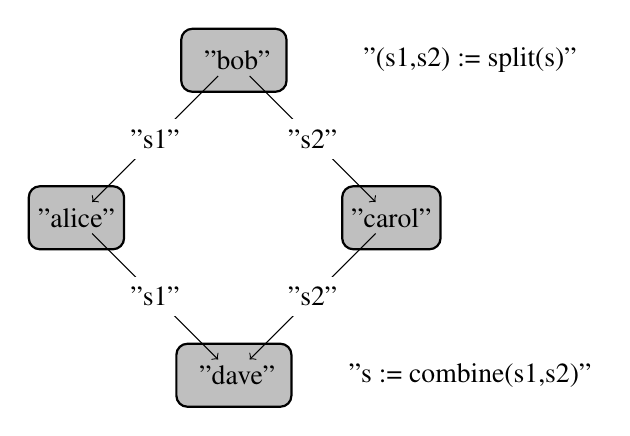
\begin{tikzpicture}
[
mysquare/.style={rectangle, draw=black, fill=gray!50, thick, minimum size=8mm, rounded corners},
tbox/.style={rectangle, draw=white, fill=white, thick, minimum height=0.2cm},
]
\node at (0,0) [mysquare]      (ball3)     {~~"bob"~~};
\node at (3,0) [tbox]      (ball3)     {"(s1,s2) := split(s)"};
\node at (-2,-2) [mysquare]      (ball3)     {"alice"};
\node at (2,-2) [mysquare]      (ball3)     {"carol"};
\node at (0,-4) [mysquare]      (ball3)     {~~"dave"~~};
\node at (3,-4) [tbox]      (ball3)     {"s := combine(s1,s2)"};

\draw[->] (-0.2,-0.2) -- (-1.8,-1.8);
\node at (-1,-1) [tbox]      (ball3)     {"s1"};
\draw[->] (0.2,-0.2) -- (1.8,-1.8);
\node at (1,-1) [tbox]      (ball3)     {"s2"};
\draw[->] (-1.8,-2.2) -- (-0.2,-3.8);
\node at (-1,-3) [tbox]      (ball3)     {"s1"};
\draw[->] (1.8,-2.2) -- (0.2,-3.8);
\node at (1,-3) [tbox]      (ball3)     {"s2"};
%\draw [->,red, very thick] (b4.east) to [out=10,in=330] (b1.east) ;
\end{tikzpicture}
\caption{Not working alice}
%\caption{Overview of $(2,2)$ secret sharing: "bob" shares his secret shares with "alice" and "carol". Later, "alice" and "carol" forward their respective shares to "dave". Finally, "dave" reproduces the initial secret "s" with the shares he received from "alice" and "carol".}
\label{fig:secshrfig}
\end{figure*}


\begin{figure*}
\centering 
\begin{lstlisting} 
splitCombinePassword():
  (s1,s2) := split(s) $@$ bob;$\label{ss:split}$
  send s1 to alice; $\label{ss:send1}$
  send s2 to carol;$\label{ss:send2}$
  con := func();$\label{ss:func}$ $\textcolor{blue}{\textup{// func() returns a bool}}$
  if(con)$\label{ss:ifs}$
    fetch s1 from alice;$\label{ss:get1}$
    fetch s2 from carol;$\label{ss:get2}$
    s' := combine(s1,s2) $@$ dave; $\label{ss:combine}$
  else return;
\end{lstlisting}
\caption{Creating two secret shares from a secret and then reconstructing the secret from the two secret shares using functions of a $(2,2)$ secret sharing protocol.}
\label{fig:motivatesecshr}
\end{figure*}


\subsection{$(2,2)$ secret sharing in \FLAQRp} \label{sec:secshrStart}

Our abstractions for secret sharing in \FLAQRp make use of the
$\retetav{\ell}{}$ term to represent sealed secret shares. 
However, aspects
of secret sharing schemes differ from the use of $\retetav{\ell}{}$ in prior
FLAC-based languages~\cite{jflac,dflate,nmifc}.  Here, in addition to the sealed values
generated by the $\returnp{\ell}$ term, sealed values may also
be created when splitting a secret into shares. In the previous approaches,
a value sealed by $\returnp{\ell}{}$
serves as a reasonable model for signed and encrypted values.  Specifically, the confidentiality component $\ell^{\confid}$ behaves like a public-key encrypted value: anyone can encrypt values at $\ell^{\confid}$, but only authorized parties (which
possess the associated private key) can distinguish the values protected at $\ell^{\confid}$.
Since $\returnp{\ell}{}$ can only be applied in contexts where $\pc \actsfor \ell^{\integ}$
(see \ruleref{UnitM}),
the integrity component behaves like a digitally signed value: only authorized
principals can cause a value to be signed with $\ell^{\integ}$ integrity, but anyone
can use high-integrity values.\footnote{There doesn't appear to be a natural cryptographic
  analog for the availability component.} Obviously then, enforcing these policies
cryptographically would require public-key infrastructure.

Secret sharing behaves differently from the above interpretations: rather
than authorization being based on possession of a long-lived private key (a reasonable
proxy for identity), secret sharing implicitly authorizes \emph{any party} possessing
$t$ shares. Therefore using identity-based principals such as \texttt{alice} or \texttt{bob}
is inappropriate since, even if a shared secret is intended for \texttt{alice},
anyone with $t$ shares will be able to distinguish the secret. Even \texttt{alice}
must have $t$ shares to access the secret. An abstraction for secret sharing should
capture this behavior, but doing so in \FLAQRp requires new concepts.

We extend the set of principals \P\ with new primitive principals $L$
and $R$ representing the left and right shares of our $(2,2)$ secret
sharing scheme. The set of all principals $\P$ for \FLAQRp is thus the
closure of the set $\N \cup \{\top, \bot, L, R\}$ over the same operations as
\FLAQR. In the following we are only interested in the confidentiality
projections $L^{\confid}$ and $R^{\confid}$, since secret sharing only
concerns enforcing the confidentiality of the secret.

Another aspect of secret sharing that departs from prior uses of FLAC
principals is that each time shares are created, they are protected by
a different secret.  Consequently, shares created from different
invocations cannot be mixed, even when the underlying value is the same.
For this reason, we define \emph{key principals}, a new type of principal
generated dynamically at runtime. For our purposes, each $k \in \keys$,
where $\keys$ is the set of all key principals, is equipped with a left
and right principal, $k.L^{\confid}$ and $k.R^{\confid}$. Importantly, since key principals
are generated dynamically, they are not directly representable statically.
The principals $L^{\confid}$ and $R^{\confid}$ are the static representation for the
left and right principals of any key principal, but the shares of different
key principals cannot be distinguished at the type level.


\subsection{Semantics and types for secret sharing}

\begin{figure*}
\begin{flushleft}
\begin{mathpar}

\erule{E-Split}{k \text{ is fresh}}
{\splits{\ell}{v}}{\pair{\returnv{k.L^{\confid} \wedge \ell}{v}}{\returnv{k.R^{\confid} \wedge \ell}{v}}} 

\erule{E-Combine}{}
{\comb{x}{\pair{\returnv{k.L^{\confid}\wedge \ell}{v}}{\returnv{k.R^{\confid}\wedge \ell}{v}}}{pc}{e}}{\subst{e}{x}{v}}
%{\comb{x}{\pair{\returnv{k.L\wedge \ell}{v}}{\returnv{k.R \wedge \ell}{v}}}{\pc}{}}{}
%{\returnv{\ell}{x}}}{y}
%{\returnv{\ell}{v}}

\end{mathpar}
\end{flushleft}
\caption{\FLAQRp semantics for secret sharing (splitting secrets and combining shares).}
\label{fig:secShSem}
\end{figure*}

\begin{figure*}
\begin{mathpar}

\Rule{Split}
{
\TValGpcw{e}{\tau} \\
\rafjudge{\Pi}{c}{pc} \\\\
\drflowjudge{\Pi}{pc}{\ell \join \view{{pc}^{\integ}}}
}
{\TValGpcw{\splits{\ell}{e}}{\prodtype{\says{L^{\confid} \wedge \ell}{\tau}}{\says{R^{\confid} \wedge \ell}{\tau}}}}

\Rule{Combine}
{      
	\TValP{\GG;pc;c}{e}{\prodtype{\says{L^{\confid}\wedge \ell}{\tau}}{\says{R^{\confid}\wedge \ell}{\tau}}} \\\\
	\rafjudge{\Pi}{c}{pc} \\ \TVal{\Pi;\Gamma,x\ty \tau;\ell \join pc;c}{e'}{\says{\ell'}{\tau}} \\\\
	\drflowjudge{\Pi}{\ell \join pc}{\says{\ell'}{\tau}}
}
{
	\TValGpcw{\comb{x}{e}{pc}{e'}}{\says{\ell'}{\tau}}
}


\Rule{SealedK}
{\TValGpcw{v}{\tau}\\\\
\rafjudge{\Pi}{c}{pc} \\ K \in \{L^{\confid},R^{\confid}\}}
{\TValGpcw{\returnv{k.K\wedge\ell}{v}}{\says{K \wedge \ell}{\tau}}}

\end{mathpar}
\caption{\FLAQR$^{+}$ typing rules for secret sharing.}
\label{fig:secShTy}
\end{figure*}




Figure~\ref{fig:secShSem} presents the  semantic rules added to \FLAQRp. Expression $\splits{\ell}{v}$ 
produces two secret shares, sealed with principals $k.L^{\confid} \wedge \ell$ and $k.R^{\confid} \wedge \ell$
from the secret value ${v}$ (rule \ruleref{E-Split}) using
a fresh key principal $k$.
The $\ell$ annotation specifies an additional policy to seal the secret with an addition to
the key principal. Primarily $\ell$ is used for integrity and availability components
since $k.L^{\confid}$ and $k.R^{\confid}$ are confidentiality projections.

Two shares are combined with expression
$$\comb{x}{\pair{\returnv{k.L^{\confid}\wedge \ell}{v}}{\returnv{k.R^{\confid}\wedge \ell}{v}}}{pc}{e}$$
Rule \ruleref{E-Combine} evaluates these terms to $\subst{e}{x}{v}$
revealing the secret $v$ and substituting it for $x$ in the body $e$.
Notice that the key principal is the same on both sides of the
pair. As discussed below in Section~\ref{sec:secshrfail}, mismatched
key principals result in failure. The additional $\pc$ annotation on
combine terms is used by the extended blame semantics, discussed in
Section~\ref{sec:secshrblame}.


For simplicity, our extension only supports \emph{(2,2)-threshold}
secret sharing, but we believe extending this framework to support
\emph{(t,n)-threshold} secret sharing for $2 < n$ and $t < n$ would be
straightforward. 
For example, given some $t$ and $n$, we could
redefine \ruleref{E-Split} to generate a tuple containing $n$ shares
sealed by principals
$k.S_1^{c},k.S_2^{c},...,k.S_n^{c}$. \ruleref{E-Combine} would be
replaced by $n \choose t$ rules: one for each valid $t$-sized
subset of shares.

Figure~\ref{fig:secShTy} presents the \FLAQRp\ 
typing rules for "split" and "combine". The last premise in the \ruleref{Split} rule
involves the \emph{view} of the $\pc$'s integrity, $\view{\pc^{\integ}}$.
The view of a principal was introduced by Ceccetti et al.~\cite{nmifc}
to specify an upper bound on the confidentiality that may be
\emph{robustly declassified}~\cite{zm01b} based on the integrity of
the context performing the declassification and the data itself.
These restrictions ensure an attacker cannot influence what (or whether)
information is declassified. Below, we extend the definition of \emph{view}
with the principals' availability projection counterpart as well.

\begin{definition}[\emph{view} of a principal]
Let $\ell = p^{\confid} \wedge q^{\integ} \wedge r^{\avail}$ be a \textup{FLAM~\cite{flam}} label
(principal) expressed in normal form. The view of $\ell$, written as ${\view{\ell}}$,
is defined as ${\view{p^{\confid} \wedge q^{\integ} \wedge r^{\avail}} \triangleq q^{\confid}}$.
\end{definition}


The premise $\drflowjudge{\Pi}{pc}{\ell \join \view{{pc}^{\integ}}}$
in \ruleref{Split} serves two purposes. First, it ensures the
confidentiality of control flow and the unsealed values in the
context, represented by $\pc$, are no more restrictive than the upper
bound on declassification $\view{\pc^{\integ}}$ (or the confidentiality
of $\ell$ if no declassification takes place).  Second, it ensures the
label $\ell$ protects the availability and integrity of the context; only
confidentiality may be downgraded by "split" terms.

When shares are combined to reveal the secret, the rule
\ruleref{Combine} ensures the combined pair contains a left and right
share (although not which key principal they are associated with), and
that the body of the "combine" term protects the result with a
principal at least as restrictive as the upper bound of $\ell$ and the
context $\pc$ the "combine" occurs in.

In some sense, $\splits{\ell}{}$ and "combine" function as an alternative
to $\returnp{\ell}{}$ and "bind". The difference is that "split" seals
values using a key principal in addition to a label $\ell$, and permits
secrets more restrictive than $\ell$ to be sealed.  Combine is similar to
a "bind" that declassifies its bound value, dropping the key
principals $k.L$ and $k.R$ from the protection requirements on the
body of the "combine".  Note that it is not possible for a type-safe
program to "bind" a secret share. Since a premise of bind would
require the body accessing the unsealed share on host $c$ to typecheck
at $\pc \join (L^{\confid} \wedge \ell)$, this would violate the invariant that $c$ must
act for the $\pc$ of the programs it executes.\footnote{Recall this
  invariant is enforced by the \rafjudge{\Pi}{c}{pc} premise included
  in all typing rules.}


We need one more typing rule, \ruleref{SealedK}, to preserve the types 
of the values sealed with labels $k.L^{\confid}$ 
and $k.R^{\confid}$, for any freshly generated key $k\in \keys$. 
The existing \ruleref{Sealed} rule 
is not enough as it does not handle the values protected with these 
new \emph{key} principals. A consequence 
of this rule is that well-typed \FLAQRp\ programs 
can produce mismatching shares with two different keys 
(say $k_1$ and $k_2$) during run-time. 
We handle mismatching shares with our extended blame semantics, discussed in Section~\ref{sec:secshrblame}.




\subsection{Extending the blame semantics}
\label{sec:secshrfail}
\label{sec:secshrblame}

As with other \FLAQR terms, "fail" values propagate through "split"
and "combine". Figure \ref{fig:secShFail} presents fail propagation
rules for "split" and "combine" statements. These rules are
straightforward propagation rules except for \ruleref{E-CombineFail},
which evaluates to "fail" if the key principals sealing the shares are
mismatched. 

\begin{figure*}
\begin{mathpar}

\erule{E-SplitFail}{k \textup{ is fresh}}
{\splits{\ell}{\faila{\tau}}}{\faila{\prodtype{\says{L^{\confid} \wedge \ell}{\tau}}{\says{R^{\confid} \wedge \ell}{\tau}}}}

\erule{E-CombineFail}{k_1 \neq k_2}
{\comb{x}{\pair{\returnv{k_1.L^{\confid}\wedge \ell}{v}}{\returnv{k_2.R^{\confid}\wedge \ell}{v}}}{pc}{e}}{\subst{e}{x}{\faila{\tau}}}

\erule{E-CombineFailL}{}
{\comb{x}{\pair{\faila{\says{L^{\confid} \wedge \ell}{\tau}}}{f}}{pc}{e}}{\subst{e}{x}{\faila{\tau}}}

\erule{E-CombineFailR}{}
{\comb{x}{\pair{v}{\faila{\says{R^{\confid} \wedge \ell}{\tau}}}}{pc}{e}}{\subst{e}{x}{\faila{\tau}}}

\end{mathpar}
\caption{fail propagation rules in \FLAQRp}
\label{fig:secShFail}
\end{figure*}


\begin{figure*}
  {\footnotesize
\begin{mathpar}
\derule{C-CombineFail}{k_1 \neq k_2 \quad \blame':= \normal{pc , \blame}}
{\concon{\comb{x}{\pair{\returnv{k_1.L^{\confid}\wedge \ell}{v_1}}{\returnv{k_2.R^{\confid} \wedge \ell}{v_2}}}{pc}{\returnv{\ell}{x}}}{c}{s}{\blame}}
{\concon{\faila{\says{\ell}{\tau}}}{c}{s}{\blame'}}
\end{mathpar}
}
\caption{\ruleref{E-CombineFail} with Blame Semantics.}
\label{fig:ccombinefail}
\end{figure*}


The introduction of \ruleref{E-CombineFail} rule creates an additional
source of failure besides "compare" terms with mismatched values.
Rule \ruleref{C-CombineFail} extends \FLAQR's blame semantics to 
account for this. Unlike the case for "compare", we cannot blame the
failure on the principal that sealed the mismatched values given to
"combine".  The failure in this case is due to pairing together shares
generated by different "split" evaluations.  Rather than blaming the
creators of the sealed value, we instead want to blame the principals
that influenced this pairing. This influence is represented by the label
of the $\pc$.  Hence, when $k_1$ and $k_2$ do not match, \ruleref{C-CombineFail} 
adds $\pc$ to the blame set. The function $\L$ used in \ruleref{C-CompareFail}
is unnecessary here because it is unnecessary to examine any subterms of the
combined pair—only the outer key principals contribute to a "combine" failure.

The "NORM" function\footnote{This normalization function was not present in the
  original FLAQR publication~\cite{flaqr}, which is an error. Normalization of
  the statements added to the blame set is required to ensure compound principals
  are correctly handled.} in the premise of \ruleref{C-CombineFail} 
is used to add the new (potentially malicious) 
principal $pc$ in the exisiting blame set $\blame$
in normalized form. 
For example, if $pc = (a \wedge b) \vee c$ and if 
$\blame := (\inF{\ell_1}{\FN}) \OR (\inF{\ell_2}{\FN})$, 
then calling $"NORM"(pc,\blame)$ will return a 
blame set 
\begin{align*}
\blame' := & (\inF{a}{\FN}~"AND"~\inF{b}{\FN}~"AND"~\inF{\ell_1}{\FN})~\OR (\inF{a}{\FN}~"AND"~\inF{b}{\FN}\AND
\inF{\ell_2}{\FN})\\
& \OR(\inF{c}{\FN}~"AND"~\inF{\ell_1}{\FN})\OR(\inF{c}{\FN}~"AND"~\inF{\ell_1}{\FN})
\end{align*}
In case of \ruleref{C-CompareFail} (Figure \ref{fig:ccomparefail}), the "NORM" function was called from within 
the $\last$ function (see Figure \ref{fig:Blameconst}). 
Figure \ref{fig:helperBlameconst} contains the complete definition of
the "NORM" function.

 

\subsection{Security properties}

By design, "split" and "combine" are interfering with respect to confidentiality:
they can cause secret values to be declassified.  However, we would like to
ensure that integrity and availability noninterference are unaffected.


In order to prove integrity and availability noninterference for
\FLAQRp\ programs we extend the bracketed semantics
(Figure~\ref{fig:secShrbracket}) and observation function
(Figure~\ref{fig:secShrobserve}) with rules for "split" and "combine",
and add the corresponding cases for "split" and "combine" terms to the
proofs for the lemmas and theorems of \FLAQRp{}. The noninterference
theorem statements for \FLAQRp{} are identical to
Theorems~\ref{th:ciNI} and~\ref{th:availNI}, though
Theorem~\ref{th:ciNI} only holds for $\pi="i"$ in \FLAQRp{}. Since the
new static principals $L$ and $R$ are only used in confidentiality
projections, rules such as \ruleref{Q-Guard} and the \emph{fails} are
unaffected by the new terms for secret sharing, the proofs of these
theorems is largely unchanged from those for \FLAQR{}.  However,
ensuring the new terms did not break an essential lemma such as
subject reduction (Lemma~\ref{subjRedhost}) required careful design of
the new rules for evaluation, failure propagation, bracketed semantics, and
typing.


Although we protect the robustness (in theory) of what values may be
declassified via "split" and "combine", secret sharing is inherently
non-robust since the party possessing the shares decides whether to
reveal the secret.  To formalize the protections that "split" and 
"combine" do offer, a weaker form of robust
declassification would be required that permits secure uses of
"split" and prohibits insecure ones (such as those violating the premise
$\drflowjudge{\Pi}{pc}{\ell \join \view{{pc}^{\integ}}}$). Such a definition
is not immediately clear\footnote{One reason such a definition is challenging
  in FLAC-based languages is that the $\pc$ label not only protects control flow,
  but also any values that have been unsealed using "bind" (which raises the $\pc$
  label for its body).} to us, and
we leave further investigation to future work.  Since "split" and
"combine" permit non-robust declassification, they could
potentially permit malleability attacks~\cite{nmifc}. 
Since secret shares cannot be unsealed via "bind", the possibility
for such attacks is limited, but we leave formalization of the strength of these limitations
to future work. 

{For "compare" statements, failures are generated because of two mismatching values.
In contrast, the contents of the secret shares are irrelevant in "combine" statements.
Instead, "combine" failures happen due to mismatching keys of the secret shares.  
Hence, we should only blame the control flow of the program for putting 
the two mismatching secret shares together.
Since the program counter tracks the control flow of the program, 
we blame the program counter annotation $\pc$ in the \ruleref{C-CombineFail}
rule by adding it to the blame set when a "fail" term is returned while combining two shares.
Our Theorem \ref{th:failresult0} (Sound blame) still holds, even though "combine" statement
adds a new source of failure.
The new cases hold because the premise $\drflowjudge{\Pi}{\pc}{\says{\ell'}{\tau}}$ in \ruleref{Combine}
allows us to show $\recrafjudge{\Pi}{pc}{\says{\ell'}{\tau}}$ (using \ruleref{P-Lbl}
and \ruleref{A-Avail}). Since, Theorem \ref{th:failresult0} holds, 
Theorem \ref{th:majorityLive} (Majority liveness) holds as well, as it 
depends on Theorem \ref{th:failresult0}.}

\begin{figure*}
\begin{mathpar}
\berule*{B-Split}
{}
{\splits{\ell}{\bracket{v_1}{v_2}}}
{\pair{\returnv{k.L^{\confid} \wedge \ell}{\bracket{v_1}{v_2}}}{\returnv{k.R^{\confid} \wedge \ell}{\bracket{v_1}{v_2}}}}
{}

\berule*{B-Combine}
{}
{\comb{x}{\bracket{v_1}{v_2}}{pc}{e}}{\bracket{\comb{x}{v_1}{pc}{e}}{\comb{x}{v_2}{pc}{e}}}
{}
\end{mathpar}
\caption{Bracketed semantics for \FLAQRp\ terms.}
\label{fig:secShrbracket}
\end{figure*}

\begin{figure*}
\begin{align*}
\observefc{\splits{l}{e}}{\Pi}{\ell}  &=  \splits{l}{\observefc{e}{\Pi}{\ell}} \\ 
\observefc{\comb{x}{\pair{e_1}{e_2}}{pc}{e}}{\Pi}{\ell}  &=  \\
\noalign{$\comb{x}{\pair{\observefc{e_1}{\Pi}{\ell}}{\observefc{e_2}{\Pi}{\ell}}}{pc}{\observefc{e}{\Pi}{\ell}}$}
\end{align*}
\vspace{-1cm}
\caption{Observation function for intermediate \FLAQRp\ terms (extended from FLAC \cite{jflac}).}
\label{fig:secShrobserve}
\end{figure*}

\subsection{Password splitting example with \FLAQRp.}
Figure \ref{fig:secshrexample} presents the \FLAQRp implementation of the 
example discussed in Section \ref{sec:motivsecshr}.
The program executes at host $c'$ with program counter $pc$, such that $\rafjudge{\Pi}{c'}{pc}$.
The host $a$ has program counter $a$, host $b$ has program counter $b$ and
host $c$ has program counter $c$.
The program consists of a function body (lines \ref{exss:lam}-\ref{exss:comb}) 
and an argument to it (line \ref{exss:run}). 
The function body is of type $\func{\tau_b}{pc}{\says{\ell'}{"int"}}$,
where $\tau_b$ = ${\says{b^{{\integ}{\avail}}}
{\prodtype{\says{L^{\confid} \wedge b}{"int"}}{\says{R^{\confid} \wedge b}{"int"}}}}$,
and takes the value of running a "split" statement 
 at host $b$ (i.e. $\runa{\tau_b}{(\splits{b}{v})}{b}$), 
which splits $b$'s secret $v$.
The argument type is $\tau_b$. 

This means the pair of the secret shares created at and returned by $b$ 
is tainted with $b$'s integrity and availability.
In order to typecheck the "run" statement $pc$ needs to flow to $b$, i.e. 
the condition $\drflowjudge{\Pi}{pc}{b}$ needs to hold. 
The condition $\rafjudge{\Pi}{c}{\UB{\prodtype{\says{L^{\confid} \wedge b}{"int"}}{\says{R^{\confid} \wedge b}{"int"}}}}$ 
satisfies trivially, as $\UB{{\prodtype{\says{L^{\confid} \wedge b}{"int"}}{\says{R^{\confid} \wedge b}{"int"}}}}=\bot$.
The function body can be executed at $c'$ as 
$\UB{\func{\tau_b}{pc}{\says{\ell'}{"int"}}}=pc$ and we mentioned earlier that 
the condition $\rafjudge{\Pi}{c'}{pc}$ is true. 
The "run" statements on line \ref{exss:bind2} and \ref{exss:bind3} indicates that the
{left share} is tainted by $a$'s and the {right share} is tainted by $c$'s  
integrity and availability. Which means $a$ and $c$ have seen and approved on the 
secret shares created by $b$. To make the "run" statements on lines \ref{exss:bind2} and \ref{exss:bind3}
well-typed, the conditions  $\drflowjudge{\Pi}{pc}{a}$  $\drflowjudge{\Pi}{pc}{c}$ should satisfy.
We choose label $\ell$ such that $\drflowjudge{\Pi}{pc \join a^{{\integ}{\avail}} 
\join b^{{\integ}{\avail}} \join c^{{\integ}{\avail}}}{\ell}$.
The "bind" statements (lines \ref{exss:bind1}-\ref{exss:bind3}) typecheck because the conditions 
$\drflowjudge{\Pi}{pc \join b^{{\integ}{\avail}}}{\ell}$,
$\drflowjudge{\Pi}{pc \join b^{{\integ}{\avail}} \join a^{{\integ}{\avail}}}{\ell}$
and $\drflowjudge{\Pi}{pc \join b^{{\integ}{\avail}} \join a^{{\integ}{\avail}} \join c^{{\integ}{\avail}}}{\ell}$
hold due to our choice of $\ell$. 

\begin{figure}
\begin{lstlisting}
$\lamc{arg}{\says{b^{{\integ}{\avail}}}{\prodtype{\says{L^{\confid} \wedge b^{{\integ}{\avail}}}{"int"}}{\says{R^{\confid} \wedge b^{{\integ}{\avail}}}{"int"}}}}{pc}{}{}\label{exss:lam}$
$~~{(\bind{s}{arg}{}}\label{exss:bind1}$ 
$~~~~{(\bind{s_1}{(\runa{\tau_{a}}{(\proj{1}{s})}{a})}{}}\label{exss:bind2}$
$~~~~~~(\bind{s_2}{(\runa{\tau_{c}}{(\proj{2}{s})}{c})}{}\label{exss:bind3}$
$~~~~~~~~(\comb{sec}{\pair{s_1}{s_2}}{pc}{\returnv{\ell}{sec}}))))\label{exss:comb}$
$(\runa{\tau_{b}}{(\splits{b^{{\integ}{\avail}}}{v})}{b})\label{exss:run}$
\end{lstlisting}
{\small
\vspace{-1.5em}
\begin{flalign*}
\text{where} \\
  &\tau_{a} = \says{a^{{\integ}{\avail}}}{(\says{L^{\confid} \wedge b}{"int"})}& \\
  &\tau_b   = \says{b^{{\integ}{\avail}}}{\prodtype{\says{L^{\confid} \wedge b}{"int"}}{\says{R^{\confid} \wedge b}{"int"}}}& \\
  &\tau_{c} = \says{c^{{\integ}{\avail}}}{(\says{R^{\confid} \wedge b}{"int"})}&
\end{flalign*}
}
\caption{A simple example of secret sharing in \FLAQRp.}
\label{fig:secshrexample}
\end{figure}


\input{chapters/flaqr/FlameChor2}
\chapter{Locality aware dynamic searchable encryption meets forward and backward privacy}\label{ch:iodse}
We focus on the problem of I/O-efficient Dynamic Searchable Encryption (DSE), i.e., schemes that perform well when executed with the dataset on-disk. Towards this direction, for HDDs, schemes have been proposed with good \emph{locality} (i.e., low number of performed non-continuous memory reads) and \emph{read efficiency} (the number of additional memory locations read per result item). \neww{Similarly,} for SSDs, schemes with good \emph{page efficiency} (reading as few pages as possible) have been proposed. However, the vast majority of these works are limited to the \emph{static} case (i.e. no dataset modifications) and the {only} dynamic scheme fails to achieve forward and backward privacy, the de-facto leakage standard in the literature. In fact, prior related works (Bost [CCS'16] and Minaud and Reichle [CRYPTO'22]) claim that I/O-efficiency and forward-privacy are two \emph{irreconcilable} notions.
% while they propose new I/O efficient Dynamic Searchable Encryption but without forward/backward privacy. 
Contrary to that, in this work, we ``reconcile'' {for the first time} forward and backward privacy with I/O-efficiency for DSE both for HDDs and SSDs. We propose two families of DSE constructions which also improve the state-of-the-art (non I/O-efficient) both asymptotically and experimentally. Indeed, some of our schemes improve the in-memory performance of prior works. \neww{ At a technical level, we revisit and enhance the \emph{lazy de-amortization} DSE construction by Demertzis et al. [NDSS'20], transforming it into an I/O-preserving one. Importantly, we introduce an oblivious-merge protocol that merges two equal-sized databases without revealing any information, effectively replacing the costly oblivious data structures with more lightweight computations.}


%At a technical level, we revisit and improve the \emph{lazy de-amortization} DSE \neww{construction} of Demertzis et al. [NDSS'20] into an I/O-preserving one. Importantly, we \new{introduce an oblivious-merge protocol which merges two equal-sized databases obliviously, and} replaces the costly oblivious data structures.
%with more lightweight and simpler-to-implement oblivious sorting.

%At a technical level, we revisit and refine the \emph{lazy de-amortization} DSE \neww{construction} of Demertzis et al. [NDSS'20] into an I/O-preserving one. Importantly, we \new{introduce a protocol which merges two equal-sized databases obliviously, and} replaces the costly oblivious data structures with more lightweight and simpler-to-implement oblivious sorting. %\todo{1. explain novelty}
%\tblue{add one line about oblivious merge.}
% DSE schemes for HDDs and SSDs, while at the same time 

% In this area, many recent works achieve the  of forward-and-backward privacy; however, none of these simultaneously achieves good I/O-performance when running from disk storage.
% % (forward privacy nullifies the leakage during updates; backward privacy controls during search the leaked information about deleted records).
\section{Preliminaries} \label{sec:prelim}
\noindent\textbf{Notation.} Let $(x';y')\leftrightarrow P(x;y)$ denote a protocol execution between a 
client and a server, {which may consist of multiple rounds of communication}, and $(x';y')\leftarrow A(x;y)$ 
denote an algorithm execution, with no communication between client and server---$x$ and $x'$ are the 
input and output for the client, and $y$ and $y'$ are the input and output for the server.  
We denote by $\lambda \in \mathds{N}$ a security parameter and by $v(\lambda)$ a negligible function in $\lambda$. \textsf{PPT} stands for \textsf{P}robabilistic \textsf{P}olynomial-\textsf{T}ime. $\D$ is a collection of $n$ documents with identifiers $id_1, \ldots, id_n$. A document contains a set of keywords from a dictionary $\Delta$. 
%$D(w)$ is the set of documents that contain keyword $w$.
 %to the set of identifiers of the documents that contain it. Let the database, denoted as $DB$, consists of keyword-identifier  %pairs of the form $\pair{w}{id}$. There are a total of $N$ entries in $DB$.
Let $DB$ consist of $N$ tuples of the form $(w,id,op)$--file $id$ contains keyword $w$, and $op$ is either $add$ or $del$, which denotes whether the tuple is for an insertion or deletion. $DB(w)$ is the set of identifiers of documents that contain keyword $w$. We use $n_w$ to denote $|DB(w)|$, i.e. the result size of keyword $w$. 
The aforementioned tuples can be expanded to $(w,id,op,rank,n_w)$, where $0 \leq rank < n_w$. $EDB$ denotes the encrypted database/index stored in the server. 
   
 %The acronym PPT stands for probabilistic polynomial-time.
 %Our searchable encryption protocols are executed 
 %between a client and a server in an interactive way. 
%  The notation $(x';y')\leftrightarrow P(x;y)$ denotes a protocol 
%  execution, where $x$ and $x'$ are the input and output for the client, and $y$ and $y'$ 
%  are the input and output for the server.

\smallskip\noindent\textbf{Pseudo Random Functions (PRFs) \cite{katz2020introduction}.} A PRF function  $F : {\{0, 1\}}^{\lambda} \times {\{0, 1\}}^{*} \rightarrow
{\{0, 1\}}^{*}$ is a two input function where the first input is the \textit{key} and the second is the input $x$. $F$ can be distinguished from a truly random function by a \textsf{PPT} adversary only with negligible probability $v(\lambda)$.  

% \medskip\noindent\textbf{Pseudorandom Functions.}
% Let $Gen(1^{\lambda}) \in \{0, 1\}^{\lambda}$ be a
% key generation function, 
% and $F : {\{0, 1\}}^{\lambda} \times {\{0, 1\}}^{\ell} \rightarrow
% {\{0, 1\}}^{\ell'}$ be a pseudorandom function (PRF) family. 
% $F$ is a secure PRF family if for all PPT adversaries Adv,
% $|Pr[K \leftarrow Gen(1^{\lambda}); 
% Adv^{F(K,\cdotp)}(1^{\lambda}) = 1]-Pr[Adv^{R(\cdotp)}(1^{\lambda}) = 1]| \leq v(\lambda)$, 
% where $R : {\{0, 1\}}^{\ell} \rightarrow {\{0, 1\}}^{\ell'}$ is a truly random function.


% \begin{figure}
% \begin{tabular}{|c|c|}
% \hline
% symbol & Definition \\
% \hline
% \hline
% $\lambda$ & security parameter \\
% \hline
% $v(\lambda)$ & negligible function in $\lambda$ \\
% \hline
% $w$ & keyword \\
% \hline
% $\Delta$ & dictionary of keywords \\
% \hline
% $n$ & total number of documents \\
% \hline
% $\D = \{d_1, \ldots d_n\}$ & set of documents \\
% \hline
% $\I = \{id_1, \ldots id_n\}$ & set of unique identifiers  \\
% & per document \\
% \hline

% $D:\Delta \rightarrow P(\I)$ & 
%                 $D(w)$ returns the document \\
%                 &  identifiers that contain $w$ \\
%                 \hline
% $\pair{w}{id}$ & keyword-identifier pair \\
% \hline
% $DB$& the database : collection of   \\
% & keyword-identifier pairs, i.e. \\
% & if $id \in D(w)$ then $\pair{w}{id} \in DB$ \\
% \hline
% N & total number of keyword-identifier \\
% & pairs i.e. $N = |DB| = \Sigma_{w\in\Delta}|D(w)|$ \\
% \hline
% $EDB$ & Encrypted $DB$ \\
% \hline
% \end{tabular}
% \end{figure}

\smallskip\noindent{\textbf{Dynamic Searchable Encryption (DSE).}} 
A DSE scheme  $\Sigma$ consists of a $\texttt{Setup}$ algorithm, and (possibly interactive) protocols $\texttt{Search}$ and $\texttt{Update}$--$\Sigma=(\texttt{Setup},\texttt{Search},\texttt{Update})$.
\begin{itemize}
    \item $(K,\sigma ;EDB) \leftarrow \texttt{Setup}(\lambda,N)$ takes as input the security parameter 
    $\lambda$ and $N$. Returns $EDB$ to the server, and the secret key $K$ and local state $\sigma$ to the client.
    
    \item $(res,K,\sigma;EDB) \leftrightarrow\texttt{Search}(K, w, \sigma; EDB)$ is a protocol for searching keyword $w$. The output of this protocol is the query result $res$ (i.e., $DB(w)$). The protocol may or may not modify $K$, $\sigma$ and $EDB$. 
    
    \item $(K,\sigma;EDB) \leftrightarrow\texttt{Update}(K, (w,id,op), \sigma ; EDB)$ is a protocol that inserts/removes $\pair{w}{id}$ to/from the DB--$op = add/del$. The protocol may modify $K$, $\sigma$ and $EDB$. {This protocol modifies $EDB$ and may modify $K$ and $\sigma$.}
\end{itemize}
{{The \texttt{Search} and \texttt{Update} algorithm/protocols for the schemes presented in section \ref{sec:de-amortized} also include an additional parameter $\Gamma$, which is an instance of a static SE scheme}\footnote{\new{$\Gamma$ is a static searchable encryption scheme such that $\Gamma = (\texttt{KeyGen},$ $\texttt{Setup},$ $\texttt{Search})$.}.}}

Following~\cite{bost2016ovarphiovarsigma,bost2017forward,ghareh2018new,SDa}, we start from an empty database. Given an input $DB$ of size $N$, the client populates $EDB$ by calling the $\texttt{Update}$ protocol $N$ times. Other works ~\cite{etemad2018efficient,kim2017forward} equivalently modeled updates in document granularity, i.e., inserting or 
deleting an entire document. We focus on retrieving only the document identifiers upon $\texttt{Search}$; the client may retrieve the documents separately if needed. This leads to a straightforward leakage formulation and is more natural for database queries (e.g.,~\cite{compress,Kamara16,Seal}).

% Following~\cite{bost2016ovarphiovarsigma,bost2017forward,ghareh2018new,SDa}, we assume that we start with an empty database by running $\texttt{Setup}$.Given a $DB$ of size $N$, 
% the client first instantiates the empty database by running $Setup$, 
% followed by $N$ calls to $Update$ to ``populate" the $EDB$. Other works ~\cite{etemad2018efficient,kim2017forward}
% have modeled different definitions of update, e.g. inserting or 
% deleting an entire document from the database. We argue that it is 
% functionally equivalent as it can be decomposed into multiple calls of 
% our version of $Update$. We have also omitted the fact 
% that after performing a $Search$, the client might
% make an additional step to retrieve the actual documents.}


\smallskip\noindent{\textbf{DSE--Leakages \& Forward/Backward privacy.}}
The standard security of a DSE scheme is parametrized by a leakage function $\lp = (\lp^{Stp}, \lp^{Srch}, \lp^{Updt})$. $\lp^{Stp}$ corresponds to the leakage during the setup phase--in our case it reveals size of the database $N$; %\tgreen{the rest have no example} 
$\lp^{Srch}$ corresponds to the leakage during search queries; $\lp^{Updt}$ corresponds to the leakage during update queries. %We discuss  $\lp^{Srch}$ and $\lp^{Updt}$ in more detail below. 
{\emph{Search pattern} leakage reveals which searches
are related to the same $w$, and \emph{access pattern} leakage reveals
$DB(w)$ during a search for $w$. \emph{Access pattern} leakage
is unavoidable if the client retrieves the actual files
with an additional round of communication with the server; schemes
that avoid this leakage (e.g. by storing files in oblivious data structures) 
are referred as \emph{result hiding} schemes.}

A secure DSE scheme with leakage $\lp$ should reveal nothing to an adaptive \textsf{PPT}\footnote{\new{An adaptive \textsf{PPT} decides its next step based on its previously observed leakages/search results.}} adversary about the database $DB$ other than the leakage $\lp$. This is formally captured by a standard real/ideal 
% experiment presented in Figure \ref{fig:games} in the Appendix \ref{append:secGames}---for more details see \cite{ShiNDSS14,ghareh2018new,bost2017forward}.
%@@
experiment presented in the extended version---for more details see \cite{ShiNDSS14,ghareh2018new,bost2017forward}.


%with two games RealSSE, IdealSSE following the definitTion of \cite{ShiNDSS14}.
% \medskip\noindent{\textbf{Leakages.}}
% One of the main design goals of an SE scheme is that the leakages associated with it should be as minimal as it can be. But in order to make the scheme useful for real world applications, some leakages are tolerated. 
% During the setup phase, the (maximum) number of entries of $DB$ 
% %and size of the documents 
% is revealed to the server. This leakage is unavoidable and is called the $total~leakage$. During searches and updates few other kinds of leakages occur. \emph{Search pattern} reveals if two queries are for the same keyword. \emph{Access pattern} reveals the documents in the result of a query. \emph{Total updates} reveals total number of times entries pertaining to a keyword $w$ is inserted and deleted (also referred as $n_w$). \emph{Response length} reveals the number of document identifiers in the query result of a keyword $w$, i.e. it reveals $|D(w)|$ (also referred to as $n_w$).
% ORAM based techniques are most commonly used to hide search and access pattern, while padding is used to hide $n_w$ and $n_w$.
% %\paragraph{\textbf{Leakage profile.}}
% Leakage profile of a particular SE scheme is represented as a collection of these above mentioned leakage patterns. 
% %An SE scheme $\Sigma$ is said to be correct if the returned result is correct for every query \cite{cash2014dynamic}. 
% The security of an SE scheme is parametrized by a leakage function $\lp = (\lp^{Stp}, \lp^{Srch}, \lp^{Updt})$ which captures the information revealed to the server or a passive attacker. $\lp^{Stp}$ corresponds to the leakage during setup phase, $\lp^{Srch}$ corresponds to the leakage during search  queries, and $\lp^{Updt}$ corresponds to the leakage during update queries. A secure SE scheme with leakage $\lp$ should reveal nothing about the database $DB$ other than the leakage, $\lp$, defined for it. \change{This is formally captured by a standard real/ideal experiment with two games RealSSE, IdealSSE following the definition of \cite{ShiNDSS14}.}
Forward and backward privacy~\cite{ShiNDSS14,bost2017forward} have become the de-facto security guarantees for modern DSE.

\noindent\underline{\textit{Forward privacy} (\textbf{FP}):} limits the information revealed due to updates. In particular, an $\lp$-adaptively secure DSE is forward private \textit{iff} the update leakage function $\lp^{Updt}$ can be written as: $\mathcal{L}^{Updt}({op},w,{id})=\mathcal{L'}^{Updt}({op},id)$ where $\mathcal{L'}$ is a stateless function, {$op=add/del$, and $id$ is a file identifier}. {Particularly, it should be impossible to tell whether an insertion is for a new keyword or a previously inserted/searched one}.\newline
\noindent\underline{\textit{Backward privacy} (\textbf{BP}):} ensures that during searches the server does not learn the identifiers of deleted documents that contained the searched keyword $w$. Bost et al.~\cite{bost2017forward} proposed various formulations for this property.
% three types of backward privacy (BP-I, BP-II, BP-III) with different leakage patterns, from Type-I which reveals the least information to Type-III which reveals the most. 
Here, we target backward private schemes that reveal the identifiers of (non-deleted) documents currently containing $w$ (known as $TimeDB(w)$ leakage) and the timestamps and type (i.e. insertion and deletion) of all prior updates for $w$ (known as $Updates(w)$ leakage). This corresponds to the \textbf{BP-II} definition from~\cite{bost2017forward} %(see Appendix \ref{append:BP} for more details). 
%@@
(see the extended version for more details).
{$TimeDB(w)$ accounts for the leakage from retrieving the actual files; but we focus only on retrieving the document identifiers during \texttt{Search}, and we never use it in our proofs as none of our constructions explicitly leaks $TimeDB(w)$.

\begin{definition}[\cite{bost2017forward}] \label{def:adpSec}
{A DSE scheme $\Sigma$ is $\lp$-adaptively-secure with forward and backward privacy, 
\textit{iff} $\mathcal{L}^{Updt}({op},w,{id}) = \mathcal{L}^{'}({op})$ 
and $\mathcal{L}^{Srch}(w)$  $=\mathcal{L}^{''}({TimeDB}(w),{Updates}(w))$ 
\textbf{and} \textit{iff} for any adaptive \textup{\textsf{PPT}} adversary $\adv$ 
~issuing polynomially many queries $q$, there exists a stateful \textup{\textsf{PPT}} simulator 
\textup{$\sim$}=$(SimSetup,~SimSearch,~SimUpdate)$ such that 

$|\Pr[{Real}^{\textsf{\emph{DSE}}}_{\adv}(\lambda,q)=1]-\Pr[{Ideal}^{\textsf{\emph{DSE}}}_{\adv,\sim,\mathcal{L}}(\lambda,q)=1]| < v(\lambda)$, where $\mathcal{L}^{'}$ 

and $\mathcal{L}^{''}$ are stateless functions; $op$ is insertion or deletion, and $id$ is a file identifier.}
% (BP-II_ functionand it is forward    scheme that supports single-keyword additions/deletions is forward private \textit{iff} the update leakage function  $\mathcal{L}^{Updt}$ can be written as:
% $\mathcal{L}^{Updt}({op},w,{id})=\mathcal{L'}^{Updt}({op},id)$
% where $\mathcal{L'}$ is a stateless function, {$op=add/del$, and $id$ is a file identifier}.
\end{definition}

% document $d$ containing keyword $w$ is deleted before a search for
% $w$, then the result of this search does not reveal anything about $d$. Backward privacy is categorized into three types. (a) Type-I/BP-I reveals only the identifiers of documents currently containing the searched keyword and timestamp of when the documents were inserted, (b) Type-II/BP-II additionally reveals the timestamps and type (i.e. insertion and deletion) of all prior updates for the searched keyword, (c) Type-III/BP-III also reveals for each deletion which insertion it canceled. 
% The following definitions will help us formally define backward privacy ~\cite{bost2017forward}.


%Dynamic symmetric searchable encryption (DSE) leaks additional information to what described above due to the update queries. 
% A dynamic SE is considered to be secure if it satisfies two additional security notions: forward and backward privacy.
% A scheme is forward private if an update does not reveal if the keyword
% pertaining to this update have been queried before. Achieving forward privacy for dynamic SE schemes is important as otherwise it suffers from adversarial document-injection attacks \cite{Seal}. 


% \begin{definition}[\cite{bost2017forward}]
% An $\mathcal{L}$-adaptively-secure DSE scheme that supports single-keyword additions/deletions is forward private \textit{iff} the update leakage function  $\mathcal{L}^{Updt}$ can be written as:
% $\mathcal{L}^{Updt}({op},w,{id})=\mathcal{L'}^{Updt}({op},id)$
% where $\mathcal{L'}$ is a stateless function, {$op=add/del$, and $id$ is a file identifier}.
% \end{definition}


% Backward privacy ensures that if a
% document $d$ containing keyword $w$ is deleted before a search for
% $w$, then the result of this search does not reveal anything about $d$. Backward privacy is categorized into three types. (a) Type-I/BP-I reveals only the identifiers of documents currently containing the searched keyword and timestamp of when the documents were inserted, (b) Type-II/BP-II additionally reveals the timestamps and type (i.e. insertion and deletion) of all prior updates for the searched keyword, (c) Type-III/BP-III also reveals for each deletion which insertion it canceled. 
% The following definitions will help us formally define backward privacy ~\cite{bost2017forward}.

% \change{Let $Q$ be a list that has one entry for each query executed. The entry for a search is of the form $(u,w)$ where $u$ is the query timestamp and $w$ is the searched keyword. Entry for an update is $(u,op,(w,id))$.
% %where $op=add/del$ and $id$ is the document identifier.
% For a keyword $w$, the function \textbf{TimeDB}($w$) returns 
% the list of all timestamp/identifier pairs of keyword $w$ that have been added to $DB$ and not subsequently deleted. }
% \begin{align*}
% \textbf{TimeDB}(w) = \{(u, {id}) \;| \;(&u, {add}, (w, {id})) \in Q \\ &\text{and }
% \forall u', (u', {del}, (w, {id})) \notin Q\}
% \end{align*}
% \textbf{Updates}($w$) function returns the timestamp of all insertion and deletion operations for $w$ in $Q$. 
% \begin{align*}
% \textbf{Updates}(w) =& \{u | (u, {add}, (w, {id})) \in Q \\
%  & \text{ or }~(u, {del}, (w, {id})) \in Q\}.
% \end{align*}
% Funtion \textbf{DelHist}($w$) returns all 
% (insertion timestamp, deletion timestamp) pairs revealing
% which deletion corresponds to which insertion for keyword $w$. 
% \begin{align*}
% \textbf{DelHist}(w) = \{(u^{add},u^{del})\; | \;&\exists\; {id} : (u^{add}, {add}, (w, {id})) \in Q\\ &\text{and }
% (u^{del}, {del}, (w, {id})) \in Q\}
% \end{align*}
% It is clear that the leakage of these three functions is progressively increasing. 
% We are now ready to formally define backward privacy with different types of leakage.

%The strongest backward privacy definition is the type I which reveals just currently existing documents having keyword $w$, their insertion time, and the total number of updates on each keyword. The formal definition of this statement is:

% \begin{definition}[\cite{bost2017forward}]\label{def-bp1}
% An $\mathcal{L}$-adaptively-secure SE scheme has backward privacy:

% 	\begin{itemize}
% 		\item []\textbf{Type-I} \textbf{(BP-I):} \textit{iff} $\mathcal{L}^{Updt}({op},w,{id}) = \mathcal{L}^{'}({op})$, and\\
% 		$\mathcal{L}^{Srch}(w) = \mathcal{L}^{''}(\textbf{TimeDB}(w),n_w)$.
% 		\item[] \textbf{Type-II}\textbf{ (BP-II):} \textit{iff} $\mathcal{L}^{Updt}({op},w,{id}) = \mathcal{L}^{'}({op},w)$, and
% 		$\mathcal{L}^{Srch}(w) = \mathcal{L}^{''}(\textbf{TimeDB}(w),\textbf{Updates}(w))$.
% 		\item[] \textbf{Type-III (BP-III):}		\textit{iff}\\ $\mathcal{L}^{Updt}({op},w,{id}) = \mathcal{L}^{'}({op},w)$, and\\	$\mathcal{L}^{Srch}(w) = \mathcal{L}^{''}(\textbf{TimeDB}(w),\textbf{DelHist}(w))$.	
% 	\end{itemize}

% where $\mathcal{L}^{'}$ and $\mathcal{L}^{''}$ are stateless {functions}.
% \end{definition}
% \change{
% Note that the above definition assumes schemes leak the documents that
% currently contain $w$ in order to account for the leakage from actually retrieving the files. Namely, \textbf{TimeDB}($w$) function explicitly reveals the indexes of  returned documents.} 
% %While none of our schemes reveals this information directly, we still account for it as
% %part of our leakage.

\smallskip\noindent{\textbf{DSE for HDDs: Locality/Read-Efficiency/Update Locality/Update Cost/Space}.}
To scale SE to big data using external memory (i.e., HDD drives),  SE schemes with ``small'' locality and read efficiency have been proposed before. \emph{Locality} is defined as the number of \emph{non-contiguous} memory accesses made during the search by the server. \emph{Read-efficiency} is the ratio of the total amount of data read/retrieved during the search over the actual query result size (for querying a keyword $w$)---see \cite{cash2014locality} for formal definitions. 
%Cash and Tessaro \cite{cash2014locality} proved that in any secure SE scheme with both optimal locality $\bO(1)$ and optimal read efficiency $\bO(1)$ requires $\omega(N)$ space. The intuition behind this lower bound is that in a scheme with optimal locality, read efficiency and linear space, an attacker/server can observe the locations of some queries, as well as the non-accessed ones and infer statistical information about the entire input dataset, i.e., learn information about queries which we have not requested. 
Cash and Tessaro \cite{cash2014locality} proved that any secure SE scheme with both optimal locality $\bO(1)$ and optimal read efficiency $\bO(1)$ requires $\omega(N)$ space. %The intuition behind this lower bound is that schemes with optimal locality, read efficiency, and linear space allow attackers/servers to infer statistical information about the entire input dataset (even for non-requested queries) using information about some accessed queries and observing the non-accessed memory locations. 
%\todo{6.Give the definition of I/O efficiency metrices }
For locality-aware DSE schemes, in addition to the "search" and "static" efficiency, i.e., (i) locality, (ii) read-efficiency and (iii) space, we focus on two update metrics: (iv) update-locality, i.e., the number of \emph{non-contiguous} memory accesses during an update and (v) update asymptotic cost, i.e., the {asymptotic} cost of one update (i.e., insert/delete one $(w,id,op)$ tuple). 
%See Appendix \ref{append:metrics} for the exact definitions.
%@@
See the extended version for the exact definitions.

%\tgreen{the text here sounds like locality and update cost are novel definition}
%\tpurp{--I dont think so.}

% \begin{itemize}
%     \item \emph{Update Locality:} is defined as the number of \emph{non-contiguous} memory accesses during an update.
%     \item \emph{Update Overhead:} is defined as the cost/overhead of one  update (i.e., insert/delete one $(w,id,op)$ tuple).\footnote{Other works consider batch updates (or operate in document granularity). For that case, we can define  \emph{Update Efficiency} as the ratio of the total amount of data read/retrieved during a batch of updates over the batch size.}
% \end{itemize}


% \emph{Update Locality:} The number of total \emph{non contiguous} memory accesses during an update  \\ 
% \emph{Update Overhead:} The ratio of total amount of data read (retrieved) during an update
%                             to the actual amount of data that corresponds to the update 

% The amount of space required to store EDB is called its $space~overhead$. The ideal goal is to construct an SE scheme with optimal space overhead ($\bO(N)$), optimal locality ($\bO(1)$), and optimal read efficiency ($\bO(1)$). But Cash and Tessaro \cite{ct14} proved that achieving optimality in all these three metrices is impossible. Specifically, they prove a lower bound: ``any scheme must be sub-optimal in either its space overhead, its locality, or its read efficiency". 

% \paragraph{\textbf{Dynamic Locality-aware SSE.}}
% Unlike static SE schemes, for Dynamic Locality-aware schemes no such lower bound 
% has been proven yet. Moreover, as DSE schemes support updates, we formally define 
% two new metrices : \\
% \emph{Update Locality:} The number of total \emph{non contiguous} memory accesses during an update  \\ 
% \emph{Update Overhead:} The ratio of total amount of data read (retrieved) during an update
%                             to the actual amount of data that corresponds to the update 

\smallskip\noindent{\textbf{DSE for SSDs: Page-Efficiency/Space}.}
Bossuat et al. \cite{BFF21} proposed a new I/O-efficiency dimension for SSDs, which is called \emph{page efficiency}---SSD performance mainly depends on page efficiency, aiming at reading as few memory pages as possible. More formally, \emph{page efficiency} is the ratio of the total number of pages that the server accesses (using SE) over the optimal number of accessed pages in a plaintext case. %\todo{6. Give the definition of I/O efficiency metrices } 
For page-efficient DSE schemes, in addition to the "search" and "static" efficiency dimensions, i.e., (i) page-efficiency and (ii) space, we focus on (iii) update efficiency, i.e., the number of pages accessed 
 during one update (i.e., insert/delete one $(w,id,op)$ tuple) and (iv) update asymptotic cost (i.e., {asymptotic cost} of insert/delete of one $(w,id,op)$ tuple).
%See Appendix \ref{append:metrics} for the exact definitions.
%@@
See the extended version for the exact definitions.



%@@ more detailed explanation Page Efficient literature
% \tblue{
% \noindent{\textbf{DSE for SSDs--Page-Efficiency/Space}.}
% Locality and read efficiency are not meaningful metrics when solid state drives (SSD) are used as the underlying 
% storage device. For SSDs, the memory accesses are done in terms of memory pages, and the performance 
% is mainly determined by the number of these pages accessed, regardless of whether they are contiguous 
% pages or not. Bossuat et al. \cite{BFF21} present a new criterion called \emph{page efficiency} 
% to capture performance of an SE scheme whose data is stored on SSDs.
% The \emph{page efficiency} is defined as the number of pages that 
% the server must access to process a client's query, 
% divided by the number of pages of the plaintext answer to
% the query. In the same paper the authors presented a \emph{page efficient} static 
% searchable encryption scheme (\textbf{PE-SE}) called Tethys. 
% Storage efficiency in this model is the number of
% pages needed to store the encrypted database, divided by the number of 
% pages of the plaintext database. Tethys offers $\bO(1)$ page efficiency 
% and $\bO(1)$ storage efficiency, but the client storage is not optimal $ \bO{p \log \lambda}$,
% where $p$ is the page size and $\lambda$ is the security parameter. 
% The authors in \cite{BFF21} claims that page efficiency is 
% an excellent predictor of SSD performance and they supported their claim with experiments as well.
% In~\cite{LocalLayeredSSECrypto22} Minaud and Reichle presented two DSE schemes.
% The first one is a dynamic page efficient SE (\textbf{PE-DSE})
% scheme, called \LayeredSSE, that offers 
% \tpurp{$\bO(\log \log N )$} page efficiency, and $\bO(1)$ storage efficiency and client 
% storage. The second scheme takes a PE-SE scheme as 
% an input parameter and runs it along with an overflowing SE (which they call OSSE) scheme. 
% %The basic idea is that if a keyword list overflows, then the 
% %overflowing items will be stored in 
% %the PE-SE scheme, rest will be stored in the OSSE scheme.
% They use a variant of One-Choice Allocation as their OSSE scheme, 
% that supports new updates but ignores the overflowing items.
% There are $\log N$ instances of the PE-SE scheme. If a keyword-list
% of size $k$ overflows then the overflowing items
% go to $\ceil{\log{k}}^{th}$ instance of PE-SE.
% This scheme offers $\bO(1)$ locality, 
% $\bO(1)$ storage efficiency, and \tpurp{$\bO(\log \log N )$}
% read efficiency, but under the condition that the longest list
% is of size $N^{1-\frac{1}{\log \log N}}$. These schemes do not
% ensure $FP$ and $BP$.
% }
% \tblue{
% For PE-DSE schemes, we classify the \emph{page efficiency} metric into two:
% \emph{Search Page Efficiency} and \emph{Update Page Efficiency}.
% \begin{itemize}
%  %\itemsep-0.3em 
%  \item \emph{Search Page Efficiency:} the number of pages that 
% the server must access to process a search query, 
% divided by the number of pages of the plaintext answer to the search query
%  \item \emph{Update Page Efficiency:}  the number of memory pages accessed 
%  during one update (i.e., insert/delete of one $(w,id,op)$ tuple).%\footnote{Similar to \emph{Update Efficiency}, one can define  \emph{Update Page Efficiency} as the ratio of the total number of pages read/retrieved during a batch of updates over the size of the batch in terms of pages.}
% \end{itemize}
% }

\smallskip\noindent{\textbf{Oblivious sort.}}
An oblivious sorting algorithm sorts an array of $N$ elements without leaking information about the relative ordering of the input elements \cite{aks,zigzag,bitonic,ngai2024distributed}. We use the oblivious bucket sort~\cite{bucketSort}, 
which has $\bO(N \log N$) time complexity, and uses a temporary client 
storage { of two buckets, where one bucket contains} 512 elements. 
%and merge sort as the \emph{non-oblivious} sort that bucket sort requires for the last step. 
We can decompose bucket sort into $N \log N/\gamma$ rounds of $\bO(\gamma)$ work per round (e.g., for $\gamma = O(\log N)$ the oblivious bucket sort can be completed in $N$ rounds). We highlight that fetching $\bO(\gamma)$ elements from disk requires always $\bO(1)$ locality, since accesses are performed on a {bucket granularity}, \new{and on consecutive buckets}---
%see Figure \ref{fig:bucketSort} and \ref{fig:mergeSort} in the Appendix \ref{append:bucketLoc} for more details.
%@@
see the extended version for more details.

%@@ More detailed discussion for o-sort 
%



\smallskip\noindent{\textbf{Oblivious compaction.}}
Given an array of $N$ elements, some of which are tagged with bit 1, and the rest 
with bit 0, an oblivious compaction \cite{compact1,compact2,godrichOblComp} 
generates an output in which all the 
elements tagged with bit 1 appear before all the elements tagged with bit 0, without leaking the information of which elements were tagged with bit 1 or 0.  
Our constructions need the compaction to be
order preserving, i.e. the relative ordering of the elements tagged with bit 1/0 do not change after the compaction. We use the oblivious bucket sort~\cite{bucketSort} mentioned above for performing order preserving compaction.


\smallskip\noindent\textbf{Oblivious Maps}($\textsc{OMAP}$)\cite{wang2014oblivious,dauterman2021snoopy}.
%\label{append:omap}
An oblivious map is a data structure that supports oblivious read/get and write/put functionality for encrypted $(key,value)$ pairs (i.e., oblivious hash map). That is, all same-length operation sequences appear indistinguishable. $\textsc{OMAP}$ has the following algorithms/protocols: (i) $\textsc{OMAP}$.$\texttt{Setup}$ initializes an empty data structure with maximum capacity $N$ blocks, (ii) $\textsc{OMAP}$.$\texttt{put}$ adds/overwrites a $(key,value)$ pair, and (iii) $\textsc{OMAP}$.$\texttt{get}$ returns the $value$ of a given $key$. We have used the AVL tree based implementation by Wang et al.~\cite{wang2014oblivious} on top of PathORAM~\cite{stefanov2013path}. For a map with capacity $N$, each oblivious access requires $\bO(\log^2 N)$ operations/accessed-blocks, $\bO(\log N)$ roundtrips, and $\bO(\log^2 N)$ locality---see~\cite{wang2014oblivious} for more details. 

% Goodrich’s oblivious compaction algorithm \cite{godrichOblComp} runs in time $\bO(N \log N)$ 
% and is order-preserving.
% This algorithm accesses array locations in a fixed order using a $\log N$ deep routing network that
% shifts each element a fixed number of steps in every layer. 
%\tpurp{check the paper to see how to de-amortize it, or we can 
%replace it with bucket oblivious sort, which has the same time complexity}


% \paragraph{\textbf{Oblivious sort.}}
% An oblivious sorting algorithm is a sorting algorithm that always compares the elements in the input dataset in the same order regardless of their values. Bitonic sort (also known as Batcher's sort)~\cite{bitonicsort}, is an oblivious sorting algorithm which sorts $N$ elements in $\bO(N\log^2 N)$ time.
% %and with $\bO(\log^2 N)$ locality. 
% The algorithm assumes $N$ to be in power of 2 (padded if not). It \textbf{\textit{compares-and-swaps}} elements in $\log N$ phases. The $i$th phase has $i$ subphases, with $\frac{N}{2}$ \textit{compare-and-swap}s in each subphase. Hence a total of - $$\frac{N}{2}\cdot{\sum_{i=1}^{\log N}i}=\frac{N}{2}\cdot \frac{\log N (\log N +1))}{2}= \frac{N \log N (\log N +1)}{4}$$ \textit{compare-and-swap}s are required to produce a sorted output. Because, the \textit{compare-and-swap}s happen in a fixed schedule, the algorithm can be decomposed into fixed number of rounds, with fixed number of \textit{compare-and-swap}s in each round. For instance, if we decide to execute $\gamma$ number of \textit{compare-and-swap}s per round (ideally $\gamma$ divides $\frac{N \log N (\log N +1)}{4}$ ) then the algorithm will need $\ceil{\frac{N \log N (\log N +1)}{4\gamma}}$ rounds to complete. In one of our schemes the client downloads the necessary $2\gamma$ elements, to perform the $\gamma$ \textit{compare-and-swap}s, then it encrypts those elements with fresh encryptions and sends them back to the server.


% Asharov et al.~\cite{bucketSort} presents an oblivious bucket
% sort that sorts the elements in three steps: 
% \emph{Oblivious Random Bin Assignment (ORB)}, \emph{Oblivious Random Permutation (ORP)}
% and \emph{Non-oblivious Sorting}. During \emph{ORB} the elements are 
% assigned a random key and are randomly distributed into $B$ buckets with $Z/2$
% elements in each bucket ($B= 2N/Z$). $Z/2$ dummy elements are added in each of the bucket. Then, $\log B +1$ rounds of merge-splits are performed, 
% with $B/2$ merge-splits in each round. The main idea is that, 
% during the $i^{th}$ round of merge-splits, every two buckets 
% at distance $2^i$ are fetched by the client and their elements are
% assigned to correct output buckets based on the $i^{th}$ bit 
% of their random key. The two output buckets are written back to level $i+1$.
% During the \emph{ORP} step, 
% each bin is fetched separately by the client, 
% their dummy elements are removed and the real elements are permuted. The \emph{ORP} can be combined together with the last round of $OBA$ . Once all the bins are permuted, any \emph{non-oblivious} sort can be performed to sort the elements. They have proved that composition of these three steps results into an \emph{Oblivious sort}.
% As a total of $B/2 (\log B +1)$ merge-splits are performed, the runtime 
% of this algorithm is $\bO(N\log N)$, if the \emph{non-oblivious} sort
% also has $\bO(N \log N)$ runtime. In our construction
% we have used merge sort as the \emph{non-oblivious} sort. 
% Since elements of a bucket are 
% always stored in contiguous memory locations,
% locality of fetching a bucket is always $\bO(1)$. 

%\todo{7.Clarify which scheme targets which storage and which metrices}
%\todo{20. Explain 1C/2C/NlogN in depth. Explain what superbin is.} 

%\smallskip
\smallskip\noindent{\textbf{One-Choice Allocation.}}
Asharov et al.~\cite{onechoice} presented 
the One-Choice Allocation scheme 
(we will refer to it as \OneChoice) that offers optimal locality,
optimal space overhead and $\bO(\log N \log \log N)$ read efficiency.
Given a database of size $N$, this scheme allocates an 
array of $m={N}/{\log N \log\log N}$ bins, each of 
size $3\log N \log \log N$\footnote{\new{The bins overflow with negligible probability when the bin size is set to $3\log N \log \log N$ for \OneChoice}.}. For each keyword $w$ it computes a hash value $h(w)$, and stores the $i^{th}$ document identifier
in the bin $(h(w) + i)mod~m$. Bins are filled up with $dummy$ entries, if not full.
% The formal description of 1C is provided 
% in Figure \ref{alg:1C}, and Figure \ref{fig:allSEschemes} shows an example in the Appendix. 
%@@
The formal description of 1C is provided the extended version. 
%in Figure \ref{alg:1C}, and Figure \ref{fig:allSEschemes} shows an example in the Appendix. 


\smallskip\noindent{\textbf{Two-Choice Allocation.}}
Asharov et al. also presented the Two-Choice Allocation 
(\TwoChoice) in \cite{onechoice}.
For a database of size $N$, this scheme offers optimal locality and space overhead and 
$\bO((\log\log N)^A(\log$$\log$$\log N)^2)$ read efficiency 
assuming keyword list sizes $<N^{1-1/(\log\log N)^A}$, 
for a constant $A \geq 1$. This scheme allocates an 
array of $m={N}/{(\log\log N)^A (\log \log \log N)^2}$ bins, each bin with  
size $z{\cdot}(\log\log N)^A$ ($\log$$\log$$\log N)^2$, where $2\leq z \leq 4$ (we use $A=1$).
The keyword lists are padded to be nearest power of 2 and stored in decreasing length order. 
For list for $w$, first
it divides bins into groups of $sb = \frac{m}{n_w}$ \emph{superbins}; \neww{i.e. each \emph{superbin} consists of $n_w$ bins.} Then two superbins are chosen with two hash functions: 
$h_1(w)\% sb$ and $h_2(w)\%sb$. \neww{Finally,} the superbin that has \neww{minimal load} stores the list for $w$. 
%Formal description \neww{and an example} of 2C are in Figures \ref{alg:2C} \neww{and \ref{fig:allSEschemes}} in Appendix. 
%@@
The formal description of 2C is provided the extended version. 

\smallskip\noindent{\textsf{\textbf{NlogN}} \textbf{Scheme.}}
The third scheme presented by Asharov et al. in~\cite{onechoice} 
offers optimal locality and read efficiency at the cost of
$\bO(\log N)$ storage overhead, i.e. a total of $\bO(N\log N)$ storage. We highlight this scheme provides optimal page efficiency. This scheme consists of $(\log N +1)$ hash tables, each of size $N$. The keyword-lists are padded so that their length becomes 
nearest power of 2. The $k^{th}$ hash-table stores lists of size $2^k$.  
%The pseudocode of the \NlogN\ scheme is provided in Figure \ref{alg:NlogN}, and Figure \ref{fig:allSEschemes} shows an example in the Appendix. 
%@@
The pseudocode and more details of the \NlogN\ scheme are provided in the extended version. %Figure \ref{alg:NlogN}, and Figure \ref{fig:allSEschemes} shows an example in the Appendix. 
Demertzis et al. \cite{Demertzis17} proposed a variation of the \NlogN\ scheme in which only $s$ of the above mentioned hash tables are stored; $s$ is evenly distributed (i.e. the server stores the levels $\{0, x, 2x, \ldots (s-1){\cdot}x \}$, 
where $x$ is set to be $\lceil{\frac{\log N+1}{s}}\rceil$). In the worst case, 
a keyword-list is divided into smaller $\bO(N^{\frac{1}{s}})$ chunks. 
This scheme achieves optimal read efficiency, $\bO(N^{\frac{1}{s}})$ locality and 
has a $\bO(s)$ space overhead, and $\bO(\text{min}\{N^{\frac{1}{s}}/p, p\})$ page efficiency ($p$ denotes the memory page size). We refer to this scheme as \sN.






%  levels starting from 
% level 0, instead of storing $\ell = (\log N+1)$ levels
% (where $s$ can be as small as 2). Specifically, a value of $p$ is set to be $\ceil{\frac{\ell}{s}}$, 
% and the server stores the levels $\mathcal{L} = \{0, p, 2p, \ldots (s-1){\cdot}p \}$.
% The keyword-list of a keyword $w$ is divided into smaller chunks 
% of size $2^j$ and stored in the level $j$ if $2^j \leq |DB(w)| < 2^i$ for $i,j\in \mathcal{L}$.
% This idea is first introduced in \cite{Demertzis17}
% by We will refer to this scheme as \textsf{Ns}.
% This scheme achieves optimal read efficiency, $\bO(N^{\frac{1}{s}})$ 
% locality and has a $\bO(s)$ space overhead.}



%\tpurp{Description of \Tethys\ is in the appendix.}




%\paragraph{\textbf{LayeredSSE}.}
\smallskip\smallskip\noindent{\textbf{Encrypted dictionary.}}
\new{In our DSE constructions (in section \ref{sec:dseio}) along with the 
encrypted index we have an encrypted dictionary. The 
encrypted dictionary maintains a keyword to keyword-counter 
mapping, i.e. keyword $w$ maps to $|DB(w)|$. To perform searches 
in \OneChoice, \TwoChoice, \NlogN, and \Ns\ schemes the keyword-counter
is required (to know how many bins to fetch, or which levels to search). 
%Because our DSE constructions in section 
%\ref{sec:dseio} use these above mentioned static SE schemes, we needed to 
%maintain this encrypted dictionary as well. 
We will refer to the encrypted 
dictionary as $EDB.\Dict$ and the encrypted index as $EDB.\Index$. % in the rest of the paper.
For an index with $N$ entries the size of $EDB.\Dict$ is at most $N$,
as there can be at most $N$ distinct keywords.}

%\tblue{We should decribe the $EDB.\Dict$ briefly here, it will 
%help us describe the locality/read-efficiency in section \ref{sec:SDalocality}}

%\paragraph{Result hiding SE.} \tblue{Add a short description of it. }
% In a response-hiding scheme, the adversary can not infer
%whether two different responses have overlapping records, thus
%making reconstruction harder. \tred{I think we should not use the term "result-hiding" (result-pattern hiding) at all}
\section{DSE---I/O efficiency meets Forward/Backward Privacy}\label{sec:dseio}
%This section presents our I/O efficient DSE schemes which are the first that achieve both good I/O performance and forward/backward privacy. In Section \ref{sec:SDalocality}, we use
% the \SDa\ transformation proposed by Demertzis et al.\cite{SDa} which transforms static SE schemes to dynamic ones with forward/backward privacy. 
% Our observation is that if we use I/O efficient static SE schemes in the \SDa\ transformation, then the I/O efficiency will be preserved in the produced dynamic ones while maintaining forward/backward privacy. In Sections \ref{sec:de-amortized}, we focus on the more challenging task of providing de-amortized I/O efficient constructions with forward/backward privacy; we provide a new \emph{oblivious merge} framework which achieves the above goals, and we provide three instantiations of this framework---the dynamic de-amortizated \OneChoice, \TwoChoice, and \NlogN\ schemes. 
\neww{
This section introduces our I/O efficient DSE schemes, which are the first to simultaneously achieve good I/O performance and forward/backward privacy. In Section \ref{sec:SDalocality}, we apply the \SDa\ transformation, as proposed by Demertzis et al.\cite{SDa}, in conjunction with I/O efficient static SE schemes. In Section \ref{sec:de-amortized}, we address the more challenging task of offering de-amortized I/O efficient constructions that ensure forward/backward privacy. Here, we introduce a novel \emph{oblivious merge} framework to meet these objectives and present three implementations of this framework: the dynamic de-amortized \OneChoice, \TwoChoice, and \NlogN\ schemes.}


%Later in section \ref{sec:eval} we show our experimental evaluation for these schemes along with the \sN\ scheme for some specific values of s.
%\tgreen{What about \sN scheme?}





\subsection{Amortized Constructions using \SDa \textup{\cite{SDa}}\label{sec:SDalocality}}

\noindent{\textbf{Overview of \SDa[$\cdot$].}} 
% \todo{2. general overview of the transformation} 
% Recently, Demertzis et al~\cite{SDa} proposed a generic compiler called \SDa~that yields a forward/backward private DSE scheme from any result hiding static SE scheme. 
% The high-level idea of \SDa~is that the result of  $N$ updates is stored as a 
% collection of $\log N $ indexes (0$th$ through $(\log N-1)th$),
% where the $i$th index (denoted as $EDB_i$) is of size $2^{i}$. For each new update
% the client runs the \texttt{Setup} of the underlying static SE
% scheme to create an index of size 1 (i.e. $EDB_0$).
% Whenever two indexes of the same size (say $z$) exist, 
% they are downloaded by the client, and the setup of the
% static scheme is called to ``merge'' them into a
% single new index of size $2z$, amortizing the cost of updates.
% Searches are 
% performed in each index independently.  
% In Figure \ref{fig:SDaex1}, we provide an example of an update in \SDa. 
Demertzis et al.~\cite{SDa} introduced a compiler, \SDa, that converts any result hiding static SE scheme into a forward/backward private DSE scheme. The essence of \SDa\ is to store the results of $N$ updates across $\log N$ indexes (ranging from 0$th$ to $(\log N-1)th$). The $i$th index ($EDB_i$) has a size of $2^{i}$. With each update, the client initializes the static SE scheme (using SE's \texttt{Setup}) to produce and upload an encrypted index with size 1 ($EDB_0$). When two same-sized indexes emerge (in server), the client downloads, decrypts and combines them into a doubled size index, amortizing the cost of updates. Searches are performed in each index independently. Figure \ref{fig:SDaex1} shows an update example using \SDa. 
%The optimized pseudocode for \SDa, as depicted in Figure \ref{fig:SDaex1}, can be found in Figure \ref{fig:Scheme1} in the Appendix.
%@@
The optimized pseudocode for \SDa, as depicted in Figure \ref{fig:SDaex1}, can be found in the extended version.

%Figure \ref{fig:SDaex1} shows and update example for \SDa.}We provide the pseudocode of \SDa\ \cite{SDa}(with the optimization shown in Figure \ref{fig:SDaex1}) in Figure \ref{fig:Scheme1} in the Appendix.
%An update example in \SDa is depicted in Figure \ref{fig:SDaex1}.






%\tgreen{Let us assume that the indexes $EDB_0$ and $EDB_1$ already exist, while a new element needs to be inserted. The new insertion causes the creation of $EDB_0$ (Step 1). At this point two 
%$EDB_0$ indexes exist, hence they are downloaded and merged 
%to create $EDB_1$. When $EDB_1$ is uploaded to the server (Step 2), again
%two $EDB_1$ indexes exist, so the two $EDB_1$
%are downloaded and merged to create $EDB_2$ (Step 3). -- repetitive} The above steps are shown 
%with gray arrows in Figure \ref{fig:SDaex1}, while 
% The \neww{black} arrow indicates an equivalent optimized version of \SDa\ in which the client looks for the smallest index level $k$, that does not exist at the server and downloads all the indexes \new{(along with the keyword dictionaries)} $EDB_0,\ldots, EDB_{k-1}$, then creates $EDB_{k}$ with the entries of $EDB_0,\ldots, EDB_{k-1}$ along
% with the new entry. We provide the pseudocode of the original optimized version of \SDa\ from \cite{SDa}
% in Figure \ref{fig:Scheme1} in the Appendix.

In~\cite{SDa}, the authors 
 use \PiBas\cite{cash2014dynamic} as the underlying static SE scheme. 
\PiBas\ maps every $(w,id,op)$ tuple to a pseudo-random location 
(using a counter $cnt_w$ that is maintained locally for each keyword).
During search for $w$, all locations for {counter values} $1,\dots,cnt_w$
are accessed to retrieve the results. The results are decrypted and the deleted entries are filtered locally at the client. While this gives us a very simple and lightweight scheme, when it comes to I/O overhead, due to the pseudorandom 
placement,  the number of disk head movements (HDD case) and the number of fetched pages (SDD case) is equal to the result size. In other words, \SDa[$\cdot$] when applied to \PiBas\ gives a DSE with the worst possible \emph{search locality} and \emph{page efficiency}.


\begin{figure}[t!]
\centering
\scalebox{0.6}{
\begin{tikzpicture}
[%green = gray red=white blue=black yellow = light gray
greenball/.style={circle, draw=gray, fill=gray, thick, minimum size=7mm},
redball/.style={circle, draw=black, fill=white, thick, minimum size=7mm},
blueball/.style={circle, draw=black, fill=black, thick, minimum size=7mm},
yellowball/.style={circle, draw=gray, fill=gray!30, thick, minimum size=7mm},
grayball/.style={circle, draw=black, fill=gray, thick, minimum size=7mm},
bin/.style={cylinder, draw=black!70, fill=white, thick, minimum height=2.4cm, minimum width = 1cm, rotate=90},
bin2/.style={cylinder, draw=black!70, fill=white, thick, minimum height=1.3cm, minimum width = 1cm, rotate=90},
textbox/.style={rectangle, draw=white, fill=white, thick, minimum height=0.2cm},
box1/.style={rectangle, draw=black, fill=white, very thick, minimum height=2.8cm, minimum width=1.4cm},
box2/.style={rectangle, draw=black, fill=white, very thick, minimum height=2.8cm, minimum width=2.7cm},
box3/.style={rectangle, draw=black, fill=white, very thick, minimum height=1.6cm, minimum width=1.4cm},
myarrow1/.style={single arrow, draw=gray, fill=gray, 
      minimum width = 1mm, single arrow head extend=1mm,
      minimum height=1cm},
myarrow2/.style={single arrow, draw=black, fill=black, 
      minimum width = 1mm, single arrow head extend=1mm,
      minimum height=1.3cm},
myarrow3/.style={single arrow, draw=blue, fill=blue, 
minimum width = 0.09cm, single arrow head extend=0.05cm,
minimum height=0.7cm},
]
\node at (0.2,7.1) [blueball] (blueball)               {};
%\node at (0.5, 6.5) [myarrow3,rotate=-45] (a1) {};
%\draw[->] (0.5,6.7) -- (1,6) ;
\node at (0.3,6.4) [textbox] (tb) {insert};
\node at (0.5,5) [box3,label={south:$EDB_0$}] (firstbox) {} ;
 %\node at (0.5,5) [bin2] (bin2) {};
\node at (0.5,5) [greenball]      (ball3)     {};
\node at (2.18,5.6) [box1,label={south:$EDB_1$}] (b3) {};
  % \node at (2.2,5.5) [bin] (bin2) {};
 \node at (2.2,5.1) [yellowball]      (ball4)       {};
 \node at (2.2,6.1) [redball]      (ball5)   {};
  %\draw[->] (blueball.east) -- (firstbox.north);
  \node at (3.5, 5.5) [myarrow1,label={south:Step 1}] (a1) {};
   \node at (1.5, 3) [myarrow2,rotate=270,label={south:Optimized}] (a2) {};
\node at (5.08,6.6) [box3,label={south:$EDB_0$}] (b4) {} ;
 %\node at (5.1,6.5) [bin2] (bin1) {};
\node at (5.1,6.6) [blueball]      (ball3)   {};
\node at (5.08,4.3) [box3,label={south:$EDB_0$}] (b4) {} ;
 %\node at (5.1,4.2) [bin2] (bin1) {};
\node at (5.1,4.3) [greenball]      (d3)   {};
\node at (6.78,5.6) [box1,label={south:$EDB_1$}] (b3) {} ;
%   \node at (6.8,5.5) [bin] (bin2) {};
 \node at (6.8,5.1) [yellowball]      (ball4)        {};
 \node at (6.8,6.1) [redball]      (ball5)   {};
  \node at (5.9, 2.7) [myarrow1,label={north:Step 2},rotate=-90] (a2) {};
 \node at (1.15,0.6) [box2,label={south:$EDB_2$}] (b2) {} ;
% \node at (0.5,0.5) [bin] (bin2) {};
\node at (0.5,0.1) [blueball]      (ball3)  {};
\node at (0.5,1.1) [redball]      (d3)   {};
%\node at (1.8,0.5) [bin] (bin2) {};
 \node at (1.8,0.1) [greenball]      (ball4)    {};
 \node at (1.8,1.1) [yellowball]      (ball5)   {};

 \node at (3.5, 0.6) [myarrow1,label={north:Step 3},font=\small,rotate=180] (a1) {};
 \node at (4.98,0.6) [box1,label={south:$EDB_1$}] (b4) {} ;
 %\node at (5,0.5) [bin] (bin1) {};
\node at (5,0.1) [blueball]   (ball3)    {};
\node at (5,1.1) [greenball]      (d3)   
  {};
 \node at (6.78,0.6) [box1,label={south:$EDB_1$}] (b3) {} ;
  % \node at (6.8,0.5) [bin] (bin2) {};
 \node at (6.8,0.1) [yellowball]      (ball4)      {};
 \node at (6.8,1.1) [redball]      (ball5)    {};
\end{tikzpicture}
}
%\captionsetup{font=small}
\caption{Update in \SDa. Before the insertion of the new (black) entry three previous consecutive insertions have created EDB0 and EDB1. After the fourth insertion, two EDB0 indexes exist (Step 1), which are downloaded and merged to a single EDB1 of size 2 (Step 2). Now, two EDB1 indexes exist, which are downloaded and merged to a single EDB2 of size 4 (Step 3). The black arrow shows an optimized version of \SDa~where the intermediate steps are skipped.}
\label{fig:SDaex1}
\end{figure}


\smallskip\noindent{\textbf{I/O-efficient \SDa[$\cdot$].}} \neww{Our main observation here is that  when applied to an \emph{I/O-efficient} %result-hiding 
static scheme, the \SDa~transformation gives dynamic schemes with "good" I/O performance. %At a high level, the locality (for HDDs) or the page-efficiency (for SSDs) of the resulting DSE would have an additional factor of $\bO(\log N)$ as each index is queried independently. 
In fact, in the extended version we prove two theorems that state that the resulting \SDa[$\Gamma$] transformation 
will retain same \emph{space-overhead} as that for $\Gamma$, where as for \emph{locality}, \emph{read-efficiency} (for HDDs) and  \emph{page-efficiency} (for SSDs) an additional factor of $\bO(\log N)$ is introduced as each index is queried independently}

%queried independently.

%be the same as the underlying static SE plus a factor of $\bO(\log N)$ as each index is %queried independently. \todo{theorems}}

% can also lead to 
% In this work, we are concerned with \emph{locality} 
% of the DSE schemes. To improve \emph{locality}, 
% we can instantiate \SDa with any \emph{locality aware},
% result-hiding, static SE scheme. 
%\todo{7.Clarify which scheme targets which storage and which metrices}


\smallskip\noindent\textbf{Locality-aware \SDa[$\cdot$] (for HDDs).}
\neww{There exist various candidates for static locality-aware schemes, the \OneChoice\ and \TwoChoice\ schemes from \cite{onechoice} achieve optimal \emph{locality}, storage, and polylogarithmic \emph{read-efficiency}. The \NlogN\ scheme from \cite{onechoice} provides optimal \emph{locality} and \emph{read-efficiency} but increases storage. Other recent schemes are also introduced in \cite{TwoChoicePPCrypto18, Demertzis17, locCrypto18}.}
%There exist various candidates for static locality-aware schemes, namely the \OneChoice\ and \TwoChoice\ schemes of~\cite{onechoice} that have optimal \emph{locality} and storage, and polylogarithmic \emph{read-efficiency}, the \NlogN\ scheme~\cite{onechoice} with optimal \emph{locality} and \emph{read-efficiency} but blow-up the storage, as well as the more recent schemes of~\cite{TwoChoicePPCrypto18, Demertzis17,locCrypto18}. 


\smallskip\noindent\textbf{Page-Efficient \SDa[$\cdot$] (for SSDs).}
{\Tethys\ \cite{BFF21} and \NlogN\ \cite{onechoice} are candidates for static page-efficient schemes.}
%In \SDa[\Tethys] the results of a search can be distributed in at most $\log N$ levels. Let us assume a list of length $l (= l_0+l_1+\ldots + l_{\log N})$ is distributed into all the index levels. If the start and end points of the list are not aligned with server pages then total page accesses = $\Sigma_{i=0}^{\log N} (\frac{l_i}{p}+2) = \frac{l}{p}+2{\cdot}\log N$.  
% The amortized update overhead of \SDa[\Tethys] is $\bO(N \log N)$ 
% %\tblue{again calculation can be included in the appendix}, 
% since its setup is $\bO(N^2)$. 
% Similarly, the page efficiency of \SDa[\NlogN] is $\bO(\log N)$, and its amortized update overhead $\bO(\log^2 N)$ (since its page-efficiency is $\bO(1)$ and setup time is $\bO(N \log N)$ respectively). 
\neww{
Table~\ref{table:SDaLoc} shows various \SDa~instances from \emph{locality-aware} and \emph{page-efficient} static schemes. In this work, we emphasize the most practical I/O-efficient static SE schemes: \OneChoice\ and \TwoChoice\ (suitable for HDDs) and \NlogN 
 (compatible with both HDDs and SSDs). The security and forward/backward privacy of the DSE schemes resulting from the \SDa$[\cdot]$ transformation are directly derived from \cite[Theorem 1]{SDa}. {In the extended version we provide a more detailed 
discussion for \SDa[$\cdot$].}}

% Below, we focus on the instantiation of \SDa~with \OneChoice, denoted as \SDa[\OneChoice], 
% %\tblue{as it will be important for our de-amortized construction in Section~\ref{sec:de-amortized} -- we should remove this part}. \tpurp{Let us choose \OneChoice\ scheme and }
% to explain the locality and read-efficiency as stated in the Theorem \ref{thm:SDaLoc} above.
%  %,and on \SDa~with \Tethys, denoted \SDa[\Tethys].
% The $i^{th}$ index of \SDa$[\OneChoice]$ stores the
% real $2^i$ elements across $\ceil{{2^i}/{\log 2^i \log \log 2^i}}$ bins.
% %, where each bin can store upto $3{\cdot}\log 2^i \log \log 2^i$ elements\footnote{except indexes $EDB_0$ and $EDB_1$, which have 
% %a single bin each, with capacity 1 and 2 respectively}.
%  During a search, each index is searched by calling 
% \OneChoice.\Search, with locality $\bO(1)$, 
% as \emph{locality} of \OneChoice\ is $\bO(1)$.
% Since there are at most $\log N$ non-empty indexes: \new{$EDB_0.\Ind$, $EDB_1.\Ind$ \ldots $EDB_{\log N -1}.\Ind$, 
% and the corresponding $\log N$ dictionaries: $EDB_0.\Dict$, $EDB_1.\Dict$ \ldots $EDB_{\log N-1}.\Dict$, the total number of required I/Os is $2\log N$, i.e.} search locality for \SDa$[\OneChoice]$ is $\bO(\log N)$. 
% %(i.e. an I/O is needed for querying the dictionaries even if the corresponding index does not contain any result for the queried keyword).
% Read-efficiency for \SDa$[\OneChoice]$ is $\bO(\log N \log\log N + \log N)$; \new{the extra $\log N$ factor is added as $\log N$ keyword counter information is fetched from the $\log N$ dictionaries}. 
% The transformation preserves the storage overhead of \OneChoice, which is optimal. %($\bO(N)$). 
% Finally, regarding updates, the amortized update overhead is $\bO(\log N)$ as the setup time of \OneChoice~ is linear, and the update locality is $\bO(\log N)$ as at most $\log N$ indexes are fetched. Table~\ref{table:SDaLoc} provides different instantiations of the \SDa[$\cdot$] transformation with \emph{locality-aware} static SE schemes. We highlight that the amortized update overhead for \TwoChoice\ and \NlogN\ is $\bO(\log^2 N)$ since their setup time is $\bO(N \log N)$. 

%From Table~\ref{table:SDaLoc} one can see that \SDa$[\OneChoice]$ has higher {read-efficiency} than \SDa$[\PiBas]$. However, as our experimental evaluation shows (see Figure \ref{fig:}), the lower locality of the former makes it much more efficient when data is stored on hard-disk.

% \textit{Encrypted dictionary.} 
% \tpurp{we can remove it, as its already present in the original paper
% , and extra details provided in  the appendix \ref{append:locAware}}


% \tblue{During search, the client computes the first bin 
% for a keyword $w$ using the 
% \OneChoice~hash function $h(w)$. But, the client also 
% needs to know how many bins to fetch starting from the first bin.
% Hence, our modified \OneChoice~algorithm maintains an encrypted dictionary,
% that maps each unique keyword to its corresponding keyword-counter. 
% Please refer to Figure \ref{fig:1C} for the pseudocode of \OneChoice.
% Along with the encrypted bins (represented as $EDB.$\Ind, the server now
% stores the encrypted dictionary (represented as $EDB$.\Dict) as well. 
% }
% \tblue{
% \textit{Encrypted dictionary.} In section \ref{sec:prelim} we mentioned that 
% along with the database, the server also stores 
% an encrypted dictionary, that maps keywords to 
% the corresponding keyword-counters. As every 
% index level in \SDa~maintains a separate instance of \OneChoice\ ($EDB_0.\OneChoice$, $EDB_1.$$\OneChoice$, $\ldots$, $EDB_{\ell}.\OneChoice$ \tpurp{can we please change the notation here?}),
% every \SDa~index level now has an encrypted dictionary
%  ($EDB_0.\Dict$, $EDB_1.\Dict$, $\ldots$, $EDB_{\ell}.\Dict$).
% }
% %\tblue{
% %The dictionary is created using a \MAP~function (see Figure \ref{alg:encMap}). 
% %For a keyword $w$ and its keyword-counter $n_w$, 
% %\MAP~takes a $prf$ key, an $encryption$ key, $w$ and $n_w$ as inputs and returns a 
% %$(key, value)$ pair. The dictionary stores $value$ at position $key$.
% %The $value$ is the encryption of $n_w$, and the $key$ is 
% %produced from $w$ with the help of a pseudo-random function. 
% %}

% \smallskip\noindent\textbf{Page-Efficient \SDa[$\cdot$].}
% \todo{7.Clarify which scheme targets which storage and which metrices}
% \SDa\ can be instantiated with a static \emph{page-efficient} scheme, e.g., \Tethys\ \cite{BFF21} and \NlogN\ \cite{onechoice}. \Tethys\ fetches two pages from the server during search, hence it offers $\bO(1)$ \emph{search page efficiency}. So the page efficiency of \SDa[\Tethys] will be  $\bO(\log N)$ (since it will require two page accesses per index). 
% %In \SDa[\Tethys] the results of a search can be distributed in at most $\log N$ levels. Let us assume a list of length $l (= l_0+l_1+\ldots + l_{\log N})$ is distributed into all the index levels. If the start and end points of the list are not aligned with server pages then total page accesses = $\Sigma_{i=0}^{\log N} (\frac{l_i}{p}+2) = \frac{l}{p}+2{\cdot}\log N$.  
% The amortized update overhead of \SDa[\Tethys] is $\bO(N \log N)$ 
% %\tblue{again calculation can be included in the appendix}, 
% since its setup is $\bO(N^2)$. 
% Similarly, the page efficiency of \SDa[\NlogN] is $\bO(\log N)$, and its amortized update overhead $\bO(\log^2 N)$ (since its page-efficiency is $\bO(1)$ and setup time is $\bO(N \log N)$ respectively). 

%In worst case all the index levels are downloaded and merged to build the new index during update. In best case only  the smallest level is built. If we look closely we will see for a total of $i$ indexes, the $i$th index is built once, the $(i-1)$th index is built once, the $(i-2)$th  index is built twice, the $(i-3)$th index is built 4 times and so on. Taking the summation, we get for $N$ updates pages fetched $\approx \bO(N \log N /p)$, which results into the amortized \emph{update page efficiency} for one update to be $\bO(\log N /p)$.

%\begin{theorem}
%\tblue{Another theorem for PE-SE ?}
% \todo{14.Overall intuition of the proofs (for non-experts) }
% \smallskip\noindent\textbf{Security.} \new{The security and forward/backward privacy of 
% the DSE schemes resulting from \SDa$[\cdot]$ transformation follow directly from~\cite[Theorem 1]{SDa}.}
% \begin{theorem}\label{thm:scheme1}
% 	Assuming {\sf SE} is an adaptively-secure result-hiding static searchable encryption scheme, \SDd\ is an adaptively-secure DSE according to \textup{Definition~\ref{def:adpSec}} with $\mathcal{L}^{Updt}(\text{op},w,\text{id}) = \bot$  and  
% 	$\mathcal{L}^{Srch}(w) = \textbf{Updates}(w)$.
% %	(\text{TimeDB}(w),\text{Updates}(w))$.
% \end{theorem}
% \noindent\textit{Proof sketch.}
% Building a simulator {\sf Sim} is straight-forward, given the existence of a simulator ${\sf Sim}_{{\sf SE}} = \{SimInit_{{\sf SE}}, SimSearch_{{\sf SE}}\}$. $SimInit$ returns empty vector $EDB$ and initializes and update counter $upd=0$. During each update, $SimUpdate$ computes $j$ as the least significant zero bit position of $ upd$, runs a new instance ${\sf Sim}^{(j)}_{{\sf SE}}= \{SimInit^{(j)}_{{\sf SE}}, SimSearch^{(j)}_{{\sf SE}}\}$, executes $SimInit^{(j)}_{{\sf SE}}$ on input $2^j$, and sends the result to the adversary. It also terminates currently running instances of $SimInit^{(i)}_{{\sf SE}}$ for $i=0,\dots,j-1$, and increments $upd$. During a search for $w$, let $upd$ be the current update counter. $SimSearch$ receives as input $\textbf{Updates}(w)$.
% %and sets $n_w = |\textbf{Updates}(w)|$. 
% It then initializes values $t_0,\dots,t_{\lfloor\log upd\rfloor}$ to 0. For each entry $u \in \textbf{Updates}(w)$, it computes $i$ as the index in which the update with timestamp $u$ was stored (determined by $upd,u$) and increments $t_i$ by one. Finally for $j=0,\dots, \lfloor\log upd\rfloor$, it runs $SimSearch^{(j)}_{{\sf SE}}$ on input $t_j$, and sends all the outputs to the adversary.
% Assuming {\sf SE} is secure and result-hiding, and each instance ${\sf Sim}_{{\sf SE}}$ is spawned independently with fresh randomness, and given that the timestamp of an update fully determines the corresponding index structure for its entry, the transcript produced by {\sf Sim} is indistinguishable from the messages observed by the adversary during the real protocol execution. $\square$


\section{De-amortized constructions:LSDd}\label{sec:de-amortized}
Although \SDa provides a clean way to transform a static SE scheme to a dynamic one, its drawback is that it has amortized update cost. In the worst case an update may require rebuilding an index of size $N$ at once. 
Figure {app-fig:update} illustrates the above weakness of schemes with amortized update cost. 
In this section, we construct I/O efficient DSE schemes with de-amortized updates and with forward and backward privacy. 
Our starting point is the de-amortization strategy that Demertzis et al.~\cite{SDa} proposed for \SDa, called  \SDd\ (which is tailored on \PiBas \cite{cash2014dynamic}; {pseudocode of \PiBas\ can be found in the extended version}.
In this work, we introduce \LSDd, which is simpler than \SDd\ and separates the static-to-dynamic transformation from the underlying static SE scheme. 
We highlight that \LSDd\ is not a compiler; it is specifically tailored for certain schemes, namely \OneChoice, \TwoChoice, and \NlogN\ schemes. 
We present \LSDd\ primarily as a framework for the sake of clarity and concise presentation. 
Below, we explain the new \LSDd: \label{subsec:deamortized}

\begin{algorithm}
  %\caption{Voting Protocol}
  \caption{$(K,\sigma;EDB) \gets \setup(\lambda, N)$}
  \label{alg:setup}
  \begin{algorithmic}[1]
  \State $\ell \gets  \lceil{\log N}\rceil$;\quad 
$upd_{cnt} \leftarrow 0$;
\State Set matrix $P$ of size $(\ell+1){\cdot} 4$
\State $k_{rnd} \gets \RND.\keyGen(1^\lambda)$
\State $\sigma \leftarrow \{upd_{cnt}\}$ and $K \gets (k_{rnd},P)$
\State Initialize an empty $EDB$
\State \Return $EDB$ to Server and $(K,\sigma)$ to the Client
  \end{algorithmic}
\end{algorithm}

\begin{algorithm}
\caption{$(K,\sigma;EDB) \gets \setup(\lambda, N)$}
\begin{algorithmic}[1]
\State $\ell \gets  \lceil{\log N}\rceil$;\quad 
$upd_{cnt} \leftarrow 0$;
\State Set matrix $P$ of size $(\ell+1){\cdot} 4$
\State $k_{rnd} \gets \RND.\keyGen(1^\lambda)$
\State $\sigma \leftarrow \{upd_{cnt}\}$ and $K \gets (k_{rnd},P)$
\State Initialize an empty $EDB$
\State \Return $EDB$ to Server and $(K,\sigma)$ to the Client
%\State \Return $(K,\sigma)$ to the Client
\end{algorithmic}
\end{algorithm}


\begin{figure}
\begin{mdframed}	
  %\begin{multicols}{2}
 \underline{$(K,\sigma;EDB) \gets \setup(\lambda, N)$}
\begin{algorithmic}[1]
\State $\ell \gets  \lceil{\log N}\rceil$;\quad 
$upd_{cnt} \leftarrow 0$;
\State Set matrix $P$ of size $(\ell+1){\cdot} 4$
\State $k_{rnd} \gets \RND.\keyGen(1^\lambda)$
\State $\sigma \leftarrow \{upd_{cnt}\}$ and $K \gets (k_{rnd},P)$
\State Initialize an empty $EDB$
\State \Return $EDB$ to Server and $(K,\sigma)$ to the Client
%\State \Return $(K,\sigma)$ to the Client
\end{algorithmic}

\underline{$DB(w) \leftrightarrow {\Search}(K,\Gamma, q,\sigma ; EDB)$}
			%\underline{$\textsf{Search}(st_{\mathcal{C}},w, L)$}
			\begin{algorithmic}[1]
				%\State Parse the array of maps $EDB$ as set of indexes $L$; $\sigma$ as set of states $st$; K as a vector of secret keys ${\sf vec\_key}$ and compute $\ell = \lfloor \log N \rfloor$.
				%\State Parse state $st_{\mathcal{C}}$ as $(\lambda,{\sf vec\_key}, N)$. Compute $\ell = \lfloor \log N \rfloor$.
				\item[Client $\leftrightarrow$ Server:]
				\State $\mathcal{X}\leftarrow\emptyset$
				\For{$i=\ell \cdots 0$}
				\If {${\OLDEST}_i.\Ind \neq \emptyset$} 
    %\tpurp{the definition of $\Sigma.\Search$ does not have $2^i$ as a parameter, but we need it here, \Search also takes the static scheme $\Sigma'$ as an input parameter, should we change the definition ??}
				\State \hskip-0.7em$\mathcal{X} \leftarrow \mathcal{X} \; \cup$ {$\Gamma$.\Search}($K[i][0], q,\sigma;{\OLDEST}_i$)
				\EndIf
				\If {${\OLDER}_i.\Ind \neq \emptyset$}
				\State \hskip-0.7em$\mathcal{X}$ $\leftarrow$ $\mathcal{X}$ $\cup$ {$\Gamma$.\Search}($K[i][1],q,\sigma; {\OLDER}_i$)
				\EndIf
				\If {${\OLD}_i.\Ind \neq \emptyset$}
				\State \hskip-0.7em$\mathcal{X}$ $\leftarrow$ $\mathcal{X}$ $\cup$ {$\Gamma$.\Search}($K[i][2], q,\sigma;{\OLD}_i$)
				\EndIf
				\EndFor
				\item[Client:]
				%\State Decrypt entries of $\mathcal{X}$ with $K$ parse them as $(id,op)$
				\State $DB(w)\leftarrow\{id\; | \; (w,id,add)\in \mathcal{X} \land (w,id,del) \not\in \mathcal{X}\}$
				%\State \textbf{return} $(\mathcal{X},st_{\mathcal{C}}',\mathcal{I}')$.
			\end{algorithmic}
%\end{multicols}
\end{mdframed}
%\caption{\SDd,\LSDd: from {$\Gamma$=(\keyGen, \Setup, \Search)} to DSE (de-amortized version).}
\label{fig:SSEtoDSE1}
\end{figure}

\newcommand{\var}[1]{\text{\texttt{#1}}}
\newcommand{\func}[1]{\text{\textsl{#1}}}
\newcounter{phase}[algorithm]
\newlength{\phaserulewidth}
\newcommand{\setphaserulewidth}{\setlength{\phaserulewidth}}
\newcommand{\phase}[1]{%
  \vspace{-1.25ex}
  % Top phase rule
  \Statex\leavevmode\llap{\rule{\dimexpr\labelwidth+\labelsep}{\phaserulewidth}}\rule{\linewidth}{\phaserulewidth}
  \Statex\strut\textit{$\triangleright$ #1 }% Phase text
  % Bottom phase rule
  \vspace{-1.25ex}\Statex\leavevmode\llap{\rule{\dimexpr\labelwidth+\labelsep}{\phaserulewidth}}\rule{\linewidth}{\phaserulewidth}}
\setphaserulewidth{.7pt}

\begin{algorithm}
  \caption{Voting Protocol}
  \label{alg:phoenix-voting}
  \begin{algorithmic}[1]
    \phase{\textbf{as a replica k}} \\
    When replica \texttt{j} is suspected\\
    \hskip 1em broadcast $\langle VOTE, j, getLatestDec(\texttt{DecLog})$, \O $\rangle_{\sigma_{k}}$\\
  \vspace{0.1cm}
    When replica \texttt{j} is detected with Proof \\
    \hskip 1em broadcast $\langle VOTE, j, getLatestDec(\texttt{DecLog}), Proof \rangle_{\sigma_{k}}$\\
  \vspace{0.1cm}
    When received m : $\langle VOTE, j, Cert, Proof \rangle_{\sigma_{i}}$ from
    replica \texttt{i}\\
    \hskip 1em \textbf{if} \texttt{i} in \texttt{Conf} $\land$ \texttt{m.j} in
    \texttt{Conf} $\land$ isValidCert(\texttt{m.Cert})\\
\end{algorithmic}
\end{algorithm}

\begin{figure}%[!h]
%\begin{mdframed}	
\underline {$(K, \sigma; EDB) \leftrightarrow$ {\texttt{Update}$(K,(w,id,op),\Gamma,\sigma;EDB)$}}
%\underline {\sf Update$(op,w,id,st_{\mathcal{C}})$}
\begin{algorithmic}[1]
\item[Client $\leftrightarrow$ Server:]
\State Parse $K$ as $(k_{rnd},P)$ \Comment{$k_{rnd}$ is encryption key, $P$ is an array of PRF keys}
\For{$i=\ell, \dots, 1$}
\If {${\OLDEST}_{i-1}.\Ind \neq \emptyset \land {\sf OLDER}_{i-1}.\Ind \neq \emptyset$} \Comment{$\Gamma$ is \{\PiBas,\OneChoice,\TwoChoice,\NlogN\}}
\State{Execute the next $\gamma$ steps of $\Gamma$.\omerge$(K,\sigma,\OLDEST_{i-1},\OLDER_{i-1})$ and update $\NEW_i$} \label{alg:ssetodse1} 
\If {${\sf NEW}_i.\Ind$ is full}\label{sddalg:newfull}\Comment{Client can deduce this from $upd_{cnt}$}
\State Server sets ${\OLDEST}_{i-1}\leftarrow {\OLD}_{i-1}$  and ${\OLDER}_{i-1} \leftarrow \emptyset$ \label{sddalg:oldmove}
\If {${\OLDEST}_{i}.\Ind = \emptyset$} server sets ${\OLDEST}_{i} \leftarrow {\NEW}_{i}$ and client sets $P[i][0] \leftarrow P[i][3]$ \label{sddalg:newmove1}
\ElsIf {${\OLDER}_{i}.\Ind = \emptyset$} server sets ${\OLDER}_{i} \leftarrow {\NEW}_{i}$ and client sets $P[i][1] \leftarrow P[i][3]$ \label{sddalg:newmove2}
\Else {} server sets ${\OLD}_{i} \leftarrow {\NEW}_{i}$ and client sets $P[i][2] \leftarrow P[i][3]$ \label{sddalg:newmove3}
\EndIf
\State Client sets $P[i][3] \leftarrow$ {$\Gamma$}.{\texttt{KeyGen}}$(1^\lambda)$ \label{sddalg:keygen}
\EndIf
\EndIf
\EndFor
\State Client sets $P[0][3] \leftarrow$ {$\Gamma$}.{\texttt{KeyGen}}$(1^\lambda)$ \label{sddalg:keygen0}
			\State Client runs {$\Gamma$}.\setup($P[0][3]$, $(w,id,op)$) and sends the output to server who stores it as ${\sf NEW}_0$ \label{sddalg:new0full}
			\If {${\sf OLDEST}_0.\Ind = \emptyset$} server sets ${\sf OLDEST}_0 \leftarrow {\sf NEW}_0$ and client sets  $P[0][0] \leftarrow P[0][3]$ \label{sddalg:new0move2}
			\ElsIf {${\sf OLDER}_0.\Ind = \emptyset$} server sets ${\sf OLDER}_0 \leftarrow {\sf NEW}_0$ and client sets  $P[0][1] \leftarrow P[0][3]$ \label{sddalg:new0move3}
			\Else {} Server sets ${\sf OLD}_0 \leftarrow {\sf NEW}_0$ and client sets  $P[0][2] \leftarrow P[0][3]$ \label{sddalg:new0move3}
			\EndIf
			\State Client sets $upd_{cnt} \leftarrow upd_{cnt}+1$
\State \Return $EDB$ to Server and $(K,\sigma)$ to Client
			%\State Update $K, \sigma, EDB$ accordingly.
			%\State \textbf{return} $(K,\sigma,EDB)$.
		\end{algorithmic}
	%\end{mdframed}
	\caption{\SDd/\LSDd: from {$\Gamma$=(\keyGen, \Setup, \Search)} to DSE (de-amortized version).}
	\label{fig:SSEtoDSE2}
 %\vspace{-1.2em}
\end{figure}







\smallskip\noindent\textbf{Overview of \textbf{\LSDd[$\cdot$].}}  The main idea of \LSDd[$\cdot$]\ framework is to split  construction steps of index level $i$ over the previous $2^i$ insertions. We use a static SE scheme $\Gamma$=(\keyGen, \Setup, \Search). For dataset size $N$, \LSDd[$\Gamma$]~keeps ${\log N}$ index levels. Every $i$th index level has $4$ indexes (a.k.a. ${\sf NEW}_i$, ${\sf OLD}_i$, ${\sf OLDER}_i$ and ${\sf OLDEST}_i$); every index stores $2^i$ real entires. %An index in level $i$ stores $2^i$ entries and it is built using the static SE scheme $\Gamma$. 
The \LSDd[$\Gamma$].\texttt{Search} simply queries the ${\sf OLD_i}$, ${\sf OLDER_i}$ and ${\sf OLDEST_i}$ indexes by individually calling $\Gamma$.\texttt{Search} for all ${\log N}$ levels as a black box (see \texttt{Search} in Figure \ref{fig:SSEtoDSE1}). Index ${\sf NEW}_i$ is used as a temporary buffer for moving elements between levels $i-1$ and $i$ during \LSDd[$\Gamma$].\texttt{Update}.  Below, we explain \LSDd[$\Gamma$].\texttt{Update} in three rules: 

\noindent\underline{(Rule 1):} An update for $(w,id,op)$ (insert or delete) is performed by creating  ${\sf NEW}_0$ (i.e. an encrypted index \NEW$_0$.\Ind\ and an encrypted dictionary \NEW$_0$.\Dict)
%using the \texttt{KeyGen} and \texttt{Setup} of %the used static SE scheme $\Gamma$, i.e., 
by calling $\Gamma$.\texttt{KeyGen} and $\Gamma$.\texttt{Setup} 
in a black-box manner (see lines \ref{sddalg:keygen0}-\ref{sddalg:new0full} in Figure \ref{fig:SSEtoDSE2})---this instantly triggers the next rule. 

\noindent\underline{(Rule 2):} If ${\sf NEW}_i.\Ind$ is full, then ${\sf NEW}_i$ is moved\footnote{$\OLDEST_i$$\gets$$\NEW_i$ is syntactic sugar for $(\OLDEST_i.\Ind$, $\OLDEST.\Dict)$ $\gets$$(\NEW_i.\Ind$, $\NEW_i.\Dict)$} to the oldest $empty$ index among $\OLDEST_{i}$,$\OLDER_{i}$, and $\OLD_{i}$ (see lines \ref{sddalg:new0move2}-\ref{sddalg:new0move3} for level 0 and lines \ref{sddalg:newfull}-\ref{sddalg:keygen} for level $i$ in Figure \ref{fig:SSEtoDSE2}). At the end of $2^i$ updates (equivalently moving $2\cdot 2^{i-1}$ elements from level $(i-1)$) ${\sf NEW}_i.\Ind$ becomes full, 
%(i.e. all the elements from ${\sf OLDEST}_{i-1}.\Ind$ and ${\sf OLDER}_{i-1}.\Ind$ have been moved to the next level (using Rule 3)) 
which triggers two actions in level $(i-1)$: ${\sf OLD}_{i-1}$ is moved to ${\sf OLDEST}_{i-1}$, and ${\sf OLDER}_{i-1}$ is set to be empty (line \ref{sddalg:oldmove}). %in Figure \ref{fig:SSEtoDSE2}). 
%Because ${\sf NEW}_i$ is always moved to the oldest available index, ${\sf OLDEST}_i$ is filled before ${\sf OLDER}_i$, and ${\sf OLDER}_i$ is filled before ${\sf OLD}_i$. 
%${\sf NEW}_i$ is used to (merge and) move elements from $(i-1)$th  level to the $i$th level.

\noindent\underline{(Rule 3):} If both ${\OLDER}_{i-1}$$.\Ind$ and ${\OLDEST}_{i-1}$$.\Ind$ are full, %elements from ${\OLDER}$$_{i-1}$$.\Ind$$\cup$${\OLDEST}$$_{i-1}$$.\Ind$ are moved gradually to %$\NEW_i$$.\Ind$---
all the elements of ${\OLDER}_{i-1}.$$\Ind$ $\cup$ ${\OLDEST}_{i-1}.$$\Ind$ are moved to  $\NEW_i$$.\Ind$ over the next $2^i$ updates. Thus, at the end of these $2^i$ updates 
%(equivalently moving $2\cdot 2^{i-1}$ elements) 
${\sf NEW}_i$$.\Ind$ is full, 
and hence ${\sf NEW}_i$ is moved to the oldest $empty$ index in level $i$ using Rule 2.

We demonstrate the above \LSDd[$\Gamma$] rules graphically in Figure \ref{fig:sddFig}. So far, all the actions needed for enforcing the Rules 1 and 2 during \LSDd[$\Gamma$].\texttt{Update} and \LSDd[$\cdot$].\texttt{Search}  are either agnostic to the static SE scheme $\Gamma$, or are using $\Gamma$ in a black-box manner. We mention that the actions needed for \LSDd[$\Gamma$].\keyGen are also agnostic to $\Gamma$ (see Figure \ref{fig:SSEtoDSE1}). 

\neww{We would like to emphasize that up to this point, \LSDd\ is identical to \SDd\cite{SDa}. Below, we detail how \LSDd\ differs from \SDd.} Rule 3 gradually builds $\NEW_i$ by moving elements from ${\sf OLDER}_{i-1}.\Ind$ and ${\sf OLDEST}_{i-1}.\Ind$, i.e. $\Gamma$.\new{\texttt{Setup} for $\NEW_i$ needs to be executed in an incremental fashion. In other words, $\Gamma$.\texttt{Setup} cannot be used as a black-box here. }
To overcome this obstacle, we define a new \emph{oblivious merge} protocol as follows:%\vspace{-3pt}
\begin{align*}
\hspace{-0.1cm}\NEW_i\leftarrow \omerge_i{(K,\sigma,\OLDEST_{i-1}},{\OLDER_{i-1})}
\end{align*}

\new{For each index level $i$, an instance of \emph{oblivious merge} (denoted as \omerge$_i$) needs to be executed.
The \omerge$_i$ protocol takes as input a structure of necessary keys as $K$ (created and maintained from \LSDd[$\cdot$]), client's local state $\sigma$, ${\sf OLDEST}_{i-1}$ and ${\sf OLDER}_{i-1}$, and creates ${\sf NEW}_i$.} We claim that if a static $\Gamma$.\texttt{Setup} can be transformed to an \omerge $_i$\ with the following {three} properties then it can be used in conjunction with the \LSDd{'s} update functionality to de-amortize the corresponding \SDa$[\Gamma]$ construction (maintaining forward and backward privacy). These properties are:
\begin{itemize}
    \item \underline{\textsf{(P1):}} \emph{Obliviousness}---\omerge$_i$\ has to be oblivious---an algorithm/protocol is oblivious iff for any two same-sized  sequence of memory accesses their resulting access patterns are indistinguishable for anyone but the client. In other words,
    %if \omerge$_i$ is oblivious, then 
    we assume the existence of a simulator, \simomerge$_i$, 
    which takes as an input only the size of the $i$th index (i.e. $2^i$) 
    %of ${\sf OLDEST}_{i-1} \cup {\sf OLDER}_{i-1}$ %($2^i$ updates) 
    and is indistinguishable from $\Gamma$.\omerge$_i$ by any \textsf{PPT} adversary 
    (later, we prove that our $\Gamma$.\omerge$_i$ is oblivious for $\Gamma \in \{\OneChoice,\TwoChoice,\NlogN\}$).
    
    
    \item \underline{\textsf{(P2):}} \emph{Input-Output Indistinguishability}---A \textsf{PPT} adversary can recover a "mapping" between the encrypted input entries (contained in ${\sf OLDEST}_{i-1}.\Ind$ and ${\sf OLDER}_{i-1}.\Ind$) and the corresponding output ones (in ${\sf NEW}_{i}.\Ind$) after the execution of \omerge$_i$ only with a negligible advantage. %\tpurp{we discussed that P1 and P2 should be merged, i.e. obliviousness will have two parts, should we ?}
    
    \item \underline{\textsf{(P3):}} \emph{Decomposability}---Given  \omerge$_i$ that requires $s(2^i)$ steps to produce \NEW$_i$, can be decomposed into $s(2^i)/\gamma$  rounds/steps of $\gamma$ work at a time (i.e., per update).
\end{itemize}

We need {\textsf{(P1)}} in order to achieve forward privacy. If \omerge$_i$ is oblivious, then nothing is leaked about the elements that we are moving from level $(i-1)$ to level $i$, i.e., during an individual update/movement the leakage function $\lp^{Updt}$ can be written as: $\mathcal{L}^{Updt}({op},w,{id})=\mathcal{L'}^{Updt}({op},id)$ where $\mathcal{L'}$ is a stateless function. 
%Since \omerge$_i$ is oblivious---it is simulatable by a simulator \simomerge$_i$\ which takes as an input only the size of the inputs and no information about the keywords of the entries which are updated/moved. \tpurp{This line is redundant}
% \todo{4.Explain difference between SDd+Pibas and SDd[PiBas}
{\textsf{(P2)}} is not required for the  security of \LSDd[${\Gamma}$], e.g., 
the original \PiBas-based \LSDd\ in \cite{SDa} does not achieve \textsf{(P2)} (explained later). 
However, we will see that \textsf{(P2)} is byproduct of \textsf{(P1)} when $\Gamma$ is I/O efficient, 
as well as it simplifies the security analysis of our \LSDd[${\Gamma}$] 
(the simulator can use the search simulator of $\Gamma$ in black box). 
%Intuitively, an I/O efficient $\Gamma$ requires to place same keywords close by while 
%moving elements from level $(i-1)$ to level $i$  
%(which contradicts forward privacy at a first glance)---our main observation is that 
%the forward privacy can be achieved in I/O efficient DSE through oblivious updates (i.e., P1).
%\tpurp{the last line is not clear}

Regarding {\textsf{(P3)}}, every algorithm/protocol naturally can be decomposed into instructions (e.g., CPU instructions), or sets of instructions. By maintaining a state locally (e.g. a counter for each $i$th level), and running a set of instructions at a time, we guarantee the correct execution of the algorithm/protocol. 
{\textsf{(P3)}} allowed us to describe \LSDd[$\Gamma$] independent 
to the used static scheme $\Gamma$ and simplify the presentation of 
$\Gamma$.\omerge$_i$. %can be described as an oblivious setup-like algorithm/protocol. 

\new{The original \Update~protocol of \SDd~in \cite{SDa}, which was \PiBas-specific \SDd, 
%\tblue{we use "\PiBas-specific" a lot of times},
achieves properties \textsf{(P1)} and \textsf{(P3)}. We can also transform \PiBas\ 
(and its setup) to an \omerge\ protocol in order to fit to the the new \LSDd[$\cdot$] transformation.   
% For completeness, we provide \PiBas.\omerge\ in Figure \ref{fig:AllPibas} in 
% the Appendix. 
%@@
For completeness, we provide \PiBas.\omerge\ in the extended version. 
Both versions, \SDd\ presented in \cite{SDa} and 
\SDd[\PiBas] fail to achieve {\textsf{(P2)}} 
(i.e. \emph{input-output indistiguishability}).} For moving each input entry $e$ 
(from ${\sf OLDEST}_{i-1}.\Ind \cup {\sf OLDER}_{i-1}.\Ind$)---one by one, it simply does two 
oblivious accesses to an oblivious dictionary, and it performs a "write" in a 
random position in ${\sf NEW}_i$ (using a PRF), i.e.  
the server can see the corresponding chosen positions in {\sf NEW}$_i$. 
\neww{However, the security does not fail since the positions in {\sf NEW}$_i$ 
are chosen randomly. We can also construct \LSDd[PiBas] that achieves all the properties, including (P2). This construction improves the update cost of the original \SDd\ by a logarithmic factor 
%(see Figure \ref{alg:LSDd[PiBas]} in the Appendix for this construction). 
%@@
(the pseudocode provided in the extended version).
The proof has been omitted because it can be derived from the \LSDd\ proof, as it is based on a subset of the computations required by \LSDd. In our experimental evaluation, we refer to this construction as \LSDd[PiBas].}


%\tblue{as locality does not matter in \PiBas} (and \textsf{P1} is achieved). 
%\PiBas.\texttt{setup} is easily decomposable (for $\gamma = O(1)$) into $2^i$ rounds/steps of $\gamma$ work---lines 3-11 in Figure \ref{fig:PibasOmerge} denote the total work for one step/round; in total $2^i$ rounds are needed. 
%Below, we state the security of the forward/backward private DSE \SDd[$\Gamma$], and provide the proof of Theorem \ref{thm:SDd} in Appendix \ref{app:sse}. 

	
\begin{figure}
\centering
\scalebox{0.9}{
\begin{subfigure}[t]{0.2\textwidth} %one
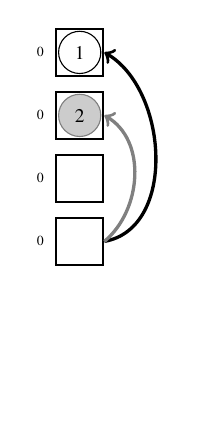
\begin{tikzpicture}
[
textbox/.style={rectangle, draw=white, fill=white,align=center, thick, minimum height=0.5cm},
box1/.style={rectangle, draw=black, fill=white, thick, minimum height=0.6cm, minimum width=2.4cm},
box2/.style={rectangle, draw=black, fill=white, thick, minimum height=0.6cm, minimum width=1.2cm},
box3/.style={rectangle, draw=black, fill=white, thick, minimum height=0.6cm, minimum width=0.6cm},
myarrow1/.style={single arrow, draw=black, fill=black, 
      minimum width = 1mm, single arrow head extend=1mm,
      minimum height=1cm},
myarrow2/.style={single arrow, draw=red, fill=red, 
      minimum width = 1mm, single arrow head extend=1mm,
      minimum height=1.3cm},
myarrow3/.style={single arrow, draw=blue, fill=blue, 
minimum width = 0.09cm, single arrow head extend=0.05cm,
minimum height=0.7cm},
mylabels/.style={text=black, font=\scriptsize},
    every label/.append style={mylabels},
greenball/.style={circle, draw=gray, fill=gray!40, minimum size=1mm},
redball/.style={circle, draw=black, fill=white, minimum size=1mm},
blueball/.style={circle, draw=gray, fill=gray, minimum size=1mm},
]

\node at (0,0) [box3,label={west:$\OLDEST_0$}] (b1)     {};
\node at (0,0) [redball] (g1) {{\scriptsize 1}};
\node at (0,-0.8) [box3,label={west:$\OLDER_0$}] (b2)      {};
\node at (0,-0.8) [greenball] (g2) {{\scriptsize 2}};
\node at (0,-1.6) [box3,label={west:$\OLD_0$}] (b3)               {};
\node at (0,-2.4) [box3,label={west:$\NEW_0$}] (b4)               {};
\node[scale=0.6] at (0.45,-4.3) [textbox] (omap1) {};
\draw [->,black, very thick] (b4.east) to [out=10,in=330] (b1.east) ;
\draw [->,gray,very thick] (b4.east) to [out=40,in=330] (b2.east) ;
\end{tikzpicture}
%\caption{}
\end{subfigure}
\begin{subfigure}[t]{0.3\textwidth} %two
\centering
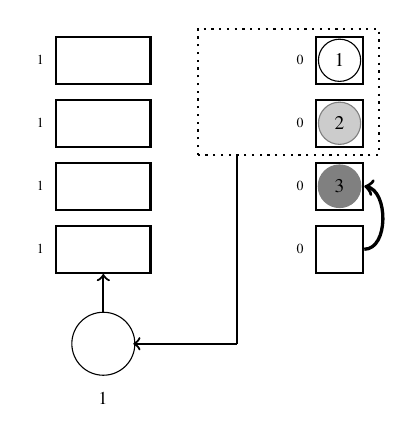
\begin{tikzpicture}
[
textbox/.style={rectangle, draw=white, fill=white,align=center, thick, minimum height=0.5cm},
box1/.style={rectangle, draw=black, fill=white, thick, minimum height=0.6cm, minimum width=2.4cm},
box2/.style={rectangle, draw=black, fill=white, thick, minimum height=0.6cm, minimum width=1.2cm},
box3/.style={rectangle, draw=black, fill=white, thick, minimum height=0.6cm, minimum width=0.6cm},
buf/.style={rectangle, draw=black, fill=white, very thick, minimum height=0.6cm, minimum width=1.2cm},
myarrow1/.style={single arrow, draw=black, fill=black, 
      minimum width = 1mm, single arrow head extend=1mm,
      minimum height=1cm},
myarrow2/.style={single arrow, draw=black, fill=red, 
      minimum width = 1mm, single arrow head extend=1mm,
      minimum height=1.3cm},
myarrow3/.style={single arrow, draw=blue, fill=blue, 
minimum width = 0.09cm, single arrow head extend=0.05cm,
minimum height=0.7cm},
mylabels/.style={text=black, font=\scriptsize},
    every label/.append style={mylabels},
    greenball/.style={circle, draw=gray, fill=gray!40, minimum size=1mm},
redball/.style={circle, draw=black, fill=white, minimum size=1mm},
blueball/.style={circle, draw=gray, fill=gray, minimum size=1mm},
]
\node at (0,0) [box2,label={west:$\OLDEST_1$}] (b10)  {};
\node at (0,-0.8) [box2,label={west:$\OLDER_1$}] (b11)   {};
\node at (0,-1.6) [box2,label={west:$\OLD_1$}] (b12)  {};
\node at (0,-2.4) [box2,label={west:$\NEW_1$}] (b13)  {};


\node[scale=0.6] at (0,-4.3) [textbox] (omap1) {\Large{$\omerge_1$}};
\draw[] (0,-3.6) circle (4mm) node (c2)  {};
\draw[color=black,thick,->]  (0,-3.2) -- (b13) {};
\draw[color=black,thick] (1.7,-1.2) -- (1.7,-3.6) {};
\draw[color=black,thick,->]  (1.7,-3.6) -- (0.38,-3.6) {};
\node at (3,0) [box3,label={west:$\OLDEST_0$}] (b10) {};
\node at (3,-0.8) [box3,label={west:$\OLDER_0$}] (b11)  {};
\node at (3,0) [redball] (g1) {{\scriptsize 1}};
\node at (3,-1.6) [box3,label={west:$\OLD_0$}] (b12)  {};
\node at (3,-0.8) [greenball] (g2) {{\scriptsize 2}};
\node at (3,-2.4) [box3,label={west:$\NEW_0$}] (b13)  {};
\node at (3,-1.6) [blueball] (g2) {{\scriptsize 3}};
\draw[dotted,color=black,thick] (1.2,-1.2) rectangle (3.5,0.4);
\draw [->,color=black!50!black,very thick] (b13.east) to [out=0,in=-10] (b12.east) ;
\end{tikzpicture}
%\caption{}
\end{subfigure}
}
%\caption{\LSDd[$\cdot$]: from $\Sigma$ to DSE.(a) Insertion of the 1st entry happens at $\NEW_0$(Rule 1), making $\NEW_0$ full. Hence it is moved to the empty old index $\OLDEST_0$ (Rule 2, red arrow). The 2nd insertion happens at $\NEW_0$ (Rule 1), making it full again, and is moved to next empty old index $\OLDER_0$ (Rule 2, dark red arrow).(b) During the 3rd insertion, both $\OLDEST_0$ and $\OLDER_0$ are full, so the next $\gamma$ steps of $\Sigma.$\omerge$_1$\ is called (Rule 3), moving entries from $\OLDEST_0\cup \OLDER_1$ (directly or via a buffer) to $\NEW_0$ in the next $2^1$ steps. The 3rd entry is inserted at $\NEW_0$ and moved to $\OLD_0$ (triggering Rule 1 and 2 respectively). (c) During the 4th insertion, $\OLDEST_0$ and $\OLDER_0$ are still full, hence next $\gamma$ steps of $\Sigma.$\omerge (Rule 3) is called. At this point $2^1$ steps of \omerge$_1$\ are done and $\NEW_1$ is full with entries of $\OLDEST_0\cup \OLDER_1$, and is moved to $\OLDEST_1$ (Rule 2, light red arrow). The 4th insertion causes $\NEW_0$ to be full. Hence $\OLD_0$ is moved to $\OLDEST_0$ (red arrow), and $\NEW_0$ is moved to $\OLDER_0$(dark red arrow).}
\label{fig:sddFig}
\end{figure}
	

\begin{figure*}[!h]
\begin{mdframed}
\begin{algorithmic}%[1]
 \Statex \hskip-1.5em$\Gamma \in \{\OneChoice,\TwoChoice, \NlogN \}$
\Statex \hskip-1.5em If $\Gamma = \OneChoice$, $N'= 3{\cdot} 2^i,m_i = \lceil{\frac{2^i}{\log 2^i \log \log 2^i}}\rceil$,  $\forall level\in \{0 \ldots m_i-1\}$ $b_{level} = 3{\cdot}\log 2^i\log \log 2^i$ and $c_{level} = 0$
\Statex \hskip-1.5em If $\Gamma = \NlogN$, $N'= 2^i{\cdot}\log{(2^i+1)}$, $m_i = (i+1)$,   $\forall level\in \{0 \ldots m_i-1\}$ $b_{level} = 2^{level}$ and $c_{level} = 2^{i-level}$
\Statex \hskip-1.5em If $\Gamma = \TwoChoice$, $N'= z{\cdot} 2^i,m_i = \lceil{\frac{2^i}{(\log \log 2^i) (\log \log \log 2^i)^2}}\rceil$,
$\forall level\in \{0 \ldots m_i-1\}$ $b_{level} = z{\cdot}(\log \log 2^i)(\log \log \log 2^i)^2$ and $c_{level} = 0$, $2 \leq z \leq 4$
\Statex
\end{algorithmic}
\underline {{${\sf NEW}_i$ $ \leftrightarrow$ {$\Gamma$.\omerge$_i(K, \sigma; {\sf OLDEST}_{i - 1},{\sf OLDER}_{i - 1})$}}}
\begin{algorithmic}[1]
\item[Client $\leftrightarrow$ Server:] %\tpurp{$\Gamma$ s inside the function should be deleted}
\Statex
\Statex \textcolor{blue}{//** \ \ Phase 1 - Preparing sorted input array\ \   **//}	
\State Client parses $K$ as $(k_{rnd},P)$ \label{fw:parseK}\Comment{all encryptions and decryptions are done with key $k_{rnd}$, $P$ is an array of PRF keys}
%\State Client initializes a tuple called $\pr$ as $(\bot, 0)$ and stores it in local state $\sigma$
\State {Server initializes} arrays \BUF$_1$ of size $3{\cdot}N'$, and \BUF$_2$ of size $N'$ to be empty at Server\label{fw:init}
%\State Perform oblivious sort on $\OLDEST_{i-1}.\Ind \cup \OLDER_{i-1}.\Ind$ in 
%the lexicographic order of keywords; store output in $\BUF_1$ \label{fw:firstsort}
\State Copy $\OLDEST_{i-1}.\Ind \cup \OLDER_{i-1}.\Ind$ to $\BUF_1$; obliviously sort $\BUF_1$ w.r.t. 
 lexicographic order of keywords\label{fw:firstsort}
\State Perform two linear scans (one in reverse and one in correct order) on $\BUF_1$, to add the $rank$ and $n_w$ values to each entry of keyword $w$. The entries now look like $(w,id,op,rank,n_w)$, where $0 \leq rank < n_w$. \label{fw:twoscans}
\State {Linearly scan $\BUF_1$ and pad each keyword-list with dummy elements so that its size is nearest power of 2, hide list lengths by padding total size to $2N'$}\label{fw:pad2}% without leaking the actual list length}
   % \State {$cnt \gets 0$}
   \State {Perform oblivious sort on $\BUF_1$ w.r.t. lexicographic order of the keywords and descending order of the $n_w$ values. Keep first $N'$ elements.}\label{fw:secondsort}
   \Statex
  \Statex \textcolor{blue}{//** \ \ Phase 2---Prepare index elements and prepare keyword counters \ \ **//}	
    \For{each $j = 1 \ldots |\BUF_1|$}\label{fw:loop1start}
    \State Client decrypts $(w,id,op,rank,n_w) \gets \RND.\Dec(k_{rnd},\BUF_1[j])$\label{fw:dec1} %
      \State Client generates {$p \gets^{\$} \{0,1\}^\lambda$}\label{fw:randp}
    \IIf{$rank = 0$}{~Client appends $(\RND.\Enc(k_{rnd},(w,n_w,p)))$ to $\BUF_2$}\label{fw:rank0} %\Comment{\tpurp{I want to do p+1 here}}
    \ElsI{Client appends $(\RND.\Enc(k_{rnd},(\bot,\bot,\bot)))$ to $\BUF_2$}\label{fw:rankN0}
    \State Client generates $((level,pos),\sigma)\gets\texttt{Map}(P[i][3],w,rank,n_w,\sigma)$\label{fw:map} \Comment{$pos=0$ for \OneChoice\ and \TwoChoice\ }
  \State Client writes $(\RND.\Enc(k_{rnd},(w,id,op,level,pos)))$ to \BUF$_{1}[j]$ \label{fw:dec2}
    \EndFor\label{fw:loop1end}
    \Statex
    \Statex \textcolor{blue}{//** \ \ Phase 3---Add dummies\ \ **//}	%\Comment{this phase adds binsize dummy entries per bin}
    \For{$level= 0 \ldots m_i-1$}\label{fw:loop2start}
    \State for every $pos \in\{0 \ldots c_{level}\}$ call Client appends $(\RND.\Enc(k_{rnd},(\bot,\bot,\bot,level,pos)))$ to $\BUF_1$  $b_{level}$ times \label{fw:padbin}
    \EndFor\label{fw:loop2end}
    \Statex
     \Statex \textcolor{blue}{//** \ \ Phase 4---Final placement \ \ **//}	
    \State Perform oblivious sort on $\BUF_1$ w.r.t. the integer values of $(level,pos)$ in ascending order \label{fw:thirdsort}
    \State Linearly scan $\BUF_1$, and tag \textbf{first} $b_{level}$ entries for each $level\in \{0, \ldots, \Sigma.m_i-1\}$ and $pos\in \{0, \ldots, c_{level}\}$ with 1, and with 0 the rest of them (the existing $(level,pos)$ tags are replaced with 0/1 tags, the entries now look like $(w,id,op,x)$, where $x \in \{0,1\}$)\label{fw:0-1tag}
    \State {Perform order preserving oblivious compaction on $\BUF_1$; keep first $N'$ entries; discard the 0/1 tags }\label{fw:compaction}
    \State Perform oblivious sort on $\BUF_2$ w.r.t. the random keys in ascending order; keep first $2^i$ entries; discard random keys\label{fw:buf2sort}
    \State 	Server moves $\BUF_1$ to \NEW$_i.\Ind$  \label{fw:newi} \Comment{elements in each $bin/pos$ is randomly shuffled}
   \For{each $s \in \BUF_2$}\label{fw:dictloopstart}
\State Client decrypts $(w, cnt_w) \gets \RND.\Dec(k_{rnd}, s)$\label{fw:dec3}
\State Client generates $(key,value) \gets \PiBas.\MAP((P[i][3],k_{rnd}),w,cnt_w,1)$ \label{fw:pibasmap}\Comment{parameter 1 is used by the PRF $F$}
\State 	Client writes \NEW$_i.$\Dict[$key$] $\gets value$\label{fw:mapdict}
\EndFor\label{fw:dictloopend}
%\Statex
\State \Return \NEW$_i$
\end{algorithmic}
\end{mdframed}
%\vspace{-1.2em}
\caption{\omerge\ framework of $\Gamma \in \{\OneChoice, \TwoChoice, \NlogN\}$}
\label{alg:framework}
\vspace{+1.3em}
\end{figure*}

\smallskip\noindent\textbf{Phases of {\omerge} framework.}\label{sec:oblivious_merge}
%\todo{5.Clearly explain that SDd[] works only with 1C/2C/NlogN and not scheme-agnostic}
Now we will present our \omerge\ framework that 
ensures properties \textsf{{(P1)}}, \textsf{{(P2)}}, 
and \textsf{{(P3)}} for the static 
SE scheme $\Gamma$ $\in$ $\{\OneChoice,$ $\TwoChoice,$ $\NlogN\}$, in detail. 
%\todo{7.Clarify which scheme targets which storage and which metrices} 
Similar to \SDa, we have \LSDd[\OneChoice] and \LSDd[\TwoChoice] (suitable for HDDs), as well as \LSDd[\NlogN] (compatible with both HDDs and SSDs).
The corresponding is presented in Figure \ref{alg:framework}. 
Some of the steps are not necessary for all the schemes in  $\{\OneChoice,$ $\TwoChoice,$ $\NlogN\}$, 
but we needed them in order to create the general \omerge\ framework. 
\new{Towards the end of this section we discuss some optimization specific to each scheme.  Here, we also would like to point out, the temporary client storage cost is upper bounded by the update cost (e.g. $\bO(\log^2 N)$ for \LSDd[\OneChoice]), while the permanent client storage is constant. }

The high level idea is, instead of moving elements directly from 
$\OLDER_{i-1}.\Ind \cup \OLDEST_{i-1}.\Ind$ to $\NEW_i.\Ind$ 
(using oblivious dictionaries, as done in \cite{SDa}), 
move them to a buffer $\BUF_1$ first. This step will ensure 
property \textsf{{(P2)}}. Then with oblivious operations, re-order the entries of $\BUF_1$ to 
satisfy the I/O efficiency requirements of scheme $\Gamma$, 
and then move $\BUF_1$ to $\NEW_i$.\Ind. {This step and the previous step 
together ensure property \textsf{{(P1)}}. 
{The buffer, $\BUF_2$, is used to create  
the keyword dictionary, $\NEW_i.\Dict$}, in an oblivious fashion as well.
The references to $\OLDER_{i-1}$ and $\OLDEST_{i-1}$ are passed as parameters to the \omerge$_i$ protocol.
Each \omerge$_i$ instance runs in four phases. Below we discuss the four phases in detail. Refer to Figure \ref{alg:framework} for the pseudocode. 
If a step in the pseudocode does not mention who is performing it (i.e. Client or Server), it means multiple rounds of communication happens between the client and the server to perform that step.}
\neww{Finally, at the end of $2^i$ calls to \omerge$_i$ it returns $\NEW_i$ (i.e. $\NEW_i.\Ind$  and $\NEW_i.\Dict$). }

\noindent\textbf{\underline{Phase 1.}} %In this phase 
\new{Entries of $\OLDER_{i-1}.\Ind \cup \OLDEST_{i-1}.\Ind$ are 
first copied (not moved) to $\BUF_1$.} Next, $\BUF_1$ is 
obliviously sorted based on the lexicographic order 
of the keywords (line \ref{fw:firstsort}). \new{The sort places 
entries for the same keyword adjacent to each other in $\BUF_1$, 
and the dummy entries are placed at the end. Each entry of 
$\BUF_1$ is then assigned a $rank$} and an $n_w$ value via two 
linear scans (line \ref{fw:twoscans}). Next, each keyword-list 
in $\BUF_1$ is padded to make their lengths to be nearest power of 2 
(line \ref{fw:pad2}). Another oblivious sort is performed on $\BUF_1$, 
based on the lexicographic order of the keywords, as well as descending 
order of the $n_w$ values   (line \ref{fw:secondsort}). This sort places 
same keyword entries adjacent to each other and entries with higher 
$n_w$ values are placed before entries with lower $n_w$ values in $\BUF_1$.

We provide a more detailed pseudocode for lines \ref{fw:twoscans} and \ref{fw:pad2} in the extended version.

\noindent\textbf{\underline{Phase 2.}} This phase prepares the elements in $\BUF_1$ for 
$\NEW_i.\Ind$ by adding proper position tags to them 
(lines \ref{fw:map}-\ref{fw:dec2}), and prepares $\BUF_2$ 
for creating $\NEW_i.\Dict$ (lines \ref{fw:randp}-\ref{fw:rankN0}). 
For every entry in $\BUF_1$\ $(w,id,op,rank,n_w)$ an entry is appended to 
$\BUF_2$. When $rank=0$, a real entry $(w,n_w,p)$ 
is appended to $\BUF_2$. 
\new{In all other cases a dummy entry $(\bot,\bot,\bot)$ is added (line \ref{fw:rankN0})
(because we can neither reveal the length of each keyword-list, nor the number of unique keywords). }
Here, $p$ is a uniformly generated random key of $\lambda$ bit.

The $\MAP$ function of $\Gamma$ is called for each 
entry of $\BUF_1$,  which %with appropriate arguments, which 
returns a pair $(level,pos)$. 

 \new{For every $\Gamma \in \{\OneChoice,\TwoChoice,\NlogN\}$ the pseudocode for the corresponding $\MAP$ function is provided in the extended version}.
For $\OneChoice$ and $\TwoChoice$ the value of $level$ indicates  
the bin number assigned to this entry, and $pos$ is 0 by default. 
Whereas, for \NlogN\ scheme 
$level(\in \{0,\ldots,i\})$ indicates the array level,
and position indicates the position $pos (\in \{0,\ldots, (2^{i-level}\minus1)\})$ in the array level.
The encrypted entry $(w,id,op,level,pos)$ replaces the existing 
$(w,id,op,rank,n_w)$ entry in $\BUF_1$. 

\noindent\textbf{\underline{Phase 3.}}
This phase adds dummy elements 
(lines \ref{fw:loop2start}-\ref{fw:loop2end}) to $\BUF_1$, beacuse  
every bin needs to be filled up to their maximum capacity. 
For \OneChoice\ and \TwoChoice\, if bin size is $b_i$ then 
the dummy element $(\bot,\bot,\bot,bin,0)$ is appended to $\BUF_1$ $b_i$ times. 
This step is repeated for each bin number $bin$.  
For \NlogN\ scheme, array level $k$ contains $2^{i-k}$ 
lists of size $2^k$.
Hence, the dummy entry $(\bot,\bot,\bot,k,pos)$ 
is appended $2^k$ times for each $pos \in \{0,\ldots, (2^{i-k}-1)\}$.
This step is repeated for levels $k \in \{0, \ldots, i\}$. 
\new{We add a total of $3{\cdot}2^i$ dummy elements for \OneChoice\ and 
\TwoChoice\, and $2^i{\cdot}\log {2^i}$ dummy elements for \NlogN.
The goal is to add dummy entries for every vacant positions of the bins/levels.
But we want} to hide the number of real elements {in each bin/level, and so 
 the number of dummy elements we add is equal to the index size.
Extra dummy elements are discarded in Phase 4.}
\noindent\textbf{\underline{Phase 4.}} 
This phase consists of few steps. 
%(lines \ref{fw:thirdsort}-\ref{fw:dictloopend}). 
%Each of them can be de-amortized.
The oblivious sort on line \ref{fw:thirdsort} 
sorts $\BUF_1$ based on $(level,pos)$ values.
Dummy elements come last, as usual.
But now we have more elements assigned to each bin/level than their capacity. 
Hence, with a linear scan (line \ref{fw:0-1tag}) 
unnecessary elements are tagged with a 0;
and the entries to be kept are tagged with a 1. 
%(red and blue tags respectively in Figure \ref{fig:buf1f}).
This tag replaces the existing $(level,pos)$ tags.
Next, an order preserving oblivious compaction (line \ref{fw:compaction}) is 
performed so that all elements tagged with 0 come at the tail of the output and 
can be discarded altogether. We use 
another round of oblivious bucket sort (which is order preserving) for the compaction. 
%The 0/1-bit tags are removed from each entry at the end.
%Next, the entries %at the beginning that were tagged with 
%1-bit in 
$\NEW_i.\Ind$ is created with the remaining entries of $\BUF_1$ (line \ref{fw:newi}). 
$\BUF_2$ is also obliviously sorted (line \ref{fw:buf2sort}) based on 
the random keys in ascending order. 
The dummy entries with $p=\bot$ will be placed at the end of the sorted buffer.
There can be at most $2^i$ entries such that $p \neq \bot$, as 
there can be at most $2^i$ distinct keywords at index level $i$.
Hence, the first $2^i$ elements are used to 
create $\NEW_i.\Dict$ (lines \ref{fw:dictloopstart}-\ref{fw:dictloopend}).

\smallskip\noindent\textbf{Locality-aware \LSDd$[\cdot]$.}
\new{The search-\emph{locality} and search-\emph{read efficiency} of \LSDd[$\Gamma$]
depends on the same of the static SE scheme $\Gamma$. For both \emph{locality} 
and \emph{read efficiency}, a $\log N$ factor is added 
due to querying $3{\cdot}\log N$ dictionaries and calling 
$\Gamma.\Search$ on $3{\cdot}\log N$ indexes (for \OLDEST, \OLDER, and \OLD). 
For example, \OneChoice\ offers $\bO(1)$ \emph{locality} 
and $\bO(\log N \log \log N)$ \emph{read efficiency}, whereas \LSDd[\OneChoice] offers 
$\bO(\log N)$ \emph{locality} and $\bO(\log N \log \log N +\log N)$ \emph{read efficiency}. 
Similarly, \LSDd[\NlogN] offers $\bO(\log N)$ \emph{locality} and $\bO(\log N)$ \emph{read efficiency}, 
as opposed to optimal \emph{locality} and \emph{read-efficiency} that is offered by \NlogN.} 

\smallskip\noindent\textbf{Page-efficient \LSDd{[.]}.}
We can instantiate \LSDd[$\cdot$] on SSDs with static page efficient schemes 
like \NlogN\  \cite{onechoice} and its variations i.e. \Ns\ \cite{Demertzis17}. 
The \emph{page efficiency} of \LSDd[\NlogN] is $\bO(\log N)$ vs. the 
optimal \emph{page efficiency} offered by \NlogN, whereas 
for \LSDd[\Ns] \emph{page efficiency} is $\bO(N^{\frac{1}{s}}/p+\log N)$. 

\smallskip\noindent\textbf{Security and efficiency.} We formally state and prove the security of \LSDd[$\Gamma$] 
(for $\Gamma \in \{\OneChoice,\TwoChoice,\NlogN\}$) in the extended version. The security of \SDd[\PiBas] is already proven in \cite{SDa}. 
We prove also that when we instantiate a locality-aware static scheme $\Gamma$ with \LSDd[$\cdot$], it retains its space overhead, but for \emph{locality} and \emph{read-efficiency} an additional $3\log N$ factor is introduced as $3\log N$ indexes are queried (similar proof for the \emph{page-efficient} \LSDd[$\cdot$] transformation can be proven)---see the extended version. 

\smallskip\noindent\textbf{\OneChoice\ Optimization.} 
In \OneChoice\ scheme we do not need to make the keyword-lists' sizes to be of power of 2. 
We also do not need to store the larger keyword-lists into the bins before the 
smaller lists. Hence the lines \ref{fw:pad2} and \ref{fw:secondsort} 
in Figure \ref{alg:framework} are not required for \OneChoice.
%In Figure \ref{alg:sdd1C} those two lines are omitted.
The two linear scans that add $rank$ and
$n_w$ values to each entry can be also removed (line \ref{fw:twoscans}). 
This is because, after the first oblivious sort
the entries for the same keyword are all placed together in adjacent locations. In Phase 2, with the help of a single counter 
%($cnt$ variable in 
%line \ref{sdd1c:counter} in Figure \ref{alg:sdd1C}), 
one can count how many occurrences of 
a particular keyword has been seen. %(and $\BUF_2$ can be updated accordingly).
Based on this counter value $\BUF_2$ can be updated accordingly.
The same counter value can be used in $\OneChoice.\MAP$ function to compute 
the bin numbers.% (line \ref{sdd1c:map} in Figure \ref{alg:sdd1C}).
The counter needs to be reset to 0 every time a new keyword is observed. We provide the optimized pseudocode for  \OneChoice.\omerge\ in the extended version. 


\smallskip\noindent\textbf{\NlogN\ Optimization.} 
%\paragraph{{\textbf{\NlogN\ Optimization.}}}
Here the order of storing lists does not matter.
Thus, the second oblivious sort (line \ref{fw:secondsort}) can be omitted in Phase 1 for the \NlogN\ scheme.
This can be further optimized 
by storing only $s$ evenly distributed arrays, 
instead of $\ell=\log N+1$ arrays, which 
is essentially the \textsf{Ns} scheme.

\smallskip\noindent\textbf{\TwoChoice\ Optimization.} 
For \TwoChoice\ scheme, the client needs to maintain a map to remember which bin has how many entries.
This is because, placement of a keyword-list into a superbin 
depends on how full the superbin is. 
There are can be maximum of $m = \lceil{{N}/{\log\log N (\log \log \log N)^2}}\rceil$  
bins. But in \LSDd\ there are $\log N$
index levels. Hence, to maintain this information the required  
client storage is $\bO(m{\cdot}\log N)$.
To achieve a constant client storage, this map can 
be stored at the server in oblivious maps (see section \ref{sec:prelim}).

\smallskip\noindent\textbf{Update cost.}
The \omerge\ framework shown in Figure \ref{alg:framework} mainly consists of three types of building blocks: bucket oblivious sorts, 
basic \algorithmicfor\ loops and linear scans.
Linear scans are realized with basic \algorithmicfor\ loops. 
The costliest operation among these is the bucket oblivious sort \cite{bucketSort}, 
which can be decomposed into $N$ steps of $\bO(\log N)$ work per step, 
assuming an index contains at most $N$ entries 
(recall the $i$th index contains $2^i$ elements).
In the extended version we explain how to 
deamortize the bucket oblivious sort in detail. 
Even the \algorithmicfor\ loops can be executed for $\bO(\log N)$ 
iterations during a particular call of \omerge$_i$ (for the $i$th index). Overall, an \omerge$_{i}$ protocol can be decomposed into $N$ steps of at most $\bO(\log N)$ work per step. There are $\log N$ levels in \LSDd[${\cdot}$]. Hence, the \emph{worst case} update cost is $\bO(\log^2 N)$ for \LSDd[\OneChoice], and \LSDd[\TwoChoice]. For \LSDd[\NlogN] the update cost is $\bO(\log^3 N)$, because it has at most $\log N$ levels per index.
%\section{Experimental Evaluation}\label{sec:eval}

\begin{figure}[t]
\small
 \centering\begin{tabular}{|c|c|c|} 
\hline
\multirow{2}{*}{\parbox{2cm}{\centering Scheme}} & \multirow{2}{*}{\parbox{2cm}{\centering Size(GB) for $|DB|=2^{23}$}} & \multirow{2}{*}{\parbox{2cm}{\centering Size(GB) for $|DB|=2^{26}$}} \\ & & \\
\hline 
 \LSDd[\NlogN] & 49 & 436 \\
 \LSDd[\OneChoice] & 7.5 & 60\\
 \SDd[\PiBas] & 5 & 40 \\
\hline
\end{tabular}
%\end{adjustbox}
\caption{Needed storage for a dataset and encrypted index.}
\label{table:storage}
\end{figure} 
%\tgreen{ I/O matters for in memory too.}
%\tgreen{ Repository link of the code}
%\tgreen{why SDd[Pibas] better that SDa[PiBas] in some cases}.
We report the performance of our schemes and compare them with previous state-of-the-art works. 
\begin{figure*}[ht]
	\centering
	\begin{subfigure}[t]{0.24\linewidth}
		\includegraphics[width=\textwidth]{chapters/iodse/figures/Search-Comp-DBSize10M-ResultSizeVar-32B-NoCache.eps}
		\vspace{-0.8cm}
		\caption{}
	\end{subfigure}
 	\begin{subfigure}[t]{0.24\linewidth}
		\includegraphics[width=\textwidth]{chapters/iodse/figures/Search-Comp-DBSize10M-ResultSizeVar-32B-NoCache-SSD.eps}
		\vspace{-0.8cm}
		\caption{}
	\end{subfigure}
		\begin{subfigure}[t]{0.24\linewidth}
		\includegraphics[width=\textwidth]{chapters/iodse/figures/Search-Comp-DBSizeVar-ResultSize1000.eps}
		\vspace{-.8cm}
		\caption{}
	\end{subfigure}
 	\begin{subfigure}[t]{0.24\linewidth}
		\includegraphics[width=\textwidth]{chapters/iodse/figures/Search-Comp-DBSizeVar-ResultSize1000-SSD.eps}
		\vspace{-.8cm}
		\caption{}
	\end{subfigure}%

	\vspace{-.3cm}
	\caption{Search computation time for $|{DB}|=2^{23}$ and variable result size for (a) $|block|=32$B in (a) HDD, (b) SSD. Search computation time for variable database size and $n_w=1K$ in (c) HDD, (d) SSD.}
	\label{fig:search-var}
	%\vspace{-.5em}
\end{figure*}

\begin{figure*}[ht]
	\centering
	\begin{subfigure}[t]{0.24\linewidth}
		\includegraphics[width=\textwidth]{chapters/iodse/figures/Search-Comp-DBSize10M-ResultSizeVar-512B-NoCache.eps}
		\vspace{-.8cm}
		\caption{}
	\end{subfigure}%
 	\begin{subfigure}[t]{0.24\linewidth}
		\includegraphics[width=\textwidth]{chapters/iodse/figures/Search-Comp-DBSizeVar-ResultSize10000.eps}
		\vspace{-.8cm}
		\caption{}
	\end{subfigure}~
		\begin{subfigure}[t]{0.24\linewidth}
		\includegraphics[width=\textwidth]{chapters/iodse/figures/Search-Comp-DBSizeVar-ResultSize10000-SSD.eps}
		\vspace{-.8cm}
		\caption{}
	\end{subfigure}~
  \begin{subfigure}[t]{0.24\linewidth}
		\includegraphics[width=\textwidth]{chapters/iodse/figures/SearchTime-WAN2.eps}
		\vspace{-0.6cm}
	\end{subfigure}\\
	%\vspace{-.3cm}
	\caption{Search computation time for $|{DB}|=2^{23}$ and variable result size for (a)  $|block|=512$B in HDD. Search computation time for variable database size and $n_w=10K$ in (b) HDD, (c) SSD. (d) Search computation time for $|{DB}|=2^{23}$, $|block|=32$B in HDD and variable result size for WAN machines with 24.7ms network delay and 2.5Gbps bandwidth.}
	\label{app-fig:search-var2}
% 	\vspace{-.3cm}
\end{figure*}

We implemented \SDa[\OneChoice], \SDa[\TwoChoice], \SDa[\NlogN], \SDa[\textsf{\Ns}], \LSDd[\OneChoice] and \LSDd[\sN] with approximately 
$31K$ lines in C++. 
We used  OpenSSL-AES~\cite{openssl} 
PRF evaluation and semantically secure encryption. 
We also used Oblivious MAP of~\cite{SDa} {for the \SDd[\PiBas] implementation}, 
and merge-sort as the last step in the implementation of 
bucket oblivious sort~\cite{bucketSort}. We ran our experiments on a machine with
%\tgreen{highlight single core implementation} 
Intel Xeon E-2174G 3.8GHz processor,  128GB  RAM, 1TB SSD, and 5TB HDD running 
Ubuntu 20.04 LTS (limited to one CPU core for our experiments). 
%All schemes were instantiated on a single machine, \tpurp{although communication time between a client and a server can be easily simulated}. 
Our code is available online.\footnote{https://github.com/jgharehchamani/DSE-with-IO-Locality} %\tgreen{SSD/HDD speeds/ RAM speed DDRx ?}







\begin{figure*}[ht]
	\centering
	\begin{subfigure}[t]{0.24\linewidth}
		\includegraphics[width=\textwidth]{chapters/iodse/figures/Search-Comp-DBSize10M-ResultSizeVar-32B-NoCache-2.eps}
		\vspace{-0.8cm}
		\caption{}
	\end{subfigure}
	\begin{subfigure}[t]{0.24\linewidth}
		\includegraphics[width=\textwidth]{chapters/iodse/figures/Search-Comp-DBSize10M-ResultSizeVar-512B-NoCache-2.eps}
		\vspace{-.8cm}
		\caption{}
	\end{subfigure}%
		\begin{subfigure}[t]{0.24\linewidth}
		\includegraphics[width=\textwidth]{chapters/iodse/figures/Search-Comp-DBSizeVar-ResultSize1000-2.eps}
		\vspace{-.8cm}
		\caption{}
	\end{subfigure}~
 	\begin{subfigure}[t]{0.24\linewidth}
		\includegraphics[width=\textwidth]{chapters/iodse/figures/Search-Comp-DBSizeVar-ResultSize10000-2.eps}
		\vspace{-.8cm}
		\caption{}
	\end{subfigure}~\\
% 	\vspace{-.4cm}
% 	\caption{Search computation time for $|{DB}|=2^{23}$ and variable result size for: (a) $|block|=32$B in HDD, (a) $|block|=32$B in SSD, (c) $|block|=512$B in HDD.}
% 	\label{fig:search-var-block}
	\vspace{-.2cm}
% \end{figure*}

% \begin{figure*}[ht]
% 	\centering
	\begin{subfigure}[t]{0.24\linewidth}
		\includegraphics[width=\textwidth]{chapters/iodse/figures/Search-Comp-DBSize10M-ResultSizeVar-32B-NoCache-SSD-2.eps}
		\vspace{-0.8cm}
		\caption{}
	\end{subfigure}
	\begin{subfigure}[t]{0.24\linewidth}
		\includegraphics[width=\textwidth]{chapters/iodse/figures/Search-Comp-DBSizeVar-ResultSize1000-SSD-2.eps}
		\vspace{-.8cm}
		\caption{}
	\end{subfigure}%
		\begin{subfigure}[t]{0.24\linewidth}
		\includegraphics[width=\textwidth]{chapters/iodse/figures/Search-Comp-DBSizeVar-ResultSize10000-SSD-2.eps}
		\vspace{-.8cm}
		\caption{}
	\end{subfigure}~
	\vspace{-.3cm}
	\caption{Search computation time for $|{DB}|=2^{23}$ and variable result size for (a) $|block|=32$B in HDD, (b) $|block|=512$B in HDD. Search computation time for variable database size and (c) $n_w=1K$ in HDD, (d) $n_w=10K$ in HDD. Search computation time for $|{DB}|=2^{23}$ and variable result size for (e) $|block|=32$B in SSD. Search computation time for variable database size and (f) $n_w=1K$ in SSD, (g) $n_w=10K$ in SSD.}
	\label{app-fig:search-var}
% 	\vspace{-.3cm}
\end{figure*}

\begin{figure}[!ht]
	\centering
	\begin{subfigure}[t]{0.49\linewidth}
		\includegraphics[width=\textwidth]{chapters/iodse/figures/Search-SDA.eps}
		\vspace{-0.8cm}
		\caption{}
	\end{subfigure}
	\begin{subfigure}[t]{0.49\linewidth}
		\includegraphics[width=\textwidth]{chapters/iodse/figures/Search-SDA-SSD.eps}
		\vspace{-.8cm}
		\caption{}
	\end{subfigure}%
	\vspace{-.3cm}
	\caption{Search computation time for $|{DB}|=2^{23}$, variable result size, and $|block|=32$B for different \NlogN settings in (a) amortized HDD, (b) amortized SSD.}
	\label{app-fig:search-var-amor-deamor}
% 	\vspace{-.3cm}
\end{figure}

% \begin{figure*}[ht]
% 	\centering
% 	\begin{subfigure}[t]{0.33\linewidth}
% 		\includegraphics[width=\textwidth]{figures/Search-Comp-DBSize10M-ResultSizeVar-32B-NoCache.eps}
% % 		\vspace{-0.8cm}
% 		\caption{}
% 	\end{subfigure}
% 	\begin{subfigure}[t]{0.33\linewidth}
% 		\includegraphics[width=\textwidth]{figures/Search-Comp-DBSize10M-ResultSizeVar-32B-NoCache-SSD.eps}
% % 		\vspace{-.8cm}
% 		\caption{}
% 	\end{subfigure}%
% 		\begin{subfigure}[t]{0.33\linewidth}
% 		\includegraphics[width=\textwidth]{figures/Search-Comp-DBSize10M-ResultSizeVar-512B-NoCache.eps}
% % 		\vspace{-.8cm}
% 		\caption{}
% 	\end{subfigure}~
% % 	\vspace{-.4cm}
% 	\caption{Search computation time for $|{DB}|=2^{23}$ and variable result size for: (a) $|block|=32$B in HDD, (a) $|block|=32$B in SSD, (c) $|block|=512$B in HDD.}
% 	\label{fig:search-var-block}
% % 	\vspace{-.3cm}
% \end{figure*}

% \begin{figure*}[ht]
% 	\centering
% 	\begin{subfigure}[t]{0.24\linewidth}
% 		\includegraphics[width=\textwidth]{figures/Search-Comp-DBSizeVar-ResultSize1000.eps}
% % 		\vspace{-0.8cm}
% 		\caption{}
% 	\end{subfigure}
% 	\begin{subfigure}[t]{0.24\linewidth}
% 		\includegraphics[width=\textwidth]{figures/Search-Comp-DBSizeVar-ResultSize1000-SSD.eps}
% % 		\vspace{-.8cm}
% 		\caption{}
% 	\end{subfigure}%
% 		\begin{subfigure}[t]{0.24\linewidth}
% 		\includegraphics[width=\textwidth]{figures/Search-Comp-DBSizeVar-ResultSize10000.eps}
% % 		\vspace{-.8cm}
% 		\caption{}
% 	\end{subfigure}~
% 	\begin{subfigure}[t]{0.24\linewidth}
% 		\includegraphics[width=\textwidth]{figures/Search-Comp-DBSizeVar-ResultSize10000-SSD.eps}
% % 		\vspace{-.8cm}
% 		\caption{}
% 	\end{subfigure}%
% % 	\vspace{-.4cm}
% 	\caption{Search computation time for variable database size and (a) $|result|=1K$ in HDD, (b) $|result|=1K$ in SSD, (c) $|result|=10K$ in HDD, (d) $|result|=10K$ in SSD}
% 	\label{fig:search-var-db}
% % 	\vspace{-.3cm}
% \end{figure*}
We focus on the computation time for Search and Update queries and measure these parameters for variable-size synthetic datasets with $|{DB}| = 2^{11}$-$2^{26}$ records randomly shuffled before insertion, each time setting the total number of distinct keywords $|W|$ to $|{DB}|/100$. Likewise, we report results for varying result size $n_w$ between $10$ and $5M$ documents. We also consider two block sizes: 32B and 512B. %\tgreen{why this two blocksize only} 
%To demonstrate the importance of I/O in environment with limited available memory, we perform the experiments in a cold cache environment. 
\neww{To highlight the significance of I/O in a memory-constrained environment, we conduct our experiments in a cold cache setting, but we also provide two sets of experiments to show the effect of cache on the performance of our schemes. In the first one, we keep the different ratios of datasets in the memory (as cache) and respond to the queries for those encrypted data from memory. Note that we normalize the cache for each scheme. In other words, we fix the cache size and load as much as data we can in that memory.}
% Clearly, schemes with more storage need can benefit less from the cache. 
\neww{In the second, we assume there are many users ($200$ for HDD and $75$ for SSD) each of which has her own dataset with size $2^{20}$ and they execute their own search queries randomly when the cache in the system is enabled.}
%To demonstrate the effect of locality on the execution time, we disabled the hard-disk caching mechanism using \path{hdparm} and \path{nvme} commands and dropped the operating system's cache before each disk access by writing to \path{/proc/sys/vm/drop_caches}. 

Experiments were repeated five times, and the average result is reported. \neww{We also provide a comparison between the needed storage on the server for each de-amortized scheme in Figure~\ref{table:storage} for a dataset with $|block|=32B$ where $|DB|=2^{23}$ and $|DB|=2^{26}$. Note that we focus on small client storage schemes. Therefore, client storage is constant.}




%
% In addition to computation time, we compared the used storage of our schemes with the previous works (see Table~\ref{table:storage}). We measured this for a dataset with size $2^{23}-1$ (to fill all levels of the amortized schemes) and a block size of 32 bytes. For \SDd[\PiBas] scheme, the OMAP storage is also counted in the needed storage.
We also repeated the search experiments on a real dataset  consisting of $22$ attributes and $6,123,276$ records of reported crime incidents in Chicago~\cite{crimes}. We used two different attributes, containing 34 and 170 distinct keywords, respectively, and keyword frequency ranging from $1$ record to $1,631,721$ records.
\neww{Finally, we simulated the search and update time of our schemes when run over WAN with 24.7ms delay and 2.5Gbps bandwidth on AWS (between two machines on Ireland and Frankfurt zones).}

\subsection{Search Performance}
Our first set of experiments focuses on search performance and we demonstrate the impact of variable data block sizes, variable result sizes, variable database sizes, \neww{and cache size on all our schemes and compare them with \SDa[\PiBas]~\cite{SDa} and \SDd[\PiBas]~\cite{SDa}. We do not provide the big-block experiments for SSD due to disk space limits.}
%\todo{15. Explain if experimental results can be reproduced in more realistic settings}

\smallskip\noindent\textbf{Variable Block and Result Sizes.} Figure~\ref{fig:search-var} (a,b) and  Figure~\ref{app-fig:search-var2} (a) show the search computation time of a dataset with size $2^{23}$  $|block|=32$B as the result size $n_w$ changes. Similar results for our amortized schemes are in Figure~\ref{app-fig:search-var} (a),(b),(e).

% (results for $|block|=512$B are in Appendices~\ref{append:perf-amort} and~\ref{append:perf-deamort}. 
% a
% nd \ref{}). 
The  conclusions from these experiments are: 
(i) As expected, \SDa[\PiBas] and \SDd[\PiBas]\ have the worst performance among all other schemes for large result sizes due to their poor locality (in HDD) and page efficiency (in SSD). They need to change the position of the hard-drive head or bring different pages of the results, stored at random locations, which leads to significant {slowdown}. (ii) The \SDa[\NlogN]\ and \LSDd[\NlogN] schemes achieve the best performance in the amortized and de-amortized setting, at the cost of extra storage. The number of indexes searched in \LSDd[$\cdot$] is three times than that of \SDa[$\cdot$], hence the search time of \LSDd[\NlogN] is slightly 
more than \SDa[\NlogN]. (iii) \SDa[\TwoChoice] performs better than \SDa[\OneChoice] for small result sizes. However, their performance is the same for result sizes more than the bin's threshold, since, after the threshold entries are stored using \SDa[\OneChoice] (therefore we ignored this scheme in SSD experiments). (iv) The execution time for \SDa[\OneChoice] for result sizes bigger than $10^5$ remains approximately constant, as at this point the database is read in its entirety (i.e. all bins contain results). (v) When the block size is increased from 32B to 512B, 
the search time of all schemes increases, but the gap between \SDa[\TwoChoice]/\SDa[\OneChoice] and \SDa[\PiBas] decreases. This is due to the increase in the volume of the data read for blocks of size 512B, which becomes the dominant factor in the performance. (vi) Amortized and de-amortized versions of \PiBas, \OneChoice, and \NlogN\ have similar performance.
Finally, all our schemes have excellent performance in practice. E.g., \SDa[\OneChoice] and \SDa[\NlogN]/\LSDd[\NlogN] are up to three orders of magnitude faster than \SDa[\PiBas]/\SDd[\PiBas] (for $|n_w|=10^5$ and $|DB|=2^{23}$ \SDa[\OneChoice], \SDa[\NlogN], and \SDa[\PiBas] take 16s, 0.8s, and 903s respectively).

% \todo{26.Explain how communication cost and latency is improved in our scheme}
% \todo{27.Explain Why fully disabling HDD caching the right evaluation point }
% \todo{28. Experiments with client and server on separate machines}
% \todo{33. Provide sizes of the databases in bytes(NDSS)}
% \todo{34.”Real impact of HDD/SDD speeds unclear”(NDSS)}
% \todo{37. Evaluate performance on a larger database(NDSS)}



% \subsection{\SDa\textup{[\NlogN]} Update Experiment} \label{append:sda-nlogn}


\smallskip\noindent\textbf{Variable Database Size.} Figures~\ref{fig:search-var} (c,d) and Figures~\ref{app-fig:search-var2} (b),(c) show the effect of database size on search computation. (Results for the amortized schemes are in Figures~\ref{app-fig:search-var2} (c),(d),(f),(g)). For small blocks it varies search time for variable database sizes between $2^{11}-2^{26}$ and for result size $n_w$=1K in HDD and SSD. As the figures show, the search time of all schemes increases as the database size increases, because of the added levels in the data structures. However, all our schemes are significantly faster than \SDa[\PiBas] and \SDd[\PiBas]. For instance, the amortized schemes \SDa[\OneChoice], \SDa[\TwoChoice], and \SDa[\NlogN] are faster than \SDa[\PiBas] by $2-136\times$, $5-159\times$, and $4-209\times$ respectively. Also, the de-amortized schemes, \LSDd[\OneChoice] and \LSDd[\NlogN] are faster than \SDd[PiBAS] by $2-58\times$ and $3-70\times$ respectively.

\begin{figure*}[ht]
	\centering
	\begin{subfigure}[t]{0.24\linewidth}
		\includegraphics[width=\textwidth]{figures/Cache-25.eps}
		\vspace{-.8cm}
		\caption{}
	\end{subfigure}%
		\begin{subfigure}[t]{0.24\linewidth}
		\includegraphics[width=\textwidth]{figures/Cache-50.eps}
		\vspace{-.8cm}
		\caption{}
	\end{subfigure}~
 	\begin{subfigure}[t]{0.24\linewidth}
		\includegraphics[width=\textwidth]{figures/Cache-75.eps}
		\vspace{-.8cm}
		\caption{}
	\end{subfigure}
 	\begin{subfigure}[t]{0.24\linewidth}
		\includegraphics[width=\textwidth]{figures/Cache-100.eps}
		\vspace{-0.8cm}
		\caption{}
	\end{subfigure}~\\
	\vspace{-.4cm}
	\caption{Search computation time for $|{DB}|=2^{23}$ and variable result size for $|block|=32$B in HDD, (a) 25\% Caching, (b) 50\% Caching, (c) 75\% Caching, (d) 100\% Caching.}
	\label{fig:cache-hdd}
	%\vspace{-.2cm}
\end{figure*}
\begin{figure*}[ht]
	\centering
	\begin{subfigure}[t]{0.24\linewidth}
		\includegraphics[width=\textwidth]{chapters/iodse/figures/Cache-25-SSD.eps}
		\vspace{-.8cm}
		\caption{}
	\end{subfigure}%
		\begin{subfigure}[t]{0.24\linewidth}
		\includegraphics[width=\textwidth]{chapters/iodse/figures/Cache-50-SSD.eps}
		\vspace{-.8cm}
		\caption{}
	\end{subfigure}~
 	\begin{subfigure}[t]{0.24\linewidth}
		\includegraphics[width=\textwidth]{chapters/iodse/figures/Cache-75-SSD.eps}
		\vspace{-.8cm}
		\caption{}
	\end{subfigure}
    \begin{subfigure}[t]{0.24\linewidth}
		\includegraphics[width=\textwidth]{chapters/iodse/figures/Cache-100.eps}
		\vspace{-0.8cm}
		\caption{}
	\end{subfigure}~\\
	\vspace{-.4cm}
	\caption{Search computation time for $|{DB}|=2^{23}$ and variable result size for $|block|=32$B in SSD, (a) 25\% Caching, (b) 50\% Caching, (c) 75\% Caching, (d) 100\% Caching.}
	\label{fig:cache-ssd}
	%\vspace{-.2cm}
\end{figure*}

\begin{figure}[ht]
	\centering
	\begin{subfigure}[t]{0.48\linewidth}
		\includegraphics[width=\textwidth]{chapters/iodse/figures/email-hdd.eps}
		\vspace{-0.6cm}
		\caption{}
	\end{subfigure}
 \begin{subfigure}[t]{0.48\linewidth}
		\includegraphics[width=\textwidth]{chapters/iodse/figures/email-ssd.eps}
		\vspace{-0.6cm}
		\caption{}
	\end{subfigure}
	\vspace{-.3cm}
	\caption{Search computation time for $|{DB}|=2^{20}$ for each user and variable result size for $|block|=32$B with caching enabled in (a) HDD where 200 users exist in the system (b) SSD where 75 users exist in the system}
	\label{fig:email}
% 	\vspace{-.3cm}
\end{figure}






\smallskip\noindent\textbf{Effect of the value of \emph{s} on \SDa[\NlogN] and \LSDd[\NlogN].} The previous experiments showed that our \NlogN-based schemes have the best performance at a cost 
of more (i.e. $\log N$ times) storage.
% \footnote{For the vanilla \NlogN\ scheme the value of $s$ is $\log N$}. 
However, as discussed in Section ~\ref{sec:oblivious_merge}, these schemes can be used more "cleverly" to reduce the storage overhead. In Figure~\ref{fig:search-var} (a,b), we measured the effect of keeping $s$ intermediate levels instead $\log N$ levels for the de-amortized schemes (e.g., \LSDd[\textsf{3N}] refers to keeping 3 levels).  Similar experiments for amortized schemes are presented in Figure~\ref{app-fig:search-var-amor-deamor}. %We tried to store the entries at an existing level. 
If the level that a keyword-list should be stored does not exist, we split the 
list into multiple equal-sized chunks (last chunk is padded, if necessary) 
and store them in the next closest existing level. The experiment shows that even when keeping fewer levels than $\log N$, \SDa[\NlogN]/\LSDd[\NlogN] outperform \PiBas\ and \OneChoice\ based schemes in terms of search time, due to its practical locality and page efficiency, while also reducing storage to $3s\times N$. E.g., when storing every 8th level (\SDa[\textsf{3N}]/\LSDd[\textsf{3N}]), the achieved scheme is up to $30\times$ and $1949\times$ faster than \SDa[\OneChoice] and \SDa[\PiBas] and up to $8\times$ and $833\times$ faster than {\LSDd[\OneChoice]} and \LSDd[\PiBas] for big result sizes. 
% This comes from the fact that the \SDa[{\textsf{ Ns}]/\LSDd[\textsf{Ns}] scheme has better 
% Clearly, this also considerably reduces the needed storage, e.g., {storing only 3 levels results in $3\times N$ storage for \SDa[\textsf{3N}], 
% instead of $\log N \times N$.}
%Also, note that in J16 setting, the \NlogN\ performance becomes similar to \PiBas\ because the entries have to be split into lots of small size chunks, and finding each one of them would need a separate disk access (similar to \PiBas).  



\smallskip\noindent\textbf{Cache Experiment.}
 \neww{Figures~\ref{fig:cache-hdd} and \ref{fig:cache-ssd} show the effect of cache on the search time. They represent the search computation time over a dataset with size $2^{23}$ and $|block|=32B$ for variable result sizes and variable cache sizes on HDD (Figure~\ref{fig:cache-hdd}) and SSD (Figure~\ref{fig:cache-ssd}).
 % in Appendix~\ref{append:perf-deamort}). 
 As explained above, for these experiments we fix the cache size in memory according to the \SDd[\PiBas] scheme which has the smallest storage size in the de-amortized schemes (e.g., $25\%$ of the encrypted dataset of \SDd[\PiBas]), and we use the same cache size as for other schemes for fairness. The figures show that: i) as the cache size increases, all schemes' perform better and their search time reduces. However, \SDd[\PiBas] benefits more from the cache than others (i.e., its search time improves up to 8$\times$ while \LSDd[\OneChoice] and \LSDd[\NlogN] only improve up to $2.4\times$ and $2\times$) due to the smaller needed storage. ii) all our schemes still outperform \SDd[\PiBas] for big enough result sizes ($>$1K). Even when $75\%$ of data is cached in \SDd[\PiBas], \LSDd[\OneChoice] and \LSDd[\NlogN] are up to $191\times$ and $641\times$ faster. iii) When all data is cached (assuming it fits entirely in memory), \LSDd[\NlogN] outperforms other schemes (as expected) because it has the best locality and needs minimal cryptographic operations. On the other hand, \LSDd[\OneChoice] becomes worse than \SDd[\PiBas] in big result sizes because in these queries the dominant overhead comes from crypto and \LSDd[\OneChoice] needs to execute ${\sim}3\times$ more decryptions than the other schemes due to padding.}



\neww{In a second experiment (Fig.~\ref{fig:email})
% in Appendix~\ref{append:perf-deamort}) 
we emulate a scenario with multiple users ($200$ for HDD and $75$ for  SSD) each with her own independent dataset (of size $2^{20}$). With cache enabled, we executed random queries among users. As the figure shows, due to the size of datasets being larger than the memory (encrypted indexes for HDD and SSD were 1.8TB and 675GB), we see a similar trend as Figures~\ref{fig:search-var} (a, b).}


\begin{figure}[t]
	\centering
	\begin{subfigure}[t]{0.48\linewidth}
		\includegraphics[width=\textwidth]{chapters/iodse/figures/Search-Crime1.eps}
		\vspace{-0.8cm}
		\caption{}
	\end{subfigure}
	\begin{subfigure}[t]{0.48\linewidth}
		\includegraphics[width=\textwidth]{chapters/iodse/figures/Search-Crime2-2.pdf}
		\vspace{-.8cm}
		\caption{}
	\end{subfigure}%
	
	\vspace{-.3cm}
	\caption{Crime Dataset---Search computation time vs variable result size for an attributed with (a) $|W|=34$, (b) $|W|=170$.}
	\label{app-fig:real}
% 	\vspace{-.3cm}
\end{figure}


\smallskip\noindent\textbf{Search Over Real Datasets.}  We evaluated search times on two attributes of the crime dataset~\cite{crimes}, with (a) $34$, and (b) $170$ distinct keywords. We measured the search time for different keywords associated with increasing numbers of results. Our experiments show that our schemes clearly outperform both \SDa[\PiBas] and \LSDd[\PiBas], and we reach similar conclusions as previously (Figure~\ref{app-fig:real}). 



\smallskip\noindent\textbf{Search Over WAN}
\neww{We also simulated the end-to-end search time when client and server are located on two different machines. Our testbed was two AWS machines in Ireland and Frankfurt (with 24.7ms delay and 2.5Gbps bandwidth). Our experiments show a similar trend as the single machine case due to the constant roundtrip number and high network bandwidth, so our schemes outperform \SDa[\PiBas] and \SDd[\PiBas] (see Fig.~\ref{app-fig:search-var} (d)).}


\subsection{Update Performance}
Next, we report the update performance of our schemes via two sets of experiments: (i) update cost of the amortized scheme, (ii) update cost of the de-amortized schemes.

\smallskip\noindent\textbf{Update Cost of Amortized schemes.} In the first experiment, we measured the update time for 1K consecutive updates. Each time, the client fetches and merges some previously built levels and then uploads them to the server. Clearly, the update cost depends on the number of previously inserted indexes and it increases when more indexes need to be merged. We repeated the same experiment for \SDa[\NlogN] and saw the same behaviour (see Figure~\ref{app-fig:update}). 
%\SDa[\PiBas] has the best update time for small merges and the worst update time for big merges. In this experiment \SDa[\NlogN] varies between 58ms and 6421ms.
It is clear that \SDa[\PiBas] has the best update cost for small merges (due to  storing fewer  entries) and the worst update cost for big merges (as random I/Os increases). The minimum and maximum observed time for \SDa[\PiBas] is $2$ms and $12905$ms, while for \SDa[\NlogN] they are 58ms and 6421ms.



\begin{figure}[!ht]
	\centering
	\begin{subfigure}[t]{0.48\linewidth}
		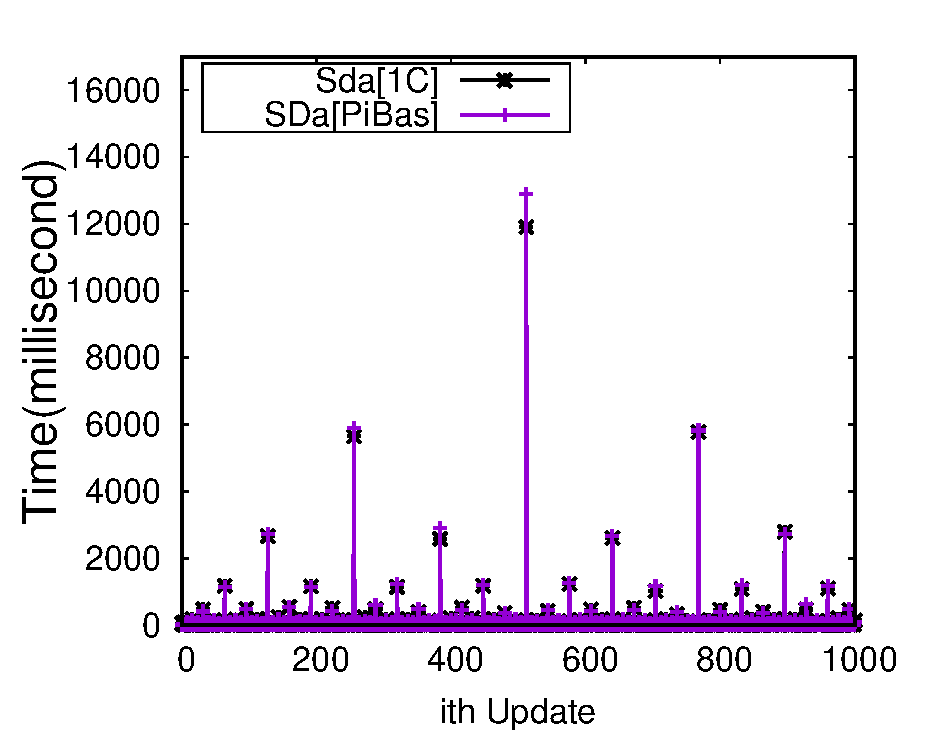
\includegraphics[width=\textwidth]{chapters/iodse/figures/Insert-SDA2.eps}
		\vspace{-0.6cm}
		\caption{}
	\end{subfigure}
 \begin{subfigure}[t]{0.48\linewidth}
		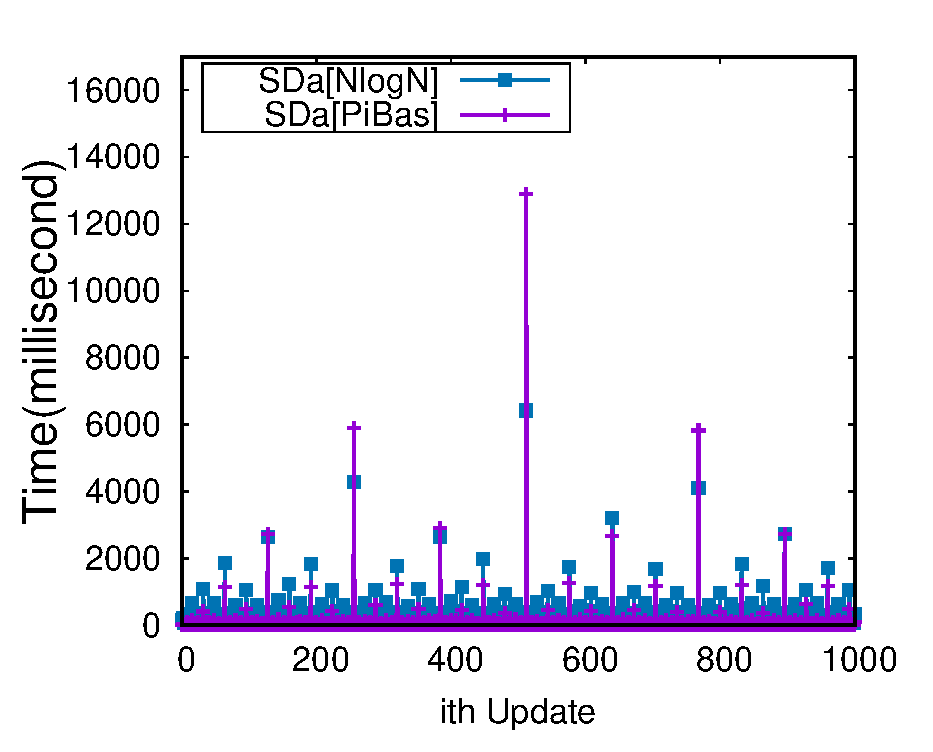
\includegraphics[width=\textwidth]{chapters/iodse/figures/Insert-SDA3.eps}
		\vspace{-0.6cm}
		\caption{}
	\end{subfigure}
	\vspace{-.3cm}
	\caption{Update computation time of amortized schemes for 1K updates starting from an empty dataset (a) \SDa[\OneChoice] vs \SDa[\PiBas] (b) \SDa[\NlogN] vs \SDa[\PiBas] }
	\label{app-fig:update}
% 	\vspace{-.3cm}
\end{figure}

\begin{figure}[t]
	\centering
 \begin{subfigure}[t]{0.48\linewidth}
		\includegraphics[width=\textwidth]{chapters/iodse/figures/UpdateTime.eps}
		\vspace{-0.6cm}
		\caption{}
	\end{subfigure}
 \begin{subfigure}[t]{0.48\linewidth}
		\includegraphics[width=\textwidth]{chapters/iodse/figures/UpdateTime-WAN1.eps}
		\vspace{-0.6cm}
		\caption{}
	\end{subfigure}
	\vspace{-.3cm}	
	\caption{Update computation time for variable database sizes (a) over single machine (b) over WAN machines with 24.7ms network delay and 2.5Gbps bandwidth.}
	\label{fig:wan}
% 	\vspace{-.3cm}
\end{figure}

% \parhead{Amortize Update Cost} Figure~\ref{fig:update}(a) shows \SDa[\NlogN] and \SDa[\PiBas] update time for 1K consecutive updates. In each update, the client fetches and merges some of the previously built levels and then uploads them to the server. Clearly, the update cost depends on the number of previously inserted indexes and increases when more number of indexes need to be merged. We repeated the same experiment for \SDa[\OneChoice] and \SDa[\TwoChoice]. However, since these two schemes show similar behavior to \SDa[\NlogN] and \SDa[\PiBas], we only provide the numbers of the aforementioned scheme which have the minimum and maximum of the update time. As is clear from the figure, as expected, \SDa[\PiBas] has the best update cost for small merges (due to the smallest number of needed entries) and the worst update cost for big merges (due to the random disk accesses). In this experiment, the minimum and maximum observed update time are $2$ms and $15143$ms.

% \begin{figure}
% \centering
% 		\includegraphics[width=0.5\linewidth]{figures/UpdateTime.eps}
% 		%\vspace{-.6cm}
% 		\caption{Update computation time for the de-amortized schemes}
%   \label{fig:updatedeam}
% \end{figure}%

% \begin{figure}[ht]
% 	\centering
% 	\begin{subfigure}[t]{0.48\linewidth}
% 		\includegraphics[width=\textwidth]{figures/UpdateTime.eps}
% 		\vspace{-0.6cm}
% 		\caption{}
% 	\end{subfigure}
%  \begin{subfigure}[t]{0.48\linewidth}
% 		\includegraphics[width=\textwidth]{figures/UpdateTime-WAN1.eps}
% 		\vspace{-0.6cm}
% 		\caption{}
% 	\end{subfigure}
% 	\vspace{-.3cm}
% 	\caption{Update computation time for the de-amortized schemes (a) on a single machine (b) on separate client/server machines with 24.7ms network delay and 2.5Gbps bandwidth.}
% 	\label{fig:updatedeam}
% % 	\vspace{-.3cm}
% \end{figure}
	

\smallskip\noindent\textbf{Update Cost of De-Amortized schemes.} To measure the update performance of our de-amortized schemes, first we measured the update computation time for variable database sizes in memory. According to our experiment (Figure~\ref{fig:wan} (a)), \LSDd[\OneChoice] outperforms other schemes for database sizes above $100K$ which is compatible with its better asymptotics (e.g., \LSDd[\OneChoice] is up to {$2.5\times$} faster than \SDd[\PiBas]\ for database size of 5M). Furthermore, \LSDd[\NlogN] has the worst performance in the memory setting due to the large number of layers it needs to create for each level of the de-amortized framework. \neww{We also provided \LSDd[\PiBas] update time to show our framework is applicable to \SDd[\PiBas] and can reduce its cost from $O(\log^3 N)$ to $O(\log^2 N)$.}
Finally, we re-executed this using HDD storage. We observe that \LSDd[\OneChoice] is still the most efficient scheme in all database sizes. On the other hand, \LSDd[\NlogN] becomes better than \SDd[\PiBas] in bigger database sizes due to its better locality (e.g., \LSDd[\OneChoice] and \LSDd[\NlogN] are {$123\times$ and $5\times$} faster than \SDd[\PiBas]\ for size 5M).


\smallskip\noindent\textbf{Update Over WAN.}
\neww{We measured end-to-end update times when client and server are located on different AWS machines, as above (Figure~\ref{fig:wan} (b)). The performance of memory-based \SDd[\PiBas] worsens due to the round trips for OMAP access and the amount of data that must be transferred over the network (\LSDd[\OneChoice] is {$8-11.3\times$} and \LSDd[\NlogN] is {$1.2-2\times$} faster than \SDd[\PiBas]). That said, the performance of disk-based schemes is similar to the single-machine case as the disk overhead is the dominant cost and the bandwidth is high enough to ``cover'' for the network overhead.}

% \begin{figure*}[ht]
% 	\centering
% 	\begin{subfigure}[t]{0.24\linewidth}
% 		\includegraphics[width=\textwidth]{figures/Search-Comp-DBSize10M-ResultSizeVar-32B-NoCache.eps}
% 		\vspace{-0.8cm}
% 		\caption{}
% 	\end{subfigure}
% 	\begin{subfigure}[t]{0.24\linewidth}
% 		\includegraphics[width=\textwidth]{figures/Search-10pCache.eps}
% 		\vspace{-.8cm}
% 		\caption{}
% 	\end{subfigure}%
% 		\begin{subfigure}[t]{0.24\linewidth}
% 		\includegraphics[width=\textwidth]{figures/Search-20pCache.eps}
% 		\vspace{-.8cm}
% 		\caption{}
% 	\end{subfigure}~
%  	\begin{subfigure}[t]{0.24\linewidth}
% 		\includegraphics[width=\textwidth]{figures/Search-50pCache.eps}
% 		\vspace{-.8cm}
% 		\caption{}
% 	\end{subfigure}~\\
% 	\vspace{-.4cm}
% 	\caption{Search computation time for $|{DB}|=2^{23}$ and variable result size for $|block|=32$B in HDD, (a) 0\% Caching, (b) 10\% Caching, (c) 20\% Caching, (c) 50\% Caching.}
% 	\label{fig:search-var-block}
% 	\vspace{-.2cm}
% \end{figure*}
% we simulated the worst-case number of IO operations they need for each update and compared them in Figure~\ref{fig:update}(b). In this Figure, we provide two simulations. First we assume that the main memory can keep constant number of entries (e.g., $M=2$ entries). In this case, all operations in all schemes would need an IO access because they cannot be kept in the main memory. Therefore, as the figure shows, \SDd[\OneChoice] will be more affected than \SDd[\PiBas] by this  because it needs to do some extra operations like sorting to provide better locality. On the other hand, \SDd[\OneChoice]s would need less number of IO operations than \SDd[\PiBas] and \SDd[\OneChoice] because it does not need OMAP and most of the update cost comes from the OMAP accesses ($\bO(\log^2N)$).

% In the second simulation, we assume that the main memory can keep $\bO(\gamma)$ number of entries. Note that this assumption mostly helps our schemes because the cost of \SDd[\PiBas] does not depends on the available main memory (even in the OMAP part it does not improve the performance). As the figure shows, this amount of memory improve the performance of \SDd[\OneChoice]s because it can execute the sort algorithm more efficiently and does not need to swap-in/out into the hard disk. Therefore, this assumption leads to more than three orders of magnitude less IO in comparison to \SDd[\PiBas]. E.g., in a dataset with size $10^7$, \SDd[\PiBas] needs 150K IOs while \SDd[\OneChoice]s only needs 144 IOs.




\vspace{-10pt}
\section{Conclusion }\vspace{-10pt}
\new{
% While forward-privacy and I/O-efficiency have been described as two 
% \emph{irreconcilable} notions in prior literature,  I
In this work,  
we proposed the first I/O efficient DSE schemes with forward/backward privacy  
by re-visiting prior ``static-to-dynamic" compilers.
% compilers presented by Demertzis et al. \cite{SDa},
% namely the \SDa\ and \SDd\ schemes. 
% These schemes originally were instantiated 
% only with \PiBas, a static SE scheme that offers worst-case I/O efficiency.  
% We observed that \SDa\ can be instantiated with any I/O-efficient static SE scheme to achieve an 
% I/O-efficient DSE scheme that also ensures forward/backward privacy. 
% The only drawback of \SDa\ is that it offers amortized update cost. 
% To overcome this problem, the natural approach was to use the \SDd\ scheme, 
% that de-amortizes the update cost, although we had to incorporate new techniques 
% to it to get it work with the I/O-efficient schemes efficiently. 
First, we came up with a new \emph{oblivious merge} framework, that enabled us to 
place entries for the same keyword close to each other (preserving locality).
Moreover, we optimized performance by replacing oblivious data structures 
% utilized in the original \SDd\cite{SDa} approach. Instead, we opted 
for more lightweight and easier-to-implement oblivious sorting algorithms and linear scans. 
% We named this modified \emph{locality-aware} scheme \LSDd\ as it is influenced from \SDd. 
We implemented both amortized and de-amortized 
% \SDa[$\cdot$] and \LSDd[$\cdot$]\ 
transformations with I/O-efficient static
schemes, such as \OneChoice, \TwoChoice, \NlogN, and \sN~(for s = 3 and 6), and compared 
their search and update times with prior works, overall showcasing our schemes' superior performance in various settings and configurations.
% the original \PiBas\ specific 
% \SDa\ and \SDd\ of \cite{SDa}. 
% Our experiments were performed for variable result size, variable database size and variable block size. 
% We conclude that the I/O-efficient schemes always 
% performed better than the non I/O-efficient ones (both for HDDs and SSDs).
}


%\tgreen{conclusion is vague}
%In this paper, we proposed two families of I/O efficient DSE schemes with 
%forward/backward privacy. The first proposes a static-to-dynamic transformation with amortized update %cost. The second is aiming for schemes with de-amortized update costs proposing a new strategy based on %oblivious sorting. We show that our proposed constructions improve state-of-the art both experimentally %and asymptotically. 


%\chapter{Conclusion}

\appendix
%\if 0
\begin{definition}[Plug] plugging of hole to evaluation context $E$\\
\ensuremath{
1.[~][e] = e \\
2.(E e')[e] = (E [e]) e' \\
3.(w E')[e] = w (E'[e]) \\
4.(E \tau)[e] = (E[e])\tau \\
5.(\pair{E}{e})[e] = \pair{E[e]}{e} \\
6.(\pair{w}{E})[e] = \pair{w}{E[e]} \\
7.(\return{\ell }{E} )[e] = \return{\ell }{E[e]} \\
8.(\proji{E})[e] = \proji{E[e]} \\
9.(\inji{\sumtype{\tau_1}{\tau_2}}{E})[e] = \inji{\sumtype{\tau_1}{\tau_2}}{E[e]} \\
10.(\bind{x}{E}{e'})[e] = \bind{x}{E[e]}{e'}\\ 
11.(\casexp{E}{x}{e_1}{e_2}{\sumtype{\tau_1}{\tau_2}})[e] \\= \casexp{E[e]}{x}{e_1}{e_2}{\sumtype{\tau_1}{\tau_2}}\\
14.(\ret{E}{p})[e] = \ret{E[e]}{p}\\
15. (\select{E}{e'})[e] = \select{E[e]}{e'} \\
16. (\select{w}{E})[e] = \select{w}{E[e]}  \\
%17. (\compEnd{\tau}{E}{e'})[e] = \compEnd{\tau}{E[e]}{e'}\\
%18. (\compEnd{\tau}{w}{E})[e] = \compEnd{\tau}{w}{E[e]} \\ 
}
\end{definition}
\fi 
%\begin{lemma}[RunT]
%If $\runnable{\Pi}{\tau}{c}$ then $\forall{e}.$
%\TValGpcw{e}{\tau}
%\end{lemma}

\begin{lemma}[UniqueType]
If~{\TValGpcw{e}{\tau}}~ and~ {\TValGput{e}{\mathring{\tau}}}~then~
$\tau = \tau'$
\end{lemma}
\textbf{Proof.}
Proof by induction on typing derivation of $e$. \\
\textbf{Case VAR.}
Given, 
\begin{align}
{\TValGpcw{x}{\tau}}  \label{vu1} \\
{\TValGput{x}{\mathring{\tau}}} \label{vu1.1} \\
\intertext{inverting \ref{vu1} we get}
\Gamma(x)=\tau  \label{vu2} \\ 
\rafjudge{\Pi}{c}{pc} \label{vu3} \\
\intertext{inverting \ref{vu1.1} we get}
\Gamma(x)=\mathring{\tau}  \label{vu4} \\ 
\rafjudge{Π}{c}{\mathring{pc}} \label{vu5} \\
\intertext{$\Gamma$ in \ref{vu1} and \ref{vu1.1} are same, so from 
\ref{vu2} and \ref{vu4} we get}
\tau = \mathring{\tau}
\end{align}
\textbf{Case UNIT.}Trivial, as $\void$ can only have type 
$\voidtype$. \\
\textbf{Case FAIL.}Trivial, as $\fail{\tau}$ can only have type $\tau$. \\
\textbf{Case DEL.} Trivial, as $\delexp{p}{q}$ can only have type $\aftype{p}{q}$. \\
\textbf{Case LAM.} Given,
\begin{align}
{\TValGpcw{\lamc{x}{τ_1}{\pc'}{e}}{\func{τ_1}{\pc'}{τ_2}}} \label{lu1} \\
{\TValGput{\lamc{x}{τ_1}
{\pc'}{e}}{\func{τ_1}{\pc'}{\mathring{τ_2}}}} \label{lu2} \\
\intertext{inverting \ref{lu1} we get,}
\TVal{Γ,x\ty τ_1;\pc';u}{e}{τ_2} \label{lu3} \\
\rafjudge{Π}{c}{pc} \label{lu4} \\
u= UB(\func{τ_1}{\pc'}{τ_2}) \label{lu5} \\
\rafjudge{Π}{c}{u} \label{lu6} \\
\intertext{inverting \ref{lu2} we get,}
\TVal{Γ,x\ty τ_1;\pc';u'}{e}{\mathring{τ_2}} \label{lu7} \\
\rafjudge{Π}{c}{\mathring{pc}} \label{lu8} \\
u'= UB(\func{τ_1}{\pc'}{\mathring{τ_2}}) \label{lu9} \\ 
\rafjudge{Π}{c}{u'} \label{lu10} \\
\intertext{One thing to notice here, is that $\tau_1$ and $pc'$ is implicitly
defined in the expression $\lamc{x}{τ_1}{\pc'}{e}$, 
so they are same for both \ref{lu1} and \ref{lu2}. 
So it is sufficient to prove that $\tau_2 = \mathring{\tau_2}$. 
From the definition of UB we know that $u$ 
is the upperbound of all the $pc'$s defined in a type, and these $pc'$s 
must be defined in expression $e$. So we can claim that}
u=u' \label{lu11} \\
\intertext{So, \ref{lu7} can be written as}
\TVal{Γ,x\ty τ_1;\pc';u}{e}{\mathring{τ_2}} \label{lu12} \\
\intertext{from IH \ref{lu12} and \ref{lu3} we get}
\tau_2 = \mathring{\tau_2} \label{lu13}
\end{align}
\textbf{Case TLAM.} Similar to case LAM. \\
\textbf{Case APP.} Given,
\begin{align}
{\TValGpcw{e_1~e_2}{τ}} \label{au1} \\
{\TValGput{e_1~e_2}{\mathring{\tau}}} \label{au2} \\
\intertext{inverting \ref{au1} we get}
\TValGpcw{e_1}{\func{τ'}{\pc'}{τ}} \label{au3} \\
\TValGpcw{e_2}{τ'} \label{au4} \\
\stflowjudge*{\pc}{\pc'} \label{au5} \\
\rafjudge{Π}{c}{pc} \label{au6} \\
\intertext{inverting \ref{au2} we get}
\TValGput{e_1}{\func{\mathring{τ'}}{\mathring{\pc}'}{\mathring{τ}}} \label{au7} \\
\TValGput{e_2}{\mathring{τ}'} \label{au8} \\
\stflowjudge*{\mathring{\pc}}{\mathring{\pc}'} \label{au9} \\
\rafjudge{Π}{c}{\mathring{pc}} \label{au6} \\
\intertext{from \ref{au7} we can infer that $e_1$ is a lambda term, and that
implies that $\mathring{\pc}'$ and $\mathring{τ'}$ is a part of the expression
$e_1$. Thus they can not be different from  $pc'$ and $\tau'$ 
in \ref{au3}. Otherwise $e_1$ will
not typecheck. Thus we can write the following}
pc' = \mathring{pc}' \label{au10} \\
\tau' = \mathring{\tau'} \label{au11} \\
\intertext{ so \ref{au7} can be written as }
\TValGput{e_1}{\func{τ'}{\pc'}{\mathring{τ}}} \label{au12} \\
\intertext{from IH \ref{au3} and \ref{au12} we get}
\tau = \mathring{\tau}
\end{align}
\textbf{Case TAPP.} Similar to APP. \\
\textbf{Case PAIR.} Given,
\begin{align}
\TValGpcw{\pair{e_1}{e_2}}{\prodtype{τ_1}{τ_2}} \label{pu1} \\
\TValGput{\pair{e_1}{e_2}}{\prodtype{\mathring{τ_1}}{\mathring{τ_2}}} \label{pu2} \\
\intertext{inverting \ref{pu1} we get} 
\TValGpcw{e_1}{τ_1} \label{pu3} \\
\TValGpcw{e_2}{τ_2} \label{pu4} \\
\rafjudge{\Pi}{c}{pc} \label{pu5} \\
\intertext{inverting \ref{pu2} we get}
\TValGput{e_1}{\mathring{τ_1}} \label{pu6} \\
\TValGput{e_2}{\mathring{τ_2}} \label{pu7} \\  
\rafjudge{\Pi}{c}{\mathring{pc}} \label{pu8} \\
\intertext{from IH,\ref{pu3} and \ref{pu6} we get}
\tau_1 = \mathring{\tau_1} \label{pu9} \\
\intertext{from IH,\ref{pu4} and \ref{pu7} we get}
\tau_2 = \mathring{\tau_2} \label{pu10} \\
\intertext{from \ref{pu9} and \ref{pu10} we, without loss of generality, can say}
\prodtype{τ_1}{τ_2} = \prodtype{\mathring{τ_1}}{\mathring{τ_2}} 
\end{align}
\textbf{Case UNPAIR.} Given,
\begin{align}
{\TValGpcw{\proji{e}}{τ_i}} \label{uu1} \\
{\TValGput{\proji{e}}{\mathring{τ_i}}} \label{uu2} \\
\intertext{inverting \ref{uu1} we get,}
\TValGpcw{e}{\prodtype{τ_1}{τ_2}}  \label{uu3} \\
\rafjudge{Π}{c}{pc} \label{uu4} \\
\intertext{inverting \ref{uu2} we get,}
\TValGput{e}{\prodtype{\mathring{τ_1}}{\mathring{τ_2}}} \label{uu5} \\
\rafjudge{Π}{c}{\mathring{pc}} \label{uu6} \\
\intertext{from IH, \ref{uu3} and \ref{uu5} we get,}
\prodtype{τ_1}{τ_2} = \prodtype{\mathring{τ_1}}{\mathring{τ_2}} \label{uu7} \\
\intertext{without loss of generality we can write,}
\tau_1 = \mathring{\tau_1} \\
\tau_2 = \mathring{\tau_2} \\
\intertext{thus we can say}
\tau_i = \mathring{\tau_i}
\end{align}
\textbf{Case INJ.} Trivial, as the type is annotated in the expression.
\textbf{Case CASE.} Given,
\begin{align}
\TValGpcw{\casexp{e}{x}{e_1}{e_2}{\sumtype{τ_1}{τ_2}}}{τ} \label{cu1} \\
\TValGput{\casexp{e}{x}{e_1}{e_2}{\sumtype{τ_1}{τ_2}}}{\mathring{τ}} \label{cu2} \\
\intertext{inverting \ref{cu1} we get,}
\TValGpcw{e}{\sumtype{τ_1}{τ_2}} \label{cu3} \\
\protjudge*{\pc}{τ} \label{cu4} \\
\rafjudge{Π}{c}{pc} \label{cu5} \\
\TVal{\Pi;Γ,x\ty τ_1;\pc;\worker}{e_1}{τ} \label{cu6} \\
\TVal{\Pi; Γ,x\ty τ_2;\pc;\worker}{e_2}{τ} \label{cu7} \\
\intertext{inverting \ref{cu2} we get, }
\TValGput{e}{\sumtype{\mathring{τ_1}}{\mathring{τ_2}}} \label{cu8} \\
\protjudge*{\mathring{\pc}}{\mathring{τ}} \label{cu9} \\
\rafjudge{Π}{c}{\mathring{pc}} \label{cu10} \\
\TVal{\Pi;Γ,x\ty \mathring{τ_1};\mathring{\pc};\worker}{e_1}{\mathring{τ}} \label{cu11} \\
\TVal{\Pi;Γ,x\ty \mathring{τ_2};\mathring{\pc};\worker}{e_2}{\mathring{τ}} \label{cu12} \\
\intertext{from IH, \ref{cu3} and \ref{cu8}, we get}
\sumtype{τ_1}{τ_2} = \sumtype{\mathring{τ_1}}{\mathring{τ_2}} \label{cu13} \\
\intertext{without loss of generality we can write,}
\tau_1 = \mathring{τ_1} \label{cu14} \\
\tau_2 = \mathring{τ_2} \label{cu15} \\
\intertext{thus using \ref{cu14} and \ref{cu15}, we can 
write \ref{cu11} and \ref{cu12} as }
\TVal{\Pi;Γ,x\ty {τ_1};\mathring{\pc};\worker}{e_1}{\mathring{τ}} \label{cu16} \\
\TVal{\Pi;Γ,x\ty {τ_2};\mathring{\pc};\worker}{e_2}{\mathring{τ}} \label{cu17} \\
\intertext{from IH, \ref{cu6}(or \ref{cu7}) and \ref{cu16} 
(or \ref{cu17}) we get}
\tau = \mathring{\tau}
\end{align}
\textbf{Case UNITM.} Given,
\begin{align}
%\TValGput{\return{ℓ}{e}}{\says{ℓ}{τ}} \label{unu1} \\
%\TValGput{\return{ℓ}{e}}{\says{ℓ}{\mathring{τ}}} \label{unu2} \\
\intertext{inverting \ref{unu1} we get}
\TValGpcw{e}{τ} \label{unu3} \\
\intertext{   ...   }
\intertext{inverting \ref{unu2} we get}
\TValGput{e}{\mathring{τ}} \label{unu4} \\
\intertext{   ....    }
\intertext{from IH, \ref{unu3} and \ref{unu4} we get,}
\tau = \mathring{\tau} 
\end{align}
\textbf{Case UNITL.} Similar to case UNITM.\\
\textbf{Case BINDM.} Given,
\begin{align}
\TValGpcw{\bind{x}{e'}{e}}{τ} \label{bu1} \\
\TValGput{\bind{x}{e'}{e}}{\mathring{τ}} \label{bu2} \\
\intertext{inverting \ref{bu1} we get,}
\TValGpcw{e'}{\says{ℓ  }{τ'}} \label{bu3} \\
\stflowjudge*{\ell \sqcup pc}{\tau} \\
\TVal{Γ,x\ty τ';ℓ  ⊔ j \sqcup pc;\worker}{e}{τ} \label{3.3} \\
\rafjudge{Π}{c}{pc}
\intertext{inverting \ref{bu2} we get,}
\TValGput{e'}{\says{\mathring{ℓ}}{\mathring{τ}'}} \label{bu4} \\
\TVal{Γ,x\ty \mathring{τ}';\mathring{ℓ}⊔ \mathring \sqcup \mathring{pc};c}{e}{\mathring{τ}} \label{bu5} \\
\intertext{...}
\intertext{From \ref{bu4} we know that $e'$ is an eta term, and 
associated $\mathring{\ell}$ are annotated in $e'$ itself, so 
they are same as $\ell$ and $j$ in \ref{bu3}.
Thus \ref{bu4} can be written as }
\TValGput{e'}{\says{ℓ}{\mathring{τ'}}} \label{bu5} \\
\intertext{From IH,\ref{bu3} and \ref{bu5} we get,}
\tau'=\mathring{\tau}'
\intertext{Thus \ref{bu5} can be written as,}
\TVal{Γ,x\ty τ';ℓ⊔ j \sqcup \mathring{pc};c}{e}{\mathring{τ}} \label{6} \\
\intertext{from IH,\ref{3.3}, \ref{6}, we get,}
\tau = \mathring{\tau}
\end{align}
\textbf{Case ASSUME.} Given,
\begin{align}
\TValGpcw{\assume{e}{e'}}{τ} \label{asu1} \\
\TValGput{\assume{e}{e'}}{\mathring{τ}} \label{asu2} \\
\intertext{inverting \ref{asu1} we get,}
\TValGpcw{e}{\aftype{p}{q}} \label{asu3} \\
\TVal{Π,\langle \aftypep{p}{q}\rangle; Γ;\pc;c}{e'}{τ} \label{asu4} \\
\intertext{...}
\intertext{inverting \ref{asu2} we get,}
\TValGput{e}{\aftype{\mathring{p}}{\mathring{q}}} \label{asu5} \\
\TVal{Π,\langle \aftype{\mathring{p}}{\mathring{q}}\rangle; Γ;\mathring{\pc};c}{e'}{\mathring{τ}} \label{asu6} \\
\intertext{...}
\intertext{from IH, \ref{asu3} and \ref{asu5} we can write,}
\aftype{p}{q} = \aftype{\mathring{p}}{\mathring{q}} \label{asu7} \\
\intertext{So we can write \ref{asu6} as }
\TVal{Π,\langle \aftypep{p}{q}\rangle; Γ;\mathring{\pc}}{e'}{\mathring{τ}} \label{asu8}\\
\intertext{from IH, \ref{asu4} and \ref{asu8} we get,}
\tau = \mathring{\tau}
\end{align}
\textbf{Case WHERE.} Similar to case ASSUME. \\
\textbf{Case RUN.} Trivial,as type $\tau$ is annotated in $run$ epression. \\
\textbf{Case RET.} Straightforward using IH. \\
\textbf{Case COMPEND.}\\
\textbf{Case SELECT.}\\
\PM{in macros.tex file change TValGput with pc as 
$\mathring{pc}$ might not be required}

\begin{lemma}[WaitUniqueT]
If~\TValGpcw{E[\expect{\hat{\tau}}]}{\tau}~and~
\TValGput{E[\expect{\hat{\tau}}]}{\tau'}~then~
$\tau=\tau'$.
\end{lemma}
\textbf{Proof.} We prove it by induction over structure of $E$.\\
\textbf{Case E=[ ].} Given,
\begin{align}
\TValGpcw{[~][\expect{\hat{\tau}}]}{\tau} \label{wuh1} \\
\intertext{i.e.}
\TValGpcw{\expect{\hat{\tau}}}{\tau} \label{wuh2} \\
\intertext{and}
\TValGput{[~][\expect{\hat{\tau}}]}{\tau'} \label{wuh3} \\
\intertext{i.e.}
\TValGput{\expect{\hat{\tau}}}{\tau'} \label{wuh4} \\
\intertext{but from WAIT typing rule we know}
\TValP{\Gamma;\hat{\pc};c}{\expect{\hat{\tau}}}{\hat{\tau}} \label{wuh5} \\
\intertext{Thus \ref{wuh2} and \ref{wuh4} typechecks only when}
\tau = \tau' = \hat{\tau}
\end{align}
\textbf{Case E = E e .} Given,
\begin{align}
\TValGpcw{(E e)[\expect{\hat{\tau}}]}{\tau} \label{wuh1} \\
\intertext{i.e.}
\TValGpcw{E[\expect{\hat{\tau}}]e'}{\tau} \label{wuh2} \\
\intertext{and}
\TValGput{(E e)[\expect{\hat{\tau}}]}{\tau'} \label{wuh3} \\
\intertext{i.e.}
\TValGput{E[\expect{\hat{\tau}}]e}{\tau'} \label{wuh4} \\
\intertext{inverting \ref{wuh2} we get}
\TValGpcw{E[\expect{\hat{\tau}}]}{\func{\tau_1}{pc'}{\tau}} \label{wuh5} \\
\TValGpcw{e}{\tau_1} \label{wuh6} \\
\intertext{...}
\intertext{inverting \ref{wuh4} we get}
\TValGput{E[\expect{\hat{\tau}}]}{\func{\mathring{\tau_1}}{\mathring{pc'}}{\tau'}} \label{wuh7} \\
\TValGput{e}{\mathring{\tau_1}} \label{wuh8} \\
\intertext{$\tau_1$ and $\pc'$ are part of syntax so, }
\tau_1 = \mathring{\tau_1} \\
\pc' = \mathring{\pc'} \\
\intertext{so \ref{wuh7} can be written as,}
\TValGput{E[\expect{\hat{\tau}}]}{\func{\tau_1}{pc'}{\tau'}} \label{wuh9} \\
\intertext{From IH, \ref{wuh5}, and \ref{wuh9} we get,}
{\func{\tau_1}{pc'}{\tau}}= {\func{\tau_1}{pc'}{\tau'}}
\intertext{Thus we get,}
\tau = \tau'
\end{align}
\textbf{Case E= $\mathbf{\pair{E}{e}}$}
\PM{Other cases later.}


\begin{lemma}[stackUniqueT]
If~\TValGpcS{s[\hat{\tau}]}{\tau}~and \TValGpcS{s[\hat{\tau}]}{\tau'}~ then~
$\tau=\tau'$. 
\end{lemma}
\textbf{Proof.} The proof is by induction over typing derivation of $s$.\\
\textbf{Case $\mathbf{s=\emptystack[\tau]}$.}  Given,
\begin{align}
\TValGpcS{\emptystack[\hat{\tau}]}{\tau} \label{stuq1} \\
\TValGpcS{\emptystack[\hat{\tau}]}{\tau'} \label{stuq2}\\
\intertext{but from EMPTY typing rule we know,}
\TValGpcS{\emptystack[\hat{\tau}]}{\hat{\tau}} \\
\intertext{so \ref{stuq1} and \ref{stuq2} typechecks only when}
\tau=\tau'=\hat{\tau}
\end{align}
\textbf{Case $\mathbf{s = \distS{E[\expect{\hat{\tau}}]}{c}{s[\hat{\tau}]}}$.} 
Given,
\begin{align}
\TValGpcS{\distS{E[\expect{\hat{\tau}}]}{c}{s[\hat{\tau}]}}{\tau} \label{stuq3} \\
\TValGpcS{\distS{E[\expect{\hat{\tau}}]}{c}{s[\hat{\tau}]}}{\tau'} \label{stuq4} \\
\intertext{inverting \ref{stuq3} we get,}
\TValGpcw{E[\expect{\hat{\tau}}]}{\tau''} \label{stuq5} \\
\TValGpcS{s[\tau'']}{\tau} \label{stuq6} \\
\stflowjudge*{\pc}{\pc'} \\
\rafjudge{Π}{c}{pc} \\
\intertext{inverting \ref{stuq4} we get}
\TValGpcw{E[\expect{\hat{\tau}}]}{{\tau_1}''} \label{stuq7} \\
\TValGpcS{s[{\tau_1}'']}{\tau'} \label{stuq8} \\
\intertext{from \ref{stuq5} and \ref{stuq7} and lemma WaitUniqueT,}
\tau'' = {\tau_1}'' \\
\intertext{Thus \ref{stuq8} can be written as}
\TValGpcS{s[\tau'']}{\tau'} \label{stuq9} \\
\intertext{from IH, \ref{stuq6} and \ref{stuq9} we get}
\tau = \tau'
\end{align}
\PM{NOTE:- in WaitUnique and stackUniqueT lemma pc is same for both.}

\begin{lemma}[distUniqueT]
If~\TValGpcS{\distcon{e}{c}{s}}{\tau}~and~ \TValGpcS{\distcon{e}{c}{s}}{\tau'}
~then~ $\tau =\tau'$.
\end{lemma}
\textbf{Proof.}
Straightforward proof using lemmas UniqueType and
WaitUniqueT.

\begin{lemma}[$\Gamma$-Weakening]
If \TValGpcw{e}{\tau} and for 
all $\tau'$ and $x \notin dom(\Gamma)$,
\TValP{\Gamma,x\ty\tau';pc;c}{e}{\tau}
\end{lemma}
\textbf{Proof.} 
By Induction on structure of $e$.


\begin{lemma}[CTX]
\PM{subject reduction uses CTX lemma, and CTX lemma needs uniquetypes ?}
If \TValGpcw{E[e]}{\tau} and 
$x\notin dom(\Gamma)$ then
$\exists \tau'$, such that 
\TValP{\Gamma,x\ty\tau',\pc;c}{E[x]}{\tau} and \TValGpcw{e}{\tau'}.
\end{lemma}
\textbf{Proof.}
By induction on structure of $E$.\\
Given,
\begin{equation}\label{300}
\TValGpcw{E[e]}{\tau}
\end{equation}
and we need to prove 
\begin{align}
\exists{\tau'}.\TValGpcw{e}{\tau'} \label{299} \\
\intertext{and}
\TValP{\Gamma,x\ty\tau',\pc;c}{E[x]}{\tau} \label{298}
\end{align}
\textbf{Case E=[ ].}  
Applying definition Plug in \ref{300} 
(i.e.$[~][e] = e$) we get 
\begin{align}
\TValGpcw{e}{\tau} \label{300.5} \\
\intertext{and $\exists{\tau}$ in \ref{299} we get}
\TValGpcw{e}{\tau} \label{301}\\ 
\intertext{from VAR rule for variable $x$}
\TValP{\Gamma,x\ty\tau,\pc;c}{x}{\tau} \label{302} \\
\intertext{from \ref{302} and definition Plug}
\TValP{\Gamma,x\ty\tau,\pc;c}{[~][x]}{\tau} \label{303} \\
\end{align}
{\ref{301} and \ref{303} together proves \ref{299} and \ref{298}}. \\
\textbf{Case E = E e'} 
Applying definition Plug in \ref{300} ($(E e')[e] = E[e] e'$)
\begin{align}
\TValGpcw{E[e]e'}{\tau} \label{304} \\
\intertext{inverting \ref{304}}
\TValGpcw{E[e]}{\func{\tau_1}{pc'}{\tau}} \label{305} \\
\intertext{and}
\TValGpcw{e'}{\tau_1} \label{306} \\
\intertext{inverting \ref{306} using $\Gamma$-Weakening }
\TValP{\Gamma,x\ty\tau',\pc;c}{e'}{\tau_1} \label{307} \\
\intertext{I.H. on \ref{305} we get (destruct IH with $\tau'$)}
\TValGpcw{e}{\tau'} \label{308} \\
\intertext{and}
\TValP{\Gamma,x\ty\tau',\pc;c}{E[x]}{\func{\tau_1}{pc'}{\tau}} \label{309} \\
\intertext{from \ref{309}, \ref{307} and APP we get}
\TValP{\Gamma,x\ty\tau',\pc;c}{E[x]e'}{\tau} \label{310}
\end{align}
{\ref{308} and \ref{310} together proves \ref{299} and \ref{298}}\\ 
\textbf{Case E=$\pair{E}{e'}$}.
Applying definition Plug in \ref{300} ($(\pair{E}{e'})[e] = \pair{E[e]}{e'}$)
and $\tau = \prodtype{\tau_3}{\tau_4}$
\begin{align}
\TValGpcw{\pair{E[e]}{e'}}{\tau} \label{311} \\
\intertext{inverting \ref{311} }
\TValGpcw{E[e]}{\tau_3} \label{312} \\
\intertext{and}
\TValGpcw{e'}{\tau_4} \label{313} \\
\intertext{inverting \ref{312} \ref{313} using $\Gamma$-Weakening }
\TValP{\Gamma,x\ty\tau',\pc;c}{E[e]}{\tau_3} \label{314} \\
\intertext{and}
\TValP{\Gamma,x\ty\tau',\pc;c}{e'}{\tau_4} \label{315}
\intertext{I.H. on \ref{312} we get(destruct IH with $\tau'$)}
\TValGpcw{e}{\tau'} \label{316} \\
\intertext{and}
\TValP{\Gamma,x\ty\tau',\pc;c}{E[x]}{\tau_3} \label{317} \\
\intertext{from \ref{317}, \ref{315} and PAIR rule we get}
\TValP{\Gamma,x\ty\tau',\pc;c}{\pair{E[x]}{e'}}{\tau} \label{318}
\end{align}
{\ref{316} and \ref{318} together proves \ref{299} and \ref{298}}\\
\textbf{Case E=$\proji{E}$}
applying definition Plug in \ref{300} ($(\proji{E})[e] = \proji{E[e]}$)
and $\exists.\tau'$
\begin{align}                                                     
\TValGpcw{\proji{E[e]}}{\tau_i} \label{320} \\
\intertext{inverting \ref{320} and $\tau = \tau_i, i \in \{3,4\}$}
\TValGpcw{E[e]}{\prodtype{\tau_3}{\tau_4}} \label{321} \\
\intertext{applying $\Gamma$-Weakening in \ref{321}}
\TValP{\Gamma,x\ty\tau',\pc;c}{E[e]}{\prodtype{\tau_3}{\tau_4}} \label{322} \\
\intertext{I.H. in \ref{322} we get}
\TValGpcw{e}{\tau'} \label{323} \\
\intertext{and}
\TValP{\Gamma,x\ty\tau',\pc;c}{E[x]}{\prodtype{\tau_3}{\tau_4}} \label{324} \\
\intertext{from \ref{324}, and UNPAIR rule we get}
\TValP{\Gamma,x\ty\tau',\pc;c}{\proji{E[x]}}{\tau} \label{325}
\end{align}
{\ref{323} and \ref{325} together proves \ref{299} and \ref{298}}\\
\textbf{Case E= $\assume{E}{e'}$} 
\PM{(in all of the cases above
 inversion will also have a c actsfor pc premise that has to be added later.)}


\begin{lemma}[WAIT]
If \TValGpcw{E[e]}{\tau} and \TValGpcw{e}{\tau'} then 
\TValGpcw{E[\expect{\tau'}]}{\tau}.
\end{lemma}
\textbf{proof.} Proof by induction over structure of E. \\
Given,
\begin{align}
\TValGpcw{E[e]}{\tau} \label{expect1} \\
\TValGpcw{e}{\tau'}  \label{expect2} \\
\intertext{need to prove} 
\TValGpcw{E[\expect{\tau'}]}{\tau} \label{expect3}\\
\end{align}
\textbf{Case E =[ ]}.
From \ref{expect1} we get
\begin{align}
\TValGpcw{[~][e]}{\tau} \\
\intertext{i.e.}
\TValGpcw{e}{\tau} \label{expect4} \\
%\intertext{from \ref{expect2}, \ref{expect4} and UniqueType lemma we get}
\intertext{but from \ref{expect2}}
\TValGpcw{e}{\tau'} \label{expect4.5}
\intertext{thus}
\tau = \tau'  \label{expect5} \\
\intertext{from WAIT typing rule we get}
\TValGpcw{\expect{\tau'}}{\tau'}  \label{expect6}  \\
\intertext{but $\tau=\tau'$, so \ref{expect6} can be written as}
\TValGpcw{\expect{\tau'}}{\tau} \label{expect7} \\
\intertext{\ref{expect7} can be written as }
\TValGpcw{[~]\expect{\tau'}}{\tau} 
\end{align}
\textbf{Case E = E e'}.
from \ref{expect1} we get
\begin{align}
\TValGpcw{(E~e')[e]}{\tau} \\
\intertext{i.e.}
\TValGpcw{E[e]e'}{\tau} \label{expect8} \\
\intertext{inverting \ref{expect8} we get}
\TValGpcw{E~[e]}{\func{\tau_1}{pc'}{\tau}} \label{expect9} \\
\TValGpcw{e'}{\tau_1} \label{expect10} \\
\rafjudge{\Pi}{c}{pc} \label{expect10.5} \\
\rflowjudge{\Pi}{pc}{pc'} \label{expect10.6} \\
\intertext{from \ref{expect2}, \ref{expect9} and IH we get}
\TValGpcw{E~[\expect{\tau'}]}{\func{\tau_1}{pc'}{\tau}} \label{expect11} \\
\intertext{from \ref{expect10},\ref{expect11},\ref{wait10.5},\ref{wait10.6} and APP typing rule we get}
\TValGpcw{E[\expect{\tau'}]e'}{\tau} \label{expect12} \\
\intertext{\ref{expect12} can be written as}
\TValGpcw{(E~e')[\expect{\tau'}]}{\tau} 
\end{align}
\PM{Other cases for E later.}


\begin{lemma}[RWAIT]
\TValGpcw{v}{\tau'} and
\TValGpcw{E[\expect{\tau'}]}{\tau} then
\TValGpcw{E[v]}{\tau}.
\end{lemma}
\PM{both expect and rexpect can be generalized with e of type tau' instead of wait term
and to be used in subject reduction for case E-Step.}
\PM{Bracketed subject reduction failed bcz of pc' in select.}
\textbf{proof.} Proof by induction over structure of E. \\
Given,
\begin{align}
\TValGpcw{v}{\tau'}  \label{rexpect1} \\
\TValGpcw{E[\expect{\tau'}]}{\tau} \label{rexpect2} \\
\intertext{need to prove}
\TValGpcw{E[v]}{\tau} \label{rexpect3}\\
\end{align}
\textbf{Case E =[ ]}.
from \ref{rexpect2} we get
\begin{align}
\TValGpcw{[~][\expect{\tau'}]}{\tau} \\
\intertext{i.e.}
\TValGpcw{\expect{\tau'}}{\tau} \label{rexpect4} \\
\intertext{from WAIT rule we get }
\TValGpcw{\expect{\tau'}}{\tau'}  \label{rexpect5} \\
\intertext{but from \ref{rexpect4}, $\TValGpcw{\expect{\tau'}}{\tau}$, thus}
\tau=\tau' \label{rexpect6} \\
\intertext{Thus we can write \ref{rexpect1} as }
\TValGpcw{v}{\tau}  \label{rexpect7} \\
\intertext{from definition Plug, \ref{rexpect7} can be written as}
\TValGpcw{[~]v}{\tau} 
\end{align}
\textbf{Case E =E e'}.
from \ref{rexpect2} we get
\begin{align}
\TValGpcw{(E~e')[\expect{\tau'}]}{\tau} \\
\intertext{i.e.}
\TValGpcw{E[\expect{\tau'}]e'}{\tau} \label{rexpect8} \\
\intertext{inverting \ref{rexpect8} we get}
\TValGpcw{E~[\expect{\tau'}]}{\func{\tau_1}{pc'}{\tau}} \label{rexpect9} \\
\TValGpcw{e'}{\tau_1} \label{rexpect10} \\
\rafjudge{\Pi}{c}{pc} \label{rexpect10.5} \\
\rflowjudge{\Pi}{pc}{pc'} \label{rexpect10.6} \\
\intertext{from \ref{rexpect1}, \ref{rexpect9} and IH we get}
\TValGpcw{E~[v]}{\func{\tau_1}{pc'}{\tau}} \label{rexpect11} \\
\intertext{from \ref{rexpect10}, \ref{rexpect11}, \ref{rwait10.5}, \ref{rwait10.6} and APP typing rule we get}
\TValGpcw{E[v]e'}{\tau} \label{rexpect12} \\
\intertext{\ref{rexpect12} can be written as}
\TValGpcw{(E~e')[v]}{\tau}
\end{align}
\PM{Other cases for E later.}
\PM{runnable gives me info about pcs but not  
if e will be typechecked as well, so used UB}



\begin{lemma}[Values are typable at any host and any \pc]
Let $\TValGpcw{v}{\tau}$. If  
$\rafjudge{\Pi}{c'}{pc'}$ and $\rafjudge{\Pi}{c'}{UB(\tau)}$ 
then $\TValGpcdashpc{v}{\tau}$.
\end{lemma}
\textbf{Proof.} Given that,
\begin{align}
\rafjudge{\Pi}{c'}{pc'}   \label{VTH} \\
\rafjudge{\Pi}{c'}{UB(\tau)}  \label{VTH.5} 
\end{align}
Using induction over values.\\ \\
%\textbf{case FAIL.} Using [FAIL] and (\ref{VTH}) we have 
%{\TValGpcdashpc{\fail{\says{\ell}{\tau}}}{\says{\ell}{\tau}}}\\ \\
\textbf{Case UNITM.} Using [UNIT] and (\ref{VTH}) we have  
{\TValGpcdashpc{\void}{\voidtype}}\\ \\
\textbf{Case DEL.} Using [DEL] and (\ref{VTH}) we have 
{\TValGpcdashpc{\delexp{p}{q}}{\aftype{p}{q}}}\\ \\
\textbf{Case PAIR.} Given 
\begin{equation}\label{pairVTH}
{\TValGpcw{\pair{v_1}{v_2}}{\prodtype{τ_1}{τ_2}}}
\end{equation}
Inverting (\ref{pairVTH}) we get 
\begin{equation}\label{pairVTH1}
\TValGpcw{v_1}{τ_1}
\end{equation} 
and
\begin{equation}\label{pairVTH2}
\TValGpcw{v_2}{τ_2}
\end{equation}
By applying induction hypothesis on (\ref{pairVTH1}) and (\ref{pairVTH2}), we get
\begin{equation}\label{pairVTH3}
\TValGpcdashpc{v_1}{τ_1}
\end{equation}
and
\begin{equation}\label{pairVTH4}
\TValGpcdashpc{v_2}{τ_2}
\end{equation}
From rule [PAIR], (\ref{pairVTH3}), (\ref{pairVTH4}), and (\ref{VTH}) we get
{\TValGpcdashpc{\pair{v_1}{v_2}}{\prodtype{τ_1}{τ_2}}}\\ \\
\textbf{Case INJ.} Similar to \textbf{case PAIR}.\\ \\
\textbf{Case UNITL.} Given 
\begin{equation}\label{sealVTH}
{\TValGpcw{\returnv{ℓ }{v}}{\says{ℓ }{τ}}}
\end{equation}
Inverting (\ref{sealVTH}) we get
\begin{equation}\label{sealVTH1}
 \TValGpcw{v}{\tau} 
\end{equation}
By applying induction hypothesis on (\ref{sealVTH1}) we get
\begin{equation}\label{sealVTH2} 
\TValGpcdashpc{v}{τ}
\end{equation}
Thus from rule [SEAL], (\ref{VTH}) and (\ref{sealVTH2}) we get 
{\TValGpcdashpc{\returnv{ℓ  }{v}}{\says{ℓ  }{τ}}}\\ \\
\textbf{Case WHERE.} Given
\begin{equation}\label{whereVTH}
{\TValGpcw{(\where{v_1}{v_2})}{τ}}{}
\end{equation}
Inverting (\ref{whereVTH}) we get
\begin{equation}\label{whereVTH1}
 \TValGpcw{v_2}{\aftype{p}{q}}
\end{equation}
\begin{equation}\label{whereVTH2}
\rafjudge{Π}{\pcmost}{\voice{q}}
\end{equation}
\begin{equation}\label{whereVTH3}
\rafjudge{Π}{\voice{\confid{p}}}{\voice{\confid{q}}}
\end{equation}
\begin{equation}\label{whereVTH4}
\TVal{Π,\langle \aftypep{p}{q}\rangle;Γ;\pc}{v_1}{τ}
\end{equation}
By applying induction hypothesis on (\ref{whereVTH1}) and
and (\ref{whereVTH4}) and $\Pi$-extension rule on 
(\ref{whereVTH4}) we get
\begin{equation}\label{whereVTH5}
 \TValGpcdashpc{v_2}{\aftype{p}{q}}
\end{equation}
\begin{equation}\label{whereVTH6}
\TVal{Π,\langle \aftypep{p}{q}\rangle;Γ;\pc';c'}{v_1}{τ}
\end{equation}
Thus from rule [WHERE], (\ref{VTH}), (\ref{whereVTH2}),  (\ref{whereVTH3}),
 (\ref{whereVTH5}) and (\ref{whereVTH6}) we get
{\TValGpcdashpc{(\where{v_1}{v_2})}{τ}}{} \\ \\
\textbf{Case LAM.} We have 
\begin{equation}\label{lamVTH}
{\TValGpcw{\lamc{x}{τ_1}{\pc''}{e}}{\func{τ_1}{\pc''}{τ_2}}}
\end{equation}
Inverting (\ref{lamVTH}) we get
\begin{align}
\TVal{\Pi;Γ,x\ty τ_1;\pc'';u}{e}{τ_2}  \label{lamVTH1} \\
u = UB(\func{τ_1}{\pc''}{τ_2}) \label{lamVTH1.1} \\
\rafjudge{\Pi}{c}{pc}  \\ 
\rafjudge{\Pi}{c}{u}  \\
\intertext{given in lemma statement} 
\rafjudge{\Pi}{c'}{pc'}  \label{lamvth1.2} \\                                  
\rafjudge{\Pi}{c'}{u}  \label{lamvth1.3} \\ 
\intertext{from \ref{lamvth1.2}, \ref{lamvth1.3}, 
\ref{lamVTH1} and LAM rule we get}
{\TValGpcdashpc{\lamc{x}{τ_1}{\pc''}{e}}{\func{τ_1}{\pc''}{τ_2}}} \\ \\
\end{align}
\textbf{Case TLAM.} Similar to \textbf{case LAM}.\\ \\
%\textbf{Case FAIL.} We have 
%\begin{equation}\label{failVTH}
%\TValGpcw{\fail{\tau}}{\tau}
%\end{equation} 
%From (\ref{VTH}) and [FAIL] rule we have \TValGpcdashpc{\fail{\tau}}{\tau}  
\textbf{Case BRACKET.}
Given,
\begin{align}
{\TValGpcw{\bracket{w_1}{w_2}}{\tau}}  \label{br1} \\
\intertext{inverting \ref{br1} we get}
\protjudge{\delegcontext}{H^\pi}{\tau} \label{br2} \\
\TValGpcw{w_1}{\tau} \label{br3} \\      
\TValGpcw{w_2}{\tau} \label{br4} \\
\intertext{IH on \ref{br3} and \ref{br4}}
\TValGpcdashpc{w_1}{\tau} \label{br5} \\
\TValGpcdashpc{w_2}{\tau} \label{br6} \\
\intertext{from \ref{br5},\ref{br6} and \ref{br2} we get}
{\TValGpcdashpc{\bracket{w_1}{w_2}}{\tau}}
\end{align}

\begin{lemma}[$\pc$ reduction]
 Let \TValGpcw{e}{\tau}.
  For all $\pc, \pc'$, such that
  \rflowjudge{\delegcontext}{\pc'}{\pc} and 
  \rafjudge{Π}{c}{pc'} (and 
\rflowjudge{\delegcontext}{\j(\tau)}{pc'}) then
  \TValP{\varcontext;pc';c}{e}{\tau} holds.
\end{lemma}
\textbf{Proof.}
Using induction. 
\PM{Works for run /ret after adding pc' in run. But
breaks for compEnd and select after incorporating j, as 
j might not flow to reduced pc. So to fix it 
$(\rflowjudge{\delegcontext}{\j(\tau)}{pc'})$ is added
in the lemma statement.
works for bracket/bracket-values}

%\begin{lemma}[CTXpc]
%If~ \TValP{\varcontext;pc';c}{e}{\tau} , $\forall{v}.${\TValGpcw{v}{\tau'}} and
%{\TValGpcw{E[v]}{\tau}}, and \rflowjudge{\delegcontext}{\pc}{\pc'} 
%then {\TValGpcw{E[e]}{\tau}}
%\end{lemma}
%\textbf{Proof.}
%First apply pc reduction in \TValP{\varcontext;pc';c}{e}{\tau}
%with $pc$, then
%apply Lemma CTX.
%

\begin{lemma}[$\Pi$ extension]
If {\TValGpc{e}{\tau}} then 
\TVal{\delegcontext\delegconcat \delexp{p}{q};\varcontext;\pc}{e}{\tau} 
for any $p, q \in \L$.
\end{lemma}
\begin{lemma}[Robust assumption]
 If
        $\rafjudge{\Pi}{\pc}{\voice{b}}$, then
        $\rafjudge{\delegcontext\delegconcat \delexp{a}{b}}{\pc}{\voice{b}}$ for any $a, b \in \L$.
\end{lemma}
\begin{lemma}[Robust Protection]
If
        $\protjudge{\delegcontext}{\pc}{\tau}$,
        then
        $\protjudge{\delegcontext\delegconcat \delexp{a}{b}}{\pc}{\tau}$ for any $a, b \in \L$.
\end{lemma}
\begin{lemma}[Variable substitution]
If \TValP{\Gamma,x:\tau';\pc;c}{e}{\tau} and \TValGpcw{w}{τ'}, then \TValGpcw{\subst{e}{x}{w}}{\tau}.
\end{lemma}
%\begin{proof}
trivial
%\end{proof}
\textbf{Proof.}
Proof is by induction on the typing derivation of $e$.
\\
\textbf{Case LAM.}
Given,
\begin{align}
\TValGpcw{w}{τ'} \label{99} \\
{\TValP{\Gamma,x'\ty \tau';\pc;c}{\lamc{x}{τ_1}{\pc'}{e}}{\func{τ_1}{\pc'}{τ_2}}} \label{100} \\
{\TValP{Γ,x'\ty \tau',x\ty τ_1;\pc';c'}{e}{τ_2}} \label{101} \intertext{inverting \ref{100}}\\
\rafjudge{\Pi}{c'}{\pc'} \label{102} \intertext{clearance of \ref{101}} \\
{\TValGpcdashpc{w}{τ'}} \label{103} \intertext{lemma values host pc and \ref{102}} \\
{\TValP{Γ,x\ty τ_1;\pc';c'}{\subst{e}{x'}{w}}{τ_2}} \label{104} \intertext{IH, \ref{101}, \ref{103}}
\TValGpcw{\lamc{x}{τ_1}{\pc'}{\subst{e}{x'}{w}}}{\tau_2} \intertext{from LAM, and \ref{104}}
\end{align}
\textbf{Case RUN.} Same as before.
\begin{lemma}[Type substitution]
 %Let $\tau'$ be well-formed in $\varcontext, X, \varcontext'$.                     If $\TValP{\varcontext, X, \varcontext';\pc}{e}{\tau}$ then $\TValP{\varcontext, \varcontext'[X \mapsto \tau'];\pc}{e[X \mapsto \tau']}{\tau [X \mapsto \tau']}$.
\end{lemma}
\begin{lemma}[Soundness]\label{lemma:sound}
        If  $e \stepsone e'$ then
        $\outproj{e}{k} \stepsto \outproj{e'}{k}$ for $k ∈ \{1,2\}$.
 \end{lemma}
\textbf{Proof}
By induction on the evaluation of $e$.  All bracketed
rules in Figure~\ref{fig:brackets} except 
\ruleref{B-Step} only expand brackets, so
$\outproj{e}{k} = \outproj{e'}{k}$ for $k \in \{1,2\}$. 
For \ruleref{B-Step}, $\outproj{e}{i} \stepsone \outproj{e'}{i}$  
and $\outproj{e}{j} = \outproj{e'}{j}$ .

\begin{lemma}[Subject Reduction(within a host)]
Let  \TValGpcw{e}{τ} \rafjudge{\Pi}{c}{UB(\tau)}.  If $e \stepsone e'$
%\rafjudge{\delegcontext}{c}{\pc}  
then \TValGpcw{e'}{τ}.
\end{lemma}
\textbf{Proof.} \newline
\textbf{Case E-BINDM.} Given $e={\bind{x}{\returnv{ℓ}{w}}{e_1}}$ and 
$e'= \subst{e_1}{x}{w}$ and also
\begin{equation}\label{bind1}
{\TValGpcw{\bind{x}{\returnv{ℓ}{w}}{e_1}}{τ}}
\end{equation}
From the premises of (\ref{bind1}) we have
\begin{align}
  \TValGpcw{\returnv{ℓ}{w}}{\says{\ell}{\tau'}} \label{eq:sbindm0} \\
  \TValGpcw{w}{\tau'} \label{eq:sbindm1} \\
  \TVal{\Pi;\Gamma,x:\tau';\pc \sqcup \ell \sqcup j;c}
    {e_1}{\tau} \label{eq:sbindm2} \\
  \protjudge{\delegcontext}{\pc \sqcup \ell}{\tau} \label{eq:sbindm4} \\
  \rafjudge{\delegcontext}{c}{\pc}
\end{align}
(Since $\rafjudge{\delegcontext}{c}{\pc}$) applying $\pc$ reduction lemma in 
(\ref{eq:sbindm2})(23) we get $\TValP{\Gamma, x:\tau'; \pc}{e_1}{\tau} \label{eq:sbindm2}$.
Invoking variable substitution lemma, we thus have 
${\TValGpcw{\subst{e_1}{x}{w}}{\tau}}$.
\PM{j flowsto J(tau) is not used and as of now
nothing breaks without it.}
\\ \\
\textbf{Case E-RETSTEP}
\begin{equation}\label{retcon}
{\ret{e_1}{c'}} \stepsone {\ret{e_1'}{c'}}
\end{equation}
Given, $e=\ret{e_1}{c'}$ and $e'=\ret{e_1'}{c'}$ and also
\begin{equation}\label{ret1}
{\TValGpcw{\ret{e_1}{c'}}{\tau}}
\end{equation} 
From the premises of (\ref{ret1}) we get
\begin{align}
{\TValGpcw{e_1}{\tau}}  \label{ret1pr1} \\
\rafjudge{\delegcontext}{c}{\pc}  \label{ret1pr2}
\end{align}
and applying induction hypothesis on the premise of (\ref{retcon})
we get 
\begin{equation}\label{ret1IH}
{\TValGpcw{e_1'}{\tau}}
\end{equation}
From (\ref{ret1IH}) and (\ref{ret1pr2}) we have
${\TValGpcw{\ret{e_1'}{c'}}{\tau}}$ \\ \\
\textbf{E-COMPEND} Given,
$e=(\compEnd{\tau}{\returnv{\ell_1}{w}}{\returnv{\ell_2}{w}})$ and  
$e'=\returnv{\ell_1 \wedge \ell_2}{w}{j_1 \sqcup j_2}$
and also, 
\begin{equation}\label{ce1}
\TValGpcw{\compEnd{\tau}{\returnv{\ell_1}{w}}{\returnv{\ell_2}{w}}}
{\says{\ell_1 \wedge \ell_2}{\tau}{j_1 \sqcup j_2}} 
\end{equation}
Inverting (\ref{ce1})
\begin{align}
\TValGpcw{\returnv{\ell_1}{w}}{\says{\ell_1}{τ}} \label{ce2}\\
\TValGpcw{\returnv{\ell_2}{w}}{\says{\ell_2}{τ}} \label{ce3}\\
\confid{c} \rhd \says{\ell_1}{\tau} \label{ce4}\\
\confid{c} \rhd \says{\ell_2}{\tau}  \label{ce5}\\
\rafjudge{\Pi}{c}{pc} \label{ce6}\\
%\stflowjudge*{pc} \label{ce7}\\
%\stflowjudge*{pc}  \label{ce7}\\
\end{align}
Inverting (\ref{ce2}) or (\ref{ce3}) further, we get
\begin{equation}\label{ce8}
\TValGpcw{w}{\tau}
\end{equation}
From rule [UNITL], (\ref{ce8}) and (\ref{ce6}) we can say
$\TValGpcw{\returnv{\ell_1 \wedge \ell_2}{w}{j_1 \sqcup j_2}}
{\says{\ell_1 \wedge \ell_2}{\tau}{j_1 \sqcup j_2}}$ \\ \\
\textbf{Case E-COMPAREFAIL.} Trivial, as $\fail{\tau}$ typechecks
with any protected type, and based on our type-system $\tau$ is always 
a protected type.\\ \\
\textbf{Case E-SELECT.}
Given,
$e = \select{\returnv{\ell_1}{w_1}}{\returnv{\ell_2}{w_2}}{\ell}$ 
and 
$e'= \returnv{\ell}{w_1}$ 
where $\ell = \ell_1 \sqcup \ell_2$ and $j=j_1 \sqcup j_2$.
The following is also given. 
\begin{equation}\label{sel1}
{\TValGpcw{\select{\returnv{\ell_1}{w_1}}{\returnv{\ell_2}{w_2}}{\ell}}{\says{\ell}{τ}}}
\end{equation}
Inverting (\ref{sel1}) we get the following,
\begin{align}
\TValGpcw{\returnv{\ell_1}{w_1}}{\says{\ell_1}{τ}} \label{se2}\\
\TValGpcw{\returnv{\ell_2}{w_2}}{\says{\ell_2}{τ}} \label{se3}\\
\rafjudge{Π}{c}{pc} \label{se4}\\
%\stflowjudge*{\pc} \label{se5} \\
%\stflowjudge*{\pc} \label{se6}
\end{align}
Further inverting (\ref{se2}) we get,
\begin{equation}\label{se7}
\TValGpcw{w_1}{\tau}  
\end{equation} 
Thus from rule [UNITL], (\ref{se7}) and (\ref{se4}) we can argue,
$\TValGpcw{\returnv{\ell}{w_1}}{\says{\ell_1}{τ}}$ \\ \\
\textbf{Case E-SELECTOR.} Similar to above. The only diffrence is we need to
invert both (\ref{se2}) and (\ref{se3}) 
and argue both $\TValGpcw{\returnv{\ell}{w_1}}{\tau}$
and $\TValGpcw{\returnv{\ell}{w_2}}{\tau}$ holds.\\ \\                    
\textbf{Case E-SELECTFAIL.} Trivial, as $\fail{\tau}$ typechecks for any
protected type, and based on our type-system $\tau$ is always
a protected type.\\ \\. \\ \\
\textbf{CasecW-COMPEND1} \PM{not sure if this required or the Pi extension works}
Given 
${\config*{\compEnd{\tau}{(\where{w}{v})}{e}}} \stepsone
{\config*{\where{(\compEnd{\tau}{w}{e})}{v}}}$ where
$e=\compEnd{\tau}{(\where{w}{v})}{e}$ and 
$e'=\where{(\compEnd{\tau}{w}{e})}{v}$ and
\begin{equation}\label{cew}
{\TValGpcw{\compEnd{\tau}{\where{w}{v}}{e}}{\says{(\ell_1 \wedge \ell_2 )}
{\tau}{j_1 \sqcup j_2}}}
\end{equation}
From the premises of (\ref{cew}) we get the following
\begin{align}
\TValGpcw{\where{w}{v}}{\says{\ell_1}{τ}} \label{cew1}\\
\TValGpcw{e}{\says{\ell_2}{τ}} \label{cew2}\\
\confid{c} \rhd \says{\ell_1}{\tau} \label{cew3}\\
\confid{c} \rhd \says{\ell_2}{\tau} \label{cew4}\\
\rafjudge{\Pi}{c}{pc}  \label{cew5} \\
\end{align}
Further inverting (\ref{cew1}) we get
\begin{align}
\TValGpcw{v}{\aftype{p}{q}}\label{cew8} \\
\rafjudge{Π}{\pcmost}{\voice{q}} \label{cew9} \\
\rafjudge{Π}{\voice{\confid{p}}}{\voice{\confid{q}}} \label{cew10}\\
\TVal{Π,\langle \aftypep{p}{q}\rangle;Γ;\pc}{w}
{\says{\ell_1}{τ}} \label{cew11}
\end{align}
We need to prove that 
\begin{equation}\label{cew12}
\TValGpcw{\where{(\compEnd{\tau}{w}{e})}{v}}{\says{(\ell_1 \wedge \ell_2 )}
{\tau}{j_1 \sqcup j_2}}
\end{equation}
From  (\ref{cew3}),(\ref{cew4}),(\ref{cew5}), (\ref{cew6}), (\ref{cew7}),
(\ref{cew11}), and extending delegation context in (\ref{cew2}) we can prove 
\begin{equation}\label{cew13}
\TVal{Π,\langle \aftypep{p}{q}\rangle;Γ;\pc}
{\compEnd{\tau}{w}{e}}{\says{(\ell_1 \wedge \ell_2 )}
{\tau}{j_1 \sqcup j_2}}
\end{equation}
From (\ref{cew8}),(\ref{cew9}),(\ref{cew10}),(\ref{cew13}),  
and [WHERE] rule we can argue (\ref{cew12}) is true. \\ \\
\textbf{Case W-COMPEND2.} Similar to the above case.\\
\textbf{Case W-SELECT1.} Similar to  \textbf{case W-COMPEND1}.\\
\textbf{Case W-SELECT2.} Similar to \textbf{case W-COMPEND1}.\\ \\
\textbf{Case B-SELECT.} Given,
\begin{align}
{\select{\bracket{w_1}{w_2}}{\bracket{w_1'}{w_2'}}{\tau}} 
& \stepsone 
& {\bracket{\select{w_1}{w_1'}{\tau}}{\select{w_2}{w_2'}{\tau}}} \label{bse1} 
\end{align}
\begin{align}
\TValGpcw{{\select{\bracket{w_1}{w_2}}{\bracket{w_1'}{w_2'}}{\tau}}}{\tau} \label{bse2}\\
\intertext{ We need to prove}
\TValGpcw{\bracket{\select{w_1}{w_1'}{\tau}}{\select{w_2}{w_2'}{\tau}}}{\tau}
\intertext{inverting \ref{bse2} we get(here $\ell = {\ell_1 \join \ell_2}
j={j_1 \join j_2}$)}
\TValGpcw{\bracket{w_1}{w_2}}{\says{\ell_1}{τ}} \label{bse3} \\
\TValGpcw{\bracket{w_1'}{w_2'}}{\says{\ell_2}{τ}} \label{bse4} \\
\rafjudge{Π}{c}{pc} \label{bse5} \\
\intertext{inverting \ref{bse3} and \ref{bse4}}
\TValGpcw{w_1}{\says{\ell_1}{τ}} \label{bse8} \\
\TValGpcw{w_2}{\says{\ell_1}{τ}} \label{bse9} \\
\TValGpcw{w_1'}{\says{\ell_2}{τ}} \label{bse10} \\
\TValGpcw{w_2'}{\says{\ell_2}{τ}} \label{bse11} \\
\stflowjudge*{\H^\pi}{\ell_1} \label{bse11.1} \\
\stflowjudge*{\H^\pi}{\ell_2} \label{bse11.2} \\
\intertext{from \ref{bse11.1} and \ref{bse11.2} we get}
\stflowjudge*{\H^\pi}{\ell_1 \join \ell_2} \label{bse11.3} \\
\intertext{applying values pc in \ref{bse8}, \ref{bse9}, \ref{bse10}
\ref{bse11} with pc' as
$pc \join \ell_1 \join \ell_2 $ we get}
\TValGpcc{w_1}{\says{\ell_1}{τ}} \label{bse12} \\ 
\TValGpcc{w_2}{\says{\ell_1}{τ}} \label{bse13} \\ 
\TValGpcc{w_1'}{\says{\ell_2}{τ}} \label{bse14} \\ 
\TValGpcc{w_2'}{\says{\ell_2}{τ}} \label{bse15} \\
\intertext{from \ref{bse12},\ref{bse14},\ref{bse6}, \ref{bse7}, \ref{bse5} 
and SELECT rule we get}
\TValGpcc{\select{w_1}{w_1'}{\tau}}{\tau} \label{bse12} \\
\intertext{from \ref{bse13},\ref{bse15},\ref{bse6}, \ref{bse7}, \ref{bse5} and SELECT 
rule we get}
\TValGpcc{\select{w_2}{w_2'}{\tau}}{\tau} \label{bse13} 
%\intertext{from}
\end{align}
\begin{lemma}[Subject reduction(inter-host)]
If {\TValGpcS{\distcon{e}{c}{s}}{\tau}} and 
$\distcon{e}{c}{s} \Longrightarrow \distcon{e'}{c'}{s'}$ holds, then
{\TValGpcS{\distcon{e'}{c'}{s'}}{\tau}}.
%if $\rafjudge{\Pi}{c'}{pc}$. 
\end{lemma}
\textbf{Proof.}Induction over typing derivation of $e$.\\
\textbf{Case E-RUN}.
Given,
\begin{align}
{\distcon{E[\run{\hat{\tau}}{e}{c'}]}{c}{s}} \Longrightarrow {\distcon{\ret{e}{c}}{c'}{\stackapp{E[\expect{\hat{\tau}}]}{c}{s}}} \\
\TValGpcS{\distcon{E[\run{\hat{\tau}}{e}{c'}]}{c}{s}}{\tau} \label{sr1} \\
%\rafjudge{{\Pi}^{c'}}{c'}{pc}  \label{sr1.1} \\
\intertext{need to prove}
\TValGpcS{\distcon{\ret{e}{c}}{c'}{\stackapp{E[\expect{\hat{\tau}}]}{c}{s}}}{\tau} \label{sr2}
\intertext{Inverting \ref{sr1} we get}
\TValGpart{E[\run{\hat{\tau}}{e}{c'}]}{\tau'}{c'}\label{sr3} \\
\TValGpcS{s[\tau']}{\tau} \label{sr4} \\
\rafjudge{\Pi}{c}{pc} \label{sr5} \\
\stflowjudge*{pc}{pc'} \label{sr6} \\
\intertext{applying lemma CTX to \ref{sr3} we get} 
\TVal{{{\Pi}^{c}};\Gamma;pc';c}{\run{\hat{\tau}}{e}{c'}}{\hat{\tau}}\label{sr7} \\
%\TValP{\Gamma,x\ty \hat{\tau};pc';c}{E[x]}{\tau'[x\notin dom(\Gamma)]} \label{sr8} \\
\intertext{inverting \ref{sr7} we get}
\TVal{{{\Pi}^{c'}};\Gamma,\hat{\pc};c'}{e}{\hat{\tau}} \label{sr9} \\
\rafjudge{{\Pi}^{c}}{c}{pc'} \label{sr9.5} \\
\stflowjudge*{pc'}{\hat{pc}} \label{sr10} \\
\intertext{applying pc-reduction on \ref{sr9} with $\pc$ we get }
\TVal{{\Pi}^{c'};\Gamma,pc;c'}{e}{\hat{\tau}} \label{sr9.6} \\
\intertext{applying clearance in \ref{sr9.6}}
\rafjudge{{\Pi}^{c'}}{c'}{pc}  \label{sr9.7 we get} \\
\intertext{applying clearance lemma in \ref{sr9}}
\rafjudge{{\Pi}^{c'}}{c'}{\hat{pc}} \label{sr11} \\ 
\intertext{from \ref{sr6} and \ref{sr10} we get}
\stflowjudge*{pc}{\hat{pc}} \label{sr12} \\
\intertext{from \ref{sr11} and \ref{sr9} and \ref{sr11} and RET we get}
\TVal{{\Pi}^{c'};\Gamma,\hat{\pc};c'}{\ret{e}{c}}{\hat{\tau}} \label{sr13} \\
\intertext{from \ref{sr3} and \ref{sr7} and WAIT lemma we get}
\TValGpcc{E[\expect{\hat{\tau}}]}{\tau'}\label{sr13.5} \\
\intertext{from \ref{sr4}, \ref{sr5}, \ref{sr6},\ref{sr13.5} and TAIL rule we get}
\TValGpcS{\stackapp{E[\expect{\hat{\tau}}]}{c}{s[\hat{\tau}]}}{\tau} \label{sr14} \\
\intertext{from \ref{sr12},\ref{sr13},\ref{sr14} \ref{sr9.7} and HEAD rule we get}
\TValGpcS{\distcon{\ret{e}{c}}{c'}{\stackapp{E[\expect{\hat{\tau}}]}{c}{s}}}{\tau} \label{sr2}
\end{align}
\textbf{Case E-RETV}. Given, \\
\begin{align}
{\distcon{\ret{w}{c}}{c'}{\stackapp{E[\expect{\tau'}]}{c}{s}}} \Longrightarrow {\distcon{E[w]}{c}{s}} \\
\TValGpcS{\distcon{\ret{w}{c}}{c'}{\stackapp{E[\expect{\tau'}]}{c}{s}}}{\tau} \label{retv1} \\
\rafjudge{\Pi}{c}{pc}  \label{retv1.1} \\
\intertext{need to prove}
\TValGpcS{\distcon{E[w]}{c}{s}}{\tau} \label{retv2} \\
\intertext{inverting \ref{retv1} we get}
\TValP{\Gamma;pc';c'}{\ret{w}{c}}{\tau'} \label{retv3} \\
\TValGpcS{\stackapp{E[\expect{\tau'}]}{c}{s}[\tau']}{\tau} \label{retv4} \\
\stflowjudge*{pc}{pc'} \label{retv5} \\
\rafjudge{\Pi}{c'}{pc} \label{retv6} \\
\intertext{inverting \ref{retv3} we get} 
\TValP{\Gamma;pc';c'}{w}{\tau'} \label{retv7} \\ 
\rafjudge{\Pi}{c}{UB(\tau')} \label{retv7.5} \\
\rafjudge{\Pi}{c'}{pc'} \label{retv8} \\
\intertext{inverting \ref{retv4}}
\TValP{\Gamma;\hat{pc};c}{E[\expect{\tau'}]}{\hat{\tau}} \label{retv9} \\
\stflowjudge*{pc}{\hat{pc}} \label{retv10} \\ 
\rafjudge{\Pi}{c}{pc} \label{retv11} \\
\TValGpcS{s[\hat{\tau}]}{\tau} \label{retv12} \\
\intertext{applying clearance lemma on \ref{retv9}}
\rafjudge{\Pi}{c}{\hat{pc}} \label{retv13} \\
\intertext{from \ref{retv13}, \ref{retv7}, \ref{retv7.5} and ValuesHost lemma}
\TValP{\Gamma;\hat{pc};c}{w}{\tau'} \label{retv14} \\
\intertext{pc reduction in \ref{retv14}}
\TValP{\Gamma;{pc};c}{w}{\tau'} \label{retv14.1} \\
\intertext{clearance lemma on \ref{retv14.1} }
\rafjudge{{\Pi}^{c}}{c}{pc} \label{retv14.2} \\
\intertext{from \ref{retv14}, \ref{retv9} and WAITR lemma }
\TValP{\Gamma;\hat{pc};c}{E[w]}{\hat{\tau}} \label{retv15} \\  
\intertext{from \ref{retv15}, \ref{retv10}, \ref{retv12}, \ref{retv14.2} 
and HEAD rule we get}
\TValGpcS{\distcon{E[w]}{c}{s}}{\tau} 
\end{align}
\textbf{Case E-DSTEP.}\PM{generalize WAIT RWAIT lemma first.}
\PM{check if UB() condition is required in run}
\textbf{Case B-DSTEP.}
\textbf{Case B-RET.} Given,
\begin{align}
{\TValGpcw{\ret{\bracket{e_1}{e_2}}{c'}}{\says{c{^a}}{\tau}{\jmath({\tau})}}} \label{bret0} \\
\ret{\bracket{e_1}{e_2}}{c'} \stepsone \bracket{\ret{e_1}{c'}}{\ret{e_2}{c'}} 
\label{bret1} \\
\intertext{inverting \ref{bret0} we get,} 
\TValGpcw{\bracket{e_1}{e_2}}{\tau} \label{bret2} \\
\rafjudge{\Pi}{c'}{UB(\tau)} \label{bret2.2} \\
\rafjudge{\Pi}{c}{pc} \label{bret2.3} \\
\intertext{inverting \ref{bret2} we get,}
\TValGpcc{e_1}{\tau} \label{bret3} \\
\TValGpcc{e_2}{\tau} \label{bret4} \\
\stflowjudge*{H^{\pi}}{\tau} \label{bret5} \\
\rafjudge{\Pi}{c}{pc} \label{bret6} \\
\stflowjudge*{H^{pi} \join pc}{pc'} \label{bret7} \\
e_1 = v_1  \iff e_2 \ne v_2 \label{bret8} \\
\intertext{applying clearance lemma in \ref{bret3} we get,}
\rafjudge{\Pi}{c}{pc'} \label{bret9} \\
\intertext{from \ref{bret3}, \ref{bret9}, \ref{bret2.2} and RET rule we get}
\TValGpcc{\ret{e_1}{c'}}{\says{c^a}{\tau}{\jmath{(\tau)}}} \label{bret10} \\
\intertext{Similarly, from \ref{bret4}, \ref{bret9}, \ref{bret2.2} and RET rule we get,}
\ret{e_2}{c'}{\says{c^a}{\tau}{\jmath{(\tau)}}} \label{bret11} \\
\intertext{from \ref{bret8} we can say the following(\PM{or argue that 
any ret expression is not a value}),}
\ret{e_1}{c'} = v_1  \iff \ret{e_2}{c'} \ne v_2 \label{bret12}  \\
\intertext{from \ref{bret10},\ref{bret11},
\ref{bret12},\ref{bret2.3},\ref{bret5},\ref{bret7} and BRACKET rule we get,}
\TValGpcw{\bracket{\ret{e_1}{c'}}{\ret{e_2}{c'}}}{\says{c^a}{\tau}{\jmath{(\tau)}}}
\end{align}
%\textbf{Case B-RETV.}






\textbf{Example where propagation fails in RUN/RET.}\\
$\config*{\run{\tau}{(\assume{e_1}{e_2})}{c'}} \stepsone 
\configh*{\ret{(\assume{e_1}{e_2})}{c}} \stepsone^{*}
\configh*{\ret{(\assume{v}{e_2})}{c}} \stepsone
\configh*{\ret{(\where{e_2}{v})}{c}} \stepsone^{*}
\configh*{\ret{(\where{w}{v})}{c}}
$ \newline
Now we can step to \\
$\configh*{\where{(\ret{w}{c})}{v}}$ OR \\
$\config*{\where{w}{v}}$.\\ \\
First one propagates $\where{}{}$ term
and gets stuck as we dont have an evaluation rule for that
and the second one uses [E-RETV] rule 
and does not propagate the $\where{}{}$ term.

\section{Examples.}
In example 1, c runs the code that has authority as same as $a \vee b$
but needs a value that has integrity and confidentiality of $a \wedge b$.

\begin{figure*}
\begin{flushleft}
  \rulefiguresize
\begin{mathpar}
\func{\tau}{a \vee b}{\says{(a \wedge b)}{\tau}} \\
\lamc{x}{\tau}{a \vee b}\\
{\compEnd{\says{(a \wedge b)}{\tau}}{(\run{\says{a}{\tau}}{(\bind{y}{x}
{\returnv{a}{x}})}{a})}{(\run{\says{b}{\tau}}{(\bind{y}{x}
{\returnv{b}{x}})}{b})}}
\hfill
\end{mathpar}
\end{flushleft}
\caption{example 1}
\label{fig:example 1}
\end{figure*}

%\section{Flow limited authorization for quorum replication}
\label{sec:fullrules}
\label{appendix}
\label{sec:ubrules}
\if 0
\begin{figure}[h]
  \small
  \[
    \begin{array}{rcl}
      \multicolumn{3}{l}{ \Pi \in {\{"c","i","a"\}}  \text{  (projections)}} \\
      \multicolumn{3}{l}{ n \in \N \text{  (primitive principals)}} \\
      \multicolumn{3}{l}{ x \in \mathcal{V} \text{  (variable names)}} \\
      \\
      p,\ell,\pc &::=&  n \sep \top \sep \bot \sep p^{\Pi} \sep p \wedge p\sep p \vee p \\[0.4em]
                   &\sep & p \sqcup p \sep p \sqcap p \sep \selor{p}{p} \sep \comor{p}{p} \\[0.4em]
      \tau &::=& \voidtype \sep X \sep \sumtype{\tau}{\tau} \sep \prodtype{\tau}{\tau} \\[0.4em]
         & \sep & \func{\tau}{\pc}{\tau} \sep \tfunc{X}{\pc}{\tau} \sep \says{\ell}{\tau}  \\[0.4em]
      v &::=& \void \sep \returnv{\ell}{v} \sep \injia{\sumtype{\tau}{\tau}}{v} \sep \paira{v}{v}{\tau} \\[0.4em]
        & \sep & \lamc{x}{\tau}{\pc}{e} \sep \tlam{X}{\pc}{e}  \\[0.8em]
      f &::=& v \sep  \faila{\tau} \\[0.8em]
      e &::=& f \sep x \sep e~e \sep e~\tau \sep \return{\ell}{e} \sep 
             \paira{e}{e}{\tau} \\[0.4em]
        & \sep & \proji{e} \sep \injia{\sumtype{\tau}{\tau}}{e} \sep \bind{x}{e}{e}\\[0.4em]
        & \sep & \casexpan{e}{x}{e}{e}{\tau} \\[0.4em]
        & \sep & \runa{\tau}{e}{p}  \sep \ret{e}{p}\\[0.4em]
        & \sep & \selecta{e}{e}{\tau} \sep \comparea{\tau}{e}{e} \sep \expecta{\tau}
    \end{array}
  \]
  \caption{Type annotated FLAQR Syntax (Full version).}
  \label{fig:Annotatedsyntax}
\end{figure}
\fi

\vspace{-1em}
\begin{figure}[h]
{\small
\begin{flalign*}
   \UB{\func{\tau_1}{pc}{\tau_2}} &= \UB{\tau_1} \join pc \join \UB{\tau_2} \\
   \UB{\tfunc{X}{pc}{\tau}} &= pc \join \UB{\tau} \\
   \UB{\says{\ell}{\tau}} &= \UB{\tau} \\
   \UB{\sumtype{\tau_1}{\tau_2}} &= \UB{\tau_1} \join \UB{\tau_2} \\
   \UB{\prodtype{\tau_1}{\tau_2}} &= \UB{\tau_1} \join \UB{\tau_2} \\
   \UB{\voidtype} &= \bot
\end{flalign*}
}
\vspace{-1em}
\caption{Clearance function}
\label{fig:UBFunction}
\end{figure}
\vspace{-1em}
\begin{figure}[h]
 {\small
  \begin{mathpar}
\erule{E-AppFailL}{}{{\lamc{x}{\tau}{pc}{\faila{\func{\tau}{pc}{\tau'}}}}~e}{\faila{\tau'}}\\

\erule{E-TAppFail}{}{\faila{\tfunc{X}{pc}{\tau}}~\tau'}{{\faila{\subst{\tau}{X}{\tau'}}}}


\erule{E-CaseFail}{}{\casexpan{\faila{\tau'}}{x}{e_1}{e_2}{}
{}}{\faila{\tau}}

\erule{E-PairFailL}{}{\paira{\faila{\tau_1}}{f_2}{\prodtype{\tau_1}{\tau_2}}}{\faila{\prodtype{\tau_1}{\tau_2}}}

\erule{E-PairFailR}{}{\paira{f_1}{\faila{\tau_2}}{\prodtype{\tau_1}{\tau_2}}}{\faila{\prodtype{\tau_1}{\tau_2}}} \hfill
\end{mathpar}
}
\vspace{-1em}
\caption{ Remaining cases for propagation of $\fail{}$ terms. }
\label{fig:Fullfailprop}
\end{figure}
\vspace{-1em}
\begin{figure}[h]
{\small
\begin{align*}
\mathscr{C}(\voidtype)                                       &=  \voidtype \\
\mathscr{C}(\sumtype{\tau_1}{\tau_2})                        &=  \sumtype{\mathscr{C}(\tau_1)}{\mathscr{C}(\tau_2)}\\
\mathscr{C}(\prodtype{\tau_1}{\tau_2})                       &=  \prodtype{\mathscr{C}(\tau_1)}{\mathscr{C}(\tau_2)}\\
\mathscr{C}(\func{\tau_1}{pc}{\tau_2})                       &=  \func{\mathscr{C}({\tau_1})}{pc}{\mathscr{C}({\tau_2})}\\
\mathscr{C}(\tlam{X}{pc}{\tau})                              &= \tlam{X}{pc}{\mathscr{C}(\tau)}\\
\mathscr{C}(\says{(\selor{\ell_1}{\ell_2})}{\tau})           &=  \says{(\ell_1 \vee \ell_2)}{\mathscr{C}{(\tau)}}\\
\mathscr{C}(\says{(\comor{\ell_1}{\ell_2})}{\mathscr{\tau}}) &=  \says{(\ell_1 \wedge \ell_2)}{\mathscr{C}{(\tau)}}\\
 \textsf{(otherwise)~} \mathscr{C}(\says{\ell}{\tau})                               &=  \says{\ell}{\mathscr{C}(\tau)} 
\end{align*}
}
\label{fig:Cfunction}
\vspace{-1em}
\caption{$\mathscr{C}$ function on types.}
\end{figure}

\begin{figure}
{\small
%\begin{flalign*}
%& \boxed{\readjudge{\Pi}{p}{\tau}} &
%\end{flalign*}
\begin{mathpar}
\Rule{R-Unit}
     {}
     {\readjudge{\Pi}{p}{\void}}
\Rule{R-TFun}
           {
            \readjudge{\Pi}{p}{\tau}
           }
           {\readjudge{\Pi}{p}{\tfunc{X}{pc}{\tau}}}

\Rule{R-Sum}
     {\readjudge{\Pi}{p}{\tau_1} \\\\
      \readjudge{\Pi}{p}{\tau_2}
     }
     {\readjudge{\Pi}{p}{\sumtype{\tau_1}{\tau_2}}}

\Rule{R-Prod}
     {\readjudge{\Pi}{p}{\tau_1} \\\\
      \readjudge{\Pi}{p}{\tau_2}
     }
     {\readjudge{\Pi}{p}{\prodtype{\tau_1}{\tau_2}}}

\Rule{R-Lbl}
        {\rafjudge{\delegcontext}{p^{\confid}}{\ell^{\confid}} \\\\
         \readjudge{\Pi}{p}{\tau} 
        }
        {\readjudge{\delegcontext}{p}{\says{\ell}{\tau}}}

\Rule{R-Fun}
           {
            \readjudge{\delegcontext}{p}{\tau_1} \\\\
            \readjudge{\delegcontext}{p}{\tau_2}
           }
          {\readjudge{\Pi}{p}{\func{\tau_1}{\pc}{\tau_2}}}
\end{mathpar}
}
\caption{Reads judgments.}
\label{fig:readjudgment}
\end{figure}
\begin{figure}
  {\small
\begin{flalign*}
\last(x,y,&\blame,\ell_1,\ell_2) =~ \MATCH~ (x,y)~ \WITH \\
|~& (\returnv{\ell}{v_1},\returnv{\ell}{v_2}) =  \\
&~ \IF~ \entails{\blame}{\inF{\ell_1}{\FN}}~ \THEN~ \blame \\
&~\ELSE~\IF~ \entails{\blame}{\inF{\ell_2}{\FN}}~\THEN~ \blame\\
&~\ELSE~\IF~ \entails{\blame}{\inF{\ell}{\FN}}~\THEN~ \blame\\
&~\ELSE ~\last(v_1,v_2,\blame,\ell,\ell) \\
|~& (\return{\ell}{e_1},\return{\ell}{e_2}) = \last(e_1,e_2,\blame,\ell_1,\ell_2) \\ 
|~& (\injia{\tau}{e_1},\injia{\tau}{e_2}) = \last(e_1,e_2,\blame,\ell_1,\ell_2) \\
|~& (\paira{e_{11}}{e_{12}}{\tau},\paira{e_{21}}{e_{22}}{\tau}) =  \\
  &~ \last(e_{11},e_{21},(\last(e_{12},e_{22},\blame,\ell_1,\ell_2)),\ell_1,\ell_2) ~ \\
|~& (\runa{\tau}{e_1}{p},\runa{\tau}{e_2}{p}) = \last(e_1,e_2,\blame,\ell_1,\ell_2) \\
|~& (\selecta{e_1}{e_2}{\tau},\selecta{e_1'}{e_2'}{\tau}) = \\
  &~\last(e_1,e_1', (\last(e_2,e_2',\blame,\ell_1,\ell_2)),\ell_1,\ell_2) \\ 
|~& (\comparea{\tau}{e_1}{e_2},\comparea{\tau}{e_1'}{e_2'}) = \\
  &~ \last(e_1,e_1', (\last(e_2,e_2',\blame,\ell_1,\ell_2)),\ell_1,\ell_2) \\
|~& (\lamc{x}{\tau}{pc}{e_1},\lamc{x}{\tau}{pc}{e_2}) = \last(e_1,e_2,\blame,\ell_1,\ell_2) \\
|~& (\tlam{X}{pc}{e_1},\tlam{X}{pc}{e_2}) = \last(e_1,e_2,\blame,\ell_1,\ell_2) \\
|~& (\proji{e_1},\proji{e_2}) = \last(e_1,e_2,\blame,\ell_1,\ell_2) \\ 
|~& (\bind{x_1}{e_1}{e_1'},\bind{x_2}{e_2}{e_2'}) = \\
  &~ \last(e_1,e_2,\last(e_1',e_2',\blame,\ell_1,\ell_2) ,\blame,\ell_1,\ell_2) \\
|~& (\casexpan{e_1}{z}{e_2}{e_3}{\tau}, \\
  &~~~ \casexpan{e_1'}{z}{e_2'}{e_3'}{\tau}) = \\
  &~~~~~last(e_1,e_1',\last(e_2,e_2',\last(e_3,e_3',\blame,\ell_1,\ell_2),\ell_1,\ell_2),\ell_1,\ell_2)\\
|~& (f_1,f_2) = \\
  &~ \IF~ f_1 = f_2 \THEN ~ \blame \\
  &~ \ELSE ~\IF~ \entails{\blame}{\inF{\ell_1}{\FN}}~ \THEN~ \blame \\
  &~ \ELSE ~\IF~ \entails{\blame}{\inF{\ell_2}{\FN}} ~\THEN~ \blame~ \\
  &~ \ELSE ~ "DNF"(\inF{\ell_1}{\FN} \AND \blame) \OR "DNF"(\inF{\ell_2}{\FN} \AND \blame)
\end{flalign*}
\begin{flalign*}
&"DNF"(\inF{\ell}{\FN} \AND \blame)~ =>~ \MATCH~ \blame~ \WITH &\\
&~~~~~~~~~  |~ \FN=\emptyset => \inF{\ell}{\FN} &\\
&~~~~~~~~~  |~ \inF{\ell'}{\FN} => \inF{\ell}{\FN} \AND \inF{\ell'}{\FN} &\\
&~~~~~~~~~  |~ \blame_1 \OR \blame_2 => "DNF"(\inF{\ell}{\FN} \AND \blame_1) \OR "DNF"(\inF{\ell}{\FN} \AND \blame_2) &\\
&~~~~~~~~~   |~ \blame_1 \AND \blame_2 => \blame_1 \AND \blame_2  \AND \inF{\ell}{\FN} &\\
\end{flalign*}
}
\caption{Function to construct blame constraint $\blame$.}
\label{fig:Blameconst}
\end{figure}

\begin{figure}
%\Rule{PartandL}
%\begin{figure*}
{\small
\hfill
  \begin{mathpar}
\Rule{PAndL}
{\rafjudge{\Pi}{p_i}{p} \\\\
  k \in \{1,2\}
 %\rafjudge{\Pi}{p_2}{p}
}
{\rafjudge{\Pi}{\comor{p_1}{p_2}}{p}}

\Rule{PAndR}
{\rafjudge{\Pi}{p}{p_1}\\\\
 \rafjudge{\Pi}{p}{p_2}}
{\rafjudge{\Pi}{p}{\comor{p_1}{p_2}}}

\Rule{AndPAnd}
{}
{\rafjudge{\Pi}{p \wedge q}{\comor{p}{q}}}

\Rule{PAndPOr}
{}
{\rafjudge{\Pi}{\comor{p}{q}}{\selor{p}{q}}}

\Rule{ProjPAndL}
{}
{\rafjudge{\Pi}{\comor{p^{\pi}}{q^{\pi}}}{(\comor{p}{q})^{\pi}}}

\Rule{ProjPAndR}
{}
{\rafjudge{\Pi}{(\comor{p}{q})^{\pi}}{\comor{p^{\pi}}{q^{\pi}}}}

\Rule{ProjPOrL}
{}
{\rafjudge{\Pi}{\selor{p^{\pi}}{q^{\pi}}}{(\selor{p}{q})^{\pi}}}

\Rule{ProjPOrR}
{}
{\rafjudge{\Pi}{(\selor{p}{q})^{\pi}}{\selor{p^{\pi}}{q^{\pi}}}}

\Rule{POrOr}
{}
{\rafjudge{\Pi}{\selor{p}{q}}{p \vee q}}

\\\\

\Rule{AndDistPOrR}{}
{\rafjudge{\Pi}{p \wedge (\selor{q}{r})}
{\selor{(p \wedge q)}{(p \wedge r)}}}

\Rule{POrDistAndR}{}
{\rafjudge{\Pi}{\selor{p}{(q \wedge r)}}
{(\selor{p}{q}) \wedge (\selor{p}{r})}}

\Rule{AndDistPOrL}{}
{\rafjudge{\Pi}
{\selor{(p \wedge q)}{(p \wedge r)}}
{p \wedge (\selor{q}{r})}}

\Rule{{POrDistAndL}}{}
{\rafjudge{\Pi}
{(\selor{p}{q}) \wedge (\selor{p}{r})}
{\selor{p}{(q \wedge r)}}}

\Rule{{OrDistPOrR}}{}
{\rafjudge{\Pi}{p \vee (\selor{q}{r})}
{\selor{(p \vee q)}{(p \vee r)}}}

\Rule{{OrDistPOrL}}{}
{\rafjudge{\Pi}
{\selor{(p \vee q)}{(p \vee r)}}{p \vee (\selor{q}{r})}}

\Rule{{POrDistOrR}}{}
{\rafjudge{\Pi}{\selor{p}{(q \vee r)}}
{(\selor{p}{q}) \vee (\selor{p}{r})}}

\Rule{{POrDistOrL}}{}
{\rafjudge{\Pi}
{(\selor{p}{q}) \vee (\selor{p}{r})}{\selor{p}{(q \vee r)}}}

\\\\

\Rule{AndDistPAndR}{}
{\rafjudge{\Pi}{p \wedge (\comand{q}{r})}
{\comand{(p \wedge q)}{(p \wedge r)}}}

\Rule{PAndDistAndR}{}
{\rafjudge{\Pi}{\comand{p}{(q \wedge r)}}
{(\comand{p}{q}) \wedge (\comand{p}{r})}}

\Rule{AndDistPAndL}{}
{\rafjudge{\Pi}
{\comand{(p \wedge q)}{(p \wedge r)}}
{p \wedge (\comand{q}{r})}}

\Rule{{PAndDistAndL}}{}
{\rafjudge{\Pi}
{(\comand{p}{q}) \wedge (\comand{p}{r})}
{\comand{p}{(q \wedge r)}}}

\Rule{{OrDistPAndR}}{}
{\rafjudge{\Pi}{p \vee (\comand{q}{r})}
{\comand{(p \vee q)}{(p \vee r)}}}

\Rule{{OrDistPAndL}}{}
{\rafjudge{\Pi}
{\comand{(p \vee q)}{(p \vee r)}}{p \vee (\comand{q}{r})}}

\Rule{{PAndDistOrR}}{}
{\rafjudge{\Pi}{\comand{p}{(q \vee r)}}
{(\comand{p}{q}) \vee (\comand{p}{r})}}

\Rule{{PAndDistOrL}}{}
{\rafjudge{\Pi}
{(\comand{p}{q}) \vee (\comand{p}{r})}{\comand{p}{(q \vee r)}}}
\hfill
\end{mathpar}
\label{fig:disjorandactsfor}
}
\caption{FLAQR Partial conjunction and disjunction acts-for rules.}
\label{fig:partialactsforfull}
\end{figure}

\begin{figure}
\begin{subfigure}{0.5\textwidth}
{\small
\begin{mathpar}
    \Rule{Bracket}                                                                                 {
           \rflowjudge{\delegcontext}{(H^\pi \sqcup \pc)}{{\pc'}} \\
           e_1 = v_1  \iff e_2 \ne v_2 \\\\                        
           \TValP{\Gamma;\pc';c}{e_1}{\tau} \\
           \TValP{\Gamma;\pc';c}{e_2}{\tau} \\\\
           \protjudge{\delegcontext}{H^{\pi}}{\cfun{\tau}}\\
           \rafjudge{\Pi}{c}{pc} %\\ \pi \in \{"i","c"\}
           }
         {\TValGpcw{\bracket{e_1}{e_2}}{\tau}}

  \Rule{Bracket-Values}                                                                            {
           \TValGpcw{v_1}{\tau} \\                               
           \TValGpcw{v_2}{\tau} \\\\  
           \protjudge{\delegcontext}{H^\pi}{\cfun{\tau}} \\
          \rafjudge{\Pi}{c}{pc}
          }
         {\TValGpcw{\bracket{v_1}{v_2}}{\tau}}


  \Rule{BullR}
  {\TValP{\Gamma;\pc;c}{e}{\tau} \\
   %\pi \in \{"i","c"\}
  }
  {\TValP{\Gamma;\pc;c}{\bracket{e}{\bullet}}{\tau}}
  \Rule{BullL}
  {\TValP{\Gamma;\pc;c}{e}{\tau} \\
   %\pi \in \{"i","c"\}
  }
  {\TValP{\Gamma;\pc;c}{\bracket{\bullet}{e}}{\tau}}

  \Rule{Bracket-Fail-L}
  {\TValP{\Gamma;\pc;c}{e}{\tau} \\
   %\pi \in \{"i","c"\}
  }
  {\TValP{\Gamma;\pc;c}{\bracket{e}{\faila{\tau}}}{\tau}}

  \Rule{Bracket-Fail-R}
  {\TValP{\Gamma;\pc;c}{e}{\tau} \\
  % \pi \in \{"i","c"\}
  }
  {\TValP{\Gamma;\pc;c}{\bracket{\faila{\tau}}{e}}{\tau}}
  
  \Rule{Bracket-Fail-A}
  {\TValP{\Gamma;\pc;c}{e_i}{\tau} \\
   e_i \not= \faila{\tau} \\
   \pi = "a"
  }
  {\TValP{\Gamma;\pc;c}{\bracket{e_1}{e_2}}{\tau}}
  
   
  \Rule{Bracket-Same}
  {\TValP{\Gamma;\pc;c}{v}{\tau} \\
  }
  {\TValP{\Gamma;\pc;c}{\bracket{v}{v}}{\tau}}

 \end{mathpar}
}
\caption{Typing rules for bracketed expressions.}
\label{fig:bracketTypes}

\end{subfigure}
\begin{subfigure}{0.5\textwidth}
{\small
\begin{mathpar}
\Rule{Bracket-Stack}
        {
          \TValGpcc{e}{\tau'}\\
          \drflowjudge{\Pi}{pc}{pc'} \\\\
          \forall i \in \{1,2\}.\TValGpcS{{s_i}}{[\tau']\tau}
        }
        {\TValGpcS{\distcon{e}{c}{\bracket{s_1}{s_2}}}{\tau}}

\Rule{Bracket-Head}
        {
          \TValGpcc{\bracket{e_1}{e_2}}{\tau'}\\
          \drflowjudge{\Pi}{pc}{pc'} \\\\
          \TValGpcS{s}{[\tau']\tau}
        }
        {\TValGpcS{\distcon{\bracket{e_1}{e_2}}{c}{s}}{\tau}}
%   \Rule{Bracket-Empty}
%        {}
%        {\TValGpcS{\bracket{empty}{empty}[\tau]}{\tau}}
\end{mathpar}
}
\caption{Typing rules for bracketed configuration stack.}
\label{fig:distbracketTypes}
\end{subfigure}
\caption{Bracketed typing rules.}
\end{figure}

\begin{figure*}
\small
\begin{mathpar}
\berule*{B-CompareCommon}
{\outproj{\comparea{\says{\txcmp{\ell_1}{\ell_2}}{\tau}}
{\bracket{f_{11}}{f_{12}}}
{\bracket{f_{21}}{f_{22}}}}{i}
\stepsone f_i \quad \quad \forall i \in \{1,2\}}
{\comparea{\says{\txcmp{\ell_1}{\ell_2}}{\tau}}{\bracket{f_{11}}{f_{12}}}{\bracket{f_{21}}{f_{22}}}}
{\bracket{f_1}{f_2}}
{}

\berule*{B-CompareCommonRight}
{\outproj{\comparea{\says{\txcmp{\ell_1}{\ell_2}}{\tau}}
{\bracket{f_{11}}{f_{12}}}
{f}}{i}
\stepsone f_i \quad \quad \forall i \in \{1,2\}}
{\comparea{\says{\txcmp{\ell_1}{\ell_2}}{\tau}}{\bracket{f_{11}}{f_{12}}}{f}}
{\bracket{f_1}{f_2}}
{}


\berule*{B-SelectCommon}
{\outproj{\selecta{\bracket{f_{11}}{f_{12}}}{\bracket{f_{21}}{f_{22}}}{\says{\txsel{\ell_1}{\ell_2}}{\tau}}}{i} \stepsone f_i
\quad \quad \forall i \in \{1,2\}}
{\selecta{\bracket{f_{11}}{f_{12}}}{\bracket{f_{21}}{f_{22}}}{\says{\txsel{\ell_1}{\ell_2}}{\tau}}}{\bracket{f_1}{f_2}}
{}

\berule*{B-SelectCommonLeft}
{\outproj{\selecta
{\bracket{f_{11}}{f_{12}}}
{f}{\says{\txsel{\ell_1}{\ell_2}}{\tau}}}{i}
\stepsone f_i \quad \quad \forall i \in \{1,2\}}
{\selecta{\bracket{f_{11}}{f_{12}}}{f}{\says{\txsel{\ell_1}{\ell_2}}{\tau}}}
{\bracket{f_1}{f_2}}
{}


\berule*{B-Fail1}{}
{\return{\ell}{\bracket{v}{\faila{\tau}}}}
{\bracket{\returnv{\ell}{v}}{\faila{\says{\ell}{\tau}}}}
{}

\berule*{B-Fail2}{}
{\return{\ell}{\bracket{\faila{\tau}}{v}}}
{\bracket{\faila{\says{\ell}{\tau}}}{\returnv{\ell}{v}}}
{}

\berule*{B-Fail}{}
{\return{\ell}{\bracket{\faila{\tau}}{\faila{\tau}}}}
{\faila{\tau}}
{}

\derule{B-RunLeft}{}{\distcon{\bracket{E[\runa{\tau}{e_1}{c'}]}{e_2}}
{c}{s}}{\distcon{\bracket{\ret{e_1}{c}}{\bullet}}{c'}
{\stackapp{\bracket{E[\expecta{\tau}]}
{e_2}}{c}{s}}}

\derule{B-RetRight}{
 f' = {\begin{cases}
     \returnv{\ell}{v} &\mbox{ if } f = v \\
     \faila{\says{\ell}{\tau}} &\mbox{ if } f = \faila{\tau}
      \end{cases}
     }}
 {\distcon{\bracket{\bullet}{\ret{f}{c}}}{c'}
{\stackapp{\bracket{e_2}{E[\expecta{\says{\ell}{\tau}}]}}
{c}{s}}}{\distcon{\bracket{e_2}{E[f']}}{c}{s}}

\derule{B-RetV}
{f_i' = {\begin{cases}
          \returnv{\ell}{v} &\mbox{ if } f_i = v \\
          \faila{\says{\ell}{\tau}} &\mbox{ if } f_i = \faila{\tau}
         \end{cases}
}}
{\distcon{\ret{\bracket{f_1}{f_2}}{c}}{c'}
{\stackapp{E[\expecta{\says{\ell}{\tau}}]}{c}{s}}}
{\distcon{E[\bracket{f_1'}{f_2'}]}{c}{s}}
{}
 \end{mathpar}
%\end{subfigure}
\caption{Selected bracketed Evaluation Rules.}
\label{fig:brackets}
\end{figure*}

\begin{figure*}
  {\small
\[
\begin{array}{l l  l}
\observefc{\faila{\tau}}{\Pi}{p} & = &  \circ \\
\observefc{\select{e_1}{e_2}}{\delegcontext}{p} & = &
      \select{\observefc{e_1}{\Pi}{p}}{\observefc{e_2}{\Pi}{p}} \\
\observefc{\compare{e_1}{e_2}}{\delegcontext}{p} & = &
\compare{\observefc{e_1}{\Pi}{p}}{\observefc{e_2}{\Pi}{p}} \\ 
\observefc{\distcon{e}{c}{s}}{\Pi}{\ell} & = &
      \begin{cases}
        \observefc{e}{\Pi}{\ell} & s=\emptystack \\
        \observefc{e}{\Pi}{\ell}\& \observefc{s}{\Pi}{\ell} \\
      \end{cases} \\[1.25em] 
\observefc{\stackapp{e}{c}{s}}{\Pi}{\ell} & = &
     \begin{cases}
       \observefc{e}{\Pi}{\ell}  & s=\emptystack \\
       \observefc{e}{\Pi}{\ell} :: \observefc{s}{\Pi}{\ell} \\
     \end{cases}\\ [1.25em]
\observefc{E[\runa{\tau}{e}{c}]}{\Pi}{\ell} & = & \observefc{E[e]}{\Pi}{\ell}\\
\observefc{\ret{e}{c}}{\Pi}{\ell} & = & \observefc{e}{\Pi}{\ell} \\ 
\end{array}
\]
}
\caption[Observation function for intermediate FLAQR terms]{Observation function for intermediate FLAQR terms (extended from FLAC \cite{jflac}).}
\label{fig:observe}
\end{figure*}

%\section{Security games of DSE schemes} \label{append:secGames}
Figure~\ref{fig:games} shows the $\Real^{\textsf{DSE}}$ and $\Ideal^{\textsf{DSE}}$ games for the DSE security definition~\ref{def:adpSec}.

\begin{figure}[!h]
	%\begin{tabular}[ll]
	%\centering
% 	\begin{figure}%[b]{0.5\textwidth}
	%\centering
	\begin{mdframed}
 %\begin{multicols}{1}
		\underline{$b\leftarrow \Real^{\textsf{DSE}}_{\text{Adv}}(\lambda, q)$:} 
		\begin{algorithmic}[1]
		    
			\State $N\leftarrow\A(1^\lambda)$ 
			\State $(K,\sigma_0, EDB_0) \leftarrow $\Setup$(1^\lambda, N)$
			%\algrenewcommand\algorithmicindent{0.5em}%
			\For{$k=1$ to $q$}
			%\algrenewcommand\algorithmicindent{-0.3em}%
			\State \hspace{-3pt}$(type_k,id_k,w_k)\leftarrow\A(1^\lambda,EDB_0,t_1,\ldots,t_{k-1})$
			\If{$type_k=search$}
			\State $(\sigma_k,DB(w_k);EDB_k) \leftarrow $\Search$(K,w_k,$
			\Statex \hspace{+5.3cm}$\sigma_{k-1};EDB_{k-1})$
			\ElsIf{$type_k=update$}
			%\algrenewcommand\algorithmicindent{18.0em}%
			\State \begin{varwidth}[t]{\linewidth}
				{$(\sigma_k;EDB_k) \leftarrow $\Update$(K,add/del,(id_k,w_k),$
				\Statex \hspace{+4.1cm} $\sigma_{k-1};$}
				%\par
				%\hskip\algorithmicindent 
				{$EDB_{k-1})$}
			\end{varwidth}			
			\EndIf
			\State Let $t_k$ be the messages from client to server in 
			\Statex \hspace{0.565cm}the $Search/Update$ protocols above
			%$Access$ protocol above
			\EndFor
			\State $b\leftarrow \A(1^\lambda,EDB_0,t_1,t_2,\ldots,t_q)$;
			\State \textbf{return} $b$;\newline
		\end{algorithmic}
		\underline{$b\leftarrow \Ideal^{\textsf{DSE}}_{\text{Adv}, Sim, \mathcal{L}}(\lambda, q)$:} 
		\begin{algorithmic}[1]
			\State $N\leftarrow\A(1^\lambda)$ 
			\State $(st_\mathcal{S},EDB_0)\leftarrow $SimSetup$(1^\lambda, N)$
			%\algrenewcommand\algorithmicindent{0.5em}%
			\For{$k=1$ to $q$}
			%\algrenewcommand\algorithmicindent{-0.3em}%
			\State  \hspace{-3pt}$(type_k,id_k,w_k)\leftarrow\A(1^\lambda,EDB_0,t_1,\ldots,t_{k-1})$
			\If{$type_k=search$}
			\State $(st_\mathcal{S};t_k,EDB_k) \leftarrow $SimSearch$(st_\mathcal{S},$
			\Statex \hspace{+4.4cm}$\mathcal{L}^{Srch}(w_k);EDB_{k-1})$
			\ElsIf{$type_k=update$}
			\State $(st_\mathcal{S};t_k,EDB_k)\leftarrow $SimUpdate$(st_\mathcal{S},$
			\Statex \hspace{+4.4cm}$\mathcal{L}^{Updt}(w_k);EDB_{k-1})$
			\EndIf
			\EndFor
			\State $b\leftarrow \A(1^\lambda,EDB_0,t_1,t_2,\ldots,t_q)$;
			\State \textbf{return} $b$
   %\Statex
		\end{algorithmic}
 % \end{multicols}
	\end{mdframed}
	%\vspace{-.5cm}
	\caption{Real and ideal experiments for the DSE scheme.}\label{fig:games}
	%\vspace{-.3cm}
\end{figure}


\section{Leakage Functions and Backward Privacy} \label{append:BP}
We need to describe some additional leakage functions to describe backward privacy. Let, list $Q$ has one entry for each query executed by the client. The entry for a search is of the form $(u,w)$ where $u$ is the query timestamp and $w$ is the searched keyword. The entry for an update is $(u, op, id)$ where $op = add/delete$ and $id$ is the modified file identifier. For a keyword $w$, let $TimeDB(w)$ be a function that returns the list of all (timestamp, file-identifier) pairs of keyword $w$ that have been added to $DB$ and have not been subsequently deleted, i.e. \newline
%\begin{align*}
    $TimeDB(w) =   \{(u, id)  | (u, add,,(w, id)) \in Q \wedge  \\
    ~~~~~~~~~~~~~~~~~~~~~~~~\forall u',(u', del, (w,id)) \notin Q \}$
%\end{align*}
\newline
$Updates(w)$ is a function that returns the timestamp of all insertion and deletion operations for $w$ in $Q$, i.e. \newline
$   Updates(w) =  \{u|(u, add, (w,id)) \in Q ~or~  
   (u, del, (w,id)) \\  ~~~~~~~~~~~~~~~~~~~~~~~~~~~~~~~~~~~~~~~~~~~~~~~~~~~~~~~~~~~~~~~~~~~~~~~~\in Q \}$
\newline
$DelHist(w)$ is a function that returns the history of deleted entries by revealing the insertion timestamp - deletion timestamp pairs (i.e. which deletion corresponds to which addition).
\newline
%\begin{align*}
    $DelHist(w) = \{(u^{add},u^{del} ) | \exists id : (u^{add}, add, (w,id)) \in Q \\ 
    ~~~~~~~~~~~~~~~~~~~~~~~~~~~~~~~~~~~~~~~~~~~~~~  ~ and ~ (u^{del} , del, (w,id)) \in Q \}$
%\end{align*}
\newline
Using the above functions, the three types of backward privacy is defined \cite{bost2017forward} as follows: \newline
%\begin{description}
\textbf{BP-I (BP with insertion pattern):}
    iff  $\mathcal{L}^{Updt}(op, w, id) = \mathcal{L}'(op)$ and 
    $\mathcal{L}^{Srch}(w) = \mathcal{L}''(TimeDB(w), n_w)$, \newline 
\textbf{BP-II (BP with update pattern):} 
    iff $\mathcal{L}^{Updt}(op, w, id) = \mathcal{L}'(op, w)$
    and     $\mathcal{L}^{Srch}(w) = \mathcal{L}''(TimeDB(w), Updates(w))$,\newline
\textbf{BP-III (weak BP):}  
iff $\mathcal{L}^{Updt}(op, w, id) = \mathcal{L}'(op, w)$ and 
$\mathcal{L}^{Srch}(w) = \mathcal{L}''(TimeDB(w), DelHist(w))$\newline
%\end{description}
Here $\mathcal{L}'$ and $\mathcal{L}''$ are two stateless functions and $n_w$ is 
total number of updates on $w$. 

\section{Oblivious Maps ($\textsc{OMAP}$).}\label{append:omap}
An oblivious map is a data structure that supports oblivious read/get and write/put functionality for encrypted $(key,value)$ pairs (i.e., oblivious hash map). That is, all same-length operation sequences appear indistinguishable. $\textsc{OMAP}$ has the following algorithms/protocols: (i) $\textsc{OMAP}$.$\texttt{Setup}$ initializes an empty data structure with maximum capacity $N$ blocks, (ii) $\textsc{OMAP}$.$\texttt{put}$ adds/overwrites a $(key,value)$ pair, and (iii) $\textsc{OMAP}$.$\texttt{get}$ returns the $value$ of a given $key$. We have used the AVL tree based implementation by Wang et al.~\cite{wang2014oblivious} on top of PathORAM~\cite{stefanov2013path}. For a map with capacity $N$, each oblivious access requires $\bO(\log^2 N)$ operations/accessed-blocks, $\bO(\log N)$ roundtrips, and $\bO(\log^2 N)$ locality---see~\cite{wang2014oblivious} for more details. 


\if 0
\paragraph{\textbf{Tethys}.}
Bossuat et al. \cite{BFF21} presented the first Page Efficient Searchable Encryption scheme (PE-SE) called \textsf{Tethys}.  This scheme offers $\bO(1)$ \emph{page efficiency} and $\bO(1)$ \emph{space overhead}.
For $N$ input items, this scheme allocates $m={(2+\epsilon){\cdot}N/p}$ pages, where $p$ is the memory page size and $\epsilon(>0)$ is a small arbitrary constant. For each keyword two pages are chosen using two hash functions $H_1$ and $H_2$. The set of pages returned by $H_1$ and $H_2$ are mutually exclusive. The entries are stored in the pages returned by $H_1$ and $H_2$, or in a stash at the client when page overflow occurs. An algorithm called data independent packing (DIP) is used to decide where the elements for a particular keyword are stored. The DIP algorithm makes sure that the load of each page is at most $p$, and at the same time it minimizes the size of the client stash. The authors proved that the size of the stash, i.e. the client storage is $\bO(p{\cdot}\omega(\log \lambda)/\log m)$. During search the two pages returned by $H_1$ and $H_2$ are fetched from the server and the stash is also searched. The keyword-lists that are larger than $p$ are divided into lists of size $p$, and they are stored and searched as independent lists. 
\fi


\begin{figure}[!h]
\centering
\scalebox{0.5}{
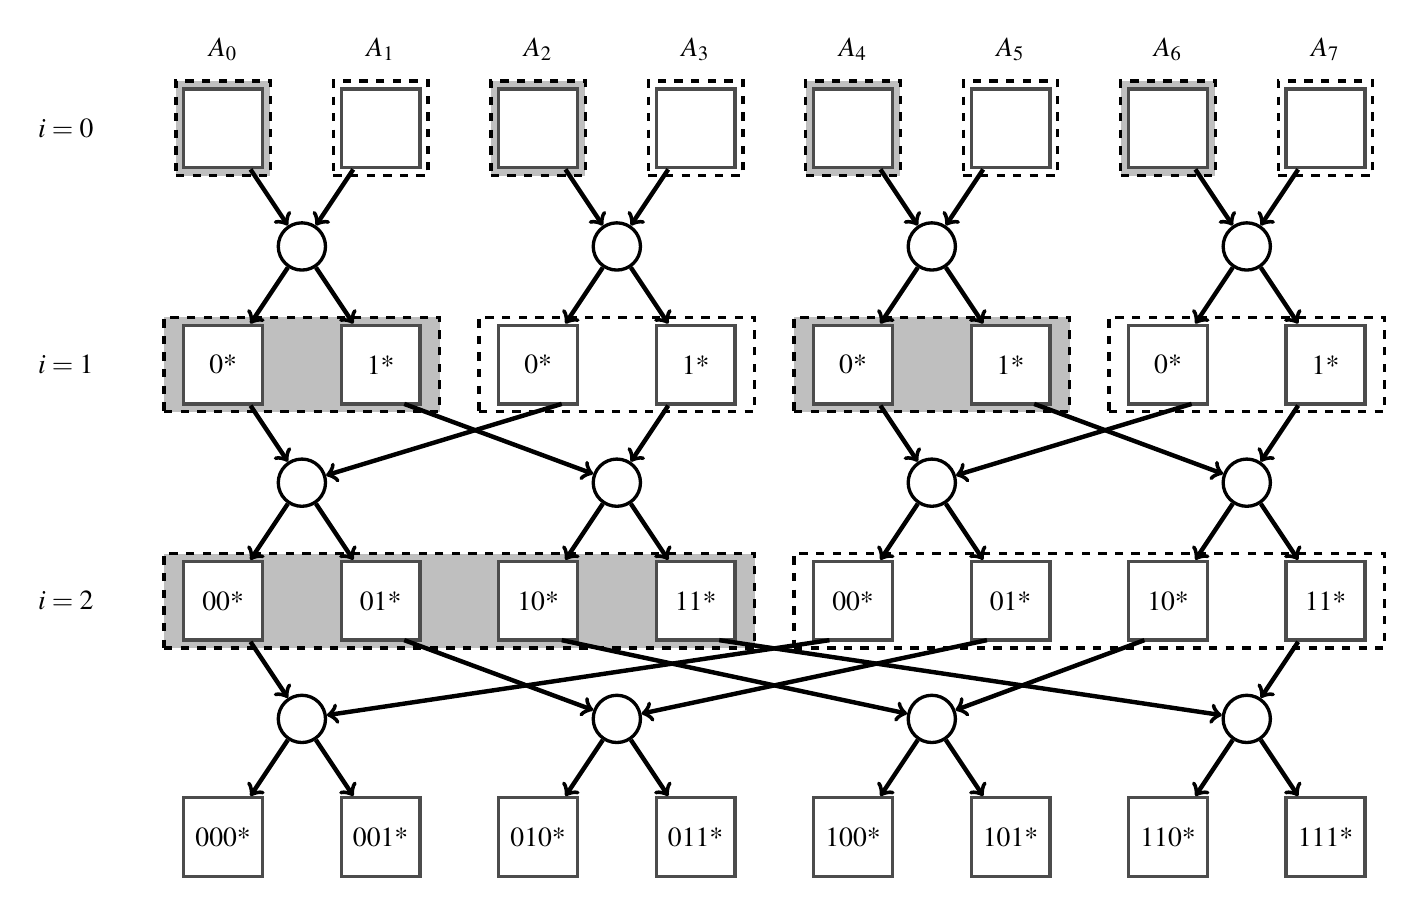
\begin{tikzpicture}
[
sq/.style={rectangle, draw=black!70, fill=white, very thick, minimum height=1cm, minimum width = 1cm},
textbox/.style={rectangle, draw=white, fill=white, very thick, minimum height=2.5cm},
box1/.style={rectangle, draw=black,dashed, fill=white, very thick, minimum height=1.2cm, minimum width=1.2cm},
box4/.style={rectangle, draw=black,dashed, fill=gray!50, very thick, minimum height=1.2cm, minimum width=1.2cm},
box2/.style={rectangle, draw=black,dashed, fill=white, very thick, minimum height=1.2cm, minimum width=3.5cm},
box5/.style={rectangle, draw=black,dashed, fill=gray!50, very thick, minimum height=1.2cm, minimum width=3.5cm},
box3/.style={rectangle, draw=black,dashed, fill=white, very thick, minimum height=1.2cm, minimum width=7.5cm},
box6/.style={rectangle, draw=black,dashed, fill=gray!50, very thick, minimum height=1.2cm, minimum width=7.5cm},
merge/.style={circle, draw=black, fill=white, very thick, minimum size=6mm},
myarrow1/.style={single arrow, draw=black, fill=black, 
      minimum width = 1mm, single arrow head extend=1mm,
      minimum height=1cm},
myarrow2/.style={single arrow, draw=red, fill=red, 
      minimum width = 1mm, single arrow head extend=1mm,
      minimum height=1.3cm},
myarrow3/.style={single arrow, draw=blue, fill=blue, 
minimum width = 0.09cm, single arrow head extend=0.05cm,
minimum height=0.7cm},
textbox/.style={rectangle, draw=white, fill=white, thick, minimum height=0.2cm},
]

\node at (0,6) [textbox] (t0) {$A_0$};
\node at (2,6) [textbox] (t0) {$A_1$};
\node at (4,6) [textbox] (t0) {$A_2$};
\node at (6,6) [textbox] (t0) {$A_3$};
\node at (8,6) [textbox] (t0) {$A_4$};
\node at (10,6) [textbox] (t0) {$A_5$};
\node at (12,6) [textbox] (t0) {$A_6$};
\node at (14,6) [textbox] (t0) {$A_7$};
\node at (-2,5) [textbox] (t0) {$i=0$};
\node at (-2,2) [textbox] (t0) {$i=1$};
\node at (-2,-1) [textbox] (t0) {$i=2$};

\node at (0,5) [box4] (b4) {} ;
\node at (0,5) [sq] (sq11) {};
\node at (2,5) [box1] (b4) {} ;
\node at (2,5) [sq] (sq12) {};
\node at (4,5) [box4] (b4) {} ;
\node at (4,5) [sq] (sq13) {};
\node at (6,5) [box1] (b4) {} ;
\node at (6,5) [sq] (sq14) {};
\node at (8,5) [box4] (b4) {} ;
\node at (8,5) [sq] (sq15) {};
\node at (10,5) [box1] (b4) {} ;
\node at (10,5) [sq] (sq16) {};
\node at (12,5) [box4] (b4) {} ;
\node at (12,5) [sq] (sq17) {};
\node at (14,5) [box1] (b4) {} ;
\node at (14,5) [sq] (sq18) {};

\node at (1,2) [box5] (b4) {} ;
\node at (0,2) [sq] (sq21) {0*};
\node at (2,2) [sq] (sq22) {1*};
\node at (1,3.5) [merge] (c11) {};
\draw[->,black, ultra thick]  (c11) -- (sq21);%(0.5,6.7) -- (1,6);
\draw[->,black, ultra thick]  (c11) -- (sq22);

\node at (5,2) [box2] (b4) {} ;
\node at (4,2) [sq] (sq23) {0*};
\node at (6,2) [sq] (sq24) {1*};
\node at (5,3.5) [merge] (c12) {};
\draw[->,black, ultra thick]  (c12) -- (sq23);
\draw[->,black, ultra thick]  (c12) -- (sq24);


\node at (9,2) [box5] (b4) {} ;
\node at (8,2) [sq] (sq25) {0*};
\node at (10,2) [sq] (sq26) {1*};
\node at (9,3.5) [merge] (c13) {};
\draw[->,black, ultra thick]  (c13) -- (sq25);
\draw[->,black, ultra thick]  (c13) -- (sq26);

\node at (13,2) [box2] (b4) {} ;
\node at (12,2) [sq] (sq27) {0*};
\node at (14,2) [sq] (sq28) {1*};
\node at (13,3.5) [merge] (c14) {};

\draw[->,black, ultra thick]  (c14) -- (sq27);
\draw[->,black, ultra thick]  (c14) -- (sq28);
\draw[->,black, ultra thick]  (sq11) -- (c11);
\draw[->,black, ultra thick]  (sq12) -- (c11);
\draw[->,black, ultra thick]  (sq13) -- (c12);
\draw[->,black, ultra thick]  (sq14) -- (c12);
\draw[->,black, ultra thick]  (sq15) -- (c13);
\draw[->,black, ultra thick]  (sq16) -- (c13);
\draw[->,black, ultra thick]  (sq17) -- (c14);
\draw[->,black, ultra thick]  (sq18) -- (c14);

\node at (3,-1) [box6] (b4) {} ;
\node at (0,-1) [sq] (sq31) {00*};
\node at (2,-1) [sq] (sq32) {01*};
\node at (1,0.5) [merge] (c21) {};
\draw[->,black, ultra thick]  (c21) -- (sq31);
\draw[->,black, ultra thick]  (c21) -- (sq32);
\node at (4,-1) [sq] (sq33) {10*};
\node at (6,-1) [sq] (sq34) {11*};
\node at (5,0.5) [merge] (c22) {};
\draw[->,black, ultra thick]  (c22) -- (sq33);
\draw[->,black, ultra thick]  (c22) -- (sq34);
\node at (11,-1) [box3] (b4) {} ;
\node at (8,-1) [sq] (sq35) {00*};
\node at (10,-1) [sq] (sq36) {01*};
\node at (9,0.5) [merge] (c23) {};
\draw[->,black, ultra thick]  (c23) -- (sq35);
\draw[->,black, ultra thick]  (c23) -- (sq36);
\node at (12,-1) [sq] (sq37) {10*};
\node at (14,-1) [sq] (sq38) {11*};
\node at (13,0.5) [merge] (c24) {};
\draw[->,black, ultra thick]  (c24) -- (sq37);
\draw[->,black, ultra thick]  (c24) -- (sq38);
\draw[->,black, ultra thick]  (sq21) -- (c21);
%\draw[->,black, ultra thick]  (5.4,2) -- (c21);
%\draw[->,black, ultra thick]  (2.6,2) -- (c22);
\draw[->,black, ultra thick]  (sq24) -- (c22);
\draw[->,black, ultra thick]  (sq25) -- (c23);
%\draw[->,black, ultra thick]  (17.8,2) -- (c23);
%\draw[->,black, ultra thick]  (15.6,2) -- (c24); 
\draw[->,black, ultra thick]  (sq28) -- (c24);

\draw[->,black, ultra thick]  (2.3,1.5) -- (c22);%%
\draw[->,black, ultra thick]  (4.3,1.5) -- (c21);%%
\draw[->,black, ultra thick]  (10.3,1.5) -- (c24);%%
\draw[->,black, ultra thick]  (12.3,1.5) -- (c23);%%

\node at (0,-4) [sq] (sq41) {000*};
\node at (2,-4) [sq] (sq42) {001*};
\node at (1,-2.5) [merge] (c31) {};
\draw[->,black, ultra thick]  (c31) -- (sq41);
\draw[->,black, ultra thick]  (c31) -- (sq42);
\node at (4,-4) [sq] (sq43) {010*};
\node at (6,-4) [sq] (sq44) {011*};
\node at (5,-2.5) [merge] (c32) {};
\draw[->,black, ultra thick]  (c32) -- (sq43);
\draw[->,black, ultra thick]  (c32) -- (sq44);
\node at (8,-4) [sq] (sq45) {100*};
\node at (10,-4) [sq] (sq46) {101*};
\node at (9,-2.5) [merge] (c33) {};
\draw[->,black, ultra thick]  (c33) -- (sq45);
\draw[->,black, ultra thick]  (c33) -- (sq46);
\node at (12,-4) [sq] (sq47) {110*};
\node at (14,-4) [sq] (sq48) {111*};
\node at (13,-2.5) [merge] (c34) {};
\draw[->,black, ultra thick]  (c34) -- (sq47);
\draw[->,black, ultra thick]  (c34) -- (sq48);
\draw[->,black, ultra thick]  (sq31) -- (c31);%

\draw[->,black, ultra thick]  (7.7,-1.5) -- (c31);
\draw[->,black, ultra thick]  (2.3,-1.5) -- (c32);
\draw[->,black, ultra thick]  (9.7,-1.5) -- (c32);
\draw[->,black, ultra thick]  (4.3,-1.5) -- (c33);
\draw[->,black, ultra thick]  (11.7,-1.5) -- (c33);
\draw[->,black, ultra thick]  (6.3,-1.5) -- (c34);

\draw[->,black, ultra thick]  (sq38) -- (c34); %
\end{tikzpicture}
}
\captionsetup{font=small}
\caption{Oblivious random bin assignment with 8 buckets: The circles \textbf{\textbigcircle}\ denote 
the \textsf{MergeSplit} units and the squares \textbf{\large{$\square$}}\ denote buckets. 
The \mergeSplit\ function takes two buckets at level $i$ 
and put them into two consecutive buckets at level $i+1$, based on 
the $(i+1)th$ most significant bit of the random keys assigned to each element of the buckets. 
This figure is replicated from Figure 1 of [5].}
\label{fig:bucketSort}
\end{figure}

\begin{figure}[!h]
\centering
\scalebox{0.5}{
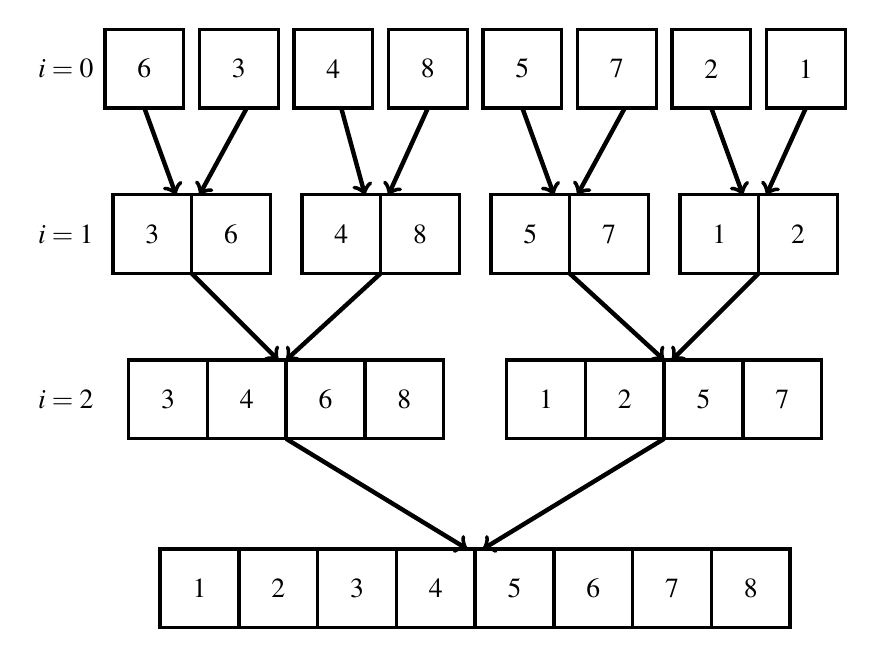
\begin{tikzpicture}
[
sq/.style={rectangle, draw=black!70, fill=white, very thick, minimum height=2cm, minimum width = 2cm},
textbox/.style={rectangle, draw=white, fill=white, very thick, minimum height=2.5cm},
box1/.style={rectangle, draw=black, fill=white, very thick, minimum height=1cm, minimum width=1cm},
merge/.style={circle, draw=black, fill=white, very thick, minimum size=8mm},
myarrow1/.style={single arrow, draw=black, fill=black, 
      minimum width = 1mm, single arrow head extend=1mm,
      minimum height=1cm},
textbox/.style={rectangle, draw=white, fill=white, thick, minimum height=0.2cm},
]

\node at (-1,0) [textbox] (t1) {$i=0$};
\node at (-1,-2.1) [textbox] (t2) {$i=1$};
\node at (-1,-4.2) [textbox] (t3) {$i=2$};

\node at (0,0) [box1] {6};
\node at (1.2,0) [box1] {3};
\node at (2.4,0) [box1] {4};
\node at (3.6,0) [box1] {8};
\node at (4.8,0) [box1] {5};
\node at (6,0) [box1] {7};
\node at (7.2,0) [box1] {2};
\node at (8.4,0) [box1] {1};

\node at (0.1,-2.1) [box1] {3};
\node at (1.1,-2.1) [box1] {6};
\node at (2.5,-2.1) [box1] {4};
\node at (3.5,-2.1) [box1] {8};
\node at (4.9,-2.1) [box1] {5};
\node at (5.9,-2.1) [box1] {7};
\node at (7.3,-2.1) [box1] {1};
\node at (8.3,-2.1) [box1] {2};

\node at (0.3,-4.2) [box1] {3};
\node at (1.3,-4.2) [box1] {4};
\node at (2.3,-4.2) [box1] {6};
\node at (3.3,-4.2) [box1] {8};
\node at (5.1,-4.2) [box1] {1};
\node at (6.1,-4.2) [box1] {2};
\node at (7.1,-4.2) [box1] {5};
\node at (8.1,-4.2) [box1] {7};

\node at (0.7,-6.6) [box1] {1};
\node at (1.7,-6.6) [box1] {2};
\node at (2.7,-6.6) [box1] {3};
\node at (3.7,-6.6) [box1] {4};
\node at (4.7,-6.6) [box1] {5};
\node at (5.7,-6.6) [box1] {6};
\node at (6.7,-6.6) [box1] {7};
\node at (7.7,-6.6) [box1] {8};

\draw[->,black, ultra thick]  (0,-0.5) -- (0.4,-1.6);
\draw[->,black, ultra thick]  (1.3,-0.5) -- (0.7,-1.6);

\draw[->,black, ultra thick]  (2.5,-0.5) -- (2.8,-1.6);
\draw[->,black, ultra thick]  (3.6,-0.5) -- (3.1,-1.6);

\draw[->,black, ultra thick]  (4.8,-0.5) -- (5.2,-1.6);
\draw[->,black, ultra thick]  (6.1,-0.5) -- (5.5,-1.6);

\draw[->,black, ultra thick]  (7.2,-0.5) -- (7.6,-1.6);
\draw[->,black, ultra thick]  (8.4,-0.5) -- (7.9,-1.6);


\draw[->,black, ultra thick]  (0.6,-2.6) -- (1.7,-3.7);
\draw[->,black, ultra thick]  (3,-2.6) -- (1.8,-3.7);
\draw[->,black, ultra thick]  (5.4,-2.6) -- (6.6,-3.7);
\draw[->,black, ultra thick]  (7.8,-2.6) -- (6.7,-3.7);

\draw[->,black, ultra thick]  (1.8,-4.7) -- (4.1,-6.1);
\draw[->,black, ultra thick]  (6.6,-4.7) -- (4.3,-6.1);

\end{tikzpicture}
}
%\captionsetup{font=small}
\caption{Merge sort: always two consecutive chunks of $2^i$ elements from 
level $i$ are merged 
and written to $2^{i+1}$ consecutive memory locations at level $i+1$. 
%This causes 2 random disk-head movements for a single merge.
}
\label{fig:mergeSort}
\end{figure}

\section{De-amortizing bucket oblivious sort.} \label{append:bucketSort} \label{append:bucketLoc}
 An oblivious sorting algorithm sorts an array of elements without leaking information about the relative ordering of the input elements. 
 Recently, Asharov et al.~\cite{bucketSort} presented an oblivious bucket
 sort algorithm that obliviously sorts the input elements in three steps: First, it performs an \emph{Oblivious Random Bin Assignment} (ORBA). ORBA obliviously and uniformly randomly distribute the $N$ input elements and $N$ extra dummy elements into a set of buckets. Each element is assigned to an independent random bucket, and elements are then routed into the buckets obliviously. %Fetching one bucket from disk requires always $\bO(1)$ locality, since the elements of a bucket are always stored in contiguous memory locations. 
 Second, after performing the ORBA, it computes an \emph{Oblivious Random Permutation (ORP)}  which is achieved by scanning the output of ORBA, deleting dummy elements from each bin and then obliviously permuting each bin (either locally or using bitonic sort). Finally, it  sorts the ORP output using any \emph{non-oblivious} comparison-based sort.
 % We can de-amortize bucket sort into $N \log N/\gamma$ rounds of $\bO(\gamma)$ work per round (e.g., for $\gamma = O(\log N)$ the oblivious bucket sort can be completed in $N$ rounds---see Appendix \ref{append:bucketSort} for more details. 
 We use merge sort as the \emph{non-oblivious} sort. Merge-sort is a stable sort (preserves relative ordering of elements). %One merge operation in merge sort has $\bO(1)$ locality. 
 This algorithm takes $\bO(N\log N)$ time (assuming the client can safely store a small number of elements, e.g., for $N=2^{30}$ the client needs to store $1024$ elements locally). 
 \newline
 \underline{\textbf{De-amortizing Oblivious Random Bin Assignment}}
There are a total of $B= \frac{2{\cdot}N}{Z}$ buckets, where $Z$ is the size of the
buckets. In the bucket sort algorithm a total of $\log B$ levels of \mergeSplit s
(see Figure \ref{fig:bucketSort}) take place. 
And in each of these levels $\frac{B}{2}$ \mergeSplit s happen.
That is, overall $\frac{B}{2} {\cdot} \log B$ \mergeSplit s takes place. 
In, other words, one can de-amortize the oblivious random bin assignment 
in $\frac{B/2 {\cdot} \log B}{\gamma}$ steps, doing $\gamma$ \mergeSplit s in each step.
\newline
\underline{\textbf{De-amortizing Oblivious Random Permutation (ORP)}}
For this step the client fetches one bucket, 
removes all the dummy elements (which comes at the end) and locally permute the
non-dummy elements. 
As there are $B$ buckets, this step can be de-amortized
into at most of $B$ steps. If we permute $\gamma$ buckets in a single step then
ORP can be performed in $\frac{B}{\gamma}$ steps. 
\newline
\underline{\textbf{De-amortizing Non Oblivious sort}} 
We have used iterative merge sort in this step,
which can be de-amortized. 
For an input array of $N$ items merge sort runs in $\log N$ levels, 
and does $N$ work (compares) per level (see Figure \ref{fig:mergeSort}). 
The $ith$ level sorts every chunk of 
$2^i$ elements. Or in other words, the $ith$ level merges two consecutive 
sorted chunk of $2^{i-1}$ elements. If we de-amortized merge sort doing 
$\gamma$ work (merges) per step, it will require $\frac{N \log N}{\gamma}$ 
steps to finish the merge sort. \newline
%If $\gamma = {\log N$, the merge sort takes $N$ rounds
%to sort $N$ items. 
\underline{\textbf{Locality of bucket oblivious sort.} }
\textbf{(i)} Fetching a bucket from the disk requires one I/O, 
since the elements of the bucket are stored in contiguous memory locations.
Fetching two buckets during a single \mergeSplit\ will cause two I/Os. 
The outputs are written to two consecutive buckets, causing only one I/O. 
Hence, we can say the one \mergeSplit\ of {oblivious random 
bin assignment} (ORBA) causes three I/Os, or has $\bO(1)$ locality. 
Overall, there are $\frac{B}{2}{\cdot} \log B$ \mergeSplit s, and hence
$\bO(B \log B) < \bO(N \log N)$ locality.
\textbf{(ii)} For the ORP, fetching one bucket causes one I/O. 
The permuted elements are written back 
to consecutive memory locations, which causes another I/O. 
There are $B$ buckets, hence the ORP causes $2{\cdot} B$ 
random disk-head movement in total. 
So, one step of ORP has $\bO(1)$ locality and overall ORP has $\bO(B)$ 
locality. \textbf{(iii)} During a particular merge in merge sort, 
two consecutive chunks of $2^i ~(0 \leq i \leq (\log N-1))$ elements are fetched, 
sorted and the merged output is written back to $2^{i+1}$ consecutive 
memory locations. In this way, one merge costs two I/Os. 
There are $\log N$ levels, where the level $i$ requires 
$2^{{\log N}}$ random I/Os; taking summation of all these we get merge sort's 
locality to be $\bO(N)$. This makes locality of bucket oblivious sort to be 
$\bO(N \log N)$.


\section{Definitions of I/O efficiency metrices.} \label{append:metrics}

\begin{definition}[Search locality]
\neww{The search locality (or locality) of an SE scheme (static or dynamic) that uses HDDs as the underlying storage medium is defined as the total number of non-contiguous memory regions read during a search operation.  } 
\end{definition}

\begin{definition}[Update locality]
\neww{The update locality of a DSE scheme that uses HDDs as the underlying storage medium is defined as the total number of non-contiguous memory regions accessed during an update operation.  } 
\end{definition}

\begin{definition}[Read efficiency]
\neww{The read efficiency of an SE scheme that uses HDDs as the underlying storage medium is defined as the ratio of total number of memory locations read over the number of memory locations read pertaining to the results during a search operation.}
\end{definition}

 %All of these three metrices are relevant for schemes that use HDDs as the storage medium.

\begin{definition}[Page efficiency]
The page efficiency of an SE scheme that uses SSDs as the underlying storage medium is defined as the ratio of the total number of memory pages read for encrypted result during a search over the number of memory pages that would have been read for the plaintext result.
\end{definition}

\begin{definition}[Update efficiency]
\neww{The page efficiency of a DSE scheme that uses SSDs as the underlying storage medium is defined as the number of memory pages accessed during an update operation.}
\end{definition}

\begin{definition}[Update asymptotic cost]
\neww{The update asymptotic cost of a DSE scheme that uses either HDDs or SSDs as the underlying storage medium is defined as the asymptotic cost of a single insert or a delete.}
\end{definition}

\begin{definition}[Space overhead]
\neww{The space overhead of an SE scheme that uses either HDDs or SSDs as the underlying storage medium is defined as the ratio of the total space used to store the encrypted database over the size of the plaintext database.}
\end{definition}

\neww{Search locality is commonly referred as just \emph{locality}. \emph{Read efficiency}, 
\emph{locality}, \emph{page efficiency} and \emph{space overhead} are applicable for both SSEs and DSEs, while \emph{update locality} and \emph{update asymptotic} cost are applicable only for DSEs.}


\begin{figure}[!h]
	\begin{mdframed}
		\setlength{\itemindent}{-.3 in}
		Let {\sf $\Gamma$ = (\Setup, \Search, \texttt{DecryptAll})} be a result-hiding, static searchable encryption scheme.
 %\begin{multicols}{2}
  \underline{$(K,\sigma , EDB) \leftarrow \Setup(\lambda,N)$}
		\begin{algorithmic}[1]
		\State Let $\ell \gets \lfloor \log N \rfloor$
		\FFor{$i=0\ldots \ell$} Set empty index $EDB_i$ of size $2^i$
			\State $EDB$  $\gets \{EDB_0, \ldots, EDB_\ell\}$
			\State Set $K,\sigma$ to be empty vectors
			\State \Return $EDB$ to Server and $(K,\sigma)$ to Client \newline
		\end{algorithmic}
		%\underline{$(st_{\sf C},\mathcal{I})\leftarrow${\sf Update}$(op,w,id,st_{\mathcal{C}})$}
		\underline {$(K, \sigma ; EDB) \leftrightarrow$ {\Update$(K,op,w,id,\sigma;EDB)$}}
		\begin{algorithmic}[1]
			\item[Server:]
			\State Find the minimum $j$ such that $EDB_j = \emptyset$
			\State Send to client $EDB_0,\dots,EDB_{j-1}$
			
			\item[Client:]
			\State Set $A \leftarrow \emptyset$
			\For{$i=0, \dots, j-1$}
			\State $A\leftarrow$ $A\; \cup$ {\sf $\Gamma$.\texttt{DecryptAll}}($K[i],\sigma[i],EDB_i$)
			\State $K[i] \leftarrow \bot$, $\sigma[i]\leftarrow \bot$
			\EndFor
			\State {\small $(K[j],\sigma[j],EDB_A) \leftarrow$} {\sf $\Gamma$.\Setup} {\small ($A \cup (w,id,op)$)}
				\State \Return $EDB_A$ to server
			\item[Server:]
			\State Set $EDB_j \leftarrow EDB_A$
			\For{$i=0, \dots, j-1$}
			\State Set $EDB_i \leftarrow \emptyset$
			\EndFor\newline
		\end{algorithmic}
		\underline{$DB(w) \leftrightarrow \textsf{\Search}(K,q,\sigma ; EDB)$}
		\begin{algorithmic}[1]
			\item[Client $\leftrightarrow$ Server:]
			\State $\mathcal{X}\leftarrow\emptyset$.
			\For{all $i$ such that $EDB_i\neq \emptyset$}
			\State Let $\mathcal{X}_i \leftrightarrow$ {\sf $\Gamma$.\Search}($K[i],q,\sigma[i]; EDB_i$)
			\State $\mathcal{X}\leftarrow \mathcal{X} \cup \mathcal{X}_i$
			\EndFor
			\State Send $\mathcal{X}$ to the Client
			\item[Client:]
			%\State Decrypt entries of $\mathcal{X}$ with $K$ and parse them as $(id,op)$
			\State $DB(w) \leftarrow \{id\; | \; (w,id,add)\in \mathcal{X} \land (w,id,del) \not\in \mathcal{X}\}$
			\State \Return $DB(w)$
			%\State \textbf{return} $(\mathcal{X},st_{\mathcal{C}}',\mathcal{I}')$.
		\end{algorithmic}
  %\end{multicols}
	\end{mdframed}
	%\vspace{-0.3cm}
	\caption{{\sf SD}$_a$: from static to dynamic (optimized version).\cite{SDa}}
	%\vspace{-.2cm}
	\label{fig:Scheme1}
\end{figure}

\section{\SDa[$\cdot$]: Details and efficiency proofs}\label{append:SDalocProofs}

The pseudocode of the optimized version of \SDa[$\cdot$] is presented in Figure \ref{fig:Scheme1}. Below we prove a theorem that says, when a \emph{locality-aware} 
static SE scheme $\Gamma$ instantiated with \SDa[$\cdot$] to produce a \emph{locality-aware} DSE scheme  \SDa[$\cdot$], it retains the original \emph{space-overhead} of $\Gamma$, but for \emph{read-efficiency} and \emph{locality} an additional factor of $\log N$ is introduced as each of $\log N$ indexes are queried separately.  

%\begin{restatable}{theorem}{SDaLoc}\label{thm:SDaLoc}
\begin{theorem}\label{thm:SDaLoc}
Assuming a database of size $N$, and a locality-aware static SE scheme $\Gamma$ 
with $\bO(S)$ space overhead, $\bO(R)$ {search} read-efficiency, 
and $\bO(L)$ {search} locality,
\SDa$[\Gamma]$ has $\bO(S)$ space overhead, $\bO(R+ \log N)$ 
{search} read-efficiency, $\bO(L+\log N)$ {search} locality.% ,  and $\bO(\log N)$ update locality. 
\end{theorem}
%\end{restatable}
%\vspace{-0.3cm}
%\noindent\textit{Proof.}
%\end{theorem}
\begin{proof}\label{thm:SDaLocProof}
 %See Appendix \ref{append:SDalocProofs}
%\SDaLoc* 
%\noindent\textit{Proof.}
\new{In \SDa[$\Gamma$], at most ${\log{N}}$ indices
are created for a database of size $N$. 
%Without loss of generality, 
%we will be using $\log{N}$ instead of $\ceil{\log{N}}$ in the rest of our proof.  
The $k$th index in \SDa[$\Gamma$] is an instance of the static 
SE scheme $\Gamma$ that stores $2^k$ elements. 
\newline 
%\newline
\noindent{\textbf{Space overhead.}} 
%Hence, each individual index in \SDa[$\Gamma$] 
Space overhead of $\Gamma$ is $\bO(S)$; i.e. 
the space complexity is $\bO(S \cdot N)$. %because $\Gamma$ has space overhead \bO(S)$. 
%if $\Gamma$ needs $\bO{(S{\cdot}N)}$ space, 
%then 
Hence, the total space required by \SDa[$\Gamma$] (for a positive constant $c$) is:  
%\begin{align*}
 $c \cdot (S{\cdot}2^0 + S{\cdot}2^1 + \ldots + S{\cdot}2^{\log N -1}) \leq  c{\cdot}S{\cdot}N =  \bO(S{\cdot}N)$

Which incurs $\bO(S)$ \emph{space overhead} for \SDa[$\Gamma$].
\newline%\newline
\noindent{\textbf{Search read efficiency.}} Let us assume keyword $w$ is 
associated to $n_w$ results. 
Because, $\Gamma$ has $\bO(R)$ \emph{search read efficiency}, 
during a search query of $w$, $\Gamma.\Search(K,w,\sigma;EDB)$ 
returns $\bO(R{\cdot}n_w)$ entries. 
%and $\bO(L)$ search locality respectively.
Now, in \SDa[$\Gamma$], those $n_w$ results can be distributed into $\log N$ indexes. 
%(during the updates and local merges). %for \SDa[$\Gamma$]. 
Let us assume that $EDB_k$ has $a_{w_k}$ entries, 
i.e. $0 \leq a_{w_k} \leq a_{w}~~\forall k \in \{0,\ldots,(\log N -1)\}$,
and $n_w = a_{w_0}+a_{w_1}+\ldots+a_{w_{(\log N-1)}}$. 
But, for every $k$th index $EDB_k$, 
the corresponding keyword dictionary (i.e. $EDB_k.\Dict$) 
is queried as well to get the keyword counter values for $w$. 
Hence, total amount of data read for is $EDB_k$ is $\bO(R{\cdot}a_{w_k} + 1)$,
 In \SDa[$\Gamma$], the search happens individually in every index by calling $\Gamma.\Search$.
% Hence the $k$th index returns $\bO(R{\cdot}{a_{w_k}}+1)$ entries. 
Taking the summation 
 of the total data read from all the indexes and dictionaries we get (for a constant $c$):
%\begin{align*}
 $c{\cdot}((R{\cdot}a_{w_0} +1 )+ (R{\cdot}a_{w_1}+1) + \ldots + (R{\cdot}a_{w_{\log N -1}}+1))
%\intertext{\hspace{3cm}$c$ being a constant}
%=& y{\cdot}R{\cdot}(a_{w_0} + a_{w_1} + \ldots +a_{w_{(\log N -1)}}) \\
=  c{\cdot}(R{\cdot}n_w +\log{N})  = \bO(R{\cdot}n_w + \log N)$
%\end{align*} 
which results into \emph{search read efficiency} to be
$\bO(R + \frac{\log N}{n_w})$  i.e.  $\bO(R+\log N)$
\newline %\newline
\noindent{\textbf{Search locality.}} A search query for keyword $w$ in $\Gamma$ causes $\bO(L)$ random 
disk head movements, as $\Gamma$ has $\bO(L)$ \emph{search locality}. 
Let us assume, for each $EDB_k$ in \SDa[$\Gamma$], the disk head moves $L_k$ times 
(which is at most $a_{w_k}$, if $\Gamma$ has worst case locality). So, disk head moves a total of 
$\Sigma_{0 \leq k \leq (\log N -1)} L_k = c{\cdot}L$ times (for some constant $c$). %which is at most $n_w$, if $\Gamma$ 
%has worst case locality.
%But $\Gamma$ has locality $\bO(L)$. 
Moreover, for each access to the dictionaries the disk head moves once, 
causing an extra $\log N$ random disk head movements. 
Hence, in total, \SDa[$\Gamma$] has $(c\cdot L + \log N )$  i.e. $\bO(L + \log N)$ locality.
}
\end{proof}

We have discussed about the potential static SE candidates in 
section \ref{sec:SDalocality}. Here, we will choose \SDa[\OneChoice] 
to explain the locality and read-efficiency as stated in the Theorem \ref{thm:SDaLoc} above.
 %,and on \SDa~with \Tethys, denoted \SDa[\Tethys].
The $i^{th}$ index of \SDa$[\OneChoice]$ stores the
real $2^i$ elements across $\ceil{{2^i}/{\log 2^i \log \log 2^i}}$ bins.
 During a search, each index is searched by calling 
\OneChoice.\Search, with locality $\bO(1)$, 
as \emph{locality} of \OneChoice\ is $\bO(1)$.
Since there are at most $\log N$ non-empty indexes: \new{$EDB_0.\Ind$, $EDB_1.\Ind$ \ldots $EDB_{\log N -1}.\Ind$, 
and the corresponding $\log N$ dictionaries: $EDB_0.\Dict$, $EDB_1.\Dict$ \ldots $EDB_{\log N-1}.\Dict$, the total number of required I/Os is $2\log N$, i.e.} search locality for \SDa$[\OneChoice]$ is $\bO(\log N)$. 
Read-efficiency for \SDa$[\OneChoice]$ is $\bO(\log N \log\log N + \log N)$; \new{the extra $\log N$ factor is added as $\log N$ keyword counter information is fetched from the $\log N$ dictionaries}. 
The transformation preserves the storage overhead of \OneChoice, which is optimal. %($\bO(N)$). 
Finally, regarding updates, the amortized update overhead is $\bO(\log N)$ as the setup time of \OneChoice~ is linear, and the update locality is $\bO(\log N)$ as at most $\log N$ indexes are fetched. Table~\ref{table:SDaLoc} provides different instantiations of the \SDa[$\cdot$] transformation with \emph{locality-aware} static SE schemes. We highlight that the amortized update overhead for \TwoChoice\ and \NlogN\ is $\bO(\log^2 N)$ since their setup time is $\bO(N \log N)$. 


Below we prove another theorem, for \emph{page-efficient} static SE schemes instantiated with \SDa[$\cdot$].

\begin{theorem}\label{thm:SDaPE}
Assuming a database of size $N$, and a page efficient static SE scheme $\Gamma$ 
with $\bO(P)$ page efficiency, and $\bO(S)$ space overhead,
\SDa$[\Gamma]$ has 
$\bO(S)$ space overhead, and $\bO(P + \log N)$ worst case search page efficiency. 
%\tblue{what about update efficiency?}.
\end{theorem}
%\end{theorem}
%\noindent\textit{Proof.} \tblue{See Appendix \ref{thm:SDaPEProof}}
%\vspace{-0.3cm}
\begin{proof}
\new{In \SDa[$\Gamma$], at most ${\log{N}}$ indices
are created for a database of size $N$. The $k$th index in \SDa[$\Gamma$] 
stores $2^k$ elements. 
\newline %\newline
\noindent{\textbf{Space overhead.}}
For a database with $N$ entries $\Gamma$ has $\bO(S)$ 
space overhead, i.e. it uses $\bO(\frac{S{\cdot}N}{p})$ pages,
where $p$ is the page size.
The total space required by \SDa[$\Gamma$] can be calculated in a similar fashion
to Theorem \ref{thm:SDaLoc}, i.e. 
%\begin{align*}
$c{\cdot}(\frac{S}{p}{\cdot}2^0 + \frac{S}{p}{\cdot}2^1 + \ldots \\
+ \frac{S}{p}{\cdot}2^{\log N -1}) \leq  c \cdot \frac{S}{p}{\cdot}N = \bO(S{\cdot}N)$
; which incurs $\bO(S)$ \emph{space overhead}.
\newline %\newline
\noindent{\textbf{Search page efficiency.}} 
$\Gamma$ has $\bO(P)$ \emph{search page efficiency}. Let us assume keyword $w$ has $n_w$ results. 
During a search query of $w$, $\Gamma.\Search(K,w,\sigma;EDB)$ returns $\bO(\frac{{P{\cdot}n_w}}{p})$ 
pages. % (for an integer constant $y$), 
%and it causes $z{\cdot}L$ random disk head movements, 
%and $\bO(L)$ search locality respectively.
The $n_w$ results can get distributed in $\log N$ indexes 
in \SDa[$\Gamma$]. Let us assume that $EDB_k$ has $a_{w_k}$ entries, 
for $0 \leq k \leq (\log N-1)$, i.e. $n_w$ = $a_{w_0}$$+a_{w_1}+$$\ldots+$$a_{w_{(\log N-1)}}$.
 In \SDa[$\Gamma$], the search happens individually in every index by calling $\Gamma.\Search$.
 Hence the $k$th index returns $\bO(\frac{P{\cdot}{a_{w_k}}}{p}+2)$ pages. 
 The extra 2 pages are returned 
 because in worst case the starting and ending point of the result list might not be page aligned. 
 Moreover, another page is fetched during querying the 
 keyword dictionary. Taking summation of all we get, (for some constant $c$):
%\begin{align*}
$ c{\cdot}(\frac{P{\cdot}a_{w_0}}{p} +3)+ (\frac{P{\cdot}a_{w_1}}{p} +3) + \ldots + (\frac{P{\cdot}a_{w_{\log N -1}}}{p} +3)\\
%=& \frac{P}{p}{\cdot}(r_0 + r_1 + \ldots +r_{(\log N -1)}) + 3{\cdot}\log N \\
=  \frac{c \cdot P}{p}{\cdot}n_w + 3 {\cdot} \log N $
%\end{align*} 
%The $\log N$ dictionaries are queried to get the keyword counters, that results 
%into fetching additional $\log N$ pages. Hence the total number of pages fetched are
%$\frac{y{\cdot}P}{p}{\cdot}r + 2 {\cdot} \log N$ + $\log N$, 
which makes the 
\emph{search page efficiency} to be $c\cdot (P + \frac{3{\cdot}\log N}{n_w/p})$ i.e. $\bO(P + \log N)$.}
\end{proof}

Static \emph{page-efficient} schemes, e.g., \Tethys\ \cite{BFF21} and \NlogN\ \cite{onechoice} can be instantiated with \SDa\. \Tethys\ fetches two pages from the server during search, hence it offers $\bO(1)$ \emph{search page efficiency}. The page efficiency of \SDa[\Tethys] will be $\bO(\log N)$ since it will require two page accesses per index.   
The amortized update overhead of \SDa[\Tethys] is $\bO(N \log N)$ 
since its setup time is $\bO(N^2)$. 
Similarly, the page efficiency of \SDa[\NlogN] is $\bO(\log N)$, and its amortized update overhead is $\bO(\log^2 N)$, since its page-efficiency is $\bO(1)$ and setup time is $\bO(N \log N)$ respectively. 


\section{Efficiency and security proofs of \LSDd$[\cdot]$} \label{append:proofsSDd}

Below we prove some theorems for our \LSDd[$\cdot$] construction. The theorem statement 
same as that of Theorem \ref{thm:SDaLoc}. The proof follows the similar arguments as well.
In Lemma \ref{lemma:sDdomergeObl} we prove that our \omerge\ scheme is adaptively secure. Lemma \ref{lemma:SDdP2P3} proves that our \omerge\ protocol satisfies properties P2 and P3. Finally, Theorem \ref{thm:SDd} proves that our \LSDd[$\cdot$] scheme is secure against an adaptive adversary.

\begin{theorem}\label{thm:SDdLoc}
\new{Assuming a database of size $N$, and a locality-aware static SE scheme 
$\Gamma \in \{\PiBas,\OneChoice, \TwoChoice,\NlogN\}$ 
with $\bO(S)$ storage overhead, $\bO(R)$ {search} read efficiency, 
and $\bO(L)$ {search} locality,
\LSDd$[\Gamma]$ has $\bO(S)$ storage overhead, $\bO(R+ \log N)$ 
{search} read efficiency, $\bO(L+\log N)$ {search} locality.}
%and $\bO(\log N)$ update locality. 
\end{theorem}
%\end{restatable}

\begin{proof}\label{thm:SDdLocProof}
   \new{ This can proved in a similar way as that of Theorem \ref{thm:SDaLoc}. The only 
    difference is that here we will have an extra constant factor of 3 for \emph{search locality} 
    and \emph{read efficiency}, and a constant factor of 4 for storage.}
\end{proof}


\new{We use the Bucket oblivious sort presented in \cite{bucketSort} and 
oblivious compaction from \cite{compact1} \cite{compact2} in our \omerge\ algorithm. 
These algorithms are proven to be oblivious in the respective works. Hence, we can 
assume the existence of simulators \simosort\ and \simocompact, defined as follows:
\begin{itemize}
    \item \simosort($N$): Takes $N$ as an input and simulates sorting of a list of size length $N$ %by ordering function $f$.
    \item \simocompact($N$): Takes $N$ as input and simulates compaction of a list of length $N$  
\end{itemize}
We also assume that these two simulator work in a de-amortized way, simulating the exact same communication pattern as 
that of the respective real protocols.}
%Additionally, we assume existence oblivious Maps. And we also assume that the observer can not
%distinguish between two encrypted values.



%\SDdomerge* \label{lemma:SDdomergeProof}
%\begin{restatable}{lemma}{SDdomerge}\label{lemma:sDdomergeObl}
\begin{lemma}\label{lemma:sDdomergeObl}
\new{Assuming {$\Gamma \in \{\OneChoice,\TwoChoice,\NlogN\}$} 
is adaptively-secure result-hiding static SE scheme, and assuming the 
 existence of oblivious sort and oblivious compaction, \textup{\omerge} is an oblivious protocol.}
%\tblue{what about update efficiency?}.
\end{lemma}
%\end{restatable}
 \begin{proof}
\new{We construct the simulator for \omerge\, in Figure \ref{alg:simframework}. We leave some empty 
lines in the pseudo-code so that the order of the steps matches to the real \omerge\ 
protocol shown in Figure \ref{alg:framework}. These empty lines are basically the 
local operations done at the client-side, and hence are irrelevant in an indistinguishability proof. 
We need to show that the \omerge\ and \simomerge\ protocols are 
indistinguishable w.r.t. an adversary who can observe the memory access 
patterns at the server. The simulator \simomerge\ maintains the exact 
communication pattern as that of \omerge\ framework. We assume function call with different 
number of parameters are indistinguishable. The dummy entries in the proof can be considered 
to be encryption of all 0s.\newline 
\noindent{\textbf{Line 1:}} Happens at client, so no need to simulate. \newline
\noindent{\textbf{Line 2:}} Both \simomerge\ and \omerge\ initializes $\BUF_1$ and $\BUF_2$ 
of same size; i.e. they are indistinguishable \newline
\noindent{\textbf{Line 3:}} \omerge\ stores real entries from $\OLDER$ and $\OLDEST$ to $\BUF_1$, while \simomerge\ accesses the $\OLDER$ and $\OLDEST$ in the exact same manner as that of \omerge\ but stores $|\OLDER|$+$|\OLDEST|$ number of encryption of 0s in $\BUF_1$. 
The real and the dummy entries are indistinguishable as the adversary can not distinguish between the encryption of real entries vs 
encryption of all 0s. \omerge\ calls the bucket oblivious sort and \simomerge\ calls \simosort($|\OLDER|$+$|\OLDEST|$), with exact same communication pattern,
(i.e. in de-amortized way). Hence, the steps are indistinguishable. \newline
\noindent{\textbf{Line 4:}} Both protocols scan $\BUF_1$ in same order. \omerge\ adds the 
\emph{rank} and $n_w$ values to each entry, while \simomerge\ adds dummy (encryption of 0s) values to each entry. Hence, 
the steps are indistinguishable.  \newline
\noindent{\textbf{Line 5:}} Both \omerge\ and \simomerge\ adds $N'$ dummy entries to $\BUF_1$, hence indistinguishable. \newline
\noindent{\textbf{Line 6:}} \omerge\ calls Bucket oblivious sort \cite{bucketSort}, 
while \simomerge\ calls \simosort($2N'$) on $\BUF_1$, which are indistinguishable.  \newline
\noindent{\textbf{Line 7:}} both protocols have same for loop pattern. \newline
\noindent{\textbf{Line 8:}} Client performs a decryption locally in \omerge, while \simomerge\ accesses the same location 
of $\BUF_1$ and then it does nothing. Hence this step is indistinguishable for an adversary that observes memory 
accesses at the server.   \newline
\noindent{\textbf{Line 9:}} \omerge\ appends a real entry to $\BUF_2$, while \simomerge\ appends a dummy entry to $\BUF_2$. The adversary can not distinguish between the two. \newline
\noindent{\textbf{Line 10-11:}} \omerge\ adds appropriate entries to $\BUF_2$ depending on \emph{rank} value, while the simulator adds encryption of 0s irrespective of the \emph{rank}. The steps are indistinguishable. \newline
\noindent{\textbf{Line 12:}} Happens at the client locally, so no need to simulate.\newline
\noindent{\textbf{Line 13:}} Simulator adds encryption of 0s to $\BUF_2$ \newline
\noindent{\textbf{Line 14-15:}} Both \omerge\ and \simomerge\ append dummy entries to $\BUF_1$. Hence, the steps are indistinguishable to the adversary. \newline
\noindent{\textbf{Line 16:}} Indistinguishable, as \simosort\ is indistinguishable to the real bucket oblivious sort. \newline
\noindent{\textbf{Line 17:}}  Indistinguishable, as both do linear scans. \newline
\noindent{\textbf{Line 18:}} Indistinguishable, as \simocompact\ is indistinguishable to the real oblivious compaction. \newline
\noindent{\textbf{Line 19:}} Indistinguishable, as \simosort\ is indistinguishable to the real bucket oblivious sort. \newline
\noindent{\textbf{Line 20:}} Indistinguishable, as both are doing same assignment. \newline
\noindent{\textbf{Line 21:}} Indistinguishable, as same structure of for loop. \newline
\noindent{\textbf{Line 22:}} Indistinguishable, as \simomerge\ accesses the same memory location as that of \omerge. \newline
\noindent{\textbf{Line 23:}} \omerge\ calls \PiBas.\MAP\ locally at the client, while \simomerge\ generates a random key. The two steps are indistinguishable as output of \PiBas.\MAP\ is indistinguishable from a randomly generated key. \newline
\noindent{\textbf{Line 24-25:}} Indistinguishable, as both do same assignments and both returns $\NEW_i$. \newline
Because each operation of \omerge\ and \simomerge\ is indistinguishable to the adversary, the adversary would not be able to tell
whether it is communicating with the real protocol or the simulator. }
\end{proof}

\begin{figure*}[!h]
\begin{mdframed}
\begin{algorithmic}[1]
 \Statex \hskip-1.5em$\Gamma \in \{\OneChoice,\TwoChoice, \NlogN \}$
\Statex \hskip-1.5em If $\Gamma = \OneChoice$, $N'= 3{\cdot} 2^i,m_i = \ceil{\frac{2^i}{\log 2^i \log \log 2^i}}$,  $\forall level\in \{0 \ldots m_i-1\}$ $b_{level} = 3{\cdot}\log 2^i\log \log 2^i$ and $c_{level} = 0$
\Statex \hskip-1.5em If $\Gamma = \NlogN$, $N'= 2^i{\cdot}\log{(2^i+1)}$, $m_i = (i+1)$,   $\forall level\in \{0 \ldots m_i-1\}$ $b_{level} = 2^{level}$ and $c_{level} = 2^{i-level}$
\Statex \hskip-1.5em If $\Gamma = \TwoChoice$, $N'= z{\cdot} 2^i,m_i = \ceil{\frac{2^i}{(\log \log 2^i) (\log \log \log 2^i)^2}}$,  $\forall level\in \{0 \ldots m_i-1\}$ $b_{level} = z{\cdot}(\log \log 2^i)(\log \log \log 2^i)^2$ and $c_{level} = 0$, $2 \leq z \leq 4$
\end{algorithmic}
\underline {{${\sf NEW}_i$ $ \leftrightarrow$ {$\Gamma$.\simomerge$_i(2^i)$}}}
\begin{algorithmic}[1]
\item[Client $\leftrightarrow$ Server:] %\tpurp{$\Sigma$ s inside the function should be deleted}
\Statex \textcolor{blue}{//** \ \ Phase 1 - Preparing sorted input array\ \   **//}	
\State 
\State Initialize arrays $\BUF_1$ of size $3{\cdot}N'$, and $\BUF_2$ of size $N'$ to be empty\label{fw:siminit}
\State Fill up $\BUF_1$ with encryption of 0s;  call \simosort($|\BUF_1|$)\   \label{fw:simfirstsort}
\State Perform two linear scans (one in reverse and one in correct order) on $\BUF_1$, and modify the entries with new encryption of 0s \label{fw:simtwoscans}
\State Linearly scan $\BUF_1$ and pad with more $N'$ elements as encryption of 0s\label{fw:simpad2}% without leaking the actual list length}
   % \State {$cnt \gets 0$}
   \State {Call \simosort($|\BUF_1|$). Keep first $N'$ elements of $\BUF_1$.}\label{fw:simsecondsort}
  \Statex \textcolor{blue}{//** \ \ Phase 2---Prepare index elements and prepare keyword counters \ \ **//}	
    \For{each $j = 1 \ldots |\BUF_1|$}\label{fw:loop1start}
    \State Simulate Client access to $\BUF_1 [j]$%\tgreen{Happens at Client} %Client decrypts $(w,id,op,rank,n_w) \gets \RND.\Dec(k_{rnd},\BUF_1[j])$\label{fw:dec1} %
      \State %\tgreen{Happens at Client} %Client chooses random {$p \gets^{\$} \{0,1\}^\lambda$}\label{fw:randp}
    \State Append encryption of 0s to  ~$\BUF_{2}$%.\Append(\RND.\Enc(k_{rnd},(\bot,\bot,\bot)))$}\label{fw:simrank0} %\Comment{\tpurp{I want to do p+1 here}}
    %{$\BUF_{2}.\Append(\RND.\Enc(k_{rnd},(\bot,\bot,\bot)))$}\label{fw:rankN0}
    \State 
    \State %\tgreen{Happens at Client}%\tred{$((level,pos),\sigma)\gets\texttt{Map}(P[i][3],w,rank,n_w,\sigma)$}\label{fw:simmap}
  \State Write encryption of 0s at $\BUF_{1}[j]$%(\RND.\Enc(k_{rnd},(\bot, \bot, \bot, \bot, \bot)))$ \label{fw:dec2}
    \EndFor\label{fw:simloop1end}
    \Statex \textcolor{blue}{//** \ \ Phase 3---Add dummies\ \ **//}	%\Comment{this phase adds binsize dummy entries per bin}
    \For{$level= 0 \ldots m_i-1$}\label{fw:simloop2start}
    \State for every $pos \in\{0 \ldots c_{level}\}$ call append encryption of 0s to $\BUF_1$ $b_{level}$ times.%.\Append(\RND.\Enc(k_{rnd},(\bot,\bot,\bot,\bot,\bot)))$   $b_{level}$ times \label{fw:simpadbin}
    \EndFor\label{fw:simloop2end}
     \Statex \textcolor{blue}{//** \ \ Phase 4---Final placement \ \ **//}	
    \State Call \simosort($|\BUF_1|$)\   \label{fw:simthirdsort}
    \State Linearly scan $\BUF_1$, and tag every entry with encryption of 0%, i.e. each entry becomes $(\bot,\bot, \bot,0)$ \label{fw:sim0-1tag}
    \State Call \simocompact($|\BUF_1|$); keep first $N'$ entries%; discard the 0 tags }\label{fw:simcompaction}
    \State Call \simosort($|\BUF_2|$); keep first $2^i$ entries\label{fw:simbuf2sort}
    \State 	\NEW$_i.\Ind$ $\gets$ $\BUF_1$ \label{fw:simnewi} \Comment{elements in each $bin/pos$ is randomly shuffled}
   \For{each $s \in \BUF_2$}\label{fw:dictloopstart}
\State Simulate Client access to $s$%\tgreen{Happens at Client}%Client decrypts $(w, cnt_w) \gets \RND.\Dec(k_{rnd}, s)$\label{fw:dec3}
\State  generate a random $key$ and, encryption of all 0's as $value$
%\State \tred{$(key,value) \gets \simPibas.\MAP()$} \label{fw:simpibasmap}
\State 	\NEW$_i.$\Dict[$key$] $\gets value$\label{fw:simmapdict}
\EndFor\label{fw:simdictloopend}
\State \Return \NEW$_i$
\end{algorithmic}
\end{mdframed}
\caption{\simomerge\ framework of $\Gamma \in \{\OneChoice, \TwoChoice, \NlogN\}$\new{this figure is new}}
\label{alg:simframework}
\end{figure*}

\begin{lemma}\label{lemma:SDdP2P3}
	\new{Assuming $\Gamma \in \{\OneChoice, \TwoChoice, \NlogN \}$ is a secure static SE scheme and existence of an oblivious sort, \textup{\omerge} is \textup{(i)} input-output indistiguishable (\textsf{P2}), and \textup{(ii)} decomposable (\textsf{P3}).}
\end{lemma}
\begin{proof} 
\new{(i) The \omerge\ protocol gets \OLDER\ and \OLDEST\ as inputs. Instead of directly placing the entries of $\OLDEST.\Ind \cup \OLDER.\Ind$ to $\NEW.\Ind$, they are placed in buffer $\BUF_1$ first. Then, bucket oblivious sort is executed on $\BUF_1$ w.r.t the lexicographic order of the keywords (line 3 of Figure \ref{alg:framework}), which completely destroyes any input-output mapping that server saw.
Moreover, three more bucket oblivious sorts are performed on $\BUF_1$ (line 6, 16 and 18 of Figure \ref{alg:framework}) before moving the entries to \NEW.\Ind, which guarantees the property \textsf{(P2)}.}

\new{ii) Property \textsf{P3} of \omerge\ is obvious because all protocols can be decomposed into several assembly instructions. To keep the state of the protocol between different $\gamma$ steps, we can store the variables and intermediate states on some temporary files (to make small memory server), and load them at the beginning of the next step. }
\end{proof}


\neww{Now that Lemma \ref{lemma:sDdomergeObl} and Lemma \ref{lemma:SDdP2P3} are proved, we are ready to prove that our \LSDd[$\cdot$] scheme is adaptively secure. }
\begin{theorem}\label{thm:SDd}
 Assuming {\sf $\Gamma \in \{\OneChoice,\TwoChoice,\NlogN\}$} is an adaptively-secure {result-hiding} static SE scheme, and \textup{$\Gamma$.\omerge} is oblivious (\textsf{P1}) {and input-output indistinguishable (\textsf{P2})}, then \LSDd\textup{[$\Gamma$]} is an adaptively-secure DSE according to \textup{Definition~\ref{def:adpSec}} with $\mathcal{L}^{Updt}(\text{op},w,\text{id}) = \bot$  and 
	$\mathcal{L}^{Srch}(w) = {\textbf{Updates}}(w)$.
 \end{theorem}
%\end{restatable}
%\SDdadapsec* \label{thm:sddadapsec}
\begin{proof} Let ${\sf Sim^{ij}_{\Gamma}} = \{SimSetup^{ij}_{{\Gamma}}, SimSearch^{ij}_{{\Gamma}}\}$ be the simulator for $\Gamma$ for $i\in \{0,\ldots {\log N}\}$
and $j \in \{0,\ldots , 2\}$, i.e. 3 simulators per index level (for {\OLDEST}, {\OLDER}\ and {\OLD}). ${\sf Sim} = \{SimSetup, SimSearch, SimUpdate\}$ 
are the simulators for \LSDd[$\Gamma$]. 

{\sf SimSetup} picks a random key $k_{rnd}$, initializes the matrix $P$ and set $upd_{cnt}$ to 0; it stores all the above to its state $\sigma$. It outputs $EDB=\bot$ to the server. The number of levels, which can be derived from the value of $N$, is leaked, which is same as $\lp^{Stp}$ leakage. Hence, $SimSetup$ is indistiguishable from \LSDd[$\Gamma$].\Setup\ since in both cases the adversary gets to know $N$, and  receives an empty $EDB$.

{\sf SimSearch} derives from search leakage $\lp^{Srch}$ $=$ $\textbf{Updates}(w)$ for queried keyword $w$, which contains all the timestamps pertaining to updates of $w$. We highlight that  \LSDd[$\Gamma$].\Search\ leaks only some bits of the above timestamps that is enough to determine together with $upd_{cnt}$ in which indexes and in which levels those entries now reside and call the corresponding {\sf SimSearch$^{ij}_\Gamma$} simulators in black-box manner---inside an index any encrypted entry can be chosen because of \textsf{P1} and \textsf{P2}. Without \textsf{P2} the {\sf SimSearch$^{ij}_\Gamma$} simulators need to use the exact timestamps in order to return specific entries from the index memory locations. {\sf SimSearch} is indistinguishable from \LSDd[$\Gamma$].\Search, since the adversary in both cases retrieves the same number of entries from each index and $\Gamma$ is secure making {\sf SimSearch$^{ij}_\Gamma$} indistinguishable from the real executions of all $\Gamma.\Search$. 

{\sf SimUpdate} is indistinguishable from \LSDd[$\Gamma$].\Update, it calls all the \simomerge$_i$ simulators (one per level) which take as an input the size of the input $2^i$ and executes the next $\gamma$ steps of \simomerge$_i$ (which can be derived from the $upd_{cnt}$). \new{We already proved that \omerge\ satisfies \textsf{(P3)}.} The simulator after each update has to increase the $upd_{cnt}$ and update its state.  
\end{proof}

\neww{Figure \ref{fig:LSDdEx} shows an elaborated example of \omerge\ steps with an instance of \LSDd[\OneChoice].
}




 \begin{figure*}[!h]
 \centering
 %\scalebox{0.6}
 {
 \begin{subfigure}[t]{0.5\textwidth}
 \centering
 \begin{tikzpicture}
 [
 greenball/.style={circle, draw=black, fill=gray!30, very thick, minimum size=7mm},
 redball/.style={circle, draw=black, fill=white, very thick, minimum size=7mm},
 blueball/.style={circle, draw=blue!40, fill=blue!40, very thick, minimum size=7mm},
 yellowball/.style={circle, draw=yellow!40, fill=yellow!40, very thick, minimum size=7mm},
 dummyball/.style={circle, draw=gray, fill=gray, very thick, minimum size=7mm},
 bin/.style={cylinder, draw=black!70, fill=white, thick, minimum height=2.4cm, minimum width = 1cm, rotate=90},
 textbox/.style={rectangle, draw=white, fill=white, thick, minimum height=1cm},
 myarrow1/.style={single arrow, draw=blue, fill=green, 
       minimum width = 10pt, single arrow head extend=3pt,
       minimum height=10mm}
 ]
 \node at (1.6,-1) [textbox]      (tb1)    {$\OLDEST_{i-1}.\Ind$};
\node at (1,0.5) [bin] (bin1) {};
 \node at (1,0) [greenball]      (ball1)      {$id_1$};
 \node at (1,1) [dummyball]      (d1)      {$~\bot~$};
  \node at (2.3,0.5) [bin] (bin2) {};
  \node at (2.3,0) [dummyball]      (d2)   {$~\bot~$};
  \node at (2.3,1) [redball]      (ball2)    {$id_1$};
  \node at (5.7,-1) [textbox]      (tb1)   {$\OLDER_{i-1}.\Ind$};
  \node at (5,0.5) [bin] (bin1) {};
 \node at (5,0) [dummyball]      (ball3)     {$~\bot~$};
 \node at (5,1) [dummyball]      (d3)      {$~\bot~$};
    \node at (6.3,0.5) [bin] (bin2) {};
  \node at (6.3,0) [redball]      (ball4)    {$id_3$};
  \node at (6.3,1) [greenball]      (ball5)   {$id_2$};
 \end{tikzpicture}
 \captionsetup{justification=centering,font=large} 
 \newsubcaption{$\OneChoice$ example}
 \label{fig:1Cexample}
 \end{subfigure}
 }
 \end{figure*}

 \begin{figure*}[htp]
 \ContinuedFloat
 \centering
 %\scalebox{0.6}
 {
 \begin{subfigure}[t]{0.8\textwidth}
 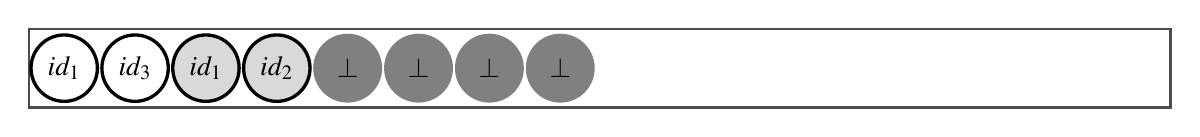
\begin{tikzpicture}
 [
 greenball/.style={circle, draw=black, fill=gray!30, very thick, minimum size=7mm},
 redball/.style={circle, draw=black, fill=white, very thick, minimum size=7mm},
 dummyball/.style={circle, draw=gray, fill=gray, very thick, minimum size=7mm},
 textbox/.style={rectangle, draw=white, fill=white, thick, minimum height=1cm},
 buffer1/.style={rectangle, draw=black!70, fill=white, thick, minimum height=1cm,minimum width=14.5cm}
 ]
  \node at (0,0) [buffer1] (buf) {};
 \node at (-6.8,0) [redball]   (ball1)    {$id_1$};
 \node at (-5.9,0) [redball]   (ball2)                              {$id_3$};
 \node at (-5,0) [greenball]   (ball3)                              {$id_1$};
 \node at (-4.1,0) [greenball]   (ball4)                              {$id_2$};
 \node at (-3.2,0) [dummyball]   (ball5)                              {$~\bot~$};
 \node at (-2.3,0) [dummyball]   (d1)                              {$~\bot~$};
 \node at (-1.4,0) [dummyball]   (d2)                              {$~\bot~$};
 \node at (-0.5,0) [dummyball]   (d3)                              {$~\bot~$};
%\node at (0.3,-1.2) [textbox]      (tb1)                          {$\BUF_1$};
 \end{tikzpicture}
 \captionsetup{justification=justified,font=large}
 \newsubcaption{$\BUF_1$ after oblivious sort w.r.t lexicographic order of keywords.}
 \label{fig:buf1.1}
 \end{subfigure}
 }
 \end{figure*}



 \begin{figure*}[!h]
 \ContinuedFloat
 \centering
%\scalebox{0.6}
{
 \begin{subfigure}[t]{0.8\textwidth}
\centering
   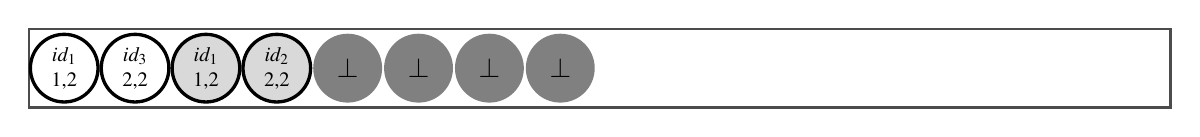
\begin{tikzpicture}
   [
   greenball/.style={circle, draw=black, align=center, fill=gray!30, very thick, minimum size=7mm},
   redball/.style={circle, draw=black,align=center, fill=white, very thick, minimum size=7mm},
   dummyball/.style={circle, draw=gray, align=center, fill=gray, very thick, minimum size=7mm},
   textbox/.style={rectangle, draw=white, fill=white, thick, minimum height=1cm},
   buffer1/.style={rectangle, draw=black!70, fill=white, thick, minimum height=1cm,minimum width=14.5cm},
   ]
 %\node at (0.3,-0.7) [textbox] (tb1) {$\BUF_1$};
 \node at (0,0) [buffer1] (buf) {};
 \node[scale=0.74] at (-6.8,0) [redball]   (ball1)  {$id_1$\\ 1,2};
 \node[scale=0.74] at (-5.9,0) [redball]   (ball2)  {$id_3$\\ 2,2};
 \node[scale=0.74] at (-5,0) [greenball]   (ball3)  {$id_1$\\ 1,2};
 \node[scale=0.74] at (-4.1,0) [greenball]   (ball4) {$id_2$\\ 2,2};
 \node at (-3.2,0) [dummyball]   (ball5)  {$~\bot~$};
 \node at (-2.3,0) [dummyball]   (d1)  {$~\bot~$};
 \node at (-1.4,0) [dummyball]   (d2) {$~\bot~$};
 \node at (-0.5,0) [dummyball]   (d3) {$~\bot~$};
   \end{tikzpicture}
   \captionsetup{justification=centering,font=large}
   \newsubcaption{The first and the second number indicates $rank$ and $n_w$ value respectively. }
   \label{fig:buf1a}
 \end{subfigure}
 }
\end{figure*}


%%%%%%%%%%%%%%%%%%%%%%%%%%%%%THIS ONE
 \begin{figure*}[!h]
 \ContinuedFloat
 \centering
%\scalebox{0.6}
{
 \begin{subfigure}[t]{0.8\textwidth}
\centering
   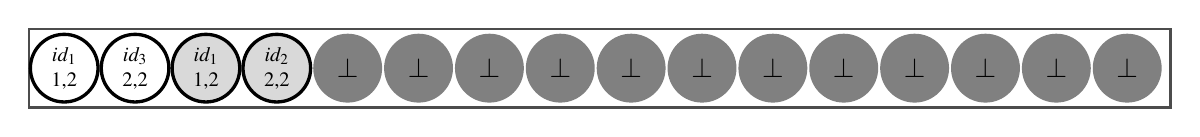
\begin{tikzpicture}
   [
   greenball/.style={circle, draw=black, align=center, fill=gray!30, very thick, minimum size=7mm},
   redball/.style={circle, draw=black,align=center, fill=white, very thick, minimum size=7mm},
   dummyball/.style={circle, draw=gray, align=center, fill=gray, very thick, minimum size=7mm},
   textbox/.style={rectangle, draw=white, fill=white, thick, minimum height=1cm},
   buffer1/.style={rectangle, draw=black!70, fill=white, thick, minimum height=1cm,minimum width=14.5cm},
   ]
 %\node at (0.3,-0.7) [textbox] (tb1) {$\BUF_1$};
 \node at (0,0) [buffer1] (buf) {};
 \node[scale=0.74] at (-6.8,0) [redball]   (ball1)  {$id_1$\\ 1,2};
 \node[scale=0.74] at (-5.9,0) [redball]   (ball2)  {$id_3$\\ 2,2};
 \node[scale=0.74] at (-5,0) [greenball]   (ball3)  {$id_1$\\ 1,2};
 \node[scale=0.74] at (-4.1,0) [greenball]   (ball4) {$id_2$\\ 2,2};
 \node at (-3.2,0) [dummyball]   (ball5)  {$~\bot~$};
 \node at (-2.3,0) [dummyball]   (d1)  {$~\bot~$};
 \node at (-1.4,0) [dummyball]   (d2) {$~\bot~$};
 \node at (-0.5,0) [dummyball]   (d3) {$~\bot~$};
 \node at (0.4,0) [dummyball]   (d4)  {$~\bot~$};
 \node at (1.3,0) [dummyball]   (d5)  {$~\bot~$};
 \node at (2.2,0) [dummyball]   (d6)    {$~\bot~$};
 \node at (3.1,0) [dummyball] (rd7) {$~\bot~$};    
 \node at (4,0) [dummyball]   (d8)   {$~\bot~$};
 \node at (4.9,0) [dummyball]   (d9)   {$~\bot~$};
 \node at (5.8,0) [dummyball]   (d10)   {$~\bot~$};
 \node at (6.7,0) [dummyball]   (d11)   {$~\bot~$};
   \end{tikzpicture}
   \captionsetup{justification=centering,font=large}
   \newsubcaption{$\BUF_1$ after padding each list to power of 2 }
   \label{fig:buf1a}
 \end{subfigure}
 }
%\caption{$\BUF_1$ after different phases}
\end{figure*}

 \begin{figure*}[!h]
 \ContinuedFloat
\centering
 %\scalebox{0.6}
 {
 \begin{subfigure}[t]{0.8\textwidth}
\centering
   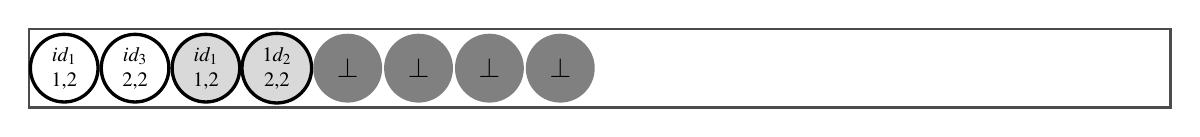
\begin{tikzpicture}
     [
     greenball/.style={circle, draw=black, align=center, fill=gray!30, very thick, minimum size=7mm},
     redball/.style={circle, draw=black,align=center, fill=white, very thick, minimum size=7mm},
     dummyball/.style={circle, draw=gray, align=center, fill=gray, very thick, minimum size=7mm},
     textbox/.style={rectangle, draw=white, fill=white, thick, minimum height=1cm},
     buffer1/.style={rectangle, draw=black!70, fill=white, thick, minimum height=1cm,minimum width=14.5cm},
     ]
  \node at (0,0) [buffer1] (buf) {};
 \node[scale=0.74] at (-6.8,0) [redball]   (ball1)  {$id_1$\\ 1,2};
 \node[scale=0.74] at (-5.9,0) [redball]   (ball2)  {$id_3$\\ 2,2};
 \node[scale=0.74] at (-5,0) [greenball]   (ball5) {$id_1$\\ 1,2};
 \node[scale=0.74] at (-4.1,0) [greenball]   (d1)  {$1d_2$\\ 2,2};
 \node at (-3.2,0) [dummyball]   (d2)  {$~\bot~$};
 \node at (-2.3,0) [dummyball]   (d3)  {$~\bot~$};
 \node at (-1.4,0) [dummyball]   (d2)  {$~\bot~$};
 \node at (-0.5,0) [dummyball]   (d3)  {$~\bot~$};
 \end{tikzpicture}
 \captionsetup{justification=centering,font=large}
 \newsubcaption{$\BUF_1$ at the end of Initialization phase.}
 \label{fig:buf1b}
 \end{subfigure}
 }
 \end{figure*}

 \begin{figure*}[!h]
 \ContinuedFloat
 \centering
 %\scalebox{0.6}
 {
 \begin{subfigure}{0.8\textwidth}
\centering
   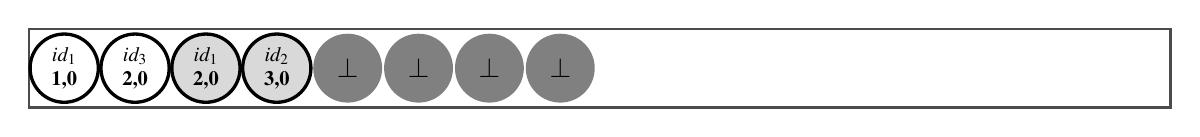
\begin{tikzpicture}
     [
    greenball/.style={circle, draw=black, align=center, fill=gray!30, very thick, minimum size=7mm},
   redball/.style={circle, draw=black,align=center, fill=white, very thick, minimum size=7mm},
     dummyball/.style={circle, draw=gray, align=center, fill=gray, very thick, minimum size=7mm},
     textbox/.style={rectangle, draw=white, fill=white, thick, minimum height=1cm},
     buffer1/.style={rectangle, draw=black!70, fill=white, thick, minimum height=1cm,minimum width=14.5cm},
     ]
  \node at (0,0) [buffer1] (buf) {};
 \node[scale=0.74] at (-6.8,0) [redball]   (ball1)  {$id_1$\\ \tblue{\textbf{1,0}}};
 \node[scale=0.74] at (-5.9,0) [redball]   (ball2)  {$id_3$\\ \tblue{\textbf{2,0}}};
 \node[scale=0.74] at (-5,0) [greenball]   (ball3) {$id_1$\\ \tblue{\textbf{2,0}}};
 \node[scale=0.74] at (-4.1,0) [greenball]   (ball4) {$id_2$\\ \tblue{\textbf{3,0}}};
 \node at (-3.2,0) [dummyball]   (ball5) {$~\bot~$};
 \node at (-2.3,0) [dummyball]   (d1)  {$~\bot~$};
 \node at (-1.4,0) [dummyball]   (d2)  {$~\bot~$};
 \node at (-0.5,0) [dummyball]   (d3)  {$~\bot~$};
%\node at (6.7,0) [dummyball]   (d11)   {$~\bot~$};
   \end{tikzpicture}
   \captionsetup{justification=centering,font=large}
   \newsubcaption{$\BUF_1$ at the end of Phase 1. First number indicates the new bin number. The second number is by default 0 for \OneChoice.}
   \label{fig:buf1c}
 \end{subfigure}
 }
 \end{figure*}

 \begin{figure*}[!h]
 \ContinuedFloat
 \centering
 %\scalebox{0.6}
 {
 \begin{subfigure}[]{0.8\textwidth}
\centering
   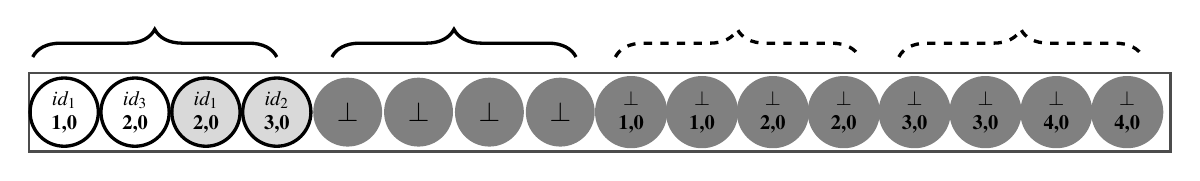
\begin{tikzpicture}
     [
     greenball/.style={circle, draw=black, align=center, fill=gray!30, very thick, minimum size=7mm},
     redball/.style={circle, draw=black,align=center, fill=white, very thick, minimum size=7mm},
     dummyball/.style={circle, draw=gray, align=center, fill=gray, very thick, minimum size=7mm},
     textbox/.style={rectangle, draw=white, fill=white, thick, minimum height=1cm},
     buffer1/.style={rectangle, draw=black!70, fill=white, thick, minimum height=1cm,minimum width=14.5cm},
     ]
  \node at (0,0) [buffer1] (buf) {};
\draw [decorate, decoration = {brace, amplitude = 10pt},very thick] (-7.2,0.7) --  (-4.1,0.7);
\draw [decorate, decoration = {brace, amplitude = 10pt},very thick] (-3.4,0.7) --  (-0.3,0.7);
\draw [decorate, decoration = {brace, amplitude = 10pt},very thick, dashed] (0.2,0.7) --  (3.3,0.7);
\draw [decorate, decoration = {brace, amplitude = 10pt},very thick, dashed] (3.8,0.7) --  (6.9,0.7);
  \node[scale=0.74] at (-6.8,0) [redball]   (ball1)  {$id_1$\\ \tblue{\textbf{1,0}}};
 \node[scale=0.74] at (-5.9,0) [redball]   (ball2)  {$id_3$\\ \tblue{\textbf{2,0}}};
 \node[scale=0.74] at (-5,0) [greenball]   (ball3) {$id_1$\\ \tblue{\textbf{2,0}}};
 \node[scale=0.74] at (-4.1,0) [greenball]   (ball4) {$id_2$\\ \tblue{\textbf{3,0}}};
\node at (-3.2,0) [dummyball]   (ball5) {$~\bot~$};
 \node at (-2.3,0) [dummyball]   (d1)  {$~\bot~$};
 \node at (-1.4,0) [dummyball]   (d2)  {$~\bot~$};
 \node at (-0.5,0) [dummyball]   (d3)  {$~\bot~$};
 \node[scale=0.74] at (0.4,0) [dummyball]   (d4)  {$~\bot~$\\ \tblue{\textbf{1,0}}};
 \node[scale=0.74] at (1.3,0) [dummyball]   (d5)  {$~\bot~$\\ \tblue{\textbf{1,0}}};
 \node[scale=0.74] at (2.2,0) [dummyball]   (d6)  {$~\bot~$\\ \tblue{\textbf{2,0}}};
 \node[scale=0.74] at (3.1,0) [dummyball] (rd7) {$~\bot~$\\ \tblue{\textbf{2,0}}};  
 \node[scale=0.74] at (4,0) [dummyball] (d8) {$~\bot~$\\ \tblue{\textbf{3,0}}};
 \node[scale=0.74] at (4.9,0) [dummyball] (d9) {$~\bot~$\\ \tblue{\textbf{3,0}}};
 \node[scale=0.74] at (5.8,0) [dummyball] (d10)  {$~\bot~$\\ \tblue{\textbf{4,0}}};
 \node[scale=0.74] at (6.7,0) [dummyball]  (d11) {$~\bot~$\\ \tblue{\textbf{4,0}}};
   \end{tikzpicture}
   \captionsetup{justification=centering,font=large}
   \newsubcaption{$\BUF_1$ at the end of Phase 2.Two dummy entries appended for each bin. The braces indicate the bins for the oblivious sort of (next) Phase 3. Two consecutive bucket elements are merged and sorted locally at the client and again written back to two consecutive buckets, as shown in Figure \ref{fig:buf1d} below.}
   \label{fig:buf1d}
 \end{subfigure}
 }
 \end{figure*}

\begin{figure*}[!h]
 \ContinuedFloat
 \centering
 %\scalebox{0.6}
 {
 \begin{subfigure}[]{0.8\textwidth}
\centering
   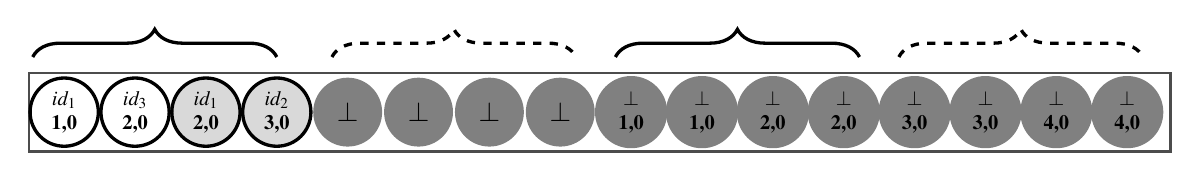
\begin{tikzpicture}
     [
     greenball/.style={circle, draw=black, align=center, fill=gray!30, very thick, minimum size=7mm},
     redball/.style={circle, draw=black,align=center, fill=white, very thick, minimum size=7mm},
     dummyball/.style={circle, draw=gray, align=center, fill=gray, very thick, minimum size=7mm},
     textbox/.style={rectangle, draw=white, fill=white, thick, minimum height=1cm},
     buffer1/.style={rectangle, draw=black!70, fill=white, thick, minimum height=1cm,minimum width=14.5cm},
     ]
  \node at (0,0) [buffer1] (buf) {};
\draw [decorate, decoration = {brace, amplitude = 10pt},very thick] (-7.2,0.7) --  (-4.1,0.7);
\draw [decorate, decoration = {brace, amplitude = 10pt},very thick, dashed] (-3.4,0.7) --  (-0.3,0.7);
\draw [decorate, decoration = {brace, amplitude = 10pt},very thick] (0.2,0.7) --  (3.3,0.7);
\draw [decorate, decoration = {brace, amplitude = 10pt},very thick, dashed] (3.8,0.7) --  (6.9,0.7);
  \node[scale=0.74] at (-6.8,0) [redball]   (ball1)  {$id_1$\\ \tblue{\textbf{1,0}}};
 \node[scale=0.74] at (-5.9,0) [redball]   (ball2)  {$id_3$\\ \tblue{\textbf{2,0}}};
 \node[scale=0.74] at (-5,0) [greenball]   (ball3) {$id_1$\\ \tblue{\textbf{2,0}}};
 \node[scale=0.74] at (-4.1,0) [greenball]   (ball4) {$id_2$\\ \tblue{\textbf{3,0}}};
\node at (-3.2,0) [dummyball]   (ball5) {$~\bot~$};
 \node at (-2.3,0) [dummyball]   (d1)  {$~\bot~$};
 \node at (-1.4,0) [dummyball]   (d2)  {$~\bot~$};
 \node at (-0.5,0) [dummyball]   (d3)  {$~\bot~$};
 \node[scale=0.74] at (0.4,0) [dummyball]   (d4)  {$~\bot~$\\ \tblue{\textbf{1,0}}};
 \node[scale=0.74] at (1.3,0) [dummyball]   (d5)  {$~\bot~$\\ \tblue{\textbf{1,0}}};
 \node[scale=0.74] at (2.2,0) [dummyball]   (d6)  {$~\bot~$\\ \tblue{\textbf{2,0}}};
 \node[scale=0.74] at (3.1,0) [dummyball] (rd7) {$~\bot~$\\ \tblue{\textbf{2,0}}};  
 \node[scale=0.74] at (4,0) [dummyball] (d8) {$~\bot~$\\ \tblue{\textbf{3,0}}};
 \node[scale=0.74] at (4.9,0) [dummyball] (d9) {$~\bot~$\\ \tblue{\textbf{3,0}}};
 \node[scale=0.74] at (5.8,0) [dummyball] (d10)  {$~\bot~$\\ \tblue{\textbf{4,0}}};
 \node[scale=0.74] at (6.7,0) [dummyball]  (d11) {$~\bot~$\\ \tblue{\textbf{4,0}}};
   \end{tikzpicture}
   \captionsetup{justification=centering,font=large}
   \newsubcaption{$\BUF_1$ at an intermediate state during the oblivious merge of Phase 3. This is the output after one of the  calls (out of $2^i$ calls) to \omerge$_i$. Next, two alternative bucket elements are merged and sorted locally, and again written back to two consecutive buckets, as shown in Figure \ref{fig:buf1e} below.}
   \label{fig:buf1d}
 \end{subfigure}
 }
 \end{figure*}




 \begin{figure*}[!h]
 \ContinuedFloat
 \centering
 %\scalebox{0.6}
 {
 \begin{subfigure}[]{0.8\textwidth}
 \centering
   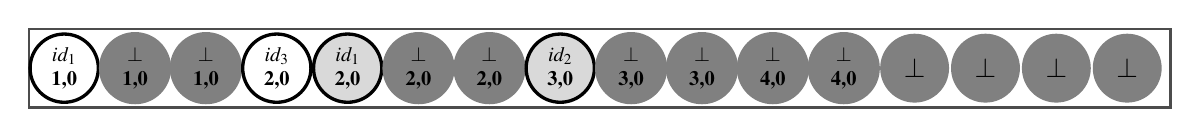
\begin{tikzpicture}
     [
     greenball/.style={circle, draw=black, align=center, fill=gray!30, very thick, minimum size=7mm},
     redball/.style={circle, draw=black,align=center, fill=white, very thick, minimum size=7mm},
     dummyball/.style={circle, draw=gray, align=center, fill=gray, very thick, minimum size=7mm},
     textbox/.style={rectangle, draw=white, fill=white, thick, minimum height=1cm},
     buffer1/.style={rectangle, draw=black!70, fill=white, thick, minimum height=1cm,minimum width=14.5cm},
     ]
  \node at (0,0) [buffer1] (buf) {};
 % \draw [decorate, decoration = {brace, amplitude = 10pt},very thick] (-7.2,0.7) --  (-4.1,0.7);
%\draw [decorate, decoration = {brace, amplitude = 10pt},very thick] (-3.4,0.7) --  (-0.3,0.7);
%\draw [decorate, decoration = {brace, amplitude = 10pt},very thick] (0.2,0.7) --  (3.3,0.7);
%\draw [decorate, decoration = {brace, amplitude = 10pt},very thick] (3.8,0.7) --  (6.9,0.7);
 \node[scale=0.74] at (-6.8,0) [redball]   (ball1)  {$id_1$\\ \tblue{\textbf{1,0}}};
 \node[scale=0.74] at (-5.9,0) [dummyball]   (ball2)  {$~\bot~$\\ \tblue{\textbf{1,0}}};
 \node[scale=0.74] at (-5,0) [dummyball]   (ball3) {$~\bot~$\\ \tblue{\textbf{1,0}}};
 \node[scale=0.74] at (-4.1,0) [redball]   (ball4) {$id_3$\\ \tblue{\textbf{2,0}}};
 \node[scale=0.74] at (-3.2,0) [greenball]   (ball5) {$id_1$\\ \tblue{\textbf{2,0}}};
 \node[scale=0.74] at (-2.3,0) [dummyball]   (d1)  {$~\bot~$\\ \tblue{\textbf{2,0}}};
 \node[scale=0.74] at (-1.4,0) [dummyball]   (d2)  {$~\bot~$\\ \tblue{\textbf{2,0}}};
 \node[scale=0.74] at (-0.5,0) [greenball]   (d3)  {$id_2$\\ \tblue{\textbf{3,0}}};
 \node[scale=0.74] at (0.4,0) [dummyball]   (d4)  {$~\bot~$\\ \tblue{\textbf{3,0}}};
 \node[scale=0.74] at (1.3,0) [dummyball]   (d5)  {$~\bot~$\\ \tblue{\textbf{3,0}}};
 
 \node[scale=0.74] at (2.2,0) [dummyball]   (d6)  {$~\bot~$\\ \tblue{\textbf{4,0}}};
 \node[scale=0.74] at (3.1,0) [dummyball] (rd7) {$~\bot~$\\ \tblue{\textbf{4,0}}};    
 \node at (4,0) [dummyball] (d8) {$~\bot~$};
 \node at (4.9,0) [dummyball] (d9) {$~\bot~$};
 \node at (5.8,0) [dummyball] (d10)  {$~\bot~$};
 \node at (6.7,0) [dummyball]  (d11) {$~\bot~$};
   \end{tikzpicture}
   \captionsetup{justification=centering,font=large}
   \newsubcaption{$\BUF_1$ after the oblivious sort in Phase 3. This is just the state of $\BUF_1$ at the end of Phase 3, but the \omerge\ call may not be done yet. Recall that one call of \omerge\ performs a $\gamma$ number of steps. Those $\gamma$ number of steps may distribute across phases as well. The phases are created only for representation purpose.
   }
   \label{fig:buf1e}
 \end{subfigure}
 }
 \end{figure*}




 \begin{figure*}[!h]
 \ContinuedFloat
 \centering
 %\scalebox{0.6}
 {
 \begin{subfigure}[]{0.8\textwidth}
 \centering
   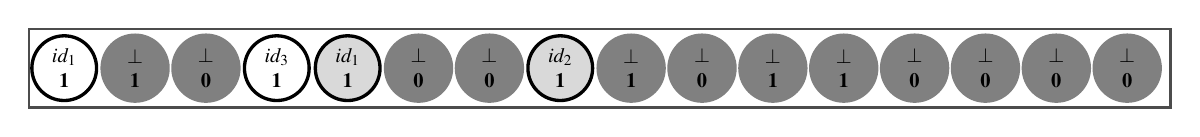
\begin{tikzpicture}
     [
     greenball/.style={circle, draw=black, align=center, fill=gray!30, very thick, minimum size=7mm},
     redball/.style={circle, draw=black,align=center, fill=white, very thick, minimum size=7mm},
     dummyball/.style={circle, draw=gray, align=center, fill=gray, very thick, minimum size=7mm},
     textbox/.style={rectangle, draw=white, fill=white, thick, minimum height=1cm},
     buffer1/.style={rectangle, draw=black!70, fill=white, thick, minimum height=1cm,minimum width=14.5cm},
     ]
  \node at (0,0) [buffer1] (buf) {};
 \node[scale=0.74] at (-6.8,0) [redball]   (ball1)  {$id_1$\\ \tblue{\textbf{1}}};
 \node[scale=0.74] at (-5.9,0) [dummyball]   (ball2)  {$~\bot~$\\ \tblue{\textbf{1}}};
 \node[scale=0.74] at (-5,0) [dummyball]   (ball3) {$~\bot~$\\ \tred{\textbf{0}}};
 \node[scale=0.74] at (-4.1,0) [redball]   (ball4) {$id_3$\\ \tblue{\textbf{1}}};
 \node[scale=0.74] at (-3.2,0) [greenball]   (ball5) {$id_1$\\ \tblue{\textbf{1}}};
 \node[scale=0.74] at (-2.3,0) [dummyball]   (d1)  {$~\bot~$\\ \tred{\textbf{0}}};
 \node[scale=0.74] at (-1.4,0) [dummyball]   (d2)  {$~\bot~$\\ \tred{\textbf{0}}};
 \node[scale=0.74] at (-0.5,0) [greenball]   (d3)  {$id_2$\\ \tblue{\textbf{1}}};
 \node[scale=0.74] at (0.4,0) [dummyball]   (d4)  {$~\bot~$\\ \tblue{\textbf{1}}};
 \node[scale=0.74] at (1.3,0) [dummyball]   (d5)  {$~\bot~$\\ \tred{\textbf{0}}};
 \node[scale=0.74] at (2.2,0) [dummyball]   (d6)  {$~\bot~$\\ \tblue{\textbf{1}}};
 \node[scale=0.74] at (3.1,0) [dummyball] (rd7) {$~\bot~$\\ \tblue{\textbf{1}}};    
 \node[scale=0.74] at (4,0) [dummyball] (d8) {$~\bot~$\\ \tred{\textbf{0}}};
 \node[scale=0.74] at (4.9,0) [dummyball] (d9) {$~\bot~$\\ \tred{\textbf{0}}};
 \node[scale=0.74] at (5.8,0) [dummyball] (d10)  {$~\bot~$\\ \tred{\textbf{0}}};
 \node[scale=0.74] at (6.7,0) [dummyball]  (d11) {$~\bot~$\\ \tred{\textbf{0}}};
   \end{tikzpicture}
   \captionsetup{justification=centering,font=large}
   \newsubcaption{$\BUF_1$ after the linear scan and adding 1/0-bit tag in Phase 3}
   \label{fig:buf1f}
 \end{subfigure}
 }
 \end{figure*}

 \begin{figure*}[!h]
 \ContinuedFloat
 \centering
 %\scalebox{0.6}
 {
 \begin{subfigure}[]{0.8\textwidth}
 \centering
   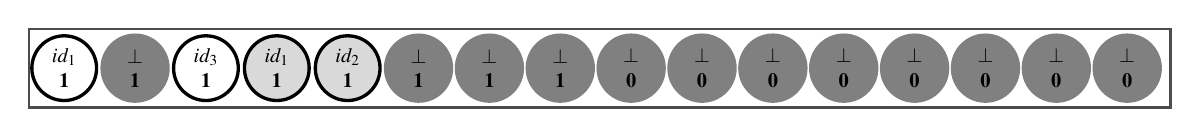
\begin{tikzpicture}
     [
     greenball/.style={circle, draw=black, align=center, fill=gray!30, very thick, minimum size=7mm},
     redball/.style={circle, draw=black,align=center, fill=white, very thick, minimum size=7mm},
     dummyball/.style={circle, draw=gray, align=center, fill=gray, very thick, minimum size=7mm},
     textbox/.style={rectangle, draw=white, fill=white, thick, minimum height=1cm},
     buffer1/.style={rectangle, draw=black!70, fill=white, thick, minimum height=1cm,minimum width=14.5cm},
     ]
  \node at (0,0) [buffer1] (buf) {};
 \node[scale=0.74] at (-6.8,0) [redball]   (ball1)  {$id_1$\\ \tblue{\textbf{1}}};
 \node[scale=0.74] at (-5.9,0) [dummyball]   (ball2)  {$~\bot~$\\ \tblue{\textbf{1}}};
 \node[scale=0.74] at (-5,0) [redball]   (ball3) {$id_3$\\ \tblue{\textbf{1}}};
 \node[scale=0.74] at (-4.1,0) [greenball]   (ball4) {$id_1$\\ \tblue{\textbf{1}}};
 \node[scale=0.74] at (-3.2,0) [greenball]   (ball5) {$id_2$\\ \tblue{\textbf{1}}};
 \node[scale=0.74] at (-2.3,0) [dummyball]   (d1)  {$~\bot~$\\ \tblue{\textbf{1}}};
 \node[scale=0.74] at (-1.4,0) [dummyball]   (d2)  {$~\bot~$\\ \tblue{\textbf{1}}};
 \node[scale=0.74] at (-0.5,0) [dummyball]   (d3)  {$~\bot~$\\ \tblue{\textbf{1}}};
 \node[scale=0.74] at (0.4,0) [dummyball]   (d4)  {$~\bot~$\\ \tred{\textbf{0}}};
 \node[scale=0.74] at (1.3,0) [dummyball]   (d5)  {$~\bot~$\\ \tred{\textbf{0}}};
 \node[scale=0.74] at (2.2,0) [dummyball]   (d6)  {$~\bot~$\\ \tred{\textbf{0}}};
 \node[scale=0.74] at (3.1,0) [dummyball] (rd7) {$~\bot~$\\ \tred{\textbf{0}}};    
 \node[scale=0.74] at (4,0) [dummyball] (d8) {$~\bot~$\\ \tred{\textbf{0}}};
 \node[scale=0.74] at (4.9,0) [dummyball] (d9) {$~\bot~$\\ \tred{\textbf{0}}};
 \node[scale=0.74] at (5.8,0) [dummyball] (d10)  {$~\bot~$\\ \tred{\textbf{0}}};
 \node[scale=0.74] at (6.7,0) [dummyball]  (d11) {$~\bot~$\\ \tred{\textbf{0}}};
   \end{tikzpicture}
   \captionsetup{justification=centering,font=large}
   \newsubcaption{$\BUF_1$ after the order preserving oblivious compaction in Phase 3}
 \label{fig:buf1g}
 \end{subfigure}
 }
 \end{figure*}


 \begin{figure*}[!h]
 \ContinuedFloat
 \centering
 %\scalebox{0.6}
 {
 \begin{subfigure}[]{0.8\textwidth}
 \centering
   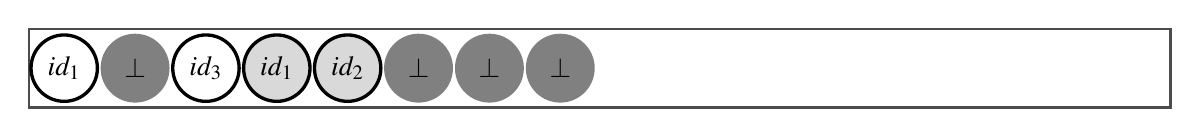
\begin{tikzpicture}
     [
     greenball/.style={circle, draw=black, align=center, fill=gray!30, very thick, minimum size=7mm},
     redball/.style={circle, draw=black,align=center, fill=white, very thick, minimum size=7mm},
     dummyball/.style={circle, draw=gray, align=center, fill=gray, very thick, minimum size=7mm},
     textbox/.style={rectangle, draw=white, fill=white, thick, minimum height=1cm},
     buffer1/.style={rectangle, draw=black!70, fill=white, thick, minimum height=1cm,minimum width=14.5cm},
     ]
  \node at (0,0) [buffer1] (buf) {};
 \node at (-6.8,0) [redball]   (ball1)  {$id_1$};
 \node[scale=1] at (-5.9,0) [dummyball]   (ball2)  {$~\bot~$};
 \node[scale=1] at (-5,0) [redball]   (ball3) {$id_3$};
 \node[scale=1] at (-4.1,0) [greenball]   (ball4) {$id_1$};
 \node[scale=1] at (-3.2,0) [greenball]   (ball5) {$id_2$};
 \node[scale=1] at (-2.3,0) [dummyball]   (d1)  {$~\bot~$};
 \node[scale=1] at (-1.4,0) [dummyball]   (d2)  {$~\bot~$};
 \node at (-0.5,0) [dummyball]   (d3)  {$~\bot~$};
 \end{tikzpicture}
   \captionsetup{justification=centering,font=large}
   \newsubcaption{$\BUF_1$ after discarding the 0/1-bit tags; at the end of Phase 3}
   \label{fig:buf1h}
 \end{subfigure}
 }
 \end{figure*}


%Every $b_i$ elements are randomly shuffled.


 \begin{figure*}[!h]
 \ContinuedFloat
 \centering
 %\scalebox{0.6}{
 \begin{subfigure}[]{0.5\textwidth}
 \centering
     \begin{tikzpicture}
 [
 greenball/.style={circle, draw=black, align=center, fill=gray!30, very thick, minimum size=7mm},
 redball/.style={circle, draw=black,align=center, fill=white, very thick, minimum size=7mm},
 blueball/.style={circle, draw=blue!40, fill=blue!40, very thick, minimum size=7mm},
 yellowball/.style={circle, draw=yellow!40, fill=yellow!40, very thick, minimum size=7mm},
 dummyball/.style={circle, draw=gray, fill=gray, very thick, minimum size=7mm},
 bin/.style={cylinder, draw=black!70, fill=white, thick, minimum height=2.4cm, minimum width = 1cm, rotate=90},
 textbox/.style={rectangle, draw=white, fill=white, thick, minimum height=1cm}
 ]
  \node at (1,0.5) [bin] (bin1) {};
 \node at (1,0) [redball]  (ball1)  {$id_1$};
 \node at (1,1) [dummyball]   (d1)  {$~\bot~$};
 \node at (2.3,0.5) [bin] (bin2) {};
 \node at (2.3,0) [greenball]   (d2)  {$id_1$};
 \node at (2.3,1) [redball]  (ball2) {$id_3$};
 \node at (3.6,0.5) [bin] (bin1) {};
 \node at (3.6,0) [dummyball]      (ball3)    {$~\bot~$};
 \node at (3.6,1) [greenball]      (d3)    {$id_2$};
 \node at (4.9,0.5) [bin] (bin2) {};
  \node at (4.9,0) [dummyball]      (ball4)  {$~\bot~$};
  \node at (4.9,1) [redball]      (ball5)    {$~\bot~$};
 \end{tikzpicture}
 \captionsetup{justification=centering,font=large}
 \newsubcaption{$\NEW_{i}.\Ind$ after random shuffle}
 \label{fig:buf1i}
 \end{subfigure}
 %}
 \caption{Different phases and steps of \omerge. Figure \ref{fig:buf1d} shows an an intermediate $\BUF_1$ state after a call to \omerge$_i$. The whole process takes a total of $2^i$ calls to \omerge$_i$. We have only shown the index part, and omitted the dictionary.}
 \label{fig:LSDdEx}
 \end{figure*}






\section{Performance of Amortized Schemes} \label{append:perf-amort}

In this section, we evaluate the performance of the amortized schemes and provide some experiments for their real-world use case. 

Figure~\ref{app-fig:update} shows an experiment that  measures the update time for 1K consecutive updates. In each update, the client fetches and merges some of the previously built levels and then uploads them to the server. 

Figure~\ref{app-fig:real} shows the search for different result sizes on two attributes of the crime dataset \cite{crimes}, each of which has (a) $34$, (b) $170$ distinct keywords. We measured the search time for different keywords associated with  the increasing number of results.

Figure~\ref{app-fig:search-var-amor-deamor} shows the search  time of different amortized schemes (including \LSDd[$sN$] for $s$ equal to 3 and 6) for a dataset with size $2^{23}$ when the result size varies between 10 and 5M.

Figure~\ref{app-fig:search-var} compares different amortized schemes in HDD (a,b,c,d) and SSD (e,f,g) for variable result sizes (a,b,e) and variable dataset sizes (c,d,f,g). All figures except Figure~\ref{app-fig:search-var}(b) which shows the result for block size 512, represent the experiment results for $|block|=32$.

\begin{figure}[!ht]
	\centering
	\begin{subfigure}[t]{0.48\linewidth}
		\includegraphics[width=\textwidth]{chapters/iodse/figures/Insert-SDA2.eps}
		\vspace{-0.6cm}
		\caption{}
	\end{subfigure}
 \begin{subfigure}[t]{0.48\linewidth}
		\includegraphics[width=\textwidth]{chapters/iodse/figures/Insert-SDA3.eps}
		\vspace{-0.6cm}
		\caption{}
	\end{subfigure}
	\vspace{-.3cm}
	\caption{Update computation time of amortized schemes for 1K updates starting from an empty dataset (a) \SDa[\OneChoice] vs \SDa[\PiBas] (b) \SDa[\NlogN] vs \SDa[\PiBas] }
	\label{app-fig:update}
% 	\vspace{-.3cm}
\end{figure}


\begin{figure}[!ht]
	\centering
	\begin{subfigure}[t]{0.48\linewidth}
		\includegraphics[width=\textwidth]{chapters/iodse/figures/Search-Crime1.eps}
		\vspace{-0.8cm}
		\caption{}
	\end{subfigure}
	\begin{subfigure}[t]{0.48\linewidth}
		\includegraphics[width=\textwidth]{chapters/iodse/figures/Search-Crime2.eps}
		\vspace{-.8cm}
		\caption{}
	\end{subfigure}%
	
	\vspace{-.3cm}
	\caption{Crime Dataset---Search computation time vs variable result size for an attributed with (a) $|W|=34$, (b) $|W|=170$.}
	\label{app-fig:real}
% 	\vspace{-.3cm}
\end{figure}





\begin{figure}[!ht]
	\centering
	\begin{subfigure}[t]{0.49\linewidth}
		\includegraphics[width=\textwidth]{chapters/iodse/figures/Search-SDA.eps}
		\vspace{-0.8cm}
		\caption{}
	\end{subfigure}
	\begin{subfigure}[t]{0.49\linewidth}
		\includegraphics[width=\textwidth]{chapters/iodse/figures/Search-SDA-SSD.eps}
		\vspace{-.8cm}
		\caption{}
	\end{subfigure}%
	\vspace{-.3cm}
	\caption{Search computation time for $|{DB}|=2^{23}$, variable result size, and $|block|=32$B for different \NlogN settings in (a) amortized HDD, (b) amortized SSD.}
	\label{app-fig:search-var-amor-deamor}
% 	\vspace{-.3cm}
\end{figure}


\begin{figure*}[ht]
	\centering
	\begin{subfigure}[t]{0.24\linewidth}
		\includegraphics[width=\textwidth]{chapters/iodse/figures/Search-Comp-DBSize10M-ResultSizeVar-32B-NoCache-2.eps}
		\vspace{-0.8cm}
		\caption{}
	\end{subfigure}
	\begin{subfigure}[t]{0.24\linewidth}
		\includegraphics[width=\textwidth]{chapters/iodse/figures/Search-Comp-DBSize10M-ResultSizeVar-512B-NoCache-2.eps}
		\vspace{-.8cm}
		\caption{}
	\end{subfigure}%
		\begin{subfigure}[t]{0.24\linewidth}
		\includegraphics[width=\textwidth]{chapters/iodse/figures/Search-Comp-DBSizeVar-ResultSize1000-2.eps}
		\vspace{-.8cm}
		\caption{}
	\end{subfigure}~
 	\begin{subfigure}[t]{0.24\linewidth}
		\includegraphics[width=\textwidth]{chapters/iodse/figures/Search-Comp-DBSizeVar-ResultSize10000-2.eps}
		\vspace{-.8cm}
		\caption{}
	\end{subfigure}~\\
% 	\vspace{-.4cm}
% 	\caption{Search computation time for $|{DB}|=2^{23}$ and variable result size for: (a) $|block|=32$B in HDD, (a) $|block|=32$B in SSD, (c) $|block|=512$B in HDD.}
% 	\label{fig:search-var-block}
	\vspace{-.2cm}
% \end{figure*}

% \begin{figure*}[ht]
% 	\centering
	\begin{subfigure}[t]{0.24\linewidth}
		\includegraphics[width=\textwidth]{chapters/iodse/figures/Search-Comp-DBSize10M-ResultSizeVar-32B-NoCache-SSD-2.eps}
		\vspace{-0.8cm}
		\caption{}
	\end{subfigure}
	\begin{subfigure}[t]{0.24\linewidth}
		\includegraphics[width=\textwidth]{chapters/iodse/figures/Search-Comp-DBSizeVar-ResultSize1000-SSD-2.eps}
		\vspace{-.8cm}
		\caption{}
	\end{subfigure}%
		\begin{subfigure}[t]{0.24\linewidth}
		\includegraphics[width=\textwidth]{chapters/iodse/figures/Search-Comp-DBSizeVar-ResultSize10000-SSD-2.eps}
		\vspace{-.8cm}
		\caption{}
	\end{subfigure}~
	\vspace{-.3cm}
	\caption{Search computation time for $|{DB}|=2^{23}$ and variable result size for (a) $|block|=32$B in HDD, (b) $|block|=512$B in HDD. Search computation time for variable database size and (c) $n_w=1K$ in HDD, (d) $n_w=10K$ in HDD. Search computation time for $|{DB}|=2^{23}$ and variable result size for (e) $|block|=32$B in SSD. Search computation time for variable database size and (f) $n_w=1K$ in SSD, (g) $n_w=10K$ in SSD.}
	\label{app-fig:search-var}
% 	\vspace{-.3cm}
\end{figure*}


\section{Performance of De-Amortized Schemes} \label{append:perf-deamort}

In this section, we provide some extra experiments for the de-amortized schemes. Figure~\ref{app-fig:search-var2} (a) shows the search time when the result size varies between 10 and 5M where the dataset size is $2^{23}$ and the block size is $512$ bytes. Figure~\ref{app-fig:search-var2} (b,c) show the search computation time where database size varies between $2^{14}-2^{26}$ for (b) HDD and (c) SSD. Finally, Figure~\ref{app-fig:search-var2} (d) shows the end-to-end search time over WAN where the machines are located in Ireland and Frankfurt with 24.7ms delay.

\begin{figure*}[ht]
	\centering
	\begin{subfigure}[t]{0.24\linewidth}
		\includegraphics[width=\textwidth]{chapters/iodse/figures/Cache-25-SSD.eps}
		\vspace{-.8cm}
		\caption{}
	\end{subfigure}%
		\begin{subfigure}[t]{0.24\linewidth}
		\includegraphics[width=\textwidth]{chapters/iodse/figures/Cache-50-SSD.eps}
		\vspace{-.8cm}
		\caption{}
	\end{subfigure}~
 	\begin{subfigure}[t]{0.24\linewidth}
		\includegraphics[width=\textwidth]{chapters/iodse/figures/Cache-75-SSD.eps}
		\vspace{-.8cm}
		\caption{}
	\end{subfigure}
    \begin{subfigure}[t]{0.24\linewidth}
		\includegraphics[width=\textwidth]{chapters/iodse/figures/Cache-100.eps}
		\vspace{-0.8cm}
		\caption{}
	\end{subfigure}~\\
	\vspace{-.4cm}
	\caption{Search computation time for $|{DB}|=2^{23}$ and variable result size for $|block|=32$B in SSD, (a) 25\% Caching, (b) 50\% Caching, (c) 75\% Caching, (d) 100\% Caching.}
	\label{fig:cache-ssd}
	\vspace{-.2cm}
\end{figure*}

\begin{figure}[ht]
	\centering
	\begin{subfigure}[t]{0.48\linewidth}
		\includegraphics[width=\textwidth]{chapters/iodse/figures/email-hdd.eps}
		\vspace{-0.6cm}
		\caption{}
	\end{subfigure}
 \begin{subfigure}[t]{0.48\linewidth}
		\includegraphics[width=\textwidth]{chapters/iodse/figures/email-ssd.eps}
		\vspace{-0.6cm}
		\caption{}
	\end{subfigure}
	\vspace{-.3cm}
	\caption{Search computation time for $|{DB}|=2^{20}$ for each user and variable result size for $|block|=32$B with caching enabled in (a) HDD where 200 users exist in the system (b) SSD where 75 users exist in the system}
	\label{fig:email}
% 	\vspace{-.3cm}
\end{figure}


\begin{figure}[ht]
	\centering
 \begin{subfigure}[t]{0.48\linewidth}
		\includegraphics[width=\textwidth]{chapters/iodse/figures/UpdateTime.eps}
		\vspace{-0.6cm}
		\caption{}
	\end{subfigure}
 \begin{subfigure}[t]{0.48\linewidth}
		\includegraphics[width=\textwidth]{chapters/iodse/figures/UpdateTime-WAN1.eps}
		\vspace{-0.6cm}
		\caption{}
	\end{subfigure}
	\vspace{-.3cm}	
	\caption{Update computation time for variable database sizes (a) over single machine (b) over WAN machines with 24.7ms network delay and 2.5Gbps bandwidth.}
	\label{fig:wan}
% 	\vspace{-.3cm}
\end{figure}



\begin{figure}
\small
 \centering\begin{tabular}{|c|c|c|} 
\hline
Scheme & Size(GB) for $|DB|=2^{23}$ & Size(GB) for $|DB|=2^{26}$ \\ 
\hline 
 \LSDd[\NlogN] & 49 & 436 \\
 \LSDd[\OneChoice] & 7.5 & 60\\
 \SDd[\PiBas] & 5 & 40 \\
\hline
\end{tabular}
%\end{adjustbox}
\caption{Needed storage for a dataset and encrypted index=$32B$}
\label{table:storage}
\end{figure} 

% \begin{figure}[ht]
% 	\centering

% 	\vspace{-.3cm}	
% 	\caption{Search computation time for $|{DB}|=2^{23}$, $|block|=32$B in HDD and variable result size for WAN machines with 24.7ms network delay and 2.5Gbps bandwidth.}
% 	\label{fig:app-wan}
% % 	\vspace{-.3cm}
% \end{figure}


\begin{figure*}[ht]
	\centering
	\begin{subfigure}[t]{0.24\linewidth}
		\includegraphics[width=\textwidth]{chapters/iodse/figures/Search-Comp-DBSize10M-ResultSizeVar-512B-NoCache.eps}
		\vspace{-.8cm}
		\caption{}
	\end{subfigure}%
 	\begin{subfigure}[t]{0.24\linewidth}
		\includegraphics[width=\textwidth]{chapters/iodse/figures/Search-Comp-DBSizeVar-ResultSize10000.eps}
		\vspace{-.8cm}
		\caption{}
	\end{subfigure}~
		\begin{subfigure}[t]{0.24\linewidth}
		\includegraphics[width=\textwidth]{chapters/iodse/figures/Search-Comp-DBSizeVar-ResultSize10000-SSD.eps}
		\vspace{-.8cm}
		\caption{}
	\end{subfigure}~
  \begin{subfigure}[t]{0.24\linewidth}
		\includegraphics[width=\textwidth]{chapters/iodse/figures/SearchTime-WAN2.eps}
		\vspace{-0.6cm}
	\end{subfigure}\\
	\vspace{-.3cm}
	\caption{Search computation time for $|{DB}|=2^{23}$ and variable result size for (a)  $|block|=512$B in HDD. Search computation time for variable database size and $n_w=10K$ in (b) HDD, (c) SSD. (d) Search computation time for $|{DB}|=2^{23}$, $|block|=32$B in HDD and variable result size for WAN machines with 24.7ms network delay and 2.5Gbps bandwidth..}
	\label{app-fig:search-var2}
% 	\vspace{-.3cm}
\end{figure*}



% \begin{figure*}[ht]
% 	\centering
% 	\begin{subfigure}[t]{0.24\linewidth}
% 		\includegraphics[width=\textwidth]{figures/Search-SDA.eps}
% 		\vspace{-0.8cm}
% 		\caption{}
% 	\end{subfigure}
% 	\begin{subfigure}[t]{0.24\linewidth}
% 		\includegraphics[width=\textwidth]{figures/Search-SDA-SSD.eps}
% 		\vspace{-.8cm}
% 		\caption{}
% 	\end{subfigure}%
% 		\begin{subfigure}[t]{0.24\linewidth}
% 		\includegraphics[width=\textwidth]{figures/Search-SDD.eps}
% 		\vspace{-.8cm}
% 		\caption{}
% 	\end{subfigure}~
% 	\begin{subfigure}[t]{0.24\linewidth}
% 		\includegraphics[width=\textwidth]{figures/Search-SDD-SSD.eps}
% 		\vspace{-.8cm}
% 		\caption{}
% 	\end{subfigure}%
% 	\vspace{-.3cm}
% 	\caption{Search computation time for $|{DB}|=2^{23}$, variable result size, and $|block|=32$B for different \NlogN settings in (a) amortized HDD, (b) amortized SSD, (c) de-amortized HDD, (d) de-Amortized SSD.}
% 	\label{fig:search-var-amor-deamor}
% % 	\vspace{-.3cm}
% \end{figure*}




% \begin{figure}[ht]
% 	\centering
%  \begin{subfigure}[t]{0.48\linewidth}
% 		\includegraphics[width=\textwidth]{figures/Cache-100.eps}
% 		\vspace{-0.6cm}
% 		\caption{}
% 	\end{subfigure}
%  \begin{subfigure}[t]{0.48\linewidth}
% 		\includegraphics[width=\textwidth]{figures/Cache-100-Server.eps}
% 		\vspace{-0.6cm}
% 		\caption{}
% 	\end{subfigure}
% 	\vspace{-.3cm}	
% 	\caption{(a) Search computation time for $|{DB}|=2^{23}$ and variable result size for $|block|=32$B in 100\% Caching (a) the whole search time (b) server time}
% 	\label{fig:cache2}
% % 	\vspace{-.3cm}
% \end{figure}





\begin{figure*}
\centering
\subfloat[1C]
{
\scalebox{0.8}
{
\begin{tikzpicture}
[
greenball/.style={circle, draw=gray, fill=gray,  thick, minimum size=7mm},
redball/.style={circle, draw=gray, fill=white,  thick, minimum size=7mm},
blueball/.style={circle, draw=black, fill=black,  thick, minimum size=7mm},
whiteball/.style={circle, draw=white, fill=white, very thick, minimum size=7mm},
dummyball/.style={circle, draw=gray, fill=gray, very thick, minimum size=7mm},
bin/.style={cylinder, draw=black!70, fill=white, thick, minimum height=2.4cm, minimum width = 1cm, rotate=90},
textbox/.style={rectangle, draw=white, fill=white, thick, minimum height=1cm},
myarrow1/.style={single arrow, draw=blue, fill=green, 
      minimum width = 10pt, single arrow head extend=3pt,
      minimum height=10mm}
]
\node at (2.3,-1) [textbox]      (tb1)    {Index};
 \node at (1,0.5) [bin] (bin1) {};
\node at (1,0) [greenball]      (ball1)    {};
\node at (1,1) [blueball]      (d1)     {};
 \node at (2.3,0.5) [bin] (bin2) {};
 \node at (2.3,0) [blueball]      (d2)    {};
 \node at (2.3,1) [redball]      (ball2)    {};
 \node at (3.6,0.5) [bin] (bin2) {};
 \node at (3.6,0) [blueball]      (d2)    {};
 \node at (3.6,1) [redball]      (ball2)      {};
 
 \draw[] (4.7,1.2) rectangle (6,-0.4) {};
 \node at (5.4,-1) [textbox]      (d1)       {Dictionary};
 \node[scale=0.6] at (5,0.9) [blueball]   (d1)  {};
 \node[scale=0.7] at (5.7,0.9) [whiteball]   (d1)  {3};
 
  \node[scale=0.6] at (5,0.4) [greenball]   (d1)  {};
  \node[scale=0.7] at (5.7,0.4) [whiteball]   (d1)  {1};
  
   \node[scale=0.6] at (5,-0.1) [redball]   (d1)  {};
   \node[scale=0.7] at (5.7,-0.1) [whiteball]   (d1)  {2};
   \draw[] (4.7,0.65) -- (6,0.65) ;
    \draw[] (4.7,0.15) -- (6,0.15) ;
    \draw[thick,dashed] (5.4,1.2) -- (5.4,-0.4) {};
\end{tikzpicture}
}
}
%\hspace*{\fill}
\hspace*{20pt}
\subfloat[NlogN]
{
\scalebox{0.8}{
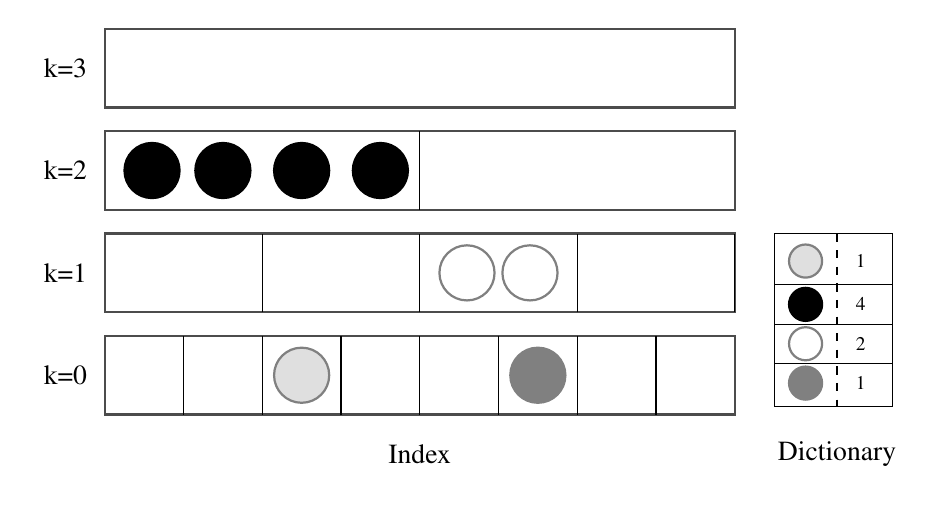
\begin{tikzpicture}
[
grayball/.style={circle, draw=gray, fill=gray,  thick, minimum size=7mm},
lightgrayball/.style={circle, draw=gray, fill=gray!25,  thick, minimum size=7mm},
gwball/.style={circle, draw=gray, fill=white,  thick, minimum size=7mm},
blackball/.style={circle, draw=black, fill=black,  thick, minimum size=7mm},
whiteball/.style={circle, draw=white, fill=white, very thick, minimum size=7mm},
dummyball/.style={circle, draw=gray, fill=gray, very thick, minimum size=7mm},
bin/.style={rectangle, draw=black!70, fill=white, thick, minimum height=8cm, minimum width = 1cm, rotate=90},
textbox/.style={rectangle, draw=white, fill=white, thick, minimum height=1cm},
myarrow1/.style={single arrow, draw=blue, fill=green, 
      minimum width = 10pt, single arrow head extend=3pt,
      minimum height=10mm}
]
\node at (0,-1) [textbox]      (tb1)    {Index};
%level 0
\node at (-4.5,0) [whiteball] (w1) {k=0};
\node at (0,0) [bin] (bin1) {};
\draw[] (-3,-0.5) -- (-3,0.5) ;
\draw[] (-2,-0.5) -- (-2,0.5) ;
\draw[] (-1,-0.5) -- (-1,0.5) ;
\node at (-1.5, 0) [lightgrayball] (lgb) {};
\draw[] (0,-0.5) -- (0,0.5) ;
\draw[] (1,-0.5) -- (1,0.5) ;
\draw[] (2,-0.5) -- (2,0.5) ;
\node at (1.5, 0) [grayball] (gb) {};
\draw[] (3,-0.5) -- (3,0.5) ;

 %level 1
 \node at (-4.5,1.3) [whiteball] (w1) {k=1};
\node at (0, 1.3) [bin] (bin2) {};
\draw[] (-2,0.8) -- (-2,1.8) ;
\draw[] (0,0.8) -- (0,1.8) ;
\draw[] (2,0.8) -- (2,1.8) ;
\node at (0.6,1.3) [gwball] (wb1) {};
\node at (1.4,1.3) [gwball] (wb2) {};
\draw[] (4,0.8) -- (4,1.8) ;

%level 2
\node at (-4.5,2.6) [whiteball] (w1) {k=2};
\node at (0, 2.6) [bin] (bin3) {};
\draw[] (0,2.1) -- (0,3.1) ;
\node at (-3.4,2.6) [blackball] (bb1) {};
\node at (-2.5,2.6) [blackball] (bb1) {};
\node at (-1.5,2.6) [blackball] (bb1) {};
\node at (-0.5,2.6) [blackball] (bb1) {};
%level 3
\node at (-4.5,3.9) [whiteball] (w1) {k=3};
\node at (0, 3.9) [bin] (bin4) {};

 %%dictionary

 \draw[] (4.5,1.8) rectangle (6,-0.4) {};
 \node at (5.3,-1) [textbox]      (d1)       {Dictionary};
 \node[scale=0.6] at (4.9,0.9) [blackball]   (d1)  {};
 \node[scale=0.7] at (5.6,0.9) [whiteball]   (d1)  {4};
 
  \node[scale=0.6] at (4.9,0.4) [gwball]   (d1)  {};
  \node[scale=0.7] at (5.6,0.4) [whiteball]   (d1)  {2};
  
   \node[scale=0.6] at (4.9,-0.1) [grayball]   (d1)  {};
   \node[scale=0.7] at (5.6,-0.1) [whiteball]   (d1)  {1};
   \node[scale=0.6] at (4.9,1.45) [lightgrayball]   (d1)  {};
   \node[scale=0.7] at (5.6,1.45) [whiteball]   (d1)  {1};
   \draw[] (4.5,0.65) -- (6,0.65) ;
   \draw[] (4.5,0.15) -- (6,0.15) ;
   \draw[] (4.5,1.15) -- (6,1.15);
   \draw[thick,dashed] (5.3,1.8) -- (5.3,-0.4) {};

\end{tikzpicture}
}
}


\vspace{0.7cm}
\subfloat[2C (Part I). Braces indicate superbin.]
{
\scalebox{0.8}
{
\begin{tikzpicture}
[
grayball/.style={circle, draw=gray, fill=gray,  thick, minimum size=7mm},
lightgrayball/.style={circle, draw=gray, fill=gray!25,  thick, minimum size=7mm},
gwball/.style={circle, draw=gray, fill=white,  thick, minimum size=7mm},
blackball/.style={circle, draw=black, fill=black,  thick, minimum size=7mm},
whiteball/.style={circle, draw=white, fill=white, very thick, minimum size=7mm},
dummyball/.style={circle, draw=gray, fill=gray, very thick, minimum size=7mm},
bin/.style={cylinder, draw=black!70, fill=white, thick, minimum height=3cm, minimum width = 1cm, rotate=90},
textbox/.style={rectangle, draw=white, fill=white, thick, minimum height=1cm},
myarrow1/.style={single arrow, draw=blue, fill=green, 
      minimum width = 10pt, single arrow head extend=3pt,
      minimum height=10mm}
]
\node at (3,-1.2) [textbox]      (tb1)    {Index};
\draw [decorate, decoration = {brace, amplitude = 10pt}, dashed, thick] (0.5,2.8) --  (5.4,2.8);
\draw [decorate, decoration = {brace, amplitude = 7pt}] (0.5,2.3) --  (2.7,2.3);
 \node at (1,0.5) [bin] (bin1) {};
\node at (1,-0.4) [blackball]      (ball1)    {};
\node at (1,0.5) [gwball]      (d1)     {};
\node at (2.3,1.5) [gwball]      (d1)     {};

 \node at (2.3,0.5) [bin] (bin2) {};
 \node at (2.3,-0.4) [blackball]      (d2)    {};
 \node at (2.3,0.5) [gwball]      (d1)     {};
 
\draw [decorate, decoration = {brace, amplitude = 7pt}] (3.2,2.3) --  (5.4,2.3);
 \node at (3.6,0.5) [bin] (bin3) {};
 \node at (3.6,-0.4) [blackball]      (d2)    {};
% \node at (3.6,0.5) [gwball]      (ball2)      {};
 
 \node at (4.9, 0.5) [bin] (bin4) {};
 \node at (4.9,-0.4) [blackball]      (d2)    {};
 %\node at (4.9,0.5) [gwball]      (ball2)    {};

 %%dictionary
 \draw[] (6,1.8) rectangle (7.5,-0.4) {};
 \node at (6.8,-1) [textbox]      (d1)       {Dictionary};
 \node[scale=0.6] at (6.4,0.9) [blackball]   (d1)  {};
 \node[scale=0.7] at (7.1,0.9) [whiteball]   (d1)  {4};
 
  \node[scale=0.6] at (6.4,0.4) [gwball]   (d1)  {};
  \node[scale=0.7] at (7.1,0.4) [whiteball]   (d1)  {2};
  
   %\node[scale=0.6] at (6.4,-0.1) [grayball]   (d1)  {};
   %\node[scale=0.7] at (7.1,-0.1) [whiteball]   (d1)  {1};
  % \node[scale=0.6] at (6.4,1.45) [lightgrayball]   (d1)  {};
   %\node[scale=0.7] at (7.1,1.45) [whiteball]   (d1)  {1};
   \draw[] (6,0.65) -- (7.5,0.65) ;
    \draw[] (6,0.15) -- (7.5,0.15) ;
    \draw[] (6,1.15) -- (7.5,1.15);
    \draw[thick,dashed] (6.8,1.8) -- (6.8,-0.4) {};

 \end{tikzpicture}
}
}
\hspace*{90pt}
\subfloat[2C (Part II)]
{
\scalebox{0.8}{
\begin{tikzpicture}
[
grayball/.style={circle, draw=gray, fill=gray,  thick, minimum size=7mm},
lightgrayball/.style={circle, draw=gray, fill=gray!25,  thick, minimum size=7mm},
gwball/.style={circle, draw=gray, fill=white,  thick, minimum size=7mm},
blackball/.style={circle, draw=black, fill=black,  thick, minimum size=7mm},
whiteball/.style={circle, draw=white, fill=white, very thick, minimum size=7mm},
dummyball/.style={circle, draw=gray, fill=gray, very thick, minimum size=7mm},
bin/.style={cylinder, draw=black!70, fill=white, thick, minimum height=3cm, minimum width = 1cm, rotate=90},
textbox/.style={rectangle, draw=white, fill=white, thick, minimum height=1cm},
myarrow1/.style={single arrow, draw=blue, fill=green, 
      minimum width = 10pt, single arrow head extend=3pt,
      minimum height=10mm}
]
\node at (3,-1.2) [textbox]      (tb1)    {Index};
\node at (1,0.5) [bin] (bin1) {};
\draw [decorate, decoration = {brace, amplitude = 7pt}, very thick] (0.5,2.7) --  (1.5,2.7);
\draw [decorate, decoration = {brace, amplitude = 7pt}] (0.5,2.3) --  (1.5,2.3);
\node at (1,-0.4) [blackball]      (ball1)    {};
\node at (1,0.5) [gwball]      (d1)     {};


 \node at (2.3,0.5) [bin] (bin2) {};
 \node at (2.3,-0.4) [blackball]      (d2)    {};
 \node at (2.3,0.5) [gwball]      (d1)     {};

 \draw [decorate, decoration = {brace, amplitude = 7pt}, very thick] (3.1,2.7) --  (4.1,2.7);
 \node at (3.6,0.5) [bin] (bin3) {};
 \node at (3.6,-0.4) [blackball]      (d2)    {};
 \node at (3.6,0.5) [lightgrayball]      (ball2)      {};

 \draw [decorate, decoration = {brace, amplitude = 7pt}] (4.4,2.3) --  (5.4,2.3);
 \node at (4.9, 0.5) [bin] (bin4) {};
 \node at (4.9,-0.4) [blackball]      (d2)    {};
 \node at (4.9,0.5) [grayball]      (d1)     {};
 %\node at (4.9,1) [gwball]      (ball2)    {};

 %%dictionary
 
 \draw[] (6,1.8) rectangle (7.5,-0.4) {};
 \node at (6.8,-1) [textbox]      (d1)       {Dictionary};
 \node[scale=0.6] at (6.4,0.9) [blackball]   (d1)  {};
 \node[scale=0.7] at (7.1,0.9) [whiteball]   (d1)  {4};
 
  \node[scale=0.6] at (6.4,0.4) [gwball]   (d1)  {};
  \node[scale=0.7] at (7.1,0.4) [whiteball]   (d1)  {2};
  
   \node[scale=0.6] at (6.4,-0.1) [grayball]   (d1)  {};
   \node[scale=0.7] at (7.1,-0.1) [whiteball]   (d1)  {1};
   \node[scale=0.6] at (6.4,1.45) [lightgrayball]   (d1)  {};
   \node[scale=0.7] at (7.1,1.45) [whiteball]   (d1)  {1};
   \draw[] (6,0.65) -- (7.5,0.65) ;
    \draw[] (6,0.15) -- (7.5,0.15) ;
    \draw[] (6,1.15) -- (7.5,1.15);
    \draw[thick,dashed] (6.8,1.8) -- (6.8,-0.4) {};

\end{tikzpicture}
}
}
\caption{Each keyword is visualized with a color and an entry in the index of that keyword is visualized as ball of that particular color. In \OneChoice\ and \TwoChoice\, after assigning the entries to the bins, the bins are filled with dummy entries and each bin is randomly shuffled. The length of the input dataset is $N$. For \TwoChoice\ and \NlogN\ schemes each keyword list is padded to be power 2. A dictionary is maintained in each of these schemes. \textbf{(a)} In \OneChoice\ scheme $m=N/\log N \log \log N$ bins are allocated, each of size $3\log N \log \log N$. Same colored balls are stored in adjacent bins. The first bin is calculated with a hash function $h(\bullet)$. The $k$th ball is stored at bin $(h(\bullet)+k)\%m$. For example, for the black ball $h(\bullet)$ returns 1. Hence, the first ball (k=0) is stored in bin $(h(\bullet)+0)\%3)=1$, the second ball (k=1) in bin $(h(\bullet)+1)\%3)=2$, and the third ball (k=2) is stored (wraps-around) in bin$(h(\bullet)+2)\%3)=0$. \textbf{(b)} The \NlogN\ scheme instantiates $(\log N +1)$ levels each of size $N$. The $k$th level stores lists of size $2^k$, in a contiguous memory chunk; i.e. each level is divided into $N/2^k$ chunks. We have 8 elements, hence we have $(\log 8 +1)=4$ levels. Because the list of black balls is of size 4, it is stored in level 2 (as $2^2 = 4$). Similarly, the list of white balls is stored in level 1. The gray and the light gray lists consist of single element each, and hence they get stored in level 0. A hash function is used to decide which memory chunk stores the data. 
\textbf{(c)} \TwoChoice\ allocates  $m={N}/{(\log\log N)^A (\log \log \log N)^2}$ bins, of size $z{\cdot}(\log\log N)^A$ ($\log$$\log$$\log N)^2$, ($2\leq z \leq 4$ , we use $A=1$).
Keyword lists are stored in \emph{decreasing order} of their lengths; e.g. the list of black balls will be stored first, and then the list of white balls and so on. For each keyword $w$, first
it divides the bins into groups of $sb = \frac{m}{n_w}$ \emph{superbins}; e.g. for the list of black balls we have $4/4 =1$ superbin consisting of 4 bins (marked with a dashed curly brace), while for the list of white balls, we have $4/2 =2$ superbins, consisting of 2 bins each (marked with two separate curly braces). Then two prospective superbins for a particular keyword are computed using two hash values $h_1(\bullet)\% sb$ and $h_2(\bullet)\%sb$; and superbin with minimal load is chosen. Both the superbins for the white balls have same load, so anyone can be chosen. \textbf{(d)} The two superbins for the gray ball is computed to be bin $0$ and bin $2$. Bin $2$ has one black ball, while bin $0$ has one black and a white ball, hence the superbin with minimal load is bin $2$. Similarly, for the light gray ball, whose superbins are bin $0$ and bin $3$, is stored in bin $3$. The 
corresponding hash functions and the dictionary is used during a search operation.}
\label{fig:allSEschemes}
\end{figure*}



%\section{DSE Security}\label{app:sse}
\mdfdefinestyle{mystyle2}{userdefinedwidth=20cm,rightmargin=0.7cm}
\begin{figure*}[!h]
\begin{mdframed}[style=mystyle2]
$EDB$ consists of two parts; 
$EDB.\Ind$ stores the encrypted \OneChoice~ array and
$EDB.\Dict$ stores an encrypted dictionary \\
Let $\RND = (\Enc, \Dec, \keyGen)$ is CPA-secure encryption scheme \\
\vspace{-1cm}
\begin{multicols}{2}
 \underline{$(K,\sigma;EDB) \leftarrow \texttt{Setup}(1^\lambda,DB)$}
 \begin{algorithmic}[1]
  \State $F:\{0,1\}^{*}\times \{0,1\}^{\lambda} \xrightarrow[]{} \{0,1\}^{*}$ is a PRF
  \State $(k_{rnd},k_{prf}) \gets {\texttt{KeyGen}}(1^\lambda)$ 
   \State $N \gets |DB|$
  \State $binSize \gets max(3\cdot \log N \log \log N,1)$ 
  \State $maxBins \gets max(\ceil{\frac{N}{\log N \log \log N}},1)$ 
  \State Initialize empty map \textbf{M} of size $N$
%  \State Fill up array $\BUF$ of size $3{\cdot} N $ with $\RND.\Enc(k_{rnd},(\dummy, \dummy,\dummy))$
%  \Statex{\tpurp{$\rhd$ The third attribute is the extra piece }}
 % \Statex{\tpurp{of data that is needed per entry in our DSE constructions}}
  %\State Initialize an empty Map $L$ that maps each unique keyword of $DB$ to the list of entries for that keyword in $DB$ 
  %\State For each unique keyword $w$ add all entries $(w,id,op)\in DB$ to $L$
  %  by calling $L[w].\Append((w,id,op))$
   \State Create separate lists with entries of each unique keyword $L=\{l_{w_1},l_{w_2}, \ldots, l_{w_n}\}$
\For{$i=1 \ldots n$}
\State $cnt \gets 0$
  \For{each entry $(w_i,id.op) \in l_{w_i}$}
  \State  $((bin,pos),\sigma) \gets \texttt{Map}(k_{prf},w_i,cnt,|l_{w_i}|,N,\sigma)$
 \State Place $\RND.\Enc(k_{rnd},(w_i,id,op))$ in the next available spot in $bin$ in $\BUF$
 \State $cnt \gets cnt+1$
   %\State Parse $l$ as $(w,l')$, and $l'$ as $\{e_1,e_2,\ldots, e_n \}$
   %\State $start \gets ((h(w)+cnt_w)\%m)\cdot binSize $
% \State $((bin,0),\sigma) \gets \texttt{Map}(k_{prf},w,1,|DB(w)|,N,\sigma)$
 \EndFor
    \State  \textbf{M}$[H(F(k_{prf},w_i),1)] \gets \RND.\textsf{Enc}(k_{rnd},|l_{w_i}|)$
   \EndFor
   \State Pad every bin to maximum capacity with $\RND.\Enc(k_{rnd},(\dummy, \dummy,\dummy))$ and randomly shuffle each bin
   \State $EDB.\Ind \gets \BUF$ and $EDB.\Dict \gets $ \textbf{M}
   \State Store $K$ as $(k_{rnd},k_{prf})$ and $maxBins$ and $binSize$ in $\sigma$ 
   \State \Return $EDB$ to server
   \Statex
   \Statex
    \end{algorithmic}
    

\underline{$(k_{rnd},k_{prf}) \leftarrow \texttt{KeyGen}(1^\lambda)$}
\begin{algorithmic}[1]
 \State $k_{prf} \gets $Choose a random PRF key for $F$
 \State Set $k_{rnd} \leftarrow$ \RND.\keyGen$(1^\lambda)$ 
  %\State $k_{prf_{cnt}} \gets $Choose a random PRF key for $F$
 %\State Randomly choose hash function $h$ from family $\mathcal{H}$
 \State \Return $(k_{rnd},k_{prf})$
\end{algorithmic}

% \underline{$bin \leftarrow \texttt{Map}(w,cnt_w,m,h)$}
 \underline{$((binNum,pos),\sigma) \leftarrow \texttt{Map}(k_{prf}, w, rank,n_w,\sigma)$}
\begin{algorithmic}[1]
%\State $maxBins \gets \ceil{\frac{N}{\log N \log \log N}}$
\If {$w \neq \dummy $}
 \State{ $binNum \gets (H(F(k_{prf},w),0)+rank)\%maxBins $}
 \Else 
 \State{ $binNum \gets \bot$}
 \EndIf
 \State {\Return $((binNum,0),\sigma)$}
\end{algorithmic}

%  \underline{$binNum \leftarrow \texttt{Map}(k_{prf}, w, cnt_w, maxBins)$}
%\begin{algorithmic}[1]
%\If {$w \neq \dummy $}
%\State{ $binNum \gets (H(F(k_{prf},w),0)+cnt_w)\%maxBins $}
 %\EndIf
 %\ElsI { $binNum \gets (maxBins)+1$}
 %\EndIIf
% \State {\Return $(binNum,0)$}
%\end{algorithmic}

\underline{$res \leftrightarrow \texttt{Search}(k,w,\sigma;EDB)$}
  \begin{algorithmic}[1]
  \item[Client $\leftrightarrow$ Server:]
  \State parse $k$ as $(k_{rnd},k_{prf})$
 % \State $bins \gets \ceil{\frac{N}{\log N \log \log N}}$;\quad $binSize \gets 3{\cdot}\log N \log \log N$
  \State $ n_w \gets \RND.\Dec(k_{rnd}, EDB.\Dict[H(F(k_{prf},w),1)])$
  %	\item[Client:]
  \State Client runs $((st,pos),\sigma) \gets\texttt{Map}(k_{prf},w,0,n_w,\sigma){\cdot} binSize$
%  \State Client runs $end \gets (start+cnt_w)\cdot binSize -1$
 % \item[Client $\leftrightarrow$ Server:]
  \State Client gets $eres \leftarrow$ $EDB.\Ind$[$st,\ldots,((st+n_w){\cdot} binSize)$]
%   \item[Client:]
   \State Client Initializes empty set $res$ to store results
   \For {each $e \in eres$}
    \State $(w',id, op) \gets \RND.\Dec(k_{rnd},e)$
    \IIf{$w' = w$}
    {$res \gets res \cup \{(w,id,op)\}$}
   \EndFor
 \State \Return $res$
  %\EndFor
\end{algorithmic}
\end{multicols}
\vspace{-0.5cm}
\underline {{${\sf NEW}_i$ $ \leftrightarrow$ {\OneChoice.\omerge$(K, \sigma, {\sf OLDEST}_{i - 1},{\sf OLDER}_{i - 1})$}}}
\begin{algorithmic}[1]
\item[Client $\leftrightarrow$ Server:]
\Statex \textcolor{blue}{//** \ \ Phase 1---Preparing sorted input array\ \   **//}	
\State Parse $K$ as $(k_{rnd},P)$;\quad $oldw \gets \bot$ ;\quad  $cnt \gets \bot$ \label{sdd1c:counter} %\Comment{all encryptions and decryptions are done with key $k_{rnd}$, $P$ is an array of PRF keys}
%\State Client initializes a tuple called $\pr$ as $(\bot, 0)$ and stores it in local state $\sigma$
\State Initialize arrays \BUF$_1$ of size $2{\cdot}3{\cdot}2^1$, and \BUF$_2$ of size $3{\cdot}2^i$ to be empty
\State Copy $\OLDEST_{i-1}.\Ind \cup \OLDER_{i-1}.\Ind$ to $\BUF_1$; obliviously sort $\BUF_1$ w.r.t. 
 lexicographic order of keywords
%\State Perform two linear scans (one in reverse and one in correct order) on $\BUF_1$, to add the $rank$ values to each entry of keyword $w$. The entries now look like $((w,id,op),rank)$, where $0 \leq rank < |DB(w)|$. 
%\State Perform two linear scans (one in reverse and one in correct order) on $\BUF_1$, to add the $rank$ and $n_w$ values to each entry of keyword $w$. The entries now look like $((w,id,op),rank,n_w)$, where $0 \leq rank < n_w$. 
%\State {Linear scan $\BUF_1$ and pad appropriately to make each list's size nearest power of 2, without leaking the actual list length}
   % \State {$cnt \gets 0$}
   %\State {Perform oblivious sort on $\BUF_1$ based on lexicographic order of the keywords and  descending order of the $n_w$ values. Keep first $\Sigma.N$ elements.}
   % 
  \Statex \textcolor{blue}{//** \ \ Phase 2---Move elements and Prepare keyword counters \ \ **//}	
    \For{each $j = 1 \ldots |\BUF_1|$} %\tpurp{optimize with pair}
%    \State $((w,id,op),rank,n_w) \gets \RND.\Dec(k_{rnd},\BUF_1[j])$ %and parse $\pr$ as $(w',cnt)$
     \State $(w,id,op) \gets \RND.\Dec(k_{rnd},\BUF_1[j])$; \quad {$p \gets^{\$} \{0,1\}^\lambda$}
      \If{~~$(w$ is observed for first time $\wedge$ $oldw \neq \bot)$}    \State {$\BUF_{2}.\Append(\RND.\Enc(k_{rnd},(oldw,cnt,p)))$;\quad $oldw \gets w$ ; \quad $cnt \gets 0$} 
      \label{sdd1c:resetCounter}
      \EndIf
      \ElsI{~~$\BUF_{2}.\Append(\RND.\Enc(k_{rnd},(\bot,\bot,\bot)))$; \quad $cnt\plus\plus$}
      %\EndIf
    %\If{$w' \neq w$ and $w' \neq \bot$} \Comment{i.e. Client is seeing $w$ for the first time}
    %\IIf{$rank = 0$}{~$\BUF_{2}.\Append(\RND.\Enc(k_{rnd},((w,n_w),p)))$}%; \quad {$cnt \gets 1$}
    %\ElsI{$\BUF_{2}.\Append(\RND.\Enc(k_{rnd},((\bot,0),0)))$}%; \quad {$cnt \textsc{++}$}
    %\EndIf
    %\State Client stores $(w,cnt)$ as $\pr$ in local state $\sigma$
   % \State $\pr \gets (w,cnt)$ \Comment{$\pr$ is updated with latest keyword and counter}
    \State $((bin,pos),\sigma)\gets\OneChoice.\texttt{Map}(P[i][3],w,cnt,\bot,\sigma)$ \label{sdd1c:map}%\Comment{$m_i$ = number of bins for \OneChoice~ for $2^i$ elements}
  \State \BUF$_{1}.\Append(\RND.\Enc(k_{rnd},(w,id,op,bin,pos)))$ \Comment{bin tag is added per entry}
    \EndFor
%    \State Parse $\pr$ as $(w',cnt')$ \Comment{for the last keyword in \textsf{SORTED}}
 %   \If{$w' \neq \bot$} 
 %   \State {$ p \gets^{\$} \{0,1\}^\lambda$ 
  %  \State $\BUF_{2}.\Append(\RND.\Enc(k_{rnd},((w',cnt'),p))$}
% \Else
%    \State {$\BUF_{2}.\Append(\RND.\Enc(k_{rnd},((\bot,0),0))$}
 %   \EndIf
    \Statex \textcolor{blue}{//** \ \ Phase 3---Add dummies\ \ **//}	\Comment{this phase adds binsize dummy entries per bin}
    \For{$bin= 0 \ldots \ceil{\frac{2^i}{\log 2^i \log \log 2^i}}-1$}
    \State Append $\RND.\Enc(k_{rnd},(\bot,\bot,\bot,bin,0))$ to $\BUF_1$  $3{\cdot} \log 2^i\log \log 2^i$ times \Comment{size of bins in \OneChoice~ when $N=2^i$}
    \EndFor
     \Statex \textcolor{blue}{//** \ \ Phase 4---Final placement \ \ **//}	
    \State Perform oblivious sort on $\BUF_1$ w.r.t. the $bin$ values of $(bin,0)$ pair in ascending order%; discard the bin tags
    \State Linearly scan $\BUF_1$, and tag \textbf{first} $3{\cdot} \log 2^i\log \log 2^i$ entries for each $bin\in \{0, \ldots, \ceil{\frac{2^i}{\log 2^i \log 2^i \log 2^i}}\}$ with 1, and with 0 the rest of them (existing $(bin,0)$ tags are replaced with 0/1 tags, entries now look like $(w,id,op,x)$, where $x \in \{0,1\}$)
        \State {Perform order preserving oblivious compaction on $\BUF_1$; keep first $\Sigma.N$ entries; discard the 0/1 tags }
    \State Perform oblivious sort on $\BUF_2$ w.r.t. the random keys in ascending order; keep first $2^i$ entries; discard random keys
    \State 	\NEW$_i.\OneChoice$ $\gets$ \BUF$_1$ and randomly shuffle each bin
   \For{each $s \in \BUF_2$}
\State $(w, cnt_w) \gets \RND.\Dec(k_{rnd}, s)$
\State $(key,value) \gets \PiBas.\MAP((P[i][3],k_{rnd}),w,cnt_w,1)$ \Comment{parameter 1 is used by the PRF $F$}
%\State $key \gets H(F(P[i][3],w),1)$ and $value \gets \RND.\Enc(R[i][3],cnt_w)$
\State 	\NEW$_i.$\Dict[$key$] $\gets value$
\EndFor
\State \Return \NEW$_i$
%\Statex (keep $3.2^i$ size of dictionary and explain we can optimize to $2^i$ size with extra 5-6 lines, write a paragraph about it, but if you can do it in the pseudocode do it)
%\Statex \tpurp{Client storage is logN because there are logN indexes}
\end{algorithmic}

\end{mdframed}
%\vspace{-.3cm}
\caption{One-Choice Allocation (\OneChoice.\omerge\ is the optimized version)}
\label{alg:1C} \label{alg:sdd1C}
\end{figure*}






\begin{figure*}[!h]
\begin{mdframed}
$EDB$ consists of two parts; 
$EDB.\Ind$ stores the encrypted \TwoChoice~ array and
$EDB.\Dict$ stores an encrypted dictionary that maps each unique keyword
to its keyword-counter.\\
Let $\RND = (\Enc, \Dec, \keyGen)$ is CPA-secure encryption scheme \\
%Let $m_i'$ denotes a value bigger than total number of bins \\
\vspace{-0.8cm}
 \begin{multicols}{2}
\underline{$(K,\sigma;EDB) \leftarrow \texttt{Setup}(1^\lambda,DB)$}
 \begin{algorithmic}[1]
  \State $F_1:\{0,1\}^{*}\times \{0,1\}^{\lambda} \xrightarrow[]{} \{0,1\}^{*}$ is a PRF
 \State $F_2:\{0,1\}^{*}\times \{0,1\}^{\lambda} \xrightarrow[]{} \{0,1\}^{*}$ is a PRF
  \State $(k_{rnd},k_{prf}) \gets {\texttt{KeyGen}}(1^\lambda)$ 
  \State $N \gets |DB|$
  \State $binSize \gets$ max$(z\cdot \log \log N {\cdot}(\log \log \log N)^2,1)$ 
  \State $maxBins \gets$ max$(\ceil{\frac{N}{\log \log N (\log \log \log N)^2}},1)$ \Comment{$2 \leq z \leq 4$}
  \State Initialize empty map \textbf{M} of size $N$
  \State $z \gets$ choose a value between 2 and 4
  \State Initialize array $\BUF$ of size $z\cdot N $
%  \Statex{\tpurp{$\rhd$ The last three attributes are the extra information needed per entry in \LSDd[\TwoChoice]}}
  \State Create separate lists with entries of each unique keyword $L=\{l_{w_1},l_{w_2}, \ldots, l_{w_n}\}$, such that $|l_{w_1}|>|l_{w_2}|>\ldots |l_{w_n}|$
  \State Pad list of each keyword $w_i$ to nearest power of 2 with fake entries, (e.g. with $(w_i,\dummy,\dummy)$ for $w_i$)
  \For{$i=1\ldots n$}
%  \State $(sbin_1,sbin_2) \gets \texttt{Map}(k_{prf},w_i,|l_{w_i}|,bins)$
%  \State {$sbin\gets$ choose the $superbin$ with minimal load among $sbin_1$ and $sbin_2$}
  \State $cnt \gets 0$
  \For{entry $(w_i,id.op) \in l_{w_i}$}
  \State  $((bin,pos),\sigma) \gets \texttt{Map}(k_{prf},w_i,cnt,|l_{w_i}|,N,\sigma)$
 \State Place $\RND.\Enc(k_{rnd},(w,id,op))$ in the next available spot in $bin$ in $\BUF$
 \State $cnt \gets cnt+1$
 \EndFor
    \State  \textbf{M}$[H(F_1(k_{prf},w_i),1)] \gets \RND.\textsf{Enc}(k_{rnd},|l_{w_i}|)$
   \EndFor
\State Pad every bin with dummy entries to its maximum capacity, and randomly shuffle the entries 
   \State $EDB.\Ind \gets \BUF$ and $EDB.\Dict \gets $ \textbf{M}
   \State Store $K$ as $(k_{prf}, k_{rnd})$ and $maxBins$ and $binSize$ in $\sigma$ 
   \State \Return $EDB$ to server
   \Statex
    \end{algorithmic}

%\begin{multicols}{2}
\underline{$(k_{rnd},k_{prf}) \leftarrow \texttt{KeyGen}(1^\lambda)$}
\begin{algorithmic}[1]
% \State $(k_{prf_1},k_{prf_2}) \gets $Choose two random PRF keys for $F_1$ and $F_2$
 \State $(k_{prf}) \gets $Choose a PRF keys for $F_1$ and $F_2$
 \State Set $k_{rnd} \leftarrow$ \RND.\keyGen$(1^\lambda)$ 
  %\State $k_{prf_{cnt}} \gets $Choose a random PRF key for $F$
 %\State Randomly choose hash function $h$ from family $\mathcal{H}$
 \State \Return $(k_{rnd},k_{prf})$ %\Comment{$k_{prf} = (k_{prf_1},k_{prf_2})$}
\end{algorithmic}

\underline{$((binNum,pos),\sigma) \leftarrow \texttt{Map}(k_{prf}, w, rank, n_w,\sigma)$}
\begin{algorithmic}[1]
%\State $maxBins \gets \ceil{\frac{N}{\log \log N (\log \log \log N)^2}}$;\quad 
\State $n_w \gets 2^{\ceil{\log n_w}}$
\State $superBins \gets \frac{maxBins}{n_w}$
\If {$w \neq \dummy $}
 \State{ $sbin_1\gets (H(F_1(k_{prf},w),0))\%superBins $}
 \State{ $sbin_2\gets (H(F_2(k_{prf},w),0))\%superBins $}
 \If{$rank <0$} \Comment{for search query}
 \State \Return $((sbin_1,sbin_2),\sigma)$
 \EndIf
 \State $sbin$=$\sigma.\BIN[sbin_1]$<$\sigma.\BIN[sbin_2] \textsf{?} sbin_1 : sbin_2$
 \State $binNum \gets sbin*n_w+rank$
\State $\sigma.\BIN[sbin]\plus\plus$ 
 \EndIf
 \ElsI{ $binNum \gets \bot$}
 %\EndIf
 \State {\Return $((binNum,0),\sigma)$}
% \State{}
\end{algorithmic}


 \underline{$res \leftrightarrow \texttt{Search}(k,w,\sigma;EDB)$}
  \begin{algorithmic}[1]
  \item[Client $\leftrightarrow$ Server:]
 % \State $bins \gets \ceil{\frac{N}{\log \log N (\log \log \log N)^2}}$
%  \State $binSize \gets Z{\cdot}\log \log N \log \log \log N$
  \State parse $k$ as $( k_{rnd},k_{prf})$
  \State $ n_w \gets \RND.\Dec(k_{rnd}, EDB.\Dict[H(F_1(k_{prf},w),1)])$
  %	\item[Client:]
  \State $((sbin_1,sbin_2),\sigma) \gets\texttt{Map}(k_{prf},w,-1,n_w,\sigma)\cdot binSize$
  %\State{ $sbin_1\gets (H(F_1(k_{prf},w),0))\%bins $}
 %\State{ $sbin_2\gets (H(F_2(k_{prf},w),0))\%bins $}
%  \State Client runs $end \gets (start+cnt_w)\cdot binSize -1$
 % \item[Client $\leftrightarrow$ Server:]
  \State Client fetches entries of $superbin$s $sbin_1$ and $sbin_2$ from $EDB.\Ind$ in array $eres$
   \item[Client:]
   \State Client Initializes empty set $res$ to store results
   \For {each $e \in eres$}
    \State $(w',id, op) \gets \RND.\Dec(k_{rnd},e)$
    \IIf{$w' = w$}
    {$res \gets res \cup \{(w,id,op)\}$}
   \EndFor
 \State \Return $res$
  %\EndFor
\end{algorithmic}
\end{multicols}
\end{mdframed}
%\vspace{-.5cm}
\caption{Two-Choice Allocation}
\label{alg:2C}
\end{figure*}




\begin{figure*}[]
\begin{mdframed}
$EDB$ consists of two parts; 
%$EDB.{A_0}, EDB.{A_1}, EDB.{A_2}, \ldots,$ 
$EDB.\Ind$ stores the encrypted $(\log N +1)$ arrays and
$EDB.\Dict$ stores an encrypted dictionary that maps each unique keyword
to its keyword-counter.\\
Let $\RND = (\Enc, \Dec, \keyGen)$ is CPA-secure encryption scheme \\
%Let $m_i'$ denotes a value bigger than total number of bins \\
\vspace{-0.8cm}

\begin{multicols}{2}
\underline{$(K,\sigma;EDB) \leftarrow \texttt{Setup}(1^\lambda,DB)$}
 \begin{algorithmic}[1]
 \State $F:\{0,1\}^{*}\times \{0,1\}^{\lambda} \xrightarrow[]{} \{0,1\}^{*}$ is a PRF
  \State $(k_{rnd},k_{prf}) \gets {\texttt{KeyGen}}(1^\lambda)$ 
  %\State $binSize \gets max(3\cdot \log \log N \log \log \log N,1)$ and $bins \gets max(\ceil{\frac{N}{\log \log N \log \log \log N}},1)$ 
   \State $N \gets |DB|$
    \State $levels \gets \ceil{\log N}+1$
  \State Initialize empty map \textbf{M} of size $N$
  \State Initialize array $\BUF$ of size $N {\cdot}(\ceil{\log N}+1)$
%  \Statex{\tpurp{$\rhd$ The last three attributes are the extra information needed per entry in \LSDd[\TwoChoice]}}
  \State Create separate lists with entries of each unique keyword $L=\{l_{w_1},l_{w_2}, \ldots, l_{w_n}\}$
  \State Pad list of each keyword $w_i$ to nearest power of 2 with fake entries, (e.g. with $(w_i,\dummy,\dummy)$ for $w_i$)
  \For{$i=1\ldots n$}
  \State $((level,pos),\sigma) \gets \texttt{Map}(k_{prf},w_i,0,|l_{w_i}|,N,\sigma)$
  %\State {$sbin\gets$ choose the $superbin$ with minimal load among $sbin_1$ and $sbin_2$}
  %\State $cnt \gets 0$
  \For{entry $(w_i,id.op) \in l_{w_i}$}
 \State Place $\RND.\Enc(k_{rnd},(w_i,id,op))$ in the next free position in range $\BUF[N{\cdot}level{\cdot}pos,~N{\cdot}level{\cdot}(pos\plus 1)\minus 1]$
 %\State $cnt \gets cnt+1$
 \EndFor
    \State  \textbf{M}$[H(F(k_{prf},w_i))] \gets \RND.\textsf{Enc}(k_{rnd},|l_{w_i}|)$
   \EndFor
\State Pad every empty position in each level with dummy entries  
   \State $EDB.\Ind \gets \BUF$ and $EDB.\Dict \gets $ \textbf{M}
   \State Store $K$ as $( k_{rnd},k_{prf})$ and $levels$  in $\sigma$ 
   \State \Return $EDB$ to server
    \end{algorithmic}


\underline{$(k_{rnd},k_{prf}) \leftarrow \texttt{KeyGen}(1^\lambda)$}
\begin{algorithmic}[1]
 \State $k_{prf} \gets $Choose a random PRF key for $F$
 \State Set $k_{rnd} \leftarrow$ \RND.\keyGen$(1^\lambda)$ 
  %\State $k_{prf_{cnt}} \gets $Choose a random PRF key for $F$
 %\State Randomly choose hash function $h$ from family $\mathcal{H}$
 \State \Return $(k_{rnd},k_{prf})$
\end{algorithmic}


 \underline{$((level,pos),\sigma) \leftarrow \texttt{Map}(k_{prf}, w, n_w,\sigma)$}
\begin{algorithmic}[1]
%\State $levels \gets \ceil{\log N} +1$; \quad 
\State $d \gets 2^{\ceil{\log n_w}}$
\If {$w \neq \dummy $}
\State $level \gets \log d$
\State{ $pos \gets (H(F(k_{prf},w),0))\%(2^{(levels -level)})$}
 \Else
 \State $level \gets \bot$
 \State {$pos \gets \bot$}
\EndIf
\State {\Return $((level,pos),\sigma)$}
\Statex {}
\end{algorithmic}

 \underline{$res \leftrightarrow \texttt{Search}(k,w,\sigma;EDB)$}
  \begin{algorithmic}[1]
  \item[Client $\leftrightarrow$ Server:]
  %\State $levels \gets \ceil{\log N}+1$
  \State parse $k$ as $( k_{rnd},k_{prf})$
  \State $ n_w \gets \RND.\Dec(k_{rnd}, EDB.\Dict[H(F(k_{prf},w))])$
  %	\item[Client:]
  \State Client runs $((level,pos),\sigma) \gets\texttt{Map}(k_{prf},w,0,n_w,\sigma)$
%  \State Client runs $end \gets (start+cnt_w)\cdot binSize -1$
 % \item[Client $\leftrightarrow$ Server:]
  \State Client fetches a set of $2^{level}$ entries from range
  \Statex {$[N{\cdot}level{\cdot}pos,~N{\cdot}level{\cdot}(pos\plus 1)\minus 1]$ from $EDB.\Ind$ and stores them in $eres$}
   \item[Client:]
   \State Client Initializes empty set $res$ to store results
   \For {each $e \in eres$}
    \State $(w',id, op) \gets \RND.\Dec(k_{rnd},e)$
    \IIf{$w' = w$}
    {$res \gets res \cup \{(w,id,op)\}$}
   \EndFor
 \State \Return $res$
  %\EndFor
\end{algorithmic}
\end{multicols}
\end{mdframed}
%\vspace{-.5cm}
\caption{\textsf{NlogN} scheme}
\label{alg:NlogN}
\end{figure*}

\if 0
%\mdfdefinestyle{mystyle2}{userdefinedwidth=9.5cm}
\begin{figure}[!bh]
\begin{mdframed}%[style=mystyle2]
\begin{algorithmic}[1]
%\small
  \State $max \gets 0$; \quad $len \gets |\BUF_1|$ 
    \For {$j= 1 \ldots len$}
    \State $((w,id,op),cnt,n_w) \gets \RND.\Dec(\BUF_1[j])$
    %\State $$\BUF_1$[j] \gets \RND.\Enc((w,id,op),cnt,max)$
     \If{Client sees $w$ for the first time}
    \State {\hskip-1em$cnt \gets n_w$;$\quad max \gets 2^{\ceil{\log n_w}}$}
    \EndIf
%    \IIf{$w=\bot$}{$~cnt\gets \bot$}
    \If{$w\neq \bot \wedge cnt < max$} %\Comment{\tblue{$\BUF_1$ is doubled}}
    \State {\hskip-1em $\BUF_1.\Append(\RND.\Enc(k,((w,\bot,\bot),cnt,n_w)))$}\label{pad:padentry}
    \Else
    \State {\hskip-1em$\BUF_1.\Append(\RND.\Enc(k,((\bot,\bot,\bot),\bot,\bot)))$}\label{pad:dummyentry}
    \EndIf
    \State $cnt\textsc{++}$
    \EndFor 
\end{algorithmic}
\end{mdframed}
%\vspace{-0.5cm}
\caption{Pad keyword lists ($\BUF_1$ length is doubled after padding)}
\label{alg:pad2}
\end{figure}




\begin{figure}[!hb]
\begin{mdframed}
\begin{algorithmic}[1]
%\small
    %%%\State $cnt \gets \bot$ %and initialize empty buffer $\BUF$
    \For {$j= |\BUF_1| \ldots 1$} \Comment{\tblue{scanned from the end}}
    \State $(w,id,op) \gets \RND.\Dec(k_{rnd},(\BUF_1[j]))$
    \IIf{Client sees $w$ for the first time}{$~cnt \gets 0$}
    \ElsI{$cnt\textsc{++}$}
    \IIf{$id=\bot$}{$~cnt\gets \bot$;$\quad w \gets \bot$}
    \State {$\BUF_1[j] \gets \RND.\Enc(k_{rnd},((w,id,op),cnt))$}
    \EndFor 
    \For {$j= 1 \ldots |\BUF_1|$} \Comment{\tblue{scanned from the start}}
    \State $((w,id,op),cnt) \gets \RND.\Dec(k_{rnd},\BUF_1[j])$
    \IIf{Client sees $w$ for the first time}{$~n_w \gets cnt$}
    \State {$\BUF_1[j] \gets \RND.\Enc(k_{rnd},((w,id,op),cnt,n_w))$}
    \EndFor 
\end{algorithmic}
\end{mdframed}
%\vspace{-0.5cm}
\caption{Adding $rank$ and $n_w$ values}
\label{alg:addrank}
\end{figure}

\fi





\begin{figure*}[!t]
\label{fig:Pibas}
	\begin{mdframed}
 Let {\sf RND = (KeyGen, Enc, Dec)} be a semantically-secure encryption scheme, $F$ be a PRF, and $H$ be a collision-resistant hash function. 
 %See Figure 4 of \cite{SDa} for \Setup and \Search.
 % \keyGen, \MAP, and \Search\ are exactly same as \cite{SDa}
 \vspace{-0.5cm}
 
 \begin{multicols}{2}
		\setlength{\itemindent}{-.3 in}
		%$(K, \sigma, EDB) \leftarrow $ Setup $(\lambda,DB)$.\\
		%$\mathcal{X} \leftarrow$ Search $(K,q,\sigma; EDB)$.\\
		%$DB \leftarrow$ DecryptALL $(K,\sigma,EDB)$.\\\\
		%\underline{$(st_{\sf C},\mathcal{I})\leftarrow${\sf Setup}$(k,\mathcal{D})$}
		\underline{$(K, EDB) \leftarrow \textsf{Setup}(1^\lambda, DB)$}
		\begin{algorithmic}[1]
			%			\State Set $EDB$ to be an empty vector of indexes $EDB_i$
			\State Initialize an empty map $T$
			\State Set $(k,k')\leftarrow$ \textsf{KeyGen}$(1^\lambda)$
   \State Create separate lists with entries of each unique keyword $L=\{l_{w_1},l_{w_2}, \ldots, l_{w_n}\}$
            \For{$i=1 \ldots n$}
			\For {each $(w_i,id,op)\in l_{w_i}$}
			\State Set counter $c\leftarrow 0$
			\State $(key,value) \leftarrow \textsf{Map}((k,k'),(w,id,op),c)$
			\State Store $(key,value)$ to $T; \quad c$++
			\EndFor
   \EndFor
			\State Set $K \leftarrow (k,k');\quad EDB \leftarrow T$
   \Statex{}
		\end{algorithmic}
	
  \underline{$(k,k') \leftarrow \textsf{KeyGen}(1^\lambda)$}
		\begin{algorithmic}[1]
			\State Choose random PRF key $k$ for $F$
			\State Set $k' \leftarrow$ RND.Enc$(1^\lambda)$\newline
   \Statex{}
		\end{algorithmic}
  	
		\underline{$(key,value) \leftarrow \textsf{Map}((k,k'),(w,id,op),c)$}
		\begin{algorithmic}[1]
			\State  $key \leftarrow H(F(k,w),c)$
			\State $value \leftarrow RND.Enc(k',(w,id,op))$\newline
		\end{algorithmic}	
\underline{$DB(w) \leftrightarrow \textsf{Search}(K,w,\sigma; EDB)$}
		\begin{algorithmic}[1]
			\item[Client:]
			\State Send $tk \leftarrow F(k,w)$ to server		
			\item[Server:]
			\State Set $\mathcal{X} \leftarrow \emptyset$;$\quad c \leftarrow 0$
			\While {$true$}
			\State Set $res \leftarrow T$.get$(H(tk), c)$
			\If {$res = \bot$} \textbf{break}
			\Else {} 
			$\mathcal{X} \leftarrow \mathcal{X} \cup res$; 	$\quad c$++		
			\EndIf
			\EndWhile
			\State Send $\mathcal{X}$ to client
			\item[Client:]
			\State $eres \gets $ Decrypt entries of $\mathcal{X}$ with $k'$ 	
                \State \Return $eres$
		\end{algorithmic}
	\end{multicols}	
 %\fi

\underline {${\sf NEW}_i$ $ \leftrightarrow$ {\PiBas.\omerge$(K,\sigma,{\sf OLDEST}_{i-1},{\sf OLDER}_{i-1})$}}
		\begin{algorithmic}[1]
		\item[Client $\leftrightarrow$ Server:]
	\State \textsc{OMAP$_{cnt_w}$} $\gets$ \OMAP.{\texttt{setup$(\lambda, 2^i)$}}
 \State Parse $K$ as $(k_{rnd},P)$ and let $k_{new}^{prf}$ be $P[i][3] $ %\Comment{In \cite{SDa} a key is denoted as $K[l][m]$}
	\For{each $e \in \OLDEST_{i-1}.\Ind \cup \OLDER_{i-1}.\Ind$} 
	\State Server sends $e$ to Client  
	\State Client decrypts $e$ with key $k_{rnd}$ and parses it as $(w,id,op)$
	 \State Client computes $num$ as the number of times $\NEW_i.\Ind$ has been fully  rebuilt using a counter that it stores locally
	\State Client runs $c_w\leftarrow$\textsc{OMAP$_{cnt_w}$}.\texttt{get}(($w,num$)) %\Comment{Client queries \textsc{OMAP}}
	\IIf { $c_{w}= \bot$ } client sets $c_{w} \leftarrow 0$
    %\EndIIf
%	\State $c_{w}\leftarrow c_{w}+1$ \Comment{Client sets the counter}
	\State Client runs \textsc{OMAP$_{cnt_w}$}.\texttt{put}$((w,num),\textsf{++}c_{w})$ %\Comment{Client queries \textsc{OMAP}}
	\State  Client runs $ekey \leftarrow H(F(k_{new}^{prf},w),c_{w})$ and $evalue \leftarrow$ RND$.\Enc(k_{new}^{rnd},(w,id,op))$
	\State Client sends to server $(ekey,evalue)$ who runs $\NEW_i.\texttt{put}(ekey,evalue)$
	%$(key,value) \leftarrow$                     %{\PiBas}.\texttt{Map}$(w,id,op,c_{w},K[i][3])$
%	\State 	$\NEW_i.\texttt{put}(ekey,evalue)$
	\EndFor
	\State \Return $\NEW_i$
	%\State \Return Out
	\end{algorithmic}
	\end{mdframed}
	%\vspace{-0.3cm}
 %\vspace{-.5cm}
	\caption{Static searchable encryption PiBas~\cite{cash2014dynamic}.}
	%\vspace{-.2cm}
	\label{fig:AllPibas}
\end{figure*}

\begin{figure*}
\begin{mdframed}
\underline {${\sf NEW}_i$ $ \leftrightarrow$ {\PiBas.\omerge$(K,\sigma,{\sf OLDEST}_{i-1},{\sf OLDER}_{i-1})$}}
		\begin{algorithmic}[1]
		\item[Client $\leftrightarrow$ Server:]
 \State Parse $K$ as $(k_{rnd},P)$ and let $k_{new}^{prf}$ be $P[i][3] $ %\Comment{In \cite{SDa} a key is denoted as $K[l][m]$}
 \State Server initializes $\BUF_1$ arrays of size $2^i$
 \State Perform oblivious sort on $\OLDEST_{i-1}.\Ind \cup \OLDER_{i-1}.\Ind$ in lexicographic order of keywords and store in $\BUF_1$
 \State Client linearly scans $\BUF_1$ to add \emph{rank} to each keyword entry; entries now look like $(w,id,op,rank)$
 \State Server randomly shuffles entries in $\BUF_1$
\For{each $e \in \BUF_1$} 
	\State Server sends $e$ to Client  
	\State Client decrypts $e$ with key $k_{rnd}$ and parses it as $(w,id,op, rank)$
	% \State Client computes $num$ as the number of times $\NEW_i.\Ind$ has been fully  rebuilt using a counter that it stores locally
	%\State Client runs $c_w\leftarrow$\textsc{OMAP$_{cnt_w}$}.\texttt{get}(($w,num$)) %\Comment{Client queries \textsc{OMAP}}
	%\IIf { $c_{w}= \bot$ } client sets $c_{w} \leftarrow 0$
    %\EndIIf
%	\State $c_{w}\leftarrow c_{w}+1$ \Comment{Client sets the counter}
	%\State Client runs \textsc{OMAP$_{cnt_w}$}.\texttt{put}$((w,num),\textsf{++}c_{w})$ %\Comment{Client queries \textsc{OMAP}}
	\State  Client runs $ekey \leftarrow H(F(k_{new}^{prf},w),rank)$ and $evalue \leftarrow$ RND$.\Enc(k_{rnd},(w,id,op))$
	\State Client sends to server $(ekey,evalue)$ who runs $\NEW_i.\texttt{put}(ekey,evalue)$
	%$(key,value) \leftarrow$                     %{\PiBas}.\texttt{Map}$(w,id,op,c_{w},K[i][3])$
%	\State 	$\NEW_i.\texttt{put}(ekey,evalue)$
	\EndFor
	\State \Return $\NEW_i$
	%\State \Return Out
	\end{algorithmic}
	\end{mdframed}
\caption{New \PiBas.\omerge without the OMAPs}
\label{alg:LSDd[PiBas]}
\end{figure*}





\begin{figure*}[!h]
\begin{mdframed}
\begin{multicols}{2}
\begin{algorithmic}[1]
%\small
    %%%\State $cnt \gets \bot$ %and initialize empty buffer $\BUF$
    \underline{Adding \emph{rank} and $a_w$ values}
    \For {$j= |\BUF_1| \ldots 1$} \Comment{\tblue{scanned from the end}}
    \State $(w,id,op) \gets \RND.\Dec(k_{rnd},(\BUF_1[j]))$
    \IIf{Client sees $w$ for the first time}{$~cnt \gets 0$}
    \ElsI{$cnt\textsc{++}$}
    \IIf{$id=\bot$}{$~cnt\gets \bot$;$\quad w \gets \bot$}
    \State {$\BUF_1[j] \gets \RND.\Enc(k_{rnd},((w,id,op),cnt))$}
    \EndFor 
    \For {$j= 1 \ldots |\BUF_1|$} \Comment{\tblue{scanned from the start}}
    \State $((w,id,op),cnt) \gets \RND.\Dec(k_{rnd},\BUF_1[j])$
    \IIf{Client sees $w$ for the first time}{$~n_w \gets cnt$}
    \State {$\BUF_1[j] \gets \RND.\Enc(k_{rnd},((w,id,op),cnt,n_w))$}
    \EndFor 
\end{algorithmic}

\underline{Pad keyword lists}
\begin{algorithmic}[1]
%\small
  \State $max \gets 0$; \quad $len \gets |\BUF_1|$ 
    \For {$j= 1 \ldots len$}
    \State $((w,id,op),cnt,n_w) \gets \RND.\Dec(\BUF_1[j])$
    %\State $$\BUF_1$[j] \gets \RND.\Enc((w,id,op),cnt,max)$
     \If{Client sees $w$ for the first time}
    \State {$cnt \gets n_w$;$\quad max \gets 2^{\ceil{\log n_w}}$}
    \EndIf
%    \IIf{$w=\bot$}{$~cnt\gets \bot$}
    \If{$w\neq \bot \wedge cnt < max$} %\Comment{\tblue{$\BUF_1$ is doubled}}
    \State {$\BUF_1.\Append(\RND.\Enc(k,((w,\bot,\bot),cnt,n_w)))$}\label{pad:padentry}
    \Else
    \State {$\BUF_1.\Append(\RND.\Enc(k,((\bot,\bot,\bot),\bot,\bot)))$}\label{pad:dummyentry}
    \EndIf
    \State $cnt\textsc{++}$
    \EndFor 
\end{algorithmic}
\end{multicols}
\end{mdframed}
%\vspace{-0.5cm}
\caption{Elaboration of line 4 and 5 of Figure \ref{alg:framework}}
%\caption{Pad keyword lists ($\BUF_1$ length is doubled after padding)}
\label{alg:pad2}
\end{figure*}





% %%%%%%%%%%%%%%%%%%%%%%%%%%%%%%%%%%%%%%%%%%%%%%%%%%%%%%%%%
% bibliography

% 2010june01 sol katzman:
% if \nocite is specified, all entries in the bib file are included,
% probably not what you want, so comment out the \nocite and only get the cited references.
%\nocite{*}

% 2010june01 sol katzman:
% this makes the bibliography single spaced, with double spacing between entries
\def\baselinestretch{1.0}\large\normalsize

\bibliographystyle{plain}
\bibliography{uctest}

\end{document}